%% aspas é assim ``bababba''
%% marcos 88970158

\documentclass[draft]{ppgmus}
%\documentclass{ppgmus}
\usepackage{textcomp}
\usepackage{setspace}
\usepackage{kchicago}
\interfootnotelinepenalty=10000
\clubpenalty=10000
\widowpenalty=10000

%\usepackage[brazilian]{babel}
%\usepackage[T1]{fontenc} 
%\usepackage{ae} 
%\usepackage[ansinew]{inputenc} 



\newcommand{\pd}{Pd}
\newcommand{\objeto}[1]{[#1\texttildelow]}
%teste pra arrumar figs: http://www.tex.ac.uk/cgi-bin/texfaq2html?label=floats
\renewcommand{\topfraction}{.85}
\renewcommand{\bottomfraction}{.7}
\renewcommand{\textfraction}{.15}
\renewcommand{\floatpagefraction}{.66}
\renewcommand{\dbltopfraction}{.66}
\renewcommand{\dblfloatpagefraction}{.66}
\setcounter{topnumber}{9}
\setcounter{bottomnumber}{9}
\setcounter{totalnumber}{20}
\setcounter{dbltopnumber}{9}

%\autorbib{Figueiró, Cristiano Severo}

\titulo{SinCoPA - Sistema Interativo de Composição, Performance e Análise - Técnicas, Reflexões e Poéticas}
\autor{Cristiano Severo Figueiró}
\ano{2012}
\tipo{doutorado}
\area{Composição}
\lugar{Salvador}
\orientador{Prof. Dr. Pedro Ribeiro Kröger Jr.}
\mes{Maio}

\cutter{S192}
\chavei{Composição (Música) --- Programas de computador}
\chaveii{Música --- Análise, apreciação}
\chaveiii{}
\chaveiv{}

%% Palavras-chave corretas
% \chavei{Composição musical}
% \chaveii{Contornos musicais}
% \chaveiii{Quinteto de sopros}
% \chaveiv{Computação musical}
%\cdu{78.02}
%\cdd{781.3}

% \figuraTermo{termo-de-aprovacao}
% \escala{.2}

\dataDefesa{Salvador}
\localDefesa{10 de maio de 2012}
  
\bancaiNome{Pedro Kroger}
\bancaiTitulo{Doutor em Composição}
\bancaiEstudo{Universidade Federal da Bahia}
\bancaiAtuacao{Universidade Federal da Bahia}
  
\bancaiiNome{Ivani Santana}
\bancaiiTitulo{Doutora em Comunicação e Semiótica}
\bancaiiEstudo{Pontifícia Universidade Católica de São Paulo}
\bancaiiAtuacao{Universidade Federal da Bahia}
  
\bancaiiiNome{Paulo Costa Lima}
\bancaiiiTitulo{Doutor em Artes}
\bancaiiiEstudo{Universidade de São Paulo}
\bancaiiiAtuacao{Universidade Federal da Bahia}
  
\bancaivNome{Wellington Gomes da Silva}
\bancaivTitulo{Doutor em Composição}
\bancaivEstudo{Universidade Federal da Bahia}
\bancaivAtuacao{Universidade Federal da Bahia}
  
\bancavNome{Ângelo Castro}
\bancavTitulo{Doutor em Composição}
\bancavEstudo{Universidade Federal da Bahia}
\bancavAtuacao{Universidade Federal da Bahia}

\begin{document}
 
\frontmatter
\maketitle

\chapter*{Agradecimentos}
\label{cha:agradecimentos}

Agradeço a todas pessoas que de alguma maneira
influenciaram a realização desse trabalho direta ou indiretamente.

Em especial aos meus pais com o imenso suporte familiar sem o qual
não teria conseguido trilhar esse caminho. Ao PPGMUS/UFBA
pelo empenho e luta em possibilitar concretamente a pesquisa em música.

Ao meu orientador pela dedicação e paciência. Aos colegas de estrada
pelas inquietudes e estímulos. A comunidade internacional de desenvolvedores/usuários
de software livre, por possibilitar a construção de um caminho mais humano
na relação entre música e tecnologia.

A Orquestra Organismo, Casa da Alegria, Yupana Kernel e Movimento dos Sem Satélites,
pelo incentivo poético, técnico e humano na metareciclagem de vivências
com a arte e com a tecnologia.

Ao IHAC e Grupo de Pesquisa Poéticas Tecnológicas por possibilitar
que essa pesquisa continue e se renove em nível de graduação e atividades de
extensão e pesquisa.

Finalmemte a Renata, Luisa e Lina pelo amor e dedicação diária.

\chapter*{Resumo}
\label{cha:resumo}

A criação de música interativa é uma tarefa que envolve diversos 
conhecimentos como técnicas de composição musical, síntese sonora,
análise e processamento de sinal digital e design de interface.
Nos últimos anos, diversos projetos vem sendo desenvolvidos e adotados
pela comunidade de compositores interessados em compôr música baseada
na interação homem-máquina. Notadamente a linguagem Pure data (Pd),
vem sendo amplamente adotada pela flexibilidade de extensão de objetos 
e capacidade de se integrar a outras linguagens e soluções existentes
no campo da computação musical. Pd é uma linguagem gráfica orientada
ao objeto e escrita com a linguagem C.

Mesmo possibilitando diversas soluções ao compositor, o Pd exige
o estudo formal de sua gramática tal qual qualquer linguagem de 
programação. Muitas das soluções apresentadas pela comunidade
são específicas e dificilmente adaptáveis a problemas gerais de 
composição.

Nesta pesquisa investigamos o problema da criação de uma biblioteca
de utilitários que auxiliam a criação de música interativa. 
A biblioteca foi batizada como SInCoPA, acrônimo de Sistema Interativo
de Composição, Performance e Análise.
A utilização de SInCoPA permite
soluções híbridas interligando diversas outras bibliotecas gerais e
específicas desenvolvidas pela comunidade. O uso de SInCoPA
propicia ao compositor uma rápida prototipagem em música interativa e 
integração com outros fluxos de trabalho, ao mesmo tempo em que permite
um estudo mais aprofundado da linguagem e customização da própria biblioteca
apresentada aqui.



\chapter*{Abstract}
\label{cha:abstract}

The creation of interactive music is a task that involves many
knowledge and techniques of musical composition, sound synthesis,
analysis and digital signal processing and interface design.
In recent years, several projects have been developed and adopted by a
community of composers interested in composing music based
in human-machine interaction. Notably language Pure Data (Pd),
has been widely adopted by the flexibility of extended objects
and ability to integrate with other languages ​​and existing solutions
in the field of computer music. Pd is a graphical language object-oriented
and written in C language.

Even allowing for different solutions to the composer, the Pd language requires
the formal study of its grammar, like any programming language. 
Many of the solutions presented by the community
are specific and sometimes hardly adaptable to general problems of
composition.

In this study we investigated the problem of creating a library
utilities that assist the creation of interactive music.
The library was named as SInCoPA, which stands for \textit{Sistema Interativo
de Composição, Performance e Análise}\footnote{Interactive System
Composition, Performance and Analysis}.
The use of SInCoPA allows
interconnecting hybrid solutions and various other general and specific libraries
 developed by the community. The use of SInCoPA
 provides to the composer a rapid prototyping in interactive music and
integration with other streams of working at the same time allowing
further study of language and customization of the library itself
presented here.


%% remove sumário do sumário
\addtocontents{toc}{\protect\setcounter{tocdepth}{-2}}
\tableofcontents
\addtocontents{toc}{\protect\setcounter{tocdepth}{5}}

%%\listoftables
\listoffigures

%% é importante ter esse mainmatter para indicar que começa o corpo do
%% texto
\mainmatter




\chapter{Introdução}
\label{sec:intro}

%% aqui na introdução usar os termos sugeridos por sérgio: objeto e recorte

Essa tese apresenta o desenvolvimento de aplicativos e métodos
de organização de materiais musicais e sonoros aplicados a composição
de música interativa. Por música interativa entende-se aqui um tipo
de composição que é feita sob o paradigma da interação homem-máquina.
De maneira geral, o objeto da música interativa é o evento sonoro gerado a partir da
performance de um músico sobre uma base de programas, materiais
armazenados e análise das informações da performance em tempo-real.


 Um dos resultados dessa pesquisa foi o desenvolvimento de um sistema de funções computacionais capaz
de auxiliar a composição de música interativa chamado SInCoPA (Sistema Interativo
de Composição Performance e Análise), descrito no capítulo \ref{chap:SInCoPA}.
 SInCoPA é um conjunto de aplicativos e idéias que exploram soluções
na busca por um ambiente de composição e
performance de música interativa. SInCoPA
 é um sistema computacional capaz de extrair informações diversas sobre a performance e
categorizar aspectos da performance musical e interagir com essa performance.


Meu objetivo musical é a criação de uma polifonia densa, onde o músico controla
aspectos da textura resultante com o próprio gesto sonoro. 
SInCoPA oferece funções que possibilitam a criação musical de texturas polifônicas
diversas baseadas na análise do áudio da performance musical de um instrumentista.
Nesse panorama, a
polifonia resultante pode variar da completa fusão sonora e comportamental até o extremo
contraste de materiais sonoros e musicais. Os resultados musicais são demonstrados no
capítulo \ref{composicao} na descrição da peça ``Diálogos em SINCoPA'' e nos vídeos no
DVD em anexo a tese que apresentam experimentações sonoras com as funções de SInCoPA.




Diversos problemas advém da prática
musical na interação homem-máquina. Nesse sentido, o 
objeto de pesquisa é o percurso que vai da idéia composicional, calcada
no paradigma da interação homem-máquina,  passa pela implementação
e posteriormente pela experimentação, performance e análise dos resultados.
SInCoPA é construído com a linguagem \textit{Pure data} (\pd). 
Pd \cite{pd:96} é uma linguagem gráfica orientada a objetos desenvolvida por Miller Puckette
para a criação de música eletrônica. Desde o seu lançamento em 1996, o projeto do Pd se manteve
com código aberto e distribuído livremente pela internet, o que agregou uma comunidade de 
artistas e desenvolvedores ao redor do projeto.
Nos últimos anos a comunidade tem desenvolvido inúmeras bibliotecas de objetos especializados em modelos matemáticos, modelamentos de interface gráfica, diversas 
processamento e análise em tempo-real de sinal de áudio, vídeo, rede e hardware. 
Os módulos de SInCoPA são construídos usando objetos ``nativos'' e ``externals'', 
conceitos que serão aprofundados no capítulo \ref{sec:metodologia}. 

Todas as partes do sistema são construídas em Pd, no formato de objetos
modulares. Os objetos criados tem a função de agregar diversos outros objetos e organizar o fluxo de dados
de análise e performance num contexto que possibilite a reutilização em diferentes projetos de arte interativa.
Também é apresentada uma composição como protótipo de uso do sistema. A visão geral do
SInCoPA é a de uma biblioteca de objetos de Pd e sua documentação de uso, 
além de exemplos práticos de projetos
utilizando a biblioteca que servem como campo de avaliação de possibilidades e experimentação sonora.


O texto é ilustrado com muitas imagens do código. Um ideal perseguido foi o de que a correta
digitação do código das imagens permita a re-criação de todos experimentos e conceitos apresentados
em SInCoPA. Muitas figuras ao longo do texto não são uma representação ou esquemático das idéias, mas sim a própria
implementação em código mostrando os detalhes da sintaxe e do estilo de programação.
A função das imagens varia da documentação do código desenvolvido a ilustração de um conceito.
Apesar de muitas imagens serem auto-explicativas e explicadas no corpo do texto, muitas vezes a apreensão 
correta do sentido e funcionamento do código em questão só se dá na experiência do manuseio. 


Foram usadas diversas bibliotecas externas ao Pd, algumas que são encontradas na distribuição pd-extended
\footnote{pd-extended é uma distribuição do Pd com várias bibliotecas externas já compiladas na maioria dos
sistemas operacionais existentes. É o principal ''fork`` do Pd, e possui versão estável e versão de desenvolvimento.
A história de desenvolvimento do Pd pode ser entendida como uma sequência de Forks levando a diferentes versões 
e estágios de desenvolvimento locais, como JMax, Max-Ircam, DesireData, etc... Essa pesquisa assume como padrão
a versão atual do pd-extended com algumas adições de bibliotecas de objetos feitos em Pd e alguns objetos codados
em C e compilados como objetos de Pd.}, 
e outras contribuições da comunidade de desenvolvedores.


%%\section{Problemas de pesquisa}

%% aqui mudar de "problemas" para "elementos" ou.. em:
%% 1) sons acústicos e eletrônicos
%% 2) notação de música interativa
%% 3) composição algorítmica
%% 4) poética da interação - referencias do flo menezes
%% 5) desenho de interface músico-instrumento-computador
%% 6) interação, simulação, acompanhamento, complemento,
%% 7) IA, interação para além do controle




A criação de música interativa é uma tarefa que envolve diversos 
conhecimentos como técnicas de composição musical, síntese sonora,
análise e processamento de sinal digital e design de interface.
Nesta pesquisa investigamos o problema do desenvolvimento de uma biblioteca
de utilitários para criação de música interativa. 


Diversos problemas derivam da intersecção entre descrições simbólicas
como nota, acorde, motivo e 
especificações de síntese sonora como modulação, envelope e formas de onda.
Alguns problemas são conceituais e demandam um universo próprio de 
pesquisa como por exemplo a detecção automática de começo e fim de
frases melódicas. Outros problemas são técnicos e prevêem uma depuração
na programação como por exemplo a sincronia entre as mensagens de controle de parâmetros
e o processamento de blocos de áudio. 

Nesse trabalho procurei separar e visualizar cada problema de pesquisa. Sem perder de vista o foco
num sistema geral de criação de música interativa.

\section{Composição e Programação}
  

% Se estabeleceu que o objetivo é encontrar
% uma intersecção entre os procedimentos de pesquisa em computação musical e 
% a poética composicional.

% Pode-se afirmar que ``música interativa'' é um termo que num primeiro
% momento parece descrever somente a ferramenta usada o que consequentemente
% causa uma estetização da ferramenta. O objetivo é uma posição radical
% contra a estetização da ferramenta em detrimento a livre expressão humana.
% Quando apontamos técnicas que convergem elementos de diferentes linguagens, 
% como por exemplo, conceitos de linguagem musical (notas, acordes, melodia),
% aplicados em programas através de linguagens de programação, aproximamos
% o pensamento musical de outra ferramenta.

Quando um instrumentista
vai interpretar uma composição escrita em notação tradicional, ou um conjunto de 
músicos começam a improvisar coletivamente, diversos elementos da narrativa e 
das escolhas individuais entram em jogo. Como por exemplo agógica, flutuações do tempo ou
 substituições harmônicas. A atividade musical pressupõe ambígüidades de narrativa como
uma característica intrínseca.
Essas ambígüidades constituem uma parte importante do ritual de fazer
e escutar música. Quando se compõe música com computador, nos
deparamos com linguagens de programação que não aceitam ambígüidades.

Pode-se dizer que o fazer composicional de música interativa está 
totalmente conectado com a atividade de programação. No resultado de uma
obra musical interativa existe uma relação intrínseca entre idéia, ferramenta e 
implementação. Pode-se concluir que alguns 
problemas derivam desse encontro entre um fazer musical ``ambíguo'' e uma programação
``não ambígua''. 


Essa pesquisa oferece um caminho a ser trilhado no sentido da convivência
entre a composição musical e a programação de computadores.
Para isso é necessário refletir sobre as interfaces disponibilizadas
aos compositores e como essas interfaces interferem nos processos criativos.
Nesse sentido algumas breves comparações serão feitas entre notação musical
tradicional e as linguagens Pd, Max/MSP e Csound.

A composição musical com computadores tem uma história intensa de desenvolvimento
contínuo ao longo das últimas 5 décadas. Nesse percurso, uma das ferramentas mais
importantes criadas é o ambiente de programação Csound\footnote{Csound é um ambiente de programação
sonora de código aberto e baseado na linguagem C. Disponível em: www.csounds.com}.
O paradigma composicional no Csound pode ser visto como semelhante ao
trabalho tradicional do compositor que descreve eventos através de
dois arquivos: uma \textit{orquestra} e uma \textit{partitura}\footnote{Livremente traduzidos
dos termos originais \textit{orchestra} e \textit{score}}, onde no primeiro são
descritas as qualidades fixas do timbre e no segundo os eventos e os
parâmetros dinâmicos do timbre. A arquitetura de programas como Max e
Pd, a primeira vista pode ser vista como simples e convidativa pelo
fato de possibilitar uma programação intuitiva e parecer com um
fluxograma. Mas logo se dão as primeiras dificuldades pelo fato de o
paradigma da linguagem ser muito calcado na performance em tempo-real
causando a dificuldade de organização dos dados composicionais, como
notas, acordes, eventos e mudanças de parâmetros de síntese.

Os músicos tem sua formação baseada na notação musical tradicional que
estabelece uma cadeia de binômios de parâmetros de estruturação sonora
\cite{zampronha00:notacao} como altura versus ataque, duração versus
articulação ou métrica versus expressão. O sistema da notação
tradicional tem uma estrutura que possui uma sequencialidade temporal
dos eventos implícita. A migração dos músicos para ambientes de
composição e design sonoro como Csound \cite{boulanger00:csound} tende
a ser mais natural pela adaptação de um tipo de estrutura temporal comum aos músicos
(notação musical) para outro (\textit{partitura} do Csound), e também pela oposição binária entre
\textit{orquestra} e \textit{partitura}. 
No Csound, a base de dados é chamada
\textit{partitura}. Em Csound \textit{partituras} consistem na maioria das vezes em
``notas'', que são comandos para um sintetizador (\textit{orquestra}). A \textit{partitura}
é essencialmente uma sequência temporal, enquanto que a \textit{orquestra}
define aspectos globais do timbre da síntese. Uma possível sequência
temporal em Csound pode ser vista abaixo:

\singlespacing
\begin{verbatim}

;orchestra
instr 1
  k1  linen 10000, .2, p3, .5
  a1  oscil k1, p4, 1
      out a1
endin

;score
f1 0 2096 10 1 .2 .3
i1 0 1 440
i1 1 1 660
\end{verbatim}

\doublespacing 

Se formos tentar implementar esse código em Pd, podemos encontrar uma 
solução semelhante na figura \ref{fig:exemplopd1}.
Programadores também são acostumados com linguagens de programação que
tem sua gramática baseada na sequencialidade das ações. A vantagem de
usar uma ferramenta de síntese embutida em uma linguagem de
programação é que se pode ter uma flexibilidade muito maior na criação
relações entre os elementos devido a possiblidade de criar novas
abstrações \cite{geiger2005}. 
 
\begin{figure}
  \centering
  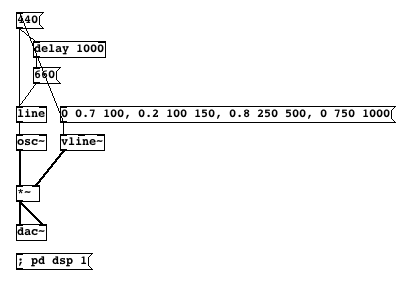
\includegraphics[scale=.5]{exemplopd1}
  \caption{2 notas num oscilador simples}
  \label{fig:exemplopd1}
\end{figure}

O fato do Pd ser uma linguagem gráfica possibilita uma facilidade de
descrição do processo de síntese sonora pelo fato de que o próprio
código é semelhante ao fluxograma tradicional de representação da
síntese.
% (inserir figura de fluxograma)

 A estrutura de um fluxograma
possui uma sequencialidade implícita (da saída final até os parâmetros
de cada gerador), mas não explicita como vão ser manipulados os
parâmetros nem qual será a duração da música.

Os ambientes Max/Msp e Pd são construídos sob o paradigma do envio
da mensagem o que não necessariamente possibilita que a linguagem seja
adequada para o armazenamento e recuperação de dados. O usuário é
praticamente forçado a colocar os dados dentro de objetos armazenadores e 
arquivos externos - bases
de dados, essencialmente - e a usar um leque de objetos como
acessórios para estocar e recuperar dados dentro do controle de
passagem de mensagens em tempo real.

A abordagem do Max/Msp quanto aos dados é ao mesmo tempo simples e
evasiva: objetos especiais de armazenagem de dados como
\textit{table}, \textit{qlist}, dentre outros são disponibilizados. Os
dados são essencialmente colocados dentro de diferentes objetos armazenadores, e
para cada tipo de armazenador uma abordagem particular é colocada
para sua estocagem, edição, interface e comunicação com o resto do
patch.

A recuperação de dados é a pior qualidade do Max porque mensagens não tem valores de
retorno. Por exemplo, uma caixa de número manipulada com o mouse não
retorna os dados da manipulação, que devem ser recuperados com outros
objetos). Os dados recuperados devem ser mandados como uma mensagem
separada de retorno. Isso leva muitos programadores de Max a achar
soluções diferentes que facilite a interação do patch com o nível
composicional.

A idéia original por trás da criação do Pd foi remover a barreira
entre a computação dirigida por eventos em tempo-real (como no estilo
do Max de passagem de mensagens) e dos dados (como em pontos num
gráfico ou notas numa partitura). Em Pd os dois (caixas de objetos e
estruturas de dados) podem facilmente coexistir em uma mesma janela.
Essa ``promiscuidade'', no entanto, não acaba deixando os objetos
funcionais e os dados intimamente conectados. De fato, no design
presente, o acesso aos dados tem que ser feito através de uma
sequência de objetos como acessórios .

Em relação a essa divisão do aspecto ``performático'' e
``composicional'' do Pd, Miller Puckette explica que

\begin{quote}
Em sua forma mais sucinta, o problema é que, enquanto temos bons
paradigmas para descrever processos (tal como em Max ou Pd, da forma como
eles existem hoje), e enquanto muito trabalho tem sido feito na parte 
de representação de dados musicais (incluindo buscas em bases de dados
de sons, passando pelos programas Patchwork e OpenMusic, e incluindo
o não finalizado editor de estruturas de dados do Pd), não possuímos
um mecanismo fluído para navegar entre esses dois mundos. \cite{puckette04:divide}
  \footnote{``in its most succinct form, the problem is that, while we have good
  paradigms for describing processes (such as in the Max or Pd
  programs as they stand today), and while much work has been done on
  representations of musical data (ranging from searchable databases
  of sound to Patchwork and OpenMusic, and including Pd's unfinished
  data editor), we lack a fluid mechanism for the two worlds to
  interoperate.'' (Minha tradução livre)} 
\end{quote}

Apesar das muitas diferenças entre
as interfaces dos ambientes de programação, 
o compositor deve manter claro o foco no resultado sonoro  da interação entre
gesto instrumental e controle de máquina.
Abordando o assunto
a partir de uma visão didático-metodológica, um projeto
composicional em Pd deve compreender a clara distinção entre os
aspectos performáticos e composicionais do ambiente. 

O que chamamos de aspectos performáticos em música interativa 
é a própria relação que criamos entre a  análise do estímulo
do instrumentista e os parâmetros de algoritmos generativos.

Sobre os aspectos composicionais me refiro a imagem global
do fazer composicional e sua relação com as ferramentas em questão.
Quando falamos de interação entre humanos pensamos em modelos
de cooperação. Mas quando pensamos em interação homem-máquina, 
pensamos em controle. Podemos pensar no conceito de influência como 
intermediário entre cooperação e controle, e mais adequado como
modelo de desenvolvimento para música interativa.

Nessa pesquisa, foram exploradas maneiras de
implementar algoritmos generativos influenciados por dados
extraídos da própria análise musical da
performance do músico.


\section{Análise}
\label{sec-analise-geral}

%% pq analise

O processo de análise musical consiste em separar elementos
do discurso com o objetivo de revelar uma possível estrutura fundamental
ou vetores de força que moldaram aspectos do resultado final.

Sobre a análise feita por computadores, Rowe acrescenta:

\begin{quote}
Há um certo paradoxo no coração da 
transferência de musical
conhecimento para uma máquina. Temos que trabalhar intensamente para fazer um programa de computador
efetuar as análises necessárias de um calouro estudante de música.
Uma vez que o trabalho é feito, no entanto, o programa pode fazer uma análise mais confiável
e certamente muito mais rapidamente do que o calouro. O computador pode entregar
descrições completas de cada acorde em um ditado em milisegundos
do seu desempenho, por exemplo. \cite{rowe2004machine}
\footnote{There is a certain paradox at the heart of the transfer of musical
knowledge to a machine. We must labor mightily to make a computer
program perform the analysis required of a freshman music student.
Once the work is done, however, the program can make analyses more reliably
and certainly much more quickly than the freshman. The computer can deliver 
complete descriptions of each chord in a dictation within miliseconds
of its performance, for example.}
\end{quote}

%% diferença entre análise e composição

Nesse sentido, a análise assistida por computador auxilia
o processo composicional durante tarefas de descrição que seriam
extremamente trabalhosas durante o processo de composição.
A diferença entre análise e composição é de que na análise, ao final do
processo, não conseguimos retornar ao pensamento composicional
original. Pelo fato de que o compositor durante seu trabalho tem a 
liberdade de criar e subverter regras, e determinar qualquer tipo de relação
entre os materiais e os procedimentos. Tornando praticamente impossível
de se modelar a atividade cognitiva durante o ato de compôr.

\begin{figure}
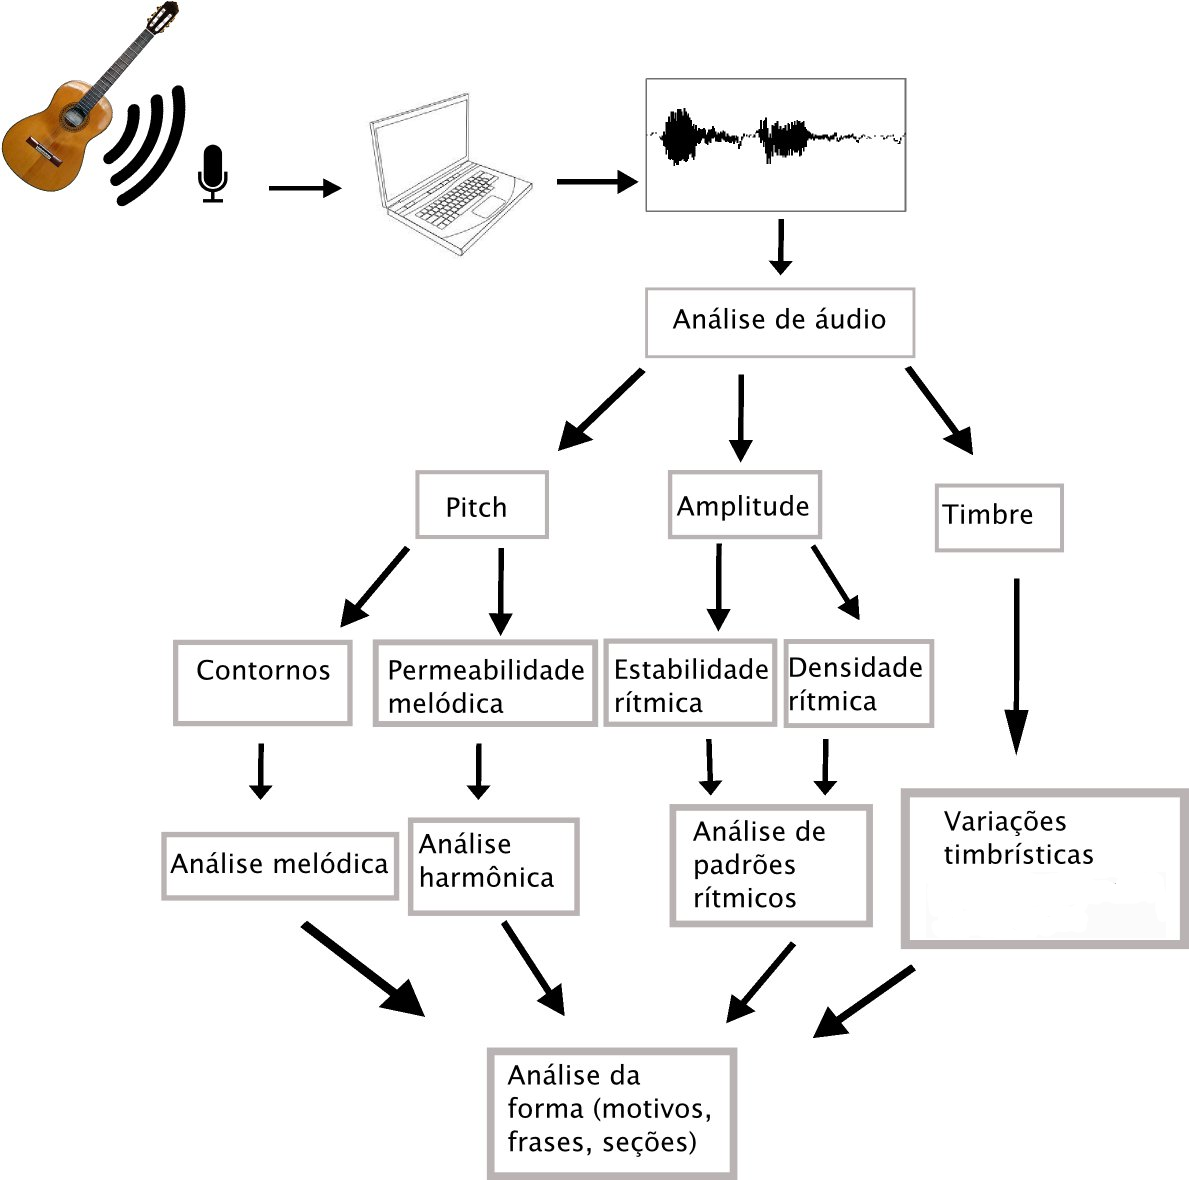
\includegraphics[scale=.9]{analise}
\caption{Diagrama ideal das etapas de análise para música interativa com instrumento tradicional}
\label{analise-geral}
\end{figure} 

Uma boa descrição dos níveis de análise que estão envolvidos em um projeto
de música interativa é fornecido por Rowe:

\begin{quote}
A primeira onda de sistemas interativos de música baseado quase exclusivamente no padrão \textit{Musical
Instrument Digital Interface} (MIDI), uma representação simbólica da música modelado
sobre o comportamento de um teclado de piano, bem como os conceitos tradicionais de notação de música.
A segunda onda toma como entrada sinais de áudio, uma sub-representação simbólica de dados que está longe
de ser mais flexível, enquanto for bem menos estruturada. \cite{rowe09:levels}
\footnote{The first wave of interactive music systems relied almost exclusively on the Musical 
Instrument Digital Interface (MIDI) standard, a symbolic representation of music modeled 
closely on the behavior of a piano keyboard, as well as traditional concepts of music notation. 
The second wave takes as its input raw audio signals, a sub-symbolic data representation that is far 
more flexible while being far less structured.}
\end{quote}


\begin{figure}
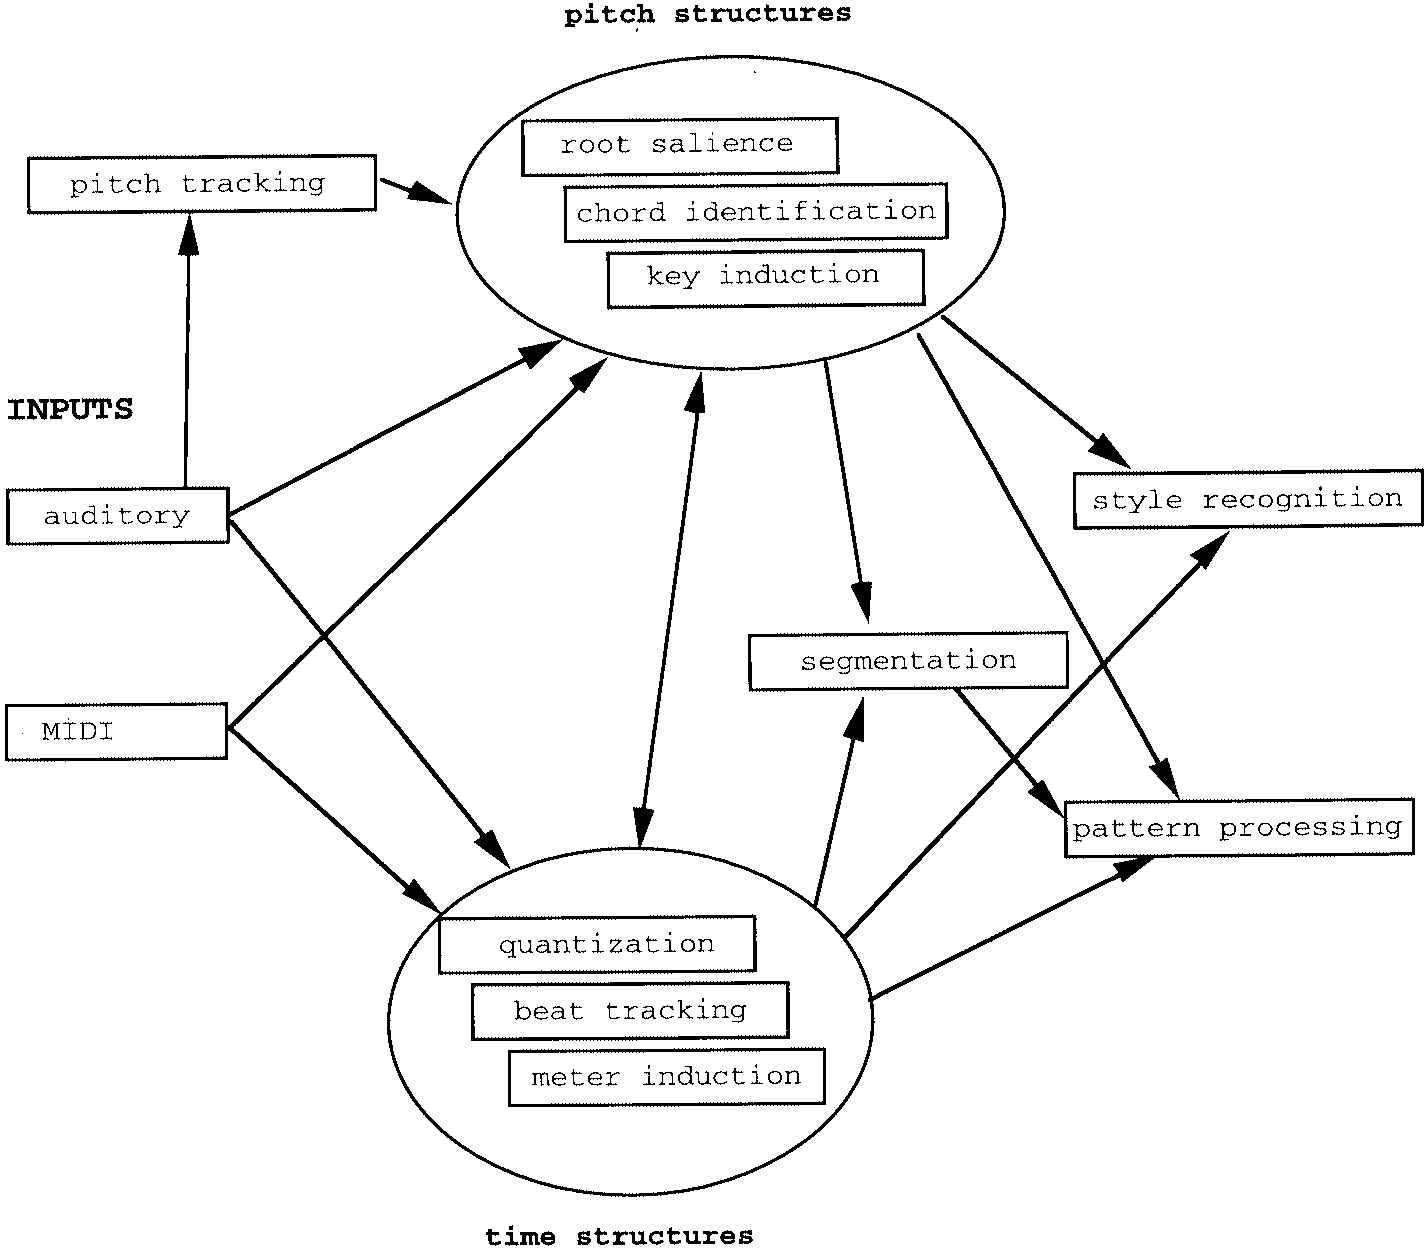
\includegraphics[scale=.25]{rowe}
\caption{Esquema de etapas de implementação de um sistema de música interativa por Robert Rowe}
\label{rowe}
\end{figure} 


Podemos ver na figura \ref{rowe} um plano geral dos níveis de análise necessários para a desenvolvimento
de uma possível ``escuta'' genérica de máquina. O sentido das flechas representa o fluxo de 
informação entre os estágios.

%% o que são os níveis simbólicos e sub-simbólicos de análise 

Podemos dividir a análise musical em níveis simbólico e sub-simbólico.
A análise musical simbólica engloba a dimensão dos símbolos musicais
estabelecidos pela notação musical como por exemplo nota, acorde, tonalidade ou compasso.
A análise musical no nível sub-simbólico diz respeito a dados que contenham informações sobre a 
descrição física do som. Leman apresenta uma descrição dos níveis simbólico e sub-simbólico 
na tentativa de estabelecer uma modelagem
computacional de esquemas cognitivos \cite{leman89}.

Enfatiza que o processamento de informação sub-simbólica abstrata pode fornecer novas formas de lidar com os aspectos
do comportamento comunicativo que até agora têm sido muito difíceis de tratar em modelos simbólicos.
Também argumenta que diferentes tipos de mecanismos de processamento de informações sub-simbólicas podem ser exploradas
e aplicadas a este campo como alternativas e/ou abordagens complementares aos modelos simbólicos.
Em particular, considera a possibilidade de representar conceitos musicais como padrões de
informações fornecidas pelo transdutor de mecanismos sensoriais, ao invés de símbolos abstratos onde o conteúdo
é separado da forma. Por fim argumenta em favor de uma representação analógica musical
com base na Psicoacústica e propõe este sistema como uma alternativa para a abordagem de discurso lógico da representação musical \cite{leman89}.

% \begin{quote}
% O processamento de informação sub-simbólica abstrata pode fornecer novas formas de lidar com os aspectos
% do comportamento comunicativo que até agora têm sido muito difíceis de tratar em modelos simbólicos.
% Parte de nossa análise é mostrar que as atividades musicais, como ouvir e compor partem em
% grande escala de princípios dinâmicos do que é comumente chamado de percepção e/ou imaginação auditiva.
% Argumenta-se que diferentes tipos de mecanismos de processamento de informações sub-simbólicas podem ser exploradas
% e aplicadas a este campo como alternativas e/ou abordagens complementares aos modelos simbólicos.
% Em particular, considerar a possibilidade de representar conceitos musicais como padrões de
% informações fornecidas pelo transdutor de mecanismos sensoriais, ao invés de símbolos abstratos onde o conteúdo
% é separado da forma. Isto envolve uma mudança de representações musicais proposicionais para representações analógicas
%  (onde o conteúdo está contido na forma). Representações analógicas de música
% não foram totalmente exploradas até agora. Argumentamos em favor de uma representação analógica musical
% com base na Psicoacústica e propor este sistema como uma alternativa para a abordagem de discurso lógico da representação musical.
% Um exemplo é dado de um sistema de auto-organização com uma estrutura global emergente
% com base neste tipo de representação. \cite{leman89}
% 
% \footnote{Abstract Subsymbolic information processing may provide new ways of dealing with aspects of 
% communicative behavior that have hitherto been very hard to deal with in symbolic models. 
% Part of our analysis is to show that musical activities such as listening and composing draw at 
% large on dynamic principles of what is commonly called perception and/or auditory imagination. 
% We argue that different types of subsymbolic information processing mechanisms might be explored 
% and applied to this field as alternatives and/or complementary approaches to symbolic models. 
% In particular, we consider the possibility of representing musical concepts as patterns of 
% information provided by sensory transducer-mechanisms, rather than abstract symbols where content 
% is divorced from form. This involves a shift from propositional representations of music to analogical 
% representations (where content is contained in the form). Analogical representations of music 
% have not been fully explored until now. We argue in favor of an analog musical representation 
% format based on Psychoacoustics and propose this system as an alternative to the speech-logics 
% approach to music representation. An example is given of a self-organizing system with an emerging 
% global structure based on this type of representation.}
% \end{quote}



Apesar da análise ser um dos principais elementos dessa pesquisa, é preciso
definir que o objeto final é uma ferramenta de composição e não de análise.
Nesse caso, a análise serve como uma etapa da composição. A composição em si
se dá no próprio momento da performance. Cada execução musical realizada
com SInCoPA terá elementos diferentes, mesmo que o instrumentista execute
o mesmo trecho musical, as escolhas sonoras do programa terão variações.
Isso se deve pelos fatos de que pequenas variações de tempo e dinâmica 
vão interferir no resultado da análise e portanto irão afetar os parâmetros
dos algoritmos geradores.

Normalmente pensamos na análise
como uma ação posterior ao processo de composição. Nessa pesquisa a etapa
de análise é um dos pontos indispensáveis do processo de composição.
Um possível diagrama ideal das etapas de análise, necessárias a
constituição de um sistema de interação musical com um instrumento
tradicional pode ser visto na figura \ref{analise-geral}. Onde temos um
primeiro nível sub-simbólico de análise do áudio e primeira segmentação
e classificação de notas (pitch), amplitude, ataque e tempo entre ataques (IOI\footnote{Inter-
Onset-Interval \cite{rowe2004machine}}) e timbre.

O nível simbólico aparece abaixo em duas linhas compreendendo primeiro análise de 
contornos, permeabilidade melódica, estabilidade rítmica e densidade rítmica. 
Que se subdividem em análise melódica, harmônica, de padrões rítmicos e de 
variações timbrísticas. Uma hipótese é que no final dessa sequência de análises,
os resultados propiciarão elementos para um mecanismo mais completo de análise da
forma.



No recorte dessa pesquisa, foram definidas e apontadas ferramentas que compreendem o nível
sub-simbólico e a primeira classe do nível simbólico. 

%% desenvolver mais

Uma outra análise pode ser feita sobre o resultado final da interação, quando se obtém
o conjunto de dados e estruturas geradas pelo músico e pelo sistema. Idealmente, na análise desses 
dados não há como separar
a influência do sistema na execução do músico. O resultado da análise desses dados pode revelar
estruturas arquetípicas passíveis de classificação, o que poderia ser chamado de taxonomia 
da interação. Tal qual a espectromorfologia \cite{smalley:86} é uma taxonomia geral
para análise de música eletroacústica\footnote{Nesse sentido podemos apontar os artigos
``Por uma morfologia da interação'' \cite{menezes2006musica} e ``Morphological notation for interactive electroacoustic music'' 
\cite{Patton:2007} como seminais na definição dessa taxonomia.}.





\subsection{Análise de áudio}
\label{sec-audioanalise}


O objetivo da análise de áudio é extrair informações em tempo-real
que possam ser convertidas em elementos de simbologia musical, como notas, durações e dinâmica.
A partir dessa conversão podemos implementar outras análises no 
âmbito dos elementos musicais, como análise de contornos, estabilidade e 
densidade rítmica e outros modelos de análise aplicados aos elementos
simbólico-musicais. 

Outro nível de informação é fornecido pela análise do timbre, capaz
de revelar detalhes do comportamento espectral de cada evento, que no caso de uma 
performance instrumental, pode ajudar a expôr aspectos narrativos.

Existe uma certa dificuldade na tentativa de definir uma ferramenta genérica de análise de áudio 
que funcione igual em diferentes plataformas e configurações .
Isso se dá por conta das muitas variáveis envolvidas, como diferentes instrumentos, microfones, 
captadores, placas de som e outros fatores.
A dificuldade varia de acordo com as configurações possíveis. A captura e análise de áudio
 de instrumentos monofônicos e que usam captadores é bem mais estável
do que situações que envolvem microfones e instrumentos polifônicos.

\begin{figure}
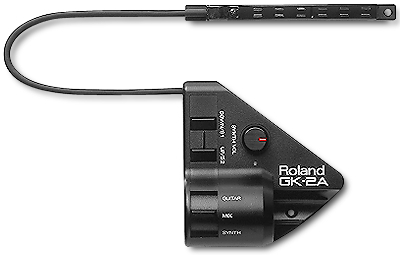
\includegraphics[scale=.5]{gk-2a}
\caption{Captador hexafônico GK-2A da Roland}
\label{gk-2a}
\end{figure} 


A experiência de música interativa usando violão ou guitarra elétrica passa necessariamente
pela problemática do reconhecimento de frequências nos trechos de sinal polifônico.
Uma solução seria o uso de um captador hexafônico para captar o áudio separado de
cada corda. Uma das principais opções comerciais é o captador GK-2A da Roland.
Ele funciona em conjunto com um módulo de hardware vendido separado que faz o trabalho de conversão 
de áudio para MIDI, incluindo ainda algumas funcionalidades, como arpegiador automático
e mudança de canal controlados por pedal  e banco de timbres.
Outras soluções incluem o desenvolvimento experimental de hardware tanto na implementação
do próprio captador hexafônico, quanto na construção de um módulo amplificador de seis
canais separados.

 
Miller Puckette, descreve sua própria experiência na construção de um sistema interativo
para guitarra preparada com captador hexafônico:

\begin{quote}
Eu estive trabalhando em um projeto de longo prazo para projetar um
instrumento de música computacional para tentar trazer à tona e enfrentar algumas das dificuldades encontradas pelos
músicos que tentam usar computadores em performance ao vivo. O instrumento é baseado numa guitarra elétrica compacta
(Steinberger/Gibson), com um captador adicional de seis cordas separadas (Roland). Não encontrando um
amplificador barato e compacto de 6 canais no mercado, eu projetei e construí um muito simples.
Este é conectado a um computador usando uma interface multicanal PCI (Midiman). Um patch de Pd, rodando em
linux, em seguida, executa uma série de transformações interessantes sobre os seis sinais de áudio, e mistura-os
para saída em estéreo.

Isto é completamente diferente do padrão `` sintetizador de guitarra ", que mapeia as cordas para conduzir
sintetizadores. Tais instrumentos cometem muitos erros audíveis, e eles também sofrem com a latência adicionada do mapeamento. 
No instrumento aqui descrito, a latência de todo o processo é
somente a do Pd propriamente, cerca de 10 milissegundos (provavelmente não é difícil reduzi-la a 5 ou 6 usando
correções em tempo real do kernel, mas eu preferi usar uma distribuição pronta de linux) \cite{Puckette_patchfor}.
\footnote{I've been at work on a long-term project to design a rather personalized 
computer music instrument to try to bring out and confront some of the difficulties encountered by 
musicians trying to use computers in live performance. The instrument is based on a compact electric 
guitar (Steinberger/Gibson) with an added six-string separated pickup (Roland). Not finding an 
inexpensive and compact 6-channel preamp on the market, I designed and built a very crude one. 
This is interfaced to a computer using a multichannel PCI interface (Midiman). A Pd patch, running in 
linux, then performs a variety of interesting transformations on the six audio signals, and mixes them 
to stereo for output.

This is entirely different from standard ``guitar synthesizers" which pitch track the strings to drive 
synthesizers. Such instruments make lots of audible mistakes, and they also suffer from the added latency 
the comes from the pitch tracker. In the instrument described here, the latency of the whole affair is 
only that of Pd itself, about 10 milliseconds (it's probably not hard to reduce it to 5 or 6 using 
real-time kernel patches but I preferred to use off-the-shelf linux).}
\end{quote}

Da mesma maneira como é mostrado nessa pesquisa a análise de áudio operada em um sinal de áudio
monofônico, poderíamos implementar um módulo de análise para cada uma das seis cordas de uma guitarra.
O Pd é um ambiente de programação com bons recursos de análise de frequência e amplitude. Vários
objetos são disponibilizados como filtros, conversores e algoritmos de estimativa de frequência fundamental.
Podemos afirmar que a análise de áudio monofônico com objetos padrão do Pd tem uma boa estabilidade e
precisão. Dentro do escopo dessa pesquisa são aprofundados experimentos em análise de áudio monofônico,
ainda que muitas vezes os testes tenham sido feitos com instrumentos polifônicos como violão e 
guitarra, executando linhas melódicas.


 
\subsection{Representação musical}

A análise do áudio de entrada em tempo-real é convertida em uma representação simbólica de 
elementos musicais. A primeira segmentação da análise
de áudio, diz respeito ao nível da nota, sua frequência (pitch),
amplitude e ataque. O resultado da análise de áudio é convertido
em um fluxo de eventos MIDI.

Nessa pesquisa, optou-se pelo protocolo MIDI como um intermediário
entre as descrições da análise de áudio e o conjunto de representações
simbólicas envolvidas no sistema. Os algoritmos de geração
de material musical usam formatos variados de representação musical 
além do MIDI, de acordo com a necessidade de cada caso.

Muitos autores já discorreram sobre os limites da representação musical
com o protocolo MIDI. O objetivo é usar o MIDI como protocolo de comunicação
com outros programas para manipulação dos algoritmos geradores.
De certa maneira a forte relação do protocolo MIDI com a música instrumental
é um ponto positivo nessa pesquisa que prevê interação musical através de 
instrumentos tradicionais. 
%%original: http://www.lamut.musica.ufrj.br/lamutpgs/rcpesqs/02coper.htm
A reação dos compositores de música eletroacústica em relação ao protocolo MIDI
é bem exposto por Rodolfo Caesar :

\begin{quote}
A música eletroacústica e o protocolo MIDI não foram feitos um para o outro: a especificidade da 
primeira não encontra ressonância imediata no segundo. Se quisermos fazer uso do protocolo MIDI 
para a música eletroacústica, é preciso algum empenho contra suas limitações. \cite{caesarcopa} 
\end{quote}


Podemos entender esse tipo de reação, se pensarmos que o MIDI foi um padrão
que percorreu desde os estúdios de música comercial até as pesquisas experimentais
de música interativa nos anos 80. Robert Rowe explica:

\begin{quote}
As primeiras implementações de sistemas de som interativos eram feitas geralmente com \textit{Musical
Instrument Digital Interface} (MIDI) padrão. O padrão MIDI tem sido reconhecido desde o seu início
por ser lento e limitado no seu âmbito de representação. A dependência de equipamento MIDI externo tem
condenado uma geração de trabalhos interativos para a obsolescência, assim que o hardware necessário se torna indisponível.
Máquinas mais rápidas e mais baratas tornaram possível nos últimos anos a realização de análise, síntese, amostragem, 
e os efeitos sobre a CPU de um computador de uso geral pessoal, em simultâneo com a
execução do software em nível de controle. \cite{rowe05}
\footnote{
 Interactive music systems in early implementations usually made use of the Musical
Instrument Digital Interface (MIDI) standard. The MIDI standard has been recognized since its inception
to be slow and limited in its scope of representation. Reliance on outboard MIDI gear has
doomed a generation of interactive works to obsolescence as the requisite hardware becomes unavailable.
Faster and cheaper machines have in recent years made it possible to perform analysis, synthesis,
sampling, and effects on the CPU of a general purpose personal computer, simultaneously with the
execution of control level software.}
\end{quote}


MIDI é usado na prototipação de algoritmos que dizem respeito as questões de 
altura, duração e dinâmica. De maneira geral, não faz sentido usar MIDI em situações 
musicais que não são pensadas sob o paradigma da nota tocada. O que não é
necessariamente uma regra, pois ainda nesses casos o protocolo MIDI pode ser
útil.

No nível da representação simbólica, os dados são convertidos para MIDI e manipulados
com estruturas híbridas como arrays e listas de números. Apesar de obsoleto, muito desenvolvimento
ainda é feito pensando no protocolo MIDI. O protocolo OSC\footnote{Open Sound Control} permite que
sejam enviados pacotes de dados via rede pelo protocolo UDP/IP. Nesses pacotes podemos incluir
mensagens MIDI inteira ou fragmentadas e reconstruídas na extremidade de quem está recebendo.
O modelo de representação musical no Pd é uma combinação dos principais protocolos disponíveis para
música interativa. Isso permite uma definição híbrida na representação dos dados, como é o caso
nessa pesquisa.


\subsection{Segmentação e Classificação}


Segmentação é o processo pelo qual, eventos musicais são organizados
em grupos. Existem diversas razões que reforçam a importância da 
segmentação: primeiro, porque nós, seres humanos, percebemos música
por trechos em vários níveis e um sistema interativo que procura emular
o comportamento de um músico deve estar apto a formar grupos durante
a análise, similar ao que o músico humano percebe durante a escuta.

A implementação de um segmentador que simule o ato de escuta de um ser 
humano é um trabalho específico que foge do escopo dessa pesquisa. Entretanto,
podemos através da literatura da área e experimentação criar pequenos
mecanismos que incrementam a capacidade de segmentação do sistema.

O primeiro elemento a ser pensado na segmentação de um fluxo musical,
são os silêncios. Na concepção de diálogo entre ser humano e máquina,
é imprescindível que a máquina esteja preparada para reconhecer automaticamente
as pausas no discurso. Cada pausa deve ser cateorizada como respiração, fim de frase,
fim se seção ou fim da peça.

Vamos ver que na implementação podemos definir um sistema híbrido de segmentação
entre processos automáticos com processos de segmentação ``manual'' pelo músico.
Quanto mais automático o processo de segmentação, mais refinado se torna
o sistema de análise e classificação. 

A classificação de durações passa por dois filtros. O primeiro
é o classificador de estabilidade rítmica, que através da média das durações 
entre ataques de notas de um recorte de segmento calcula e classifica
o segmento entre estável ou instável.
Outro filtro classificador é o de densidade rítmica, que por sua vez classifica
o segmento em questão entre alta e baixa densidade, podendo ainda estabelecer
matizes entre os dois extremos. . 

A classificação de alturas classifica contornos e probabilidade de recorrência
de cada nota. A análise da direcionalidade e atratividade melódica pode ser abstraída
em modelos de análise algorítmica \cite{lerdahl2001}, e atualmente vem sendo modelada para 
implementação em sistemas interativos \cite{rickgrahan}.
A análise e classificação do timbre é extensamente apresentada e implementada em dois
trabalhos em \cite{brentcepstral} e \cite{monteiro}.

No caso dos geradores de processamento de áudio, a segmentação é feita 
através de um teclado alfanumérico modificado usado como pedal. A função
do pedal é criar pontos no tempo que representam o começo de determinados
processos. Por exemplo o começo de leitura de um ponto de loop, ou o começo
e fim de gravação de um segmento para ter o áudio processado.

Essa funcionalidade poderia ser expandida criando-se botões de controle
e sensores, posicionados no próprio corpo do instrumento. Chegando próximo ao conceito
de ``instrumento aumentado'' ou ``\textit{hyperinstrument}'' \cite{hyperinstrumento}. 
Apesar de fugir do recorte dessa pesquisa, essa possibilidade
de expandir fisicamente o instrumento é um recurso muito útil em sistemas de
música interativa. Isso pode facilmente ser feito com a plataforma Arduino\footnote{Arduino
é uma plataforma de prototipação eletrônica para aplicações interativas. Disponível em: 
www.arduino.cc}, integrada dentro do Pd. 




\subsection{Interação e Automação}

Interação e Automação de certa maneira refletem ânimos tanto do
fazer composicional de música instrumental, onde o compositor
escreve em notação tradicional (automação) enquanto o instrumentista
interpreta (interação). Ou então ao contrário como em alguns procedimentos
de composição eletroacústica, onde o compositor interage com os materiais
e as ferramentas no estúdio para gravar uma imagem sonora automatizada.

O diálogo musical é desenvolvido com o estímulo
do instrumentista e a resposta do computador. Os dados
da análise dessa execução, alimentam um leque de algoritmos
interativos que tem seus parâmetros alterados pela análise.

Nesse sentido podemos classificar os algoritmos composicionais
em sequenciados, generativos e transformativos \cite{rowe93:interactive}.
Ao longo da descrição de SInCoPA iremos descrever algumas implementações
dessas três categorias.

Uma característica de um sistema interativo é a capacidade de criar
automações em tempo-real. Nesse sentido podemos pensar em um sequenciador
que seja controlado em tempo real pela performance do músico.

Diferentes graus de interação e automação são explorados ao longo do
trabalho que prevê algoritmos generativos, baseados nos dados da análise. 
Além de algoritmos transformativos tanto do material musical simbólico,
abstraído da análise, quanto do próprio áudio, como processamento de áudio
através de fragmentação, repetição e processamento de amostras de áudio.


\section{Poética da interação}


A própria imersão nas técnicas de composição assistida por computador de certa
maneira conduz uma estetização na concepção musical. Essa estetização visível
pode ser considerada positiva, pois não existe a pretensão de com um sistema 
de interação homem-máquina simularmos precisamente a interação musical entre
humanos. A intenção é aprofundar as relações de interação musical homem-máquina
para a possível emergência de novas idéias expressivo-musicais. 

A ferramenta enquanto objeto técnico povoa a imaginação do compositor. A possibilidade
da gravação e repetição do próprio áudio emitido automaticamente cria uma paleta de
possibilidades inventivas. Enquanto procedimento, a repetição sempre fez parte da linguagem
musical. O desejo pela repetição pode ser um arquétipo presente em nossa cultura
muito antes do surgimento das tecnologias de gravação de áudio. Uma espécie
de variação da busca de obra de ``arte total'' idealizado por Richard Wagner: 


\begin{quote}
 Nos loops de áudio quanto mais semelhança entre as partes final e inicial, mais mascarada fica a
emenda. Quanto mais disfarçada a parte da ‘cola’, mais garantido o efeito de um ‘sem fim’. A finalidade
desta emenda bem-feita manifesta premonitoriamente (no século XIX), o desejo de ‘imersão’ de algumas
artes ‘digitais’, ‘multimídias’ ou ‘tecnológicas’, projeto típico de décadas finais do século XX e início do
XXI. O sonho da ‘obra de imersão total’ – que portanto depende de um confinamento e um mascaramento -
é criteriosamente representado no filme ‘Brainstorm’ (1983), de Douglas Trumbull, no qual um grupo de
cientistas inventa um gravador que registra integralmente as emoções humanas. O grau máximo e total de
satisfação onanista é perseguido por um dos cientistas - personagem representando o mau uso da ciência -
que finalmente realiza seu super-loop:
Clip: trecho de ‘Brainstorm’, em que se vê o ‘mau’ cientista aprisionado ao loop de seu orgasmo, gravado na
companhia de uma prostituta, que não receberá royalties pelo uso de sua imagem. \cite{caesarloop}
\end{quote} 

Alguns aspectos filosóficos sobre a questão da repetição na composição contemporânea,
são extensamente desenvolvidos por Sílvio Ferraz no seu livro 
``Música e repetição: a diferença na composição contemporânea'':
 
\begin{quote}
O eterno retorno não pode significar o retorno do Idêntico, pois ele supõe, 
ao contrário, um mundo (o da vontade de potência)em que todas as identidades 
prévias são abolidas edissolvidas. Retornar é o ser, mas somente o ser do devir. 
O eterno retorno não faz “o mesmo” retornar, mas o retornar constitui o único 
Mesmo do que devém. Retornar é o devir-idêntico do próprio devir. Retornar é, 
pois, a única identidade,mas a identidade como potência segunda, a identidade da 
diferença, o idêntico que se diz do diferente, que gira em tornodo diferente. 
Tal identidade, produzida pela diferença, é determinada como “repetição”. \cite{ferraz1998musica}
\end{quote}


Quando pensamos em estímulos composicionais, nos deparamos com expressões
vagas de descrição de emoções e fragmentos de memória. Essas descrições
ajudam o compositor a definir caminhos para criação de narrativas e 
objetos sonoros. O poder expressivo da música interativa é a capacidade
de fusão e contraste em diversos níveis. Desde o nível cultural que prevê
uma bagagem de idiomas e gestos próprios, tanto do domínio intrumental quanto
do campo da computação musical, até o nível sub-simbólico, com as possilidades
de fusão espectral do som:

\begin{quote}

Para haver fusão entre as escrituras instrumental e eletroacústicas,
será necessário que haja \textit{transferências localizadas} de 
características espectrais de uma esfera de atuação à outra.
Aquilo que se funde com outra coisa, assim o faz pela \textit{similaridade
absoluta}, com esta outra coisa, de ao menos um aspecto de sua 
constituição. Nesse sentido, tratando-se de sons eletroacústicos 
pré-elaborados em estúdio, a eleição do material constitutivo de partida
adquire grande relevância: será mais plausível trabalhar, sobre suporte,
com sons oriundos dos próprios instrumentos do que com proveniências
díspares, sem qualquer relação de origem com a materialidade corpórea
dos instrumentos utilizados. Ainda que as transformações em curso possam ser
bem drásticas, o uso de material constitutivo similar faz com que
haja preponderância em conservar algum aspecto energético que confira
identidade às texturas sonoras resultantes. \cite{menezes2006musica}
\end{quote}


Na música interativa pode-se argumentar que a fusão se dá também no nível
físico do gesto. Quando a interação é mais reativa e auditivamente reconhecível
como diálogo interativo, a própria percepção do todo se aproxima de uma
fusão sonora. Quando se define métodos de interação musical devemos levar
em conta experimentos que explorem as fronteiras do que o músico entenda
que seja uma escala de fusão sonora e gestual. Aí se coloca uma questão
importante que é o papel do músico intérprete. A formação tradicional
do intérprete musical nem sempre contempla as nuances e dúvidas presentes na construção
de uma interpretação de música interativa. 

\begin{quote}
Como quer que seja, na fusão instaura-se uma condição de \textit{dúvida}.
Em certa medida, fusão implica propositadamente, da parte do compositor,
\textit{confusão} para o ouvinte,
....
o ouvinte recai em constantes dúvidas
acerca da natureza daquilo que se ouve: se advém do instrumento ou da 
emissão eletroacústica, se se opera ao vivo uma dinamização espacial, harmônica
, tímbrica e temporal da escritura instrumental ou se será defronte de
estruturas pré-elaboradas em estúdio, constituidas a partir dos próprios
instrumentos ou a estes timbricamente correlatas. Em relação a proveniência
sonora, quanto mais ``confuso'' estiver o ouvinte em face daquilo que
o ouve, tanto mais ele sentirá como efetivamente integradas as partes
constitutivas da obra mista; os "dois planos" pressupostamente independentes
e unidos apenas por contingência,
... 
Ainda que de forma alguma hegemônico, o \textit{estado de
dúvida} traduz-se como momento supremo da interação. \cite{menezes2006musica}
\end{quote}

Certamente a dúvida é uma das características mais importantes na composição
de música interativa. Nesse sentido, um aspecto fecundo é a dúvida do músico
intérprete. O fato do instrumentista não conseguir entender/controlar a resposta
da máquina pode levar a composição a um patamar de constante descoberta e inovação.
Acredito que essa seja uma importante atitude composicional em um projeto de 
música interativa, pois leva o instrumentista a atitudes mais radicais na 
busca por variação e contraste musical.

\begin{quote}
O contraste, por sua vez, ancora-se sobretudo na diferença e na 
\textit{distinção absoluta}. Em seus momentos mais acentuados, faz com
que a emissão instrumental ou a eletroacústica assumam o papel estrutural
do silêncio ou, ao contrário, adquiram autonomia temporal e até mesmo
excludente com relação à outra esfera sonora. \cite{menezes2006musica}
\end{quote}

Fusão e contraste são aspectos que sempre estiveram ligados a prática
composicional. Na composição de música interativa encontramos um ponto onde
vários eixos se cruzam e diversos matizes de fusão e contraste podem
conduzir uma poética musical interativa.
O embate sonoro entre homem e máquina pode por fim revelar os aspectos
essencialmente humanos que se possa expressar musicalmente. 


\subsection{Papel do músico na interação homem-máquina}


Do ponto de vista do instrumentista, alguns aspectos podem ser apontados nessa pesquisa.
Por um lado o gesto instrumental é ao mesmo tempo o impulso inicial e uma espécie
de ``cola'' narrativa. Por mais que se forneçam elementos de análise para o sistema
computacional, as narrativas geradas tendem a ser repetitivas e óbvias. Nesse contexto
se abre um campo grande para experimentação instrumental. Se pensarmos na lei da ``boa continuidade''
na \textit{Gestalt}, podemos investigar que o instrumentista treinado tende a completar
os espaços de pausa e realizar movimentos cadenciais. Criando significado narrativo
para gestos a princípio ligados pelo vínculo com a análise do instrumentista, mas muitas
vezes sem conexão interna.

Outro campo de possível investigação é a análise de em que
nível a prática instrumental com um ambiente reativo como
esse proposto aqui, influencia o gestual do instrumentista.
Um estudo minucioso poderia incluir a avaliação do gestual
instrumental antes e depois do contato do instrumentista com 
o sistema.

De certa maneira, o instrumentista treinado é o profissional
mais preparado para conceber um sistema interativo dessa natureza.
Primeiro porque conhece os detalhes de comportamento sonoro de seu
instrumento a partir da prática instrumental ao invés da pura análise
espectral. Em segundo lugar porque entende o idioma instrumental
de maneira empírica. A complicada trama entre fisicalidade instrumental
e narrativa sonora exige um conhecimento empírico sobre a prática
instrumental.


%% aqui escrever uns 2 parágrafos concluindo o 1º capitulo

Nesse capítulo foi exposta a linha geral de pesquisa que conduziu
o desenvolvimento desse trabalho.
Num primeiro momento, a problemática da pesquisa se voltou ao ato composicional
através da computação e na relação das diferentes interfaces computacionais
com o pensamento criativo musical. Se faz necessária uma reflexão sobre
as diferentes ferramentas e linguagens computacionais levando-se em conta
a mudança de paradigma compositivo colocado pelas novas tecnologias.

Foram expostos os principais conceitos referentes a análise e sua
classificação em diferentes níveis de representação.
Dentro de um projeto de música interativa é essencial a determinação de uma
metodologia de análise que leve em conta a distância entre a representação
física do fenômeno sonoro e a definição de elementos simbólicos musicais.

Ainda foram expostos conceitos capazes de influenciar um planejamento
composicional em música interativa, como por exemplo a separação binária entre
automação e interação. Por fim, foram expostas algumas reflexões sobre a
possibilidade de uma poética presente na interação homem-máquina e sobre
o papel do compositor-instrumentista na composição de música interativa.
Os problemas conceituais aqui apresentados, apesar de não possuirem
conclusões definitivas, são melhor apreciados e compreendidos ao longo
da exposição técnica de SInCoPA.



\chapter{Trabalhos relacionados}
\label{sec:rev}

O conceito de interação entre uma performance musical e computador vem
sendo definido nas últimas 3 décadas, e possui diferentes nuances de definição
a depender do contexto de idioma e prática musical a que se refere e a tecnologia
em que é implementada. A descrição ''sistemas musicais interativos``, é um
termo introduzido no livro \textit{Interactive Music Systems} 
\cite{rowe93:interactive} e definido como ''sistemas de música 
computacional em que as mudanças de comportamento são responsivas a um
estímulo musical``. Interação em um sentido mais global pode ser definida: 
  ''Interação tem dois aspectos:
tanto as ações do performer afetam a saída do computador, ou as ações do computador
afetam os resultados do performer`` \cite{garnett:2001}.

Isso pode ser comparado a comunicação entre músicos no modelo de  música de 
câmara tradicional onde dois ou mais músicos realizam música escrita, improvisada 
ou mista \cite{winkler93:interactive}.

Em relações interativas mais complexas, ``um compositor pode
delegar vários papéis a um computador num ambiente de música interativa. Ao
computador pode se dar o papel de instrumento, performer, regente, e/ou compositor.
Esses papéis podem existir  simultaneamente e/ou mudar continuamente''\cite{lippe:2002}.



A pesquisa em sistemas musicais interativos vem nos últimos anos
deixando de ser uma abstração teórica e se transformando em realidade
concreta. O corpo de áreas de pesquisa compreende temas como cognição
musical, computação e teoria e análise musical.


Podemos apontar a multi-disciplinaridade dessa pesquisa como pertencente 
ao escopo de uma disciplina genérica emergente denominada Design de Interação(ID).
%%o que é ID
A maioria dos tratados e especificações da ID se referem a interação para a web
e interação homem-máquina focada em paradigmas comerciais. Ainda que essa pesquisa busque
uma maior interação homem-máquina num nível de funcionalidade auxiliar a poética musical, algumas idéias e 
pensamentos da ID podem ser úteis na organização do desenvolvimento do SInCoPA. 
Como por exemplo os sete estágios da ação \cite{norman06:design} onde descreve que para 
descobrir o que torna a
execução de uma tarefa difícil é necessário examinar a
estrutura de uma ação. Ele propõe sete estágios: um para
meta, três para execução e três para avaliação. A seguir cada
estágio será detalhado.
Formalizar a meta – o primeiro estágio refere-se a decisão de
realizar alguma coisa, ou seja, estabelecer a meta a ser
alcançada. A meta é algo a ser atingido, e nem sempre é bem
definida.
Formalizar a intenção – de acordo com Norman as
metas não definem precisamente o que deve ser feito. Para
se transformar em ações as metas precisam ser traduzidas
em definições específicas do que deve ser executado, o autor
denomina essas definições de intenções. As intenções são
ações específicas que foram realizadas para atingir as metas.
Portanto, após determinar a meta a ser alcançada deve-se
determinar quais serão as ações a serem executadas para
atingir a meta estabelecida.
Especificar a ação – após definir as intenções, essas devem
ser traduzidas por um grupo de comandos internos, ou seja,
uma sequência de ações que possam ser desempenhadas de
modo a satisfazer a intenção. Ressalta-se que até esta etapa
tudo ocorre mentalmente.
Executar a ação – com a sequência de ações definidas,
deve-se colocar em prática o que foi estabelecido.
Ter a percepção do estado do mundo – esta fase esta
intimamente relacionada com a posterior (interpretar o estado
do mundo). Neste momento, deve-se perceber as alterações
ocorridas no ambiente que ocorre a ação.
Interpretar o estado do mundo – após a percepção deve-se
analisar e compreender o que ocorreu no ambiente em
questão.

Avaliar o resultado – por fim, deve-se comparar o resultado
obtido com a meta estabelecida para concluir se o que foi
planejado foi de fato alcançado.
Norman deixa claro que estes estágios não são regras,
são apenas um modelo aproximado para compreender como
os indivíduos fazem as coisas. Esses estágios podem facilmente
ser pensados como um método para um design do desenvolvimento 
de um projeto interativo. Apesar da presente pesquisa não usar de 
maneira sistemática esse método, esses estágios pode servir como
método de avaliação ao final do desenvolvimento.

Outra área emergente que possui muitas características em comum com essa
pesquisa é a disciplina que se chama ''Realidade Aumentada`` (RA), que é uma linha de pesquisa dentro da ciência da computação que lida com 
integração do mundo real e elementos virtuais ou dados criados pelo computador. Atualmente, a 
maior parte das pesquisas em RA está ligada ao uso de vídeos transmitidos ao vivo, que são 
digitalmente processados e “ampliados” pela adição de gráficos criados pelo computador.

A definição de Ronald Azuma 
sobre a Realidade Aumentada \cite{azuma97:ar} é uma descrição genérica que pode nos auxiliar na delimitação teórica. 
Ela ignora um subconjunto do objetivo inicial da RA, porém é entendida como uma representação 
de todo o domínio da RA: Realidade Aumentada é um ambiente que envolve tanto realidade virtual 
como elementos do mundo real, criando um ambiente misto em tempo real.
Azuma define a Realidade Aumentada como um sistema que:
\begin{itemize}
 \item combina elementos virtuais com o ambiente real; 
  \item é interativa e tem processamento em tempo real; 
  \item  é concebida em três dimensões.
\end{itemize}

    
Se pensarmos em uma realidade aumentada sonora, chegaremos a uma definição que se afina 
com alguns objetivos dessa proposta.
Um projeto similar nesta busca de interatividade sonora é o RjDj - uma companhia que desenvolve 
software de áudio para IPhone, baseado em Pure data. Cada software 
é chamado "cena" e é feito em Pd. Cada "cena" se ocupa em explorar alguns 
aspectos sonoros do ambiente e interagir responsivamente com esses sons, criando uma 
outra narrativa com elementos reais a volta. A experiência de escutar sua voz distorcida,
somada a outros sons do ambiente sonoro, provoca uma mudança de percepção até então 
explorada somente no circuito da música eletroacústica e experiências de laboratório. 
O RjDj possibilita experiências sonoras únicas, integrando o som do ambiente , 
inventividade sonora e re-combinação através de software. Pode-se considerar o 
RjDj um real experimento em realidade aumentada no campo sonoro, uma vez que uma ''cena``
pode ''harmonizar`` eventos sonoros acontecidos ao redor, ou modificar o andamento de
uma música pelo sensor de movimento do IPhone. Os inventores do RjDj, costumam chamar 
o sistema deles de ''droga digital``, pois é capaz de alterar o estado de percepção sonora,
de acordo com a cena carregada e com os estímulos do ambiente e do usuário. 



A pesquisa em computação musical tradicionalmente se utiliza de
desenvolvimentos em redes neurais artificiais (ann – artificial neural
networks), agentes inteligentes artificiais e outros ramos da pesquisa
em inteligência artificial (IA); a produção musical oferece ótimos
casos - teste para a pesquisa em IA. Esse projeto apresenta o desafio
de construir um sistema que use elementos da pesquisa em IA
possibilitando uma interação próxima com músicos humanos e que seja
uma base de trabalho funcional para a prática artístico-musical. Isso
é mais fácil de falar do que de fazer; as habilidades de músicos
humanos em fluidez de ação, capacidade de resposta a situações novas e
referências culturais, transformam a capacidade de interação dos
sistemas computacionais numa árdua tarefa. O fato do sistema ter como
paradigma a criação de música em tempo-real ainda requere uma grande
dimensionalidade de descrições, rápido aprendizado, respostas e
efetiva capacidade de antecipação. O campo de pesquisa em sistemas
musicais interativos \cite{rowe93:interactive} se consiste em sistemas de software e
hardware criados para o fazer musical, mais tipicamente na performance
de concertos ao vivo combinando máquinas e músicos humanos. Os
trabalhos atuais nesse campo incluem ao mesmo tempo a análise de áudio
em tempo-real, cognição musical e experiências em IA e robótica; um
projeto inspirador nesse campo é o MahaDeviBot \cite{kapur07:integrating}, que
é um robô percussionista armado de treze tambores, capaz de se
sincronizar com um sitarista humano através de sensores.

Segundo a classificação de sistemas musicais interativos \cite{rowe93:interactive}
este é um sistema centrado no paradigma da performance, focando tanto
no instrumento quanto no performer. A classificação de sistemas
musicais interativos de Rowe prevê 3 dimensões de classificação de
sistemas:

\begin{enumerate}
\item Programas dirigidos pela ``partitura'' (score-followers) ou
  dirigidos pela performance (interação pela improvisação);
\item Diferenças em relação ao método de resposta pelo sistema que
  podem ser: transformativos, generativos ou sequenciados.
\item Distinção entre paradigmas de construção do sistema. Podemos
  distinguir entre sistemas com paradigma no instrumento, com a idéia
  de extender virtualmente as capacidades tradicionais dos
  instrumentos gerando estruturas como hyperinstruments, (aqui citar
  Machover e Impett). E finalmente sistemas calcados no paradigma do
  performer que tentam construir músicos artificais, uma presença
  musical com personalidade e comportamento próprios com graus
  diferentes de intervenção e influência do músico humano.
\end{enumerate}

A pesquisa que aqui se apresenta pode se enquadrar como dirigida pela
performance com respostas transformativas e generativas e tendo o
paradigma de construção calcado no performer. Durante o mestrado foram
desenvolvidas composições utilizando um score-follower construído em
Max/MSP. Nesse caso o tipo de interação foi dirigido pela partitura
com respostas sequenciadas e tendo paradigma no performer.
Consideramos esse tipo de interação como um nível médio de interação,
pois apesar do computador executar sozinho, ele sempre executa trechos
pré-estabelecidos. No presente trabalho, iremos considerar como
situação composicional ideal a possibilidade de “ensinar” certos
comportamentos musicais apenas através da performance musical, ou
seja, um ambiente que aprenda dinamicamente padrões de execução e
resposta do músico humano e possa interagir com esses padrões,
reiterando, competindo, negando ou propondo novas situações.

Uma outra classificação derivada da de Rowe, é a apresentada na forma
de ``Técnicas de Interação'' \cite{pestova:tese}, onde  explica:
\begin{quote}
 Um breve exame de técnicas de interação comum e sincronização entre o
performer e o computador em obras com eletrônica ao vivo, e também dos problemas
envolvidos e possíveis soluções da literatura
\end{quote} 

Nesse sentido são apresentadas duas grandes categorias para classificar peças
de música interativa:

\begin{itemize}
 \item Score Following
  \item Score Orientation
\end{itemize}




%* modelos de interação - música de câmara /duo-henrique/nunzio 




Na classificação de sistemas \cite{rowe93:interactive} o trabalho de construção de um sistema interativo se
baseia na transversalidade de  três campos de pesquisa: teoria
musical, AI e ciência cognitiva. A presente pesquisa se inspira e usa
livremente elementos e idéias de pesquisas em teoria musical,
composição e cognição musical. Em relação a representação dos sons
dentro de um contexto de trabalho composicional \cite{xenakis96:determinacy}, aponta o
uso de um espaço multidimensional como auxiliar na representação das
características de um som como um gráfico que auxilie a composição,
ordenando cada característica de um som  como altura, amplitude,
tempo, densidade, desordem, parâmetros de timbre, etc..; onde cada
característica é uma linha uni-dimensional, e os sons, pontos
paralelos em várias dimensões. Assim o trabalho composicional pode ser
visto como distribuir pontos em uma linha, onde podemos trabalhar com
simetria, assimetria, repetição, variação ou surpresa.

Em relação a esta proposta, Xenakis acrescenta: 

\begin{quote}
Tradicionalmente a música tem duas dimensões estabelecidas - tempo e
altura. Historicamente outras foram adicionadas como, por exemplo, as
dinâmicas, ainda que estas tenham sido um tanto vagamente
representadas na música instrumental. Com o desenvolvimento da música
eletrônica e da música computacional, a multidimensionalidade da
representação do som se tornou ao mesmo tempo natural e prática. Mas a
música vai além da multidimensionalidade - ela é ainda mais complexa. \cite{xenakis96:determinacy}
  
\end{quote} 

Com o termo complexidade, ele se refere às correlações entre os níveis
de construção de uma peça musical. Mostra um exemplo rápido de três
níveis em que o nível zero abrange altura, intensidade e timbre. No
nível um, frases e acordes e no nível dois a forma.

Alguns conceitos composicionais são passíveis de implementação e portanto úteis 
ao universo de referências composicionais necessários ao sistema. Como por exemplo 
alguns conceitos da Gestalt aplicados a música. A Teoria da Gestalt, em suas análises estruturais, 
descobriu certas leis que regem a
percepção humana das formas, facilitando a compreensão das imagens e idéias. Essas leis são
nada menos que conclusões sobre o comportamento natural do cérebro, quando age no
processo de percepção. Os elementos constitutivos são agrupados de acordo com as
características que possuem entre si, como semelhança, proximidade e outras. O fato de o cérebro agir 
em concordância com os princípios Gestálticos já poderia ser
considerado a evidência fundamental de que a Lei da Pregnância é verdadeira. São estas,
resumidamente, as Leis da Gestalt: semelhança, proximidade, pregnância, boa continuidade, clausura e 
experiência passada.

A reflexão sobre as estruturas sonoras numa performance musical a partir do estudo
da percepção com o olhar da gestalt, pode ajudar o compositor a estruturar um 
discurso interativo. Segundo Schachter:
\begin{quote}
 Com o campo da interação, a percepção deve se tornar mais importante que a tecnologia.
Com isso em mente, estratégias composicionais que incluírem qualquer tipo de software
 para interação deve evitar uma dependência excessiva de plataformas específicas de 
computadores. Ao invés disso, a percepção da unidade da construção e a manipulação de
diferentes níveis de controle em tempo-real e randomicidade ou níveis de organização
aleatória, deve permanecer nas mãos do compositor/performer...Eu gostaria de apontar
três abordagens principais ou referências para essas idéias sobre o discurso baseado
na percepção:
\begin{enumerate}
 \item A idéia do critério perceptual, baseado na teoria da Gestalt, começando com
Max Wertheimer e seguido por Marc Leman.
  \item A nova abordagem em relação a percepção na análise de cena auditiva por Albert
Bregman.
  \item A Tipo-morfologia de Pierre Schaeffer no seu ``Tratado dos objetos musicais'',
e a Espectromorfologia de Denis Smalley no ``A linguagem da Música eletroacústica'', editado
por Simon Emmerson.
\cite{schachter07:discourse}
\end{enumerate}
\end{quote} 


Marc leman introduz um modelo que conecta processamento de 
sinal sonoro musical a análise musical e psicoacústica computacional onde interação
se torna um problema central \cite{leman96:gestalt}. Ele afirma que a percepção não deve ser entendida estáticamente,
sem evolução temporal, mas como uma interação evolutiva entre um organismo e um estímulo.

Uma expansão desse pensamento pode ser visto nos autores da ``neo-Gestalt'' ao considerar
a análise da percepção baseado nos princípios da Gestalt:
\begin{itemize}
 \item Proximidade
  \item Similaridade
  \item Boa continuidade
  \item Encerramento
  \item Destino Comum
\end{itemize}
Essas idéias são extendidas na nova análise considerando-se que existem dois níveis de
resposta ou estágios do processo perceptual.
\begin{itemize}
 \item Automático, instintivo e sem esforço;
  \item Voluntário, aprendido e esforçado;
\end{itemize}


A teoria da Gestalt pode facilmente ser criticada pelo fato de ser baseada na descrição
do processo de percepção e não prover um modelo que explique como se forma ou como é constituída 
a percepção humana. 
Uma possibilidade de pesquisa seria usar as leis da Gestalt para refinar os arquivos de treinamento das redes 
do sistema. Nesse caso o programador calibra os pesos dos dados de análise, que vão ser os arquivos de 
treinamento das redes, de acordo com a descrição gestáltica de sua própria percepção. Alguns outros 
conceitos composicionais podem ser implementados ao sistema como questões de direção, densidade, tensão
 e repouso, acumulação, proporção e relações diversas entre durações e ataques.

Uma referência importante para a organização e análise de material sonoro baseada
na análise do áudio e dos eventos sonoros é a Espectromorfologia exposta por Denis
Smalley. Particularmente os conceitos de \textit{Nível e Foco} e \textit{Textura e Gesto},
investigando sua relação com o processamento ao vivo e com o diálogo interativo entre
instrumentos e sons eletroacústicos.

A idéia de \textit{Nível e Foco} tem a ver com interação e o grau de organização aleatória
ou randômica envolvido. Nesse ponto Smalley diz que ``..à nós precisa ser oferecido
a possibilidade de variar nosso foco perceptual através de um registro de níveis 
durante o processo de escuta..''. Para sobreviver a repetidas audições, uma obra deve 
possuir esse potencial focal. Uma música mista para instrumentos tradicionais e eletroacústica, 
baseada numa estrutura aberta, não deve confiar na habilidade do ouvinte para descobrir
os detalhes pequenos e escondidos da composição. A exploração focal dos níveis estruturais
deve permitir diferentes modos de conectar perceptualmente os materiais sonoros com 
o mesmo discurso sonoro. 

De acordo com as palavras de Smalley \cite{emmersonsimon:86}, ``gesto'' tem a ver 
com trajetória, com a aplicação de energia e suas consequências; e é complementar
a causalidade. Essa idéia de Gesto é central à análise aqui, e o conceito de causalidade
é essencial para qualquer tipo de projeto interativo e irá proporcionar os argumentos
de um diálogo interativo onde ocorrências e consequências podem trocar seus papéis.
Dentro de um trabalho eletroacústico interativo, \textit{Textura} e \textit{Gesto} 
estão em fluxo constante, um como consequência do outro. 

%% \section{Projetos relacionados}

Outros projetos relacionados podem servir como fonte de inspiração pra
a presente pesquisa como o Cypher \cite{rowe93:interactive}   de Rowe que usa a metáfora da
sociedade da mente de Minsky na forma de músicos artificiais dentro de
um sistema multi-agente - o Meta-Cypher inclui múltiplos ouvintes e
performers além de um meta-ouvinte.  O Drum Circle \cite{eigenfeld07:drum} é um sistema escrito em Max/MSP e explora o uso de
multi-agentes sobre uma rede local onde cada agente emula um
percussionista improvisando em um grupo de tambores, tendo como
resultante um ritmo evolutivo.

Um dos projetos mais amplos nessa área é o projeto Omax Brothers \cite{assayag06:omax}
desenvolvido no Ircam. Um sistema multi-agente criado para
improvisação musical entre homem-máquina que aprende em tempo-real com
o performer humano. O núcleo da improvisação é baseado em modelamento
de sequência e aprendizado estatístico. O sistema envolve uma
arquitetura híbrida usando dois ambientes populares para composição e
performance, OpenMusic (baseado em Lisp) para modelamento e
programação de alto nível e Max/MSP para a performance do sistema e
processamento de áudio em tempo-real.

Da parte musical diversas peças motivaram o desenvolvimento desse trabalho como as peças
''Jupiter'' e ''En Echo'' de Philippe Manoury para flauta e computador e soprano e computador respectivamente.
Essas músicas foram desenvolvidas em colaboração com Miller Puckette o criador do Max e do Pd. As duas 
peças empregam o uso da técnica de ''Score-follower``, uma técnica que também foi explorada em
meu trabalho de mestrado, na peça ''Enquanto eles riem``(2005) para Clarinete e computador com Max/MSP.

% mais referências:
% *navalha - glerm
% *beat- supercollider
% *rtc+pcn+humdrum
% tipologia de interação (flo menezes + outros artigos)

\chapter{Ferramentas e Processo}
\label{sec:metodologia}

A pesquisa passou 3 grandes fases.  A primeira fase
compreendeu o aprendizado das linguagens computacionais e a
escolha de estratégias de concatenação entre todos elementos
computacionais envolvidos. 

O sistema foi construído e deve rodar em um computador com capacidade de processamento
de áudio em tempo-real . O software será composto com
a linguagem de programação Pure data acrescida de algumas bibliotecas contidas
na distribuição Pd-extended. Outras bibliotecas de código são
acrescentadas a medida em que estas garantam compatibilidade de
versões e portabilidade entre diferentes sistemas operacionais.



Uma das vantagens de trabalhar com software livre é que existe uma
comunidade independente e funcional de desenvolvedores que se dispõe a
testar, apontar soluções e validar informalmente perante a comunidade
uma pesquisa como essa que aqui se apresenta.

Um projeto próximo que influenciou essa pesquisa foi o ``Navalha'' \cite{navalha}, 
desenvolvido no Pontão de Cultura Juntadados\footnote{www.juntadados.org}.
Um aspecto importante nesse projeto é a postura política alinhada com a dimensão
poética e técnica.
% 
% \begin{figure}
% 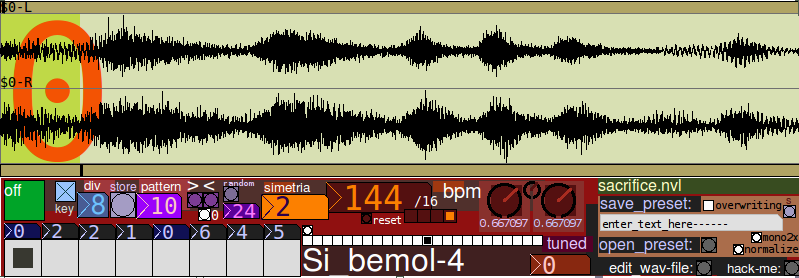
\includegraphics[scale=.6]{navalha}
% \caption{navalha}
% \label{navalha}
% \end{figure}


\begin{quote}
Este projeto é um estudo para estimular uma atividade que torna-se cada vez mais evidente no universo 
do software livre e código aberto – a customização de softwares para idéias artísticas e para produção 
multimídia em geral permitindo aquele que visa criar desenvolver suas idéias abstratas partindo de maneiras 
rápidas de trabalhar com código, ao invés da lógica onde o artista e visto como um usuário de interfaces ja 
prontas que ao tentar “prever aquilo que quer o usuário” também acaba impondo sua prática de uso. \cite{navalha}
\end{quote}

O desenvolvimento do ``Navalha'' seguiu um caminho paralelo a outros projetos coletivos, experimentos em 
execução musical e instalações. Talvez essa seja uma característica de projetos \textit{Open Source}, de que
o projeto não precisa estar ``finalizado'' para ser recombinado por outros artistas. Ambientes como o 
\textit{github}\footnote{Disponível em: www.github.com} permitem esse fluxo de código de diversos projetos
em andamento.

\begin{quote}
Com a escolha da linguagem puredata, que possui uma comunidade extremamente produtiva e colaborativa,  
por mais que esta interface esteja apresentando uma prática fechada em uma idéia de recortes de samples e um 
certo escopo, apresenta-se também como a abertura para ser recombinada com outros códigos e idéias, colocando-se 
como uma peça a ser aberta e transformada, sendo desde o início deste projeto documentada da maneira mais detalhada 
possível para permitir tal recombinação. \cite{navalha}
\end{quote}


A segunda fase da pesquisa foi o desenvolvimento do
sistema propriamente dito, com prototipação de interface para usuário,
diversos experimentos de estúdio onde cada parte do sistema foi
testada individualmente e em grupo.



%% falar mais sobre como trabalhar com software livre foi importante












%% ligar esse último parágrafo com o tema dessa introdução

%% parágrafo de conclusão



%\section{Ferramentas}

Nessa seção serão brevemente expostos os motivos pela escolha de determinadas ferramentas para
o desenvolvimento dessa pesquisa.


\section{GNU/linux}

Durante toda a pesquisa, foi usado o sistema operacional GNU/Linux.
As distribuições usadas foram Debian testing, Debian stable e Ubuntu LTS.
Muitos motivos poderiam ser listados para justificar a escolha desse sistema
operacional. Porém, gostaria de destacar a preocupação pela coerência de licenças
de uso e distribuição, entre as diversas partes que compõe a pesquisa.
O objetivo é construir programas usando componentes de software que usem as licenças GNU/GPL, ou 
BSD. O código resultante dessa pesquisa também é licenciado sob as especificações
da licença GNU/GPL.



\section{Git}

Git é um sistema de controle de versão distribuído, com código fonte livre e aberta, desenhado para lidar com qualquer
projeto, com rapidez e eficiência.
Uma grande vantagem é a facilidade de colaboração em desenvolvimento de código, onde outros desenvolvedores
podem clonar o repositório da pesquisa e realizarem "forks", ou desenvolvimentos paralelos. Isso cria uma situação 
onde o resultado da pesquisa, em termos de programação, se torna um elemento vivo dentro da comunidade de músicos e 
programadores interessados em computação musical e música interativa.

Além da possibilidade de fácil manutenção de repositórios de código local, muitas empresas oferecem serviços de
hospedagem gratuita de repositórios Git na internet. A escolha desse controle de versão se dá pelo estímulo a cooperação e 
continuidade dessa pesquisa para além do encerramento da tese, com a possibilidade de alguns resultados se proliferarem
em outros projetos de pesquisa.



\section{Jack}

JACK é um sistema para o tratamento em tempo real, áudio de baixa latência (e MIDI). 
Ele roda em GNU / Linux, Solaris, FreeBSD, OS X e Windows (e pode ser portado para outras plataformas 
POSIX-conformant). É possível conectar um número de diferentes aplicações para um dispositivo de áudio, 
bem como permitindo que eles compartilhem áudio entre si. Seus clientes podem ser executados em seus próprios 
processos (ou seja, como aplicações normais), ou podem eles podem ser executados dentro do servidor JACK 
(ou seja, como um "plugin"). JACK também tem suporte para a distribuição de processamento de áudio através de 
uma rede, tanto LANs rápido e confiável, bem como mais lento, WANs menos confiável.

\begin{figure}
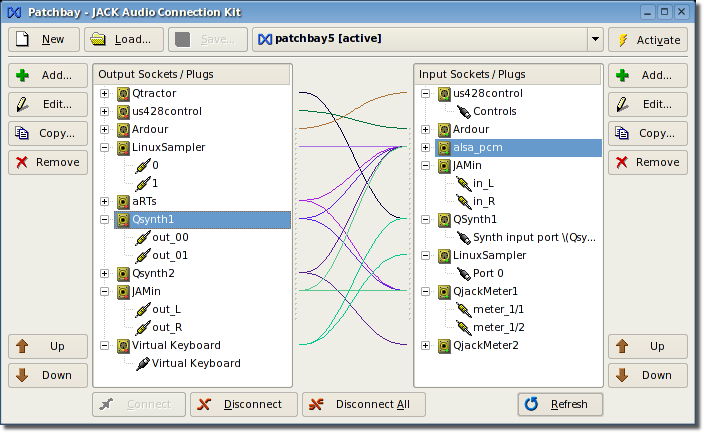
\includegraphics[scale=.7]{qjackctl}
\caption{Interface de conexão de processos do Jack}
\label{jack}
\end{figure}



\section{Rosegarden}

Rosegarden é um programa de criação e edição musical que roda em GNU/linux.
Possui diversas funcionalidades, mas nessa pesquisa é usado como sequenciador
MIDI gráfico, que recebe mensagens MIDI em tempo-real através do Jack.

A vantagem é a possibilidade de editar graficamente o resultado do diálogo entre
o áudio do instrumento convertido em MIDI e o resultado dos algoritmos dos geradores
MIDI e harmonizadores. O Rosegarden usa dois editor gráfico em formato de piano-roll
e outro em formato de notação musical. Uma sequência MIDI editada com o Rosegarden
pode ser exportada para o formato .ly, que é o formato do Lilypond.

Lilypond é uma linguagem de marcação especializada em notação musical. Segundo
a definição do próprio projeto:

\begin{quote}
 LilyPond é um programa de gravação de música, dedicada à produção a partitura da mais alta qualidade possível. 
Ele traz a estética da música tradicional escrita para impressões de computador. LilyPond é software livre e 
parte do Projeto GNU.
\end{quote} 

O Rosegarden executa as sequências MIDI usando um servidor de arquivos soundfont.
Um arquivo SoundFont, ou "banco" SoundFont, contém uma ou mais amostras de áudio de onda (ou "amostras"),
que pode ser re-sintetizados em alturas diferentes e níveis dinâmicos. Cada forma de onda amostrada pode ser
associado a um ou mais intervalos de notas e dinâmica. De modo geral, a qualidade de um
SoundFont banco é uma função da qualidade das amostras de digitais e da associação inteligente
de amostras com as séries do campo apropriado. A qualidade da soundfont também depende do número de amostras
tomadas por um determinado intervalo de notas. 



\section{Pd-extended}

O Pure data(Pd), foi a linguagem escolhida para o desenvolvimento dessa pesquisa.
Existem diversas distribuições do Pd, sendo as mais utilizadas o Pd "vanilla" e o Pd-extended.
A versão "vanilla" se refere ao núcleo da linguagem mantida pelo criador Miller Puckette, e no
momento de escrita dessa tese se encontra na versão 0.43. Já o Pd-extended conta com as contribuições
da comunidade de desenvolvedores e usuários, que incluíram diversas extensões para vídeo, gráficos, rede e
novas funcionalidades para criação musical.

No atual momento, essa pesquisa depende do Pd-extended, porém, para o desenvolvimento futuro pretende-se
que as abstrações dependam, apenas da versão vanilla. A desvantagem de usar a distribuição Pd-extended é quebraa mesma 
depende de muitos outros componentes de software, tornando uma possível compatibilidade da pesquisa com sistemas
futuros um pouco mais arriscada. 


\section{Bibliotecas de Pd}

Além do Pd-extended, essa pesquisa, necessita de duas outras bibliotecas, sendo elas a PDMTL e DIY2.

Também são usados os objetos compilados em C, desenvolvidos por William Brent:

\begin{itemize}
 \item tabletools
 \item timbreID
\end{itemize}


%\begin{figure}
%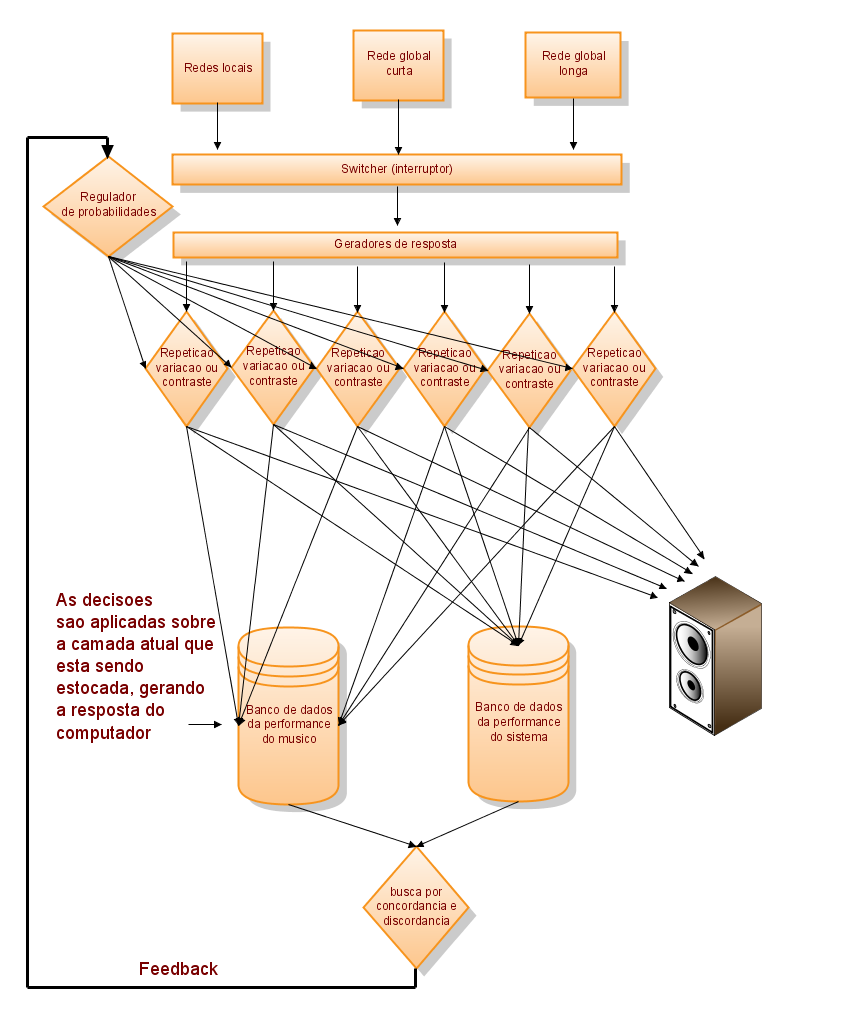
\includegraphics[scale=.6]{mecanismo}
%\caption{Mecanismo de decisões e geração de resposta}
%\label{mecanismo}
%\end{figure}










\newpage






\chapter{SInCoPA}
\label{chap:SInCoPA}


Na teoria musical, a síncopa é uma característica rítmica caracterizada pela execução de som em um tempo fraco, 
ou parte fraca de tempo sendo prolongado até o tempo forte, criando um deslocamento da acentuação rítmica. 
Além de SInCoPA ser a abreviação de Sistema Interativo de Composição Performance e Análise, o termo se encaixa
no sentido poético dessa pesquisa. Como uma metáfora, significando a busca de um gesto musical não determinado pela notação
ou por uma pré-configuração de software que determine de forma dominante a narrativa musical.

  Nesse capítulo serão expostas as abstrações desenvolvidas para o sistema, como também
os protótipos e programas auxiliares desenvolvidos para explicar o uso correto das 
abstrações apresentadas. O conjunto de abstrações cumpre funções básicas necessárias
a projetos de música interativa que relacionem análise de áudio e geradores musicais
baseados nos dados da análise do áudio de entrada em tempo-real. Como é um sistema 
em contínuo desenvolvimento, muitos patchs mostrados apresentam experimentos ou apontam
elementos e idéias para futuras implementações.

  Foi desenvolvida uma biblioteca de funções utilitárias em forma de abstrações, 
tornando fácil seu re-uso em outros projetos. As abstrações se dividem em 7 categorias:

\begin{enumerate}
 \item Análise de áudio de entrada em tempo-real;
 \item Geradores MIDI baseados no comportamento do áudio de 
entrada, com variações de controle, indo da mímese do sinal de entrada
até um grau mais elevado de contraste rítmico e melódico;
 \item Geradores de síntese sonora, também baseados no comportamento
do áudio de entrada com diversos níveis de controle;
 \item Módulos de processamento de sinal, usados no áudio de entrada e no
áudio gerado pela comunicação MIDI;
 \item Visualizador de notação musical do áudio de entrada e de saída;
 \item Cenários de comportamentos interativos e Mixer de volumes responsivo;
 
\end{enumerate}

Algumas abstrações são maiores e com funcionalidade mais geral, enquanto
que outras são bem menores e mais específicas.
Uma composição musical utilizando SInCoPA, consiste na concatenação de
regras que coordenam os comportamentos das várias partes envolvidas.
Esse conjunto de regras foi denominado de ``cenário''. Na composição
de um cenário o compositor escolhe, por exemplo,  se determinado gerador 
deve ter um comportamento complementar ou contrastante  em relação a algum
parâmetro de análise.



%% testar esse novo teclado - falar sobre o controlador pedal 

%% aqui pra cada patch um formato de projeto:
%% intro + objetivo + justificativa + metodologia+ conclusão e desenvolvimento futuro


%%\subsection{Biblioteca de Utilitários}



\section{Análise de áudio}

\begin{figure}
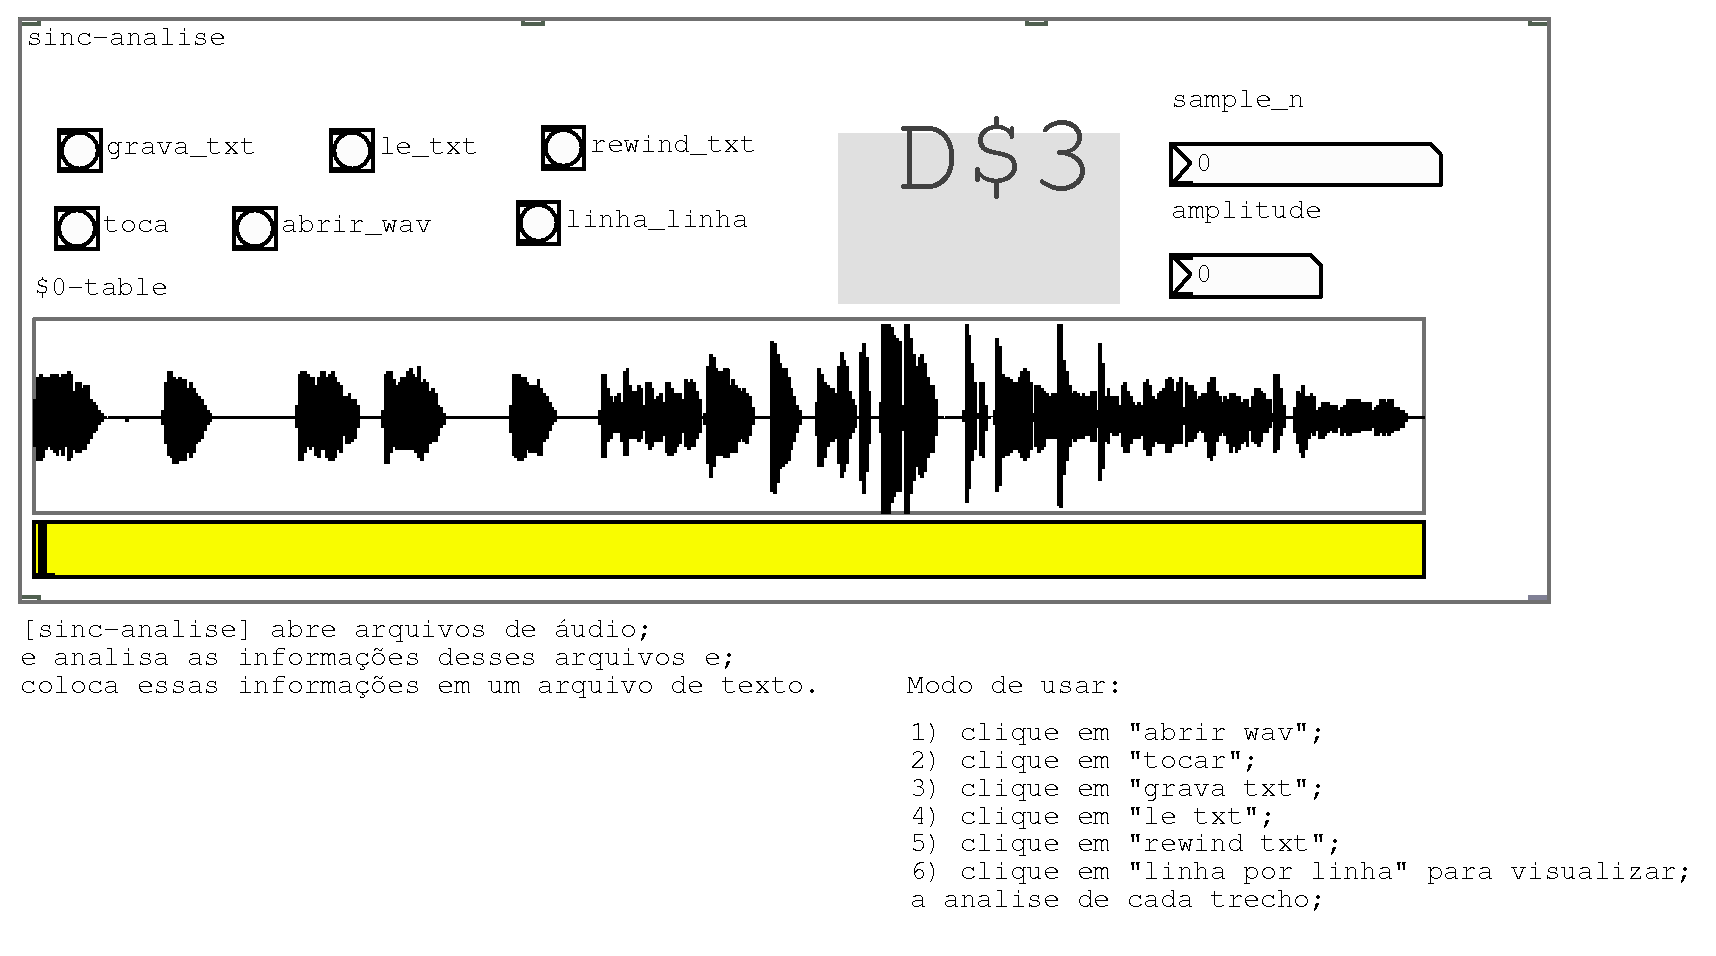
\includegraphics[scale=.6]{sinc-analise}
\caption{Objeto de análise de áudio [sinc-analise]}
\label{sinc-analise}
\end{figure}


Nessa seção serão apresentados os problemas e soluções específicos
a análise de áudio. 

É importante a flexibilização para a detecção de parâmetros musicais.
Também é importante a possibilidade de salvar os dados das análises serem
destacados nas interfaces dos objetos.

A interface gráfica dos objetos prevê visualização em tempo-real
da atividade no módulo de análise e botões descritos para controle
de parâmetros diversos.

Um dos primeiros objetos desenevolvidos para análise é o [sinc-analise],
mostrado na figura \ref{sinc-analise} que faz análise de fundamental e amplitude
de ataque de cada nota. Esses dois parâmetros são colocados em uma lista, juntamente com a indicação
de qual sample (localização) a lista se refere e são salvos em um arquivo de texto.



\subsection{Entrada de áudio}

Um elemento importante na interface é a visualização instantânea
do fluxo de áudio. Aqui na figura \ref{audioin} apresentamos uma solução prática e podemos
ver uma outra abordagem na figura \ref{sinc-fft} baseada em análise FFT.

\subsubsection{Objeto [sinc-audioin]}


\begin{figure}
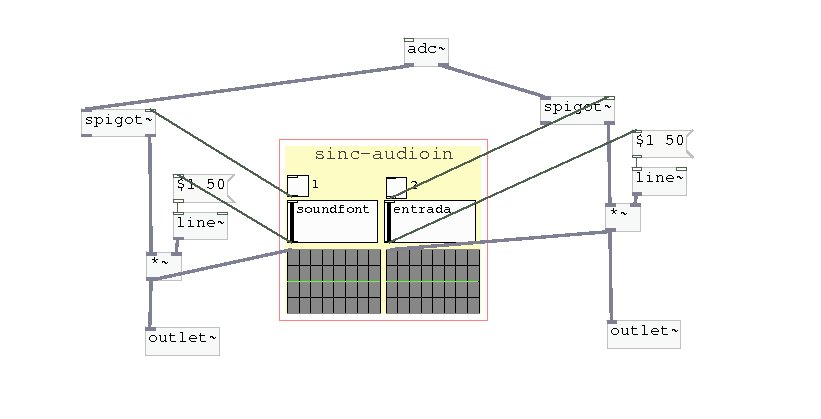
\includegraphics[scale=.55]{audioin}
\caption{Entrada de áudio [sinc-audioin]}
\label{audioin}
\end{figure}

A entrada de áudio no pd começa com o objeto  [adc\texttildelow], e sempre segue um fluxo
básico que passa por um objeto de multiplicação de sinal [*\texttildelow] que permite um
controle manual de entrada de áudio. Esse controle é necessário para ajustar 
a sensibilidade dos objetos que realizarão a análise de áudio. A abstração 
[sinc-audioin] na figura \ref{audioin} permite o roteamento e visualização rápida 
de entrada de áudio de dois canais. No caso dos experimentos musicais envolvidos 
nessa pesquisa, foi estabelecido o canal 1 para o recebimento de áudio do programa 
rosegarden, que hospeda samplers do tipo \textit{soundfont}. O canal 2 é usado para 
a entrada de áudio do instrumento. É necessário um objeto que funcione como uma chave de
liga/desliga para o áudio. Para isso foi usado o objeto [spigot\texttildelow] da biblioteca
\textit{Unauthorized} incluída no pd-extended.
 Quando o toggle([tgl]) é acionado com clique de mouse,
ele envia o valor 1 pela saída que por sua vez está conectado na entrada fria do
[spigot\texttildelow], essa ação faz com que o áudio seja liberado pela saída do [spigot\texttildelow].
Os volumes de entrada são controlados por objetos gráficos sliders ([hsl]), que tem
a saída ligada a uma variável de parâmetro para o objeto [line\texttildelow]. Nesse caso específico
[line\texttildelow] atua no sentido de se evitar cliques no áudio quando se muda o valor de 
amplitude que entra na entrada fria do objeto [*\texttildelow]. Outro componente
opcional, que é útil em situações práticas, é um visualizador gráfico de presença de sinal
de áudio. Em [sinc-audioin] é usado o objeto [Scope\texttildelow] da biblioteca \textit{cyclone}, 
incluída no pd-extended.

%% dar uma olhada no livro do Miller sobre [*~] e [line~] 

\subsubsection{Objeto [sinc-fft]}

%% fazer a figura do patch

\begin{figure}
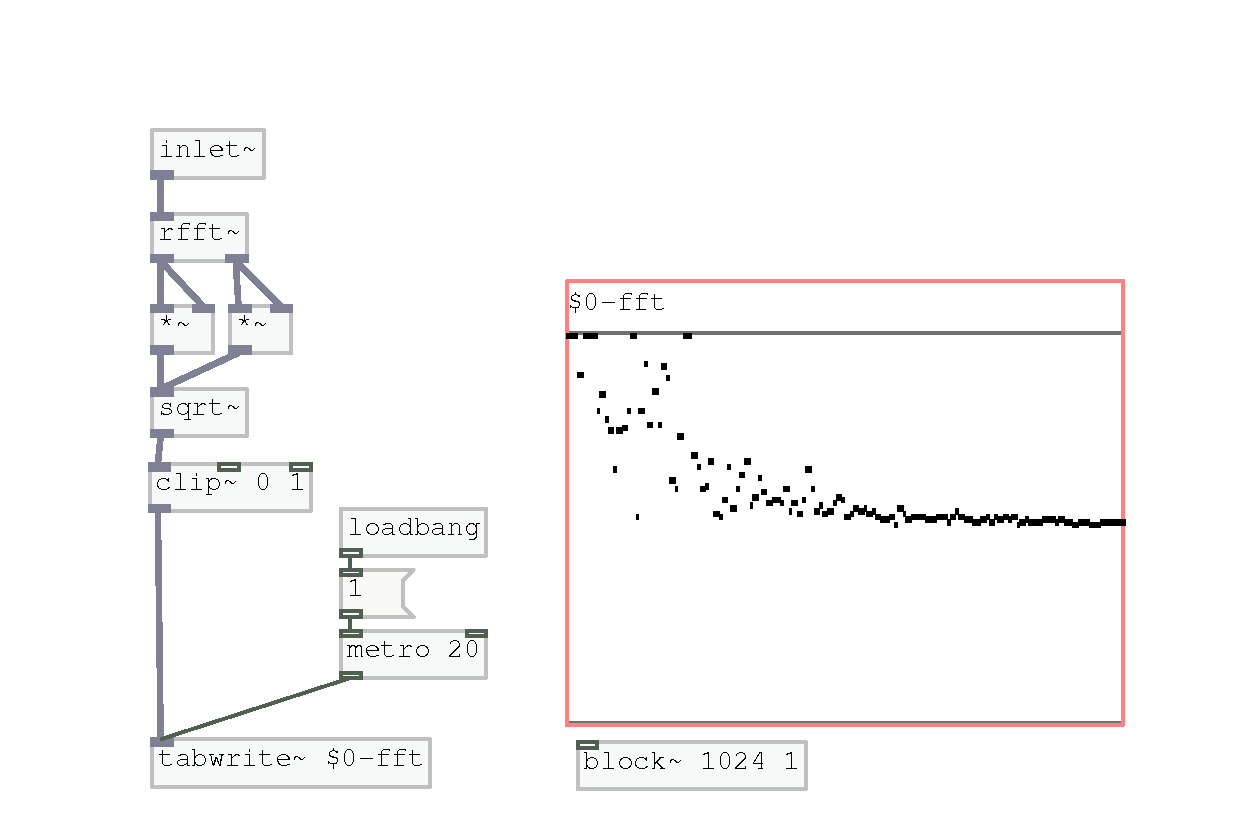
\includegraphics[scale=.55]{sinc-fft}
\caption{Visão interna de [sinc-fft]}
\label{sinc-fft}
\end{figure}



A abstração [sinc-fft] mostra graficamente uma janela de análise FFT com bloco de amostragem
definido por [block\texttildelow] em 1024. O que significa que o objeto [rfft\texttildelow],
irá retornar valores encontrados de amplitude e fase para 512 frequências múltiplas de 43 Hz.
Que é a frequência resultado da taxa de amostragem (44100) dividida pelo tamanho do bloco (1024).

A amplitude de cada parcial é retornada em pares reais e imaginários descritos em coordenadas
polares. Podemos calcular as amplitudes convertendo as coordenadas do sistema polar para cartesiano 
através da raiz quadrada aplicada
a soma do valor real e imaginário elevados, cada um, a própria potência. Isso pode ser feito no Pd com os
objetos [*\texttildelow] localizados abaixo de [rfft\texttildelow] realizando a potência e enviando o resultado 
simultaneamente para o objeto [sqrt\texttildelow] que opera a raiz quadrada.

O objeto [clip\texttildelow], com os argumentos 0 e 1 apenas filtra os valores negativos para uma
melhor visualização gráfica.

\begin{figure}
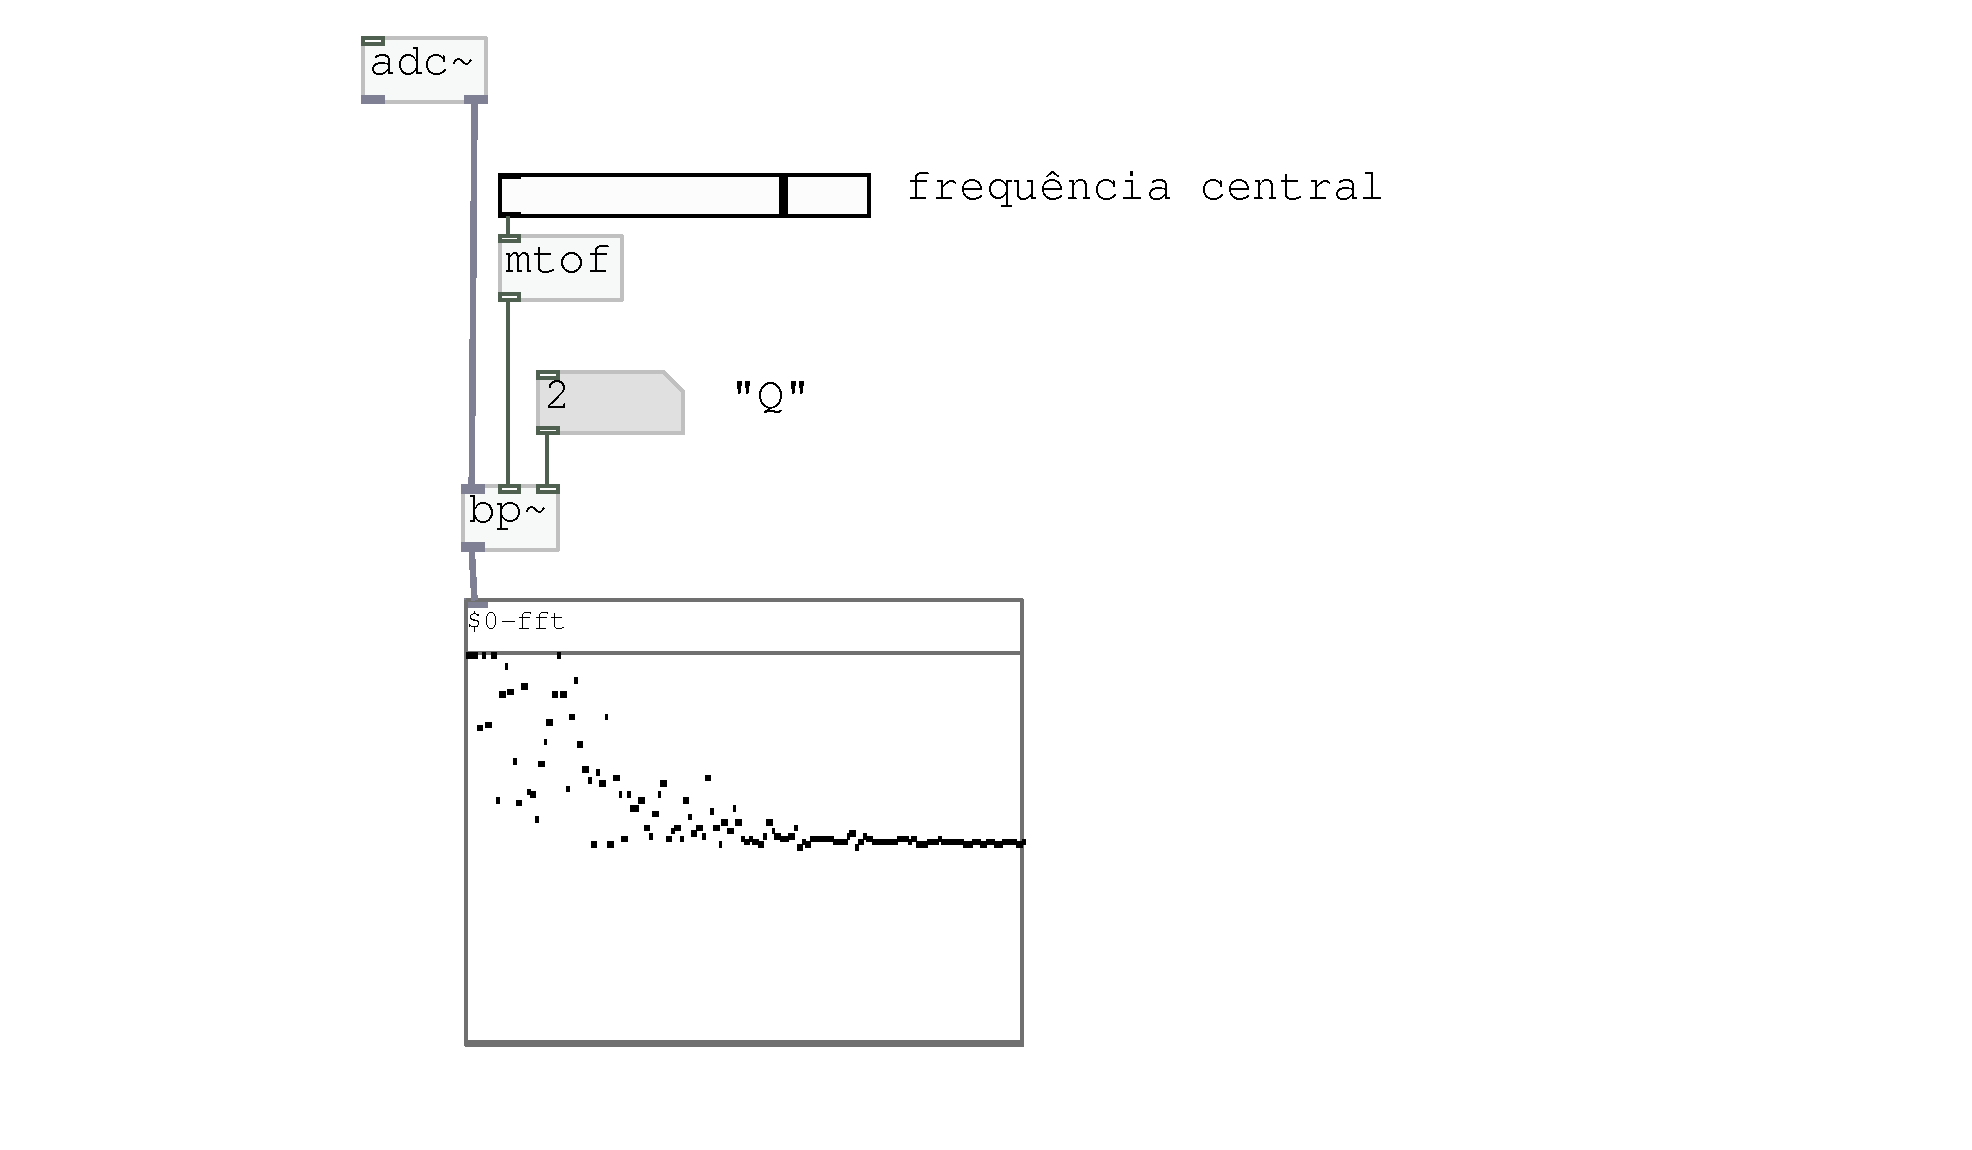
\includegraphics[scale=.55]{sinc-fft-help}
\caption{Exemplo de uso de [sinc-fft]}
\label{sinc-fft-help}
\end{figure}


A presente abstração é muito útil em situações de filtragem de entrada de áudio em tempo-real, principalmente
quando utilizados microfones condensadores que são muito sensíveis.
A visualização da análise FFT no array permite que se tenha uma boa medida na parametrização de filtros.
Como é o caso do exemplo na figura \ref{sinc-fft-help}. Onde a entrada de áudio passa por um filtro
de áudio [bp\texttildelow]. O filtro implementado em [bp\texttildelow] deixa passar uma senóide ao
redor da frequência central enquanto as outras frequências são atenuadas de acordo com o fator ``Q''
\footnote{Para uma explicação completa sobre o fator Q : http://en.wikipedia.org/wiki/Q-factor} .
Na entrada da esquerda entra o sinal de áudio, na entrada do meio é definida a frequência central e na
entrada da direita se controla o fator ``Q''. O resultado da filtragem é enviada para [sinc-fft] onde 
pode-se ter uma maior precisão na filtragem através da comparação gráfica.

 

\subsection{Manipulação de amostras}


  Dentro do  contexto de laboratório de prototipação, se faz necessário emular uma entrada 
de áudio em tempo-real com a execução de trechos de áudio sampleados ou um sintetizador simples
com entrada de notas pelo teclado alfa-numérico do computador. Nesse sentido foram construídas
algumas abstrações para facilitar o processo de desenvolvimento e teste.

\subsubsection{Objeto [sinc-sample]}



\begin{figure}
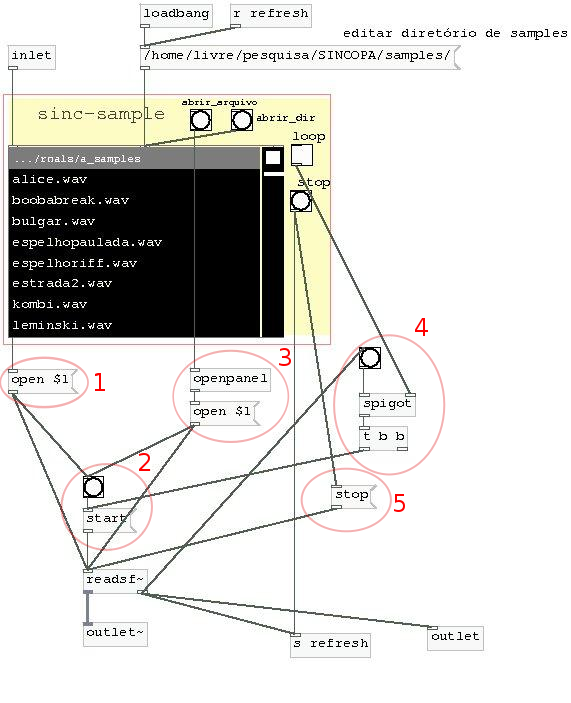
\includegraphics[scale=.5]{sinc-sample}
\caption{[sinc-sample]}
\label{[sinc-sample]}
\end{figure}



A primeira a ser desenvolvida foi a abstração [sinc-sample] mostrado na figura
\ref{[sinc-sample]}. Para essa abstração foi escolhida a abstração gráfica 
[file.browser] 
na área 1 circulada na figura \ref{[sinc-sample]} que lê os arquivos de determinado
 diretório e lista eles graficamente possibilitando que
o usuário clique no nome do arquivo escolhido, resultando em uma mensagem com a 
localização
do arquivo. Essa abstração faz parte do pacote ``pdmtl'' de abstrações de pd.
A execução do áudio é feita com o objeto [readsf\texttildelow] que precisa de três mensagens:
start, stop e localização do arquivo. O mecanismo grifado na área 2, mostra
um objeto [trigger]([t]) realizando uma tarefa em 3 fases da direita para a esquerda:
\begin{itemize}
 \item Aciona a mensagem com o caminho do arquivo a ser tocado
 \item Aciona a mensagem ``start''
 \item Recarrega a mensagem que atualiza o diretório a ser lido por [file.browser]
\end{itemize}

Outro aspecto dessa abstração é a possibilidade de tocar um arquivo de áudio em loop.
Na área circulada 4 temos um [spigot] que atua como interruptor de um bang enviado pela
saída direita de [readsf\texttildelow], que por sua vez é enviado quando [readsf\texttildelow] 
acaba de ler o arquivo
inteiro. Se o toggle que está conectado com o [spigot] da área 4 estiver ligado, ele permite
que o bang enviado ao final da leitura seja roteado para outro objeto trigger que aciona as 
duas primeiras fases descritas acima, realizando uma leitura contínua do arquivo de áudio
escolhido.



\subsection{Análise melódica}


Existem diversos problemas de pesquisa relacionados com a
análise melódica como por exemplo:

\begin{itemize}
 \item Detecção de notas;
 \item Estimativa de nota;
 \item Conversão de fluxo de áudio em dados semânticos (MIDI);
 \item Permeabilidade melódica;
 \item Análise de contorno e direcionamento melódico;
\end{itemize}




\subsubsection{Objeto [sinc-audioanalise]}

Um dos fatores mais importantes para a prática de análise melódica
em tempo real é a flexibilidade de refinamento dos parâmetros
de análise. Esses parâmetros devem estar ao alcance rápido e documentados
e sinalizados na interface.

O objetivo é reunir num só módulo, a detecção de ataques de notas 
(baseado no objeto [bonk\texttildelow]) com a análise de frequências
baseada no objeto [sigmund\texttildelow], e ainda ligando o resultado das 
análises com objetos de conversão MIDI.

%% não seria o caso separar: [sinc-audioanalise] -> [sinc-audio2midi] -> [sinc-analisemelodica]

Nessa abstração procurou-se desenvolver uma interface que facilite
a rápida prototipação e flexibilidade de parâmetros que podem
se adaptar facilmente para diferentes fontes sonoras.

\begin{figure}
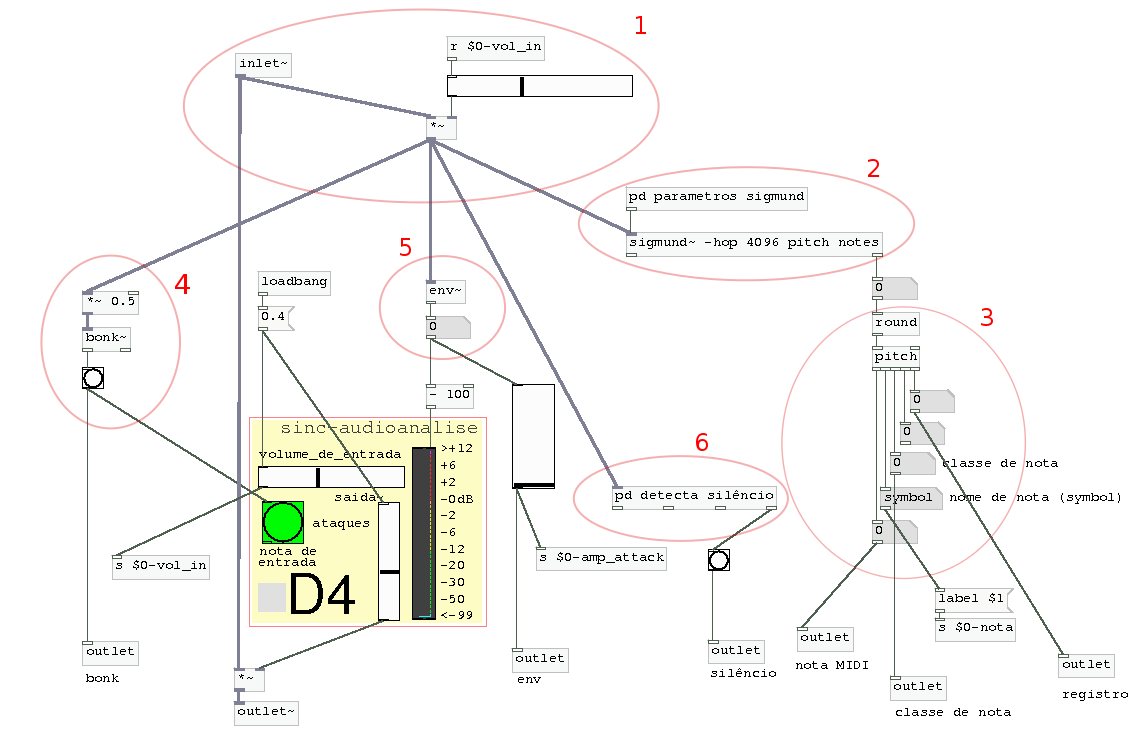
\includegraphics[scale=.4]{sinc-audioanalise}
\caption{[sinc-audioanalise]}
\label{[sinc-audioanalise]}
\end{figure}

Como podemos ver na área 1 da figura \ref{[sinc-audioanalise]},
temos o controle de um slider vertical\footnote{objeto [hslider]}
controlando a amplitude geral do áudio de entrada. Esse controle
é muito importante em situações em que se tem variações de amplificação
entre ensaios e performance.

%%Área 1: explicação da amplificação de volume de entrada/volume de saída

\begin{figure}
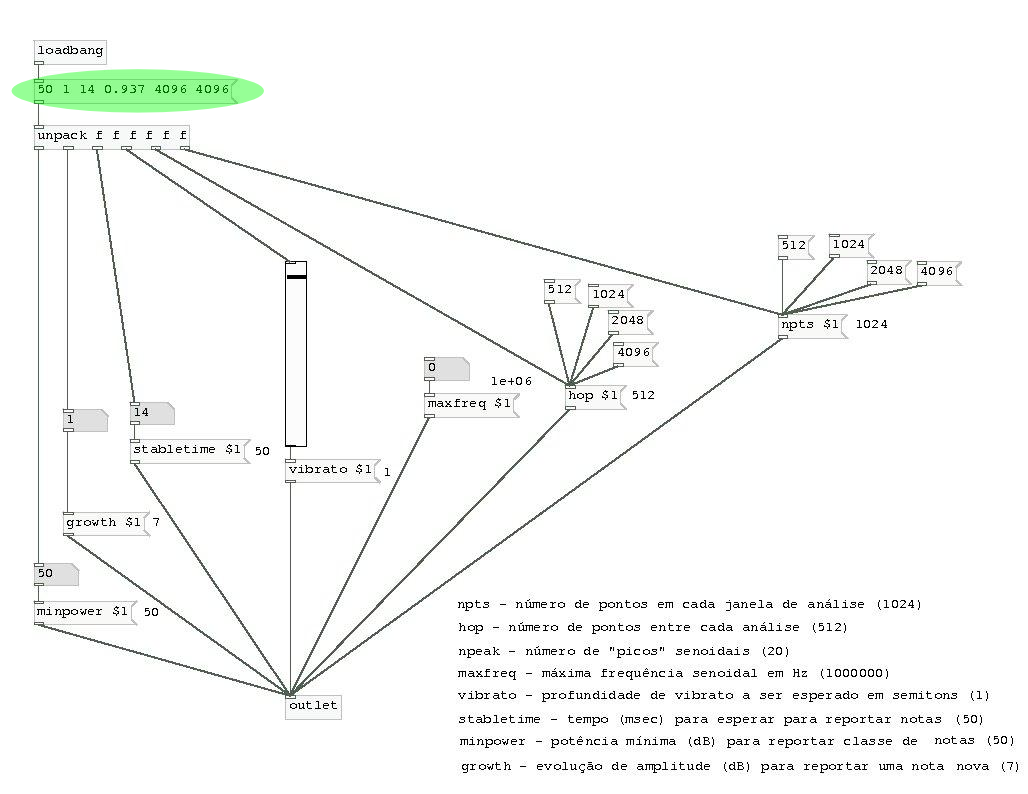
\includegraphics[scale=.5]{sinc-audioanalise-param}
\caption{sub-patch que controla as configurações de [sigmund\texttildelow]}
\label{[sinc-audioanalise-param]}
\end{figure}


Na área 2 aparece um subpatch que pode ser visto na figura
\ref{[sinc-audioanalise-param]}. Nesse subpatch podemos ver 
a organização dos parâmetros do objeto [sigmund\texttildelow].

O objeto [sigmund\texttildelow] faz análise de áudio no domínio da 
frequência e detecção de notas. Os parâmetros podem ser re-definidos
em tempo-real através dos argumentos de criação do objeto ou através
de mensagens como é o caso aqui.


Segundo a documentação no próprio manual do objeto:
\begin{quote}
 Sigmund\texttildelow analisa um áudio de entrada através de componentes senoidais,
que podem ser retornados individualmente ou combinados para
retornar uma estimativa de altura. Saídas possíveis são especificadas
como argumentos de criação:

\begin{itemize}
 \item pitch - saída constante
 \item notes - retorna a altura no começo das notas 
 \item env - retorna amplitude continuamente
 \item peaks - retorna todos picos senoidais em ordem de amplitude
 \item tracks - retorna picos senoidais organizados em faixas separadas
\end{itemize}

Parâmetros que você pode definir (no argumentos de criação do objeto ou em mensagens):

\begin{itemize}
 \item npts - número de pontos em cada janela de análise (1024)
 \item hop - número de pontos entre cada análise (512)
 \item npeak - número de picos senoidais (20)
 \item maxfreak - máxima frequência senoidal em Hz. (1000000)
 \item vibrato - profundidade de vibrato a ser esperado em semitons (1)
 \item stabletime - tempo (mseg) para esperar para reportar notas (50)
 \item minpower - mínima amplitude (dB) para retornar uma altura (50)
 \item growth - crescimento de amplitude (dB) para retornar uma nova nota (7) 
\end{itemize}
Os parâmetros npts e hop são em número de amostras, e são definidos como potências de dois.\footnote{

 Sigmund\texttildelow analyzes an incoming sound into sinusoidal
components, which may be reported individually or combined to
form a pitch estimate. Possible outputs are specified as creation
arguments:

\begin{itemize}
 \item pitch - output continuously
 \item notes - output pitch at the beginning of notes
 \item env - output amplitude continuously
 \item peaks - output all sinusoidal peaks in order of amplitude
 \item tracks - output sinusoidal peaks organized into tracks
\end{itemize}
Parameters you may set (in cretaion arguments or messages):

\begin{itemize}
 \item npts - number of points in each analysis window (1024)
 \item hop - number of points between each analysis (512)
 \item npeak - number of sinusoidal peaks (20)
 \item maxfreak - maximum sinusoid frequency in Hz. (1000000)
 \item vibrato - depth of vibrato to expect in 1/2 tones (1)
 \item stabletime - time (msec) to wait to report notes (50)
 \item minpower - minimum power (dB) to report a pitch (50)
 \item growth - growth (dB) to repor a new note (7) 
\end{itemize}
The npts and hop parameters are in samples. and are powers of two.}
\end{quote} 


\begin{figure}
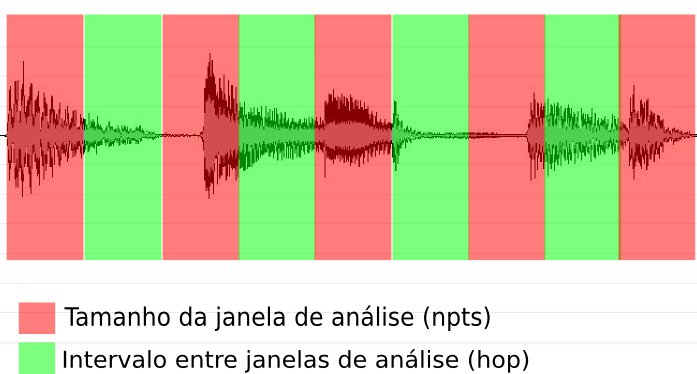
\includegraphics[scale=.7]{sigmund}
\caption{Tamanho de janela de análise (npts)}
\label{janela-analise}
\end{figure}


Nesse caso optou-se por pré-inicializar [sigmund\texttildelow] com as
opções : "-hop 4096 pitch notes" . Através de testes empíricos preferiu-se
usar apenas a saída de "notes" por apresentar uma saída mais precisa para notas 
musicais. A mensagem em destaque na figura \ref{[sinc-audioanalise-param]} representa
a inicialização dos valores de todos parâmetros de [sigmund\texttildelow].

Os principais parâmetros definem o tamanho da janela de análise.
Nesse caso "npts" e "hop" tem uma relação direta
por se tratar do tamanho da janela de análise e o espaço
entre as janelas em samples como pode ser visto na figura \ref{janela-analise}.



%%Área 2: explicação do sigmund~ - ver livro Miller + help do sigmund~


\begin{figure}
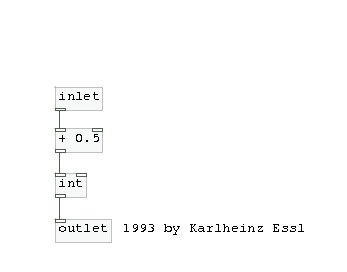
\includegraphics[scale=.7]{round}
\caption{[round]}
\label{round}
\end{figure}


Na área 3 vemos o objeto [round], presente na biblioteca RTC, responsável
por arredondar o valor de entrada para cima. O arredondamento é feito com
a soma de 0.5 e transformação do número do tipo float para tipo inteiro ([int]),
como pode ser visto na figura \ref{round}.


\begin{figure}
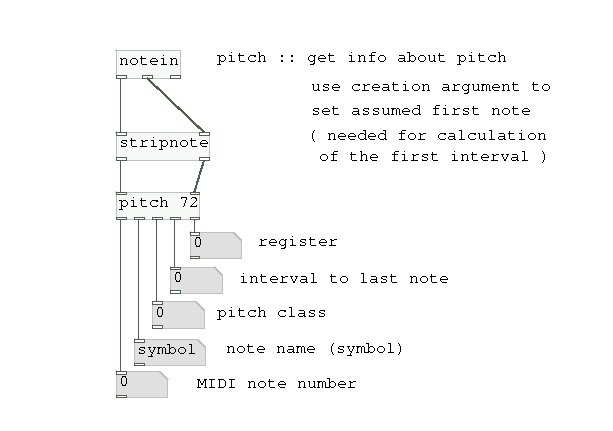
\includegraphics[scale=.7]{pitch}
\caption{[pitch]}
\label{pitch}
\end{figure}


\begin{figure}
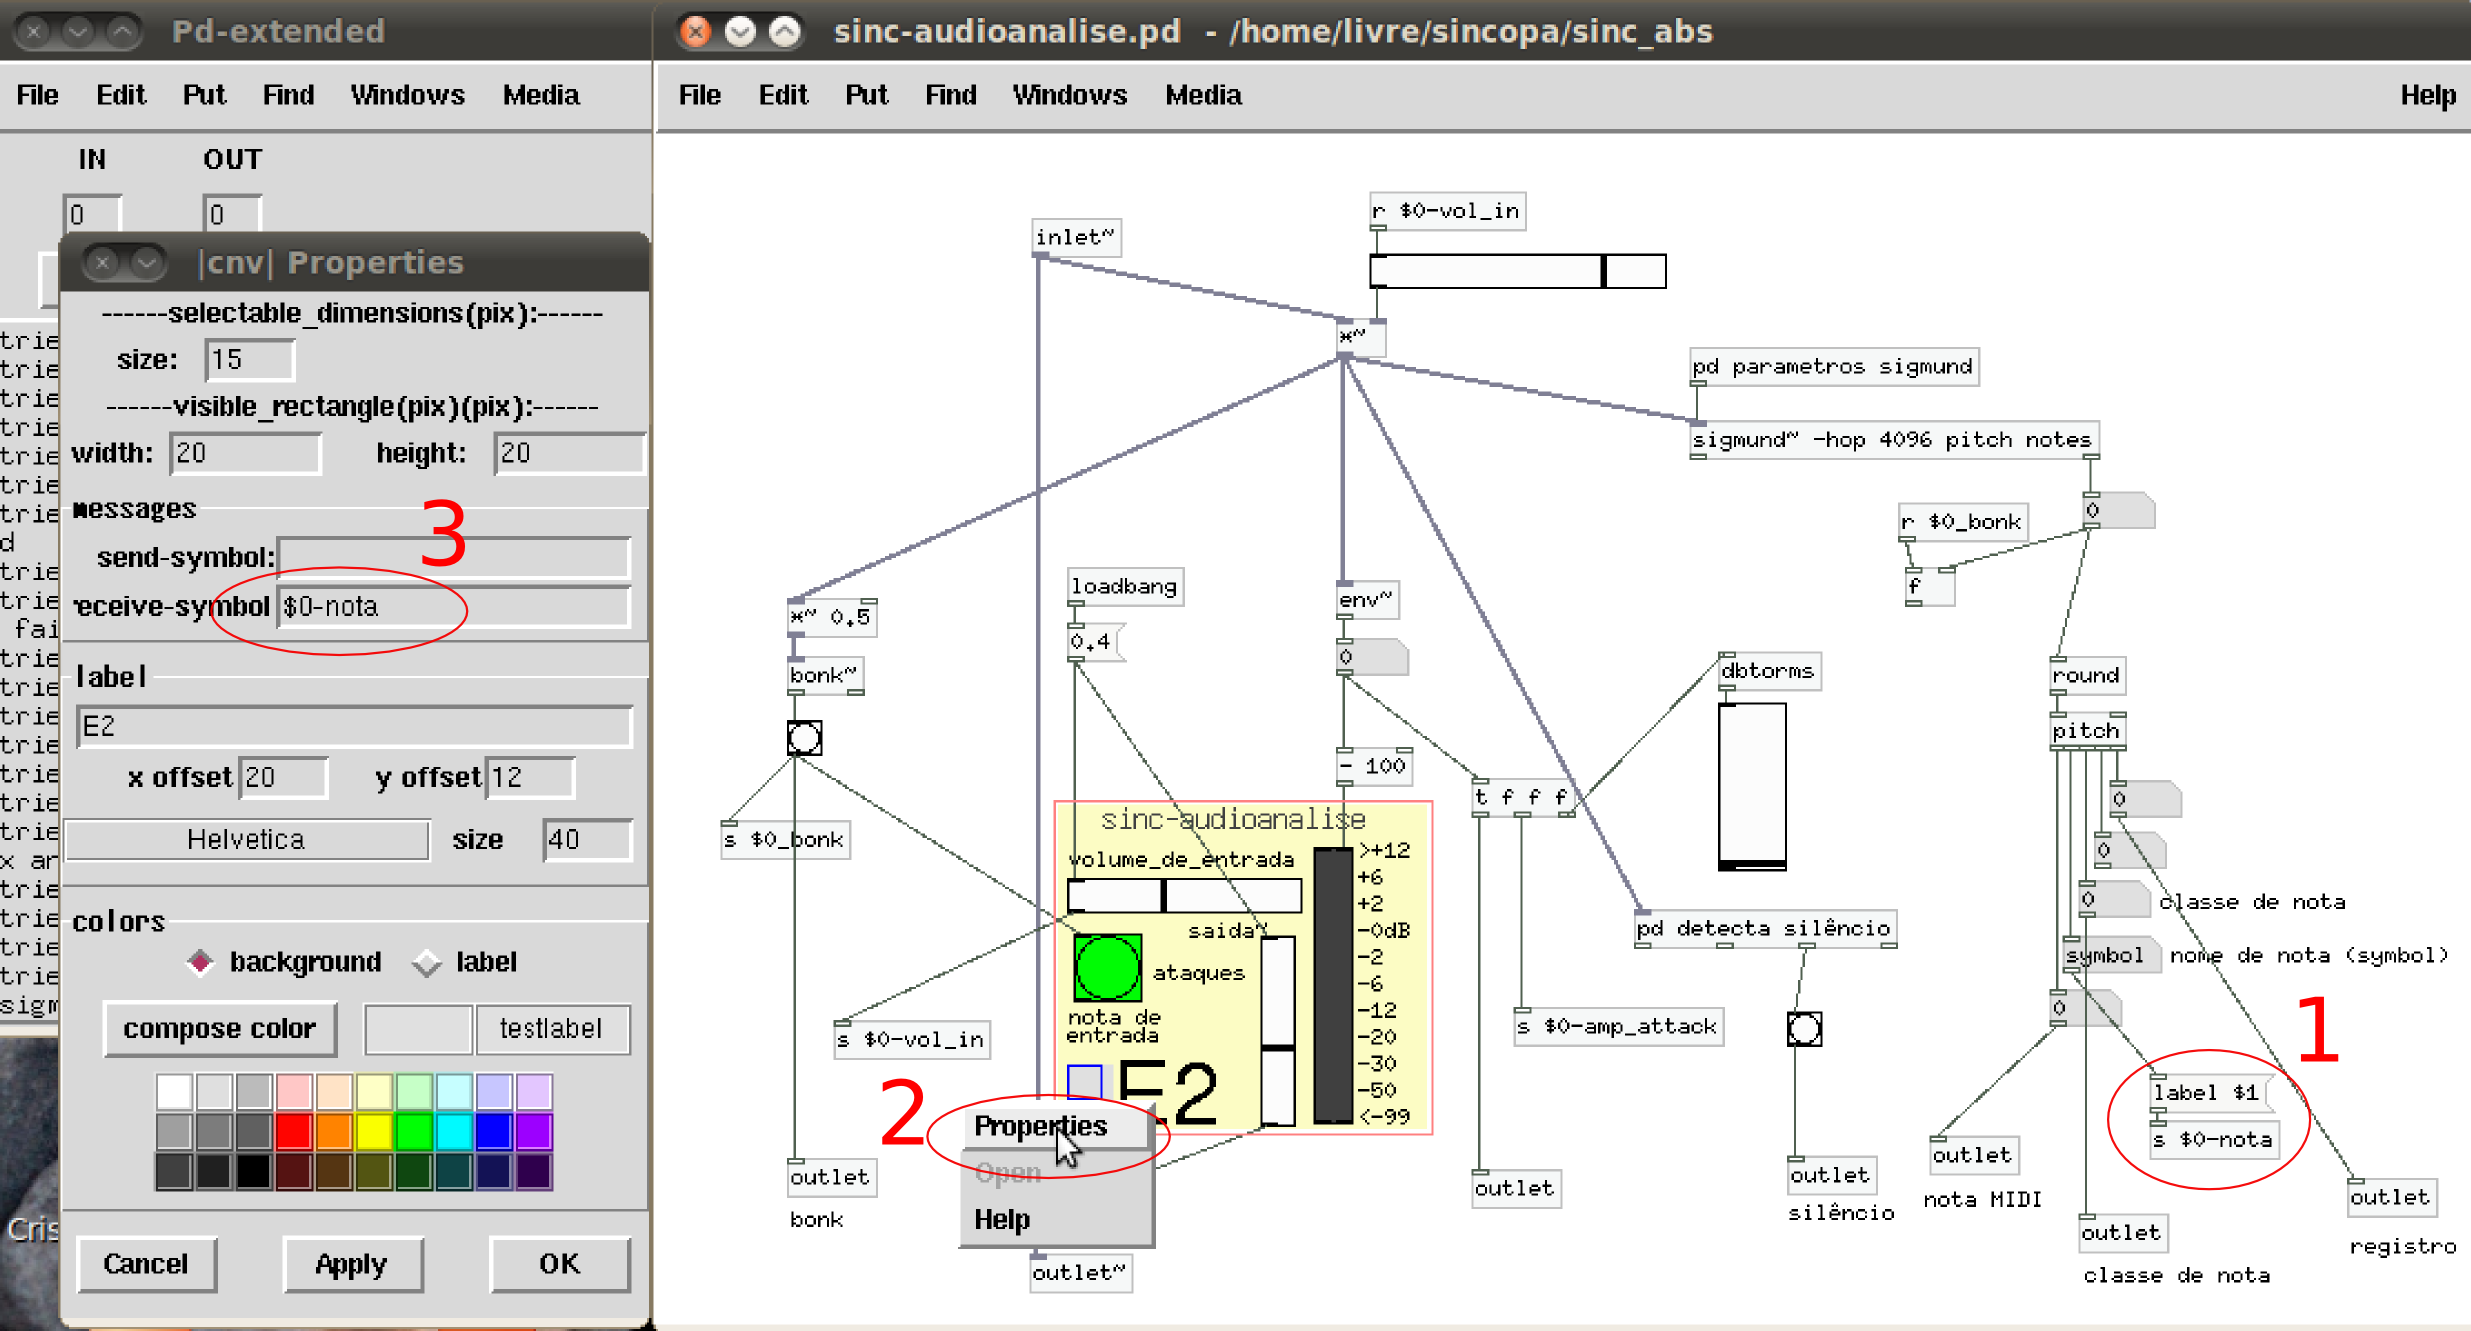
\includegraphics[scale=.5]{canvas-edit}
\caption{editando objeto canvas ([cnv])}
\label{canvas-edit}
\end{figure}


O objeto [pitch] pertence a biblioteca maxlib, distribuída junto com o 
pd-extended e sua funcionalidade pode ser vista no próprio help do objeto na 
figura \ref{pitch}. A interface gráfica de [sinc-audioanalise] mostra o pitch
da nota detectada em tempo-real. A visualização é feita com o objeto canvas ([cnv]).
A segunda saída do objeto [pitch] retorna um símbolo com a cifra e oitava
da nota. Esse símbolo é enviado para o canvas com o método "label" através
da variável \$0-nota. O objeto canvas aceita variáveis enviadas com o objeto [send],
editando as propriedades do canvas (ver figura \ref{canvas-edit}). A visualização em tempo-real
é indispensável para calibrar a análise de áudio.


%%Área 3: explicação de round e pitch + plotar cifra no canvas


Na área 4 vemos o objeto [bonk\texttildelow], desenvolvido para
detectar ataques de notas. Segundo Puckette:

%% biblio: Miller (Real-time audio analysis tools for Pd and MSP) - 98
\begin{quote}
O objecto bonk faz filtragem com limite \textit{Q} de um som de entrada e
pode produzir a análise crua ou detectar inícios
que pode então ser comparado com um conjunto de modelos espectrais conhecidos
a fim de adivinhar qual dos vários
tipos possíveis de ataque que ocorreu.

Os objetos fiddle e bonk são de baixa tecnologia, seria fácil para re-escrever os
algoritmos  em outra linguagem
 ou ambiente. Nossa principal preocupação é atingir comportamento aceitável e previsível e
 o usando técnicas fáceis de entender que não vão exigir uma carga computacional inaceitável
 em um computador moderno\footnote{The bonk object does a bounded-Q fillterbank of an incoming sound and
can either output the raw analysis or detect onsets
which can then be compared to a collection of known
spectral templates in order to guess which of several
possible kinds of attack has occurred.

The fiddle and bonk objects are low tech; the
algorithms would be easy to re-code in another lan-
guage or for other environments from the ones consid-
ered here. Our main concern is to get predictable and
acceptable behavior using easy-to-understand tech-
niques which won't place an unacceptable computa-
tional load on a late-model computer.}. \cite{bonk}
 
\end{quote}

\begin{figure}
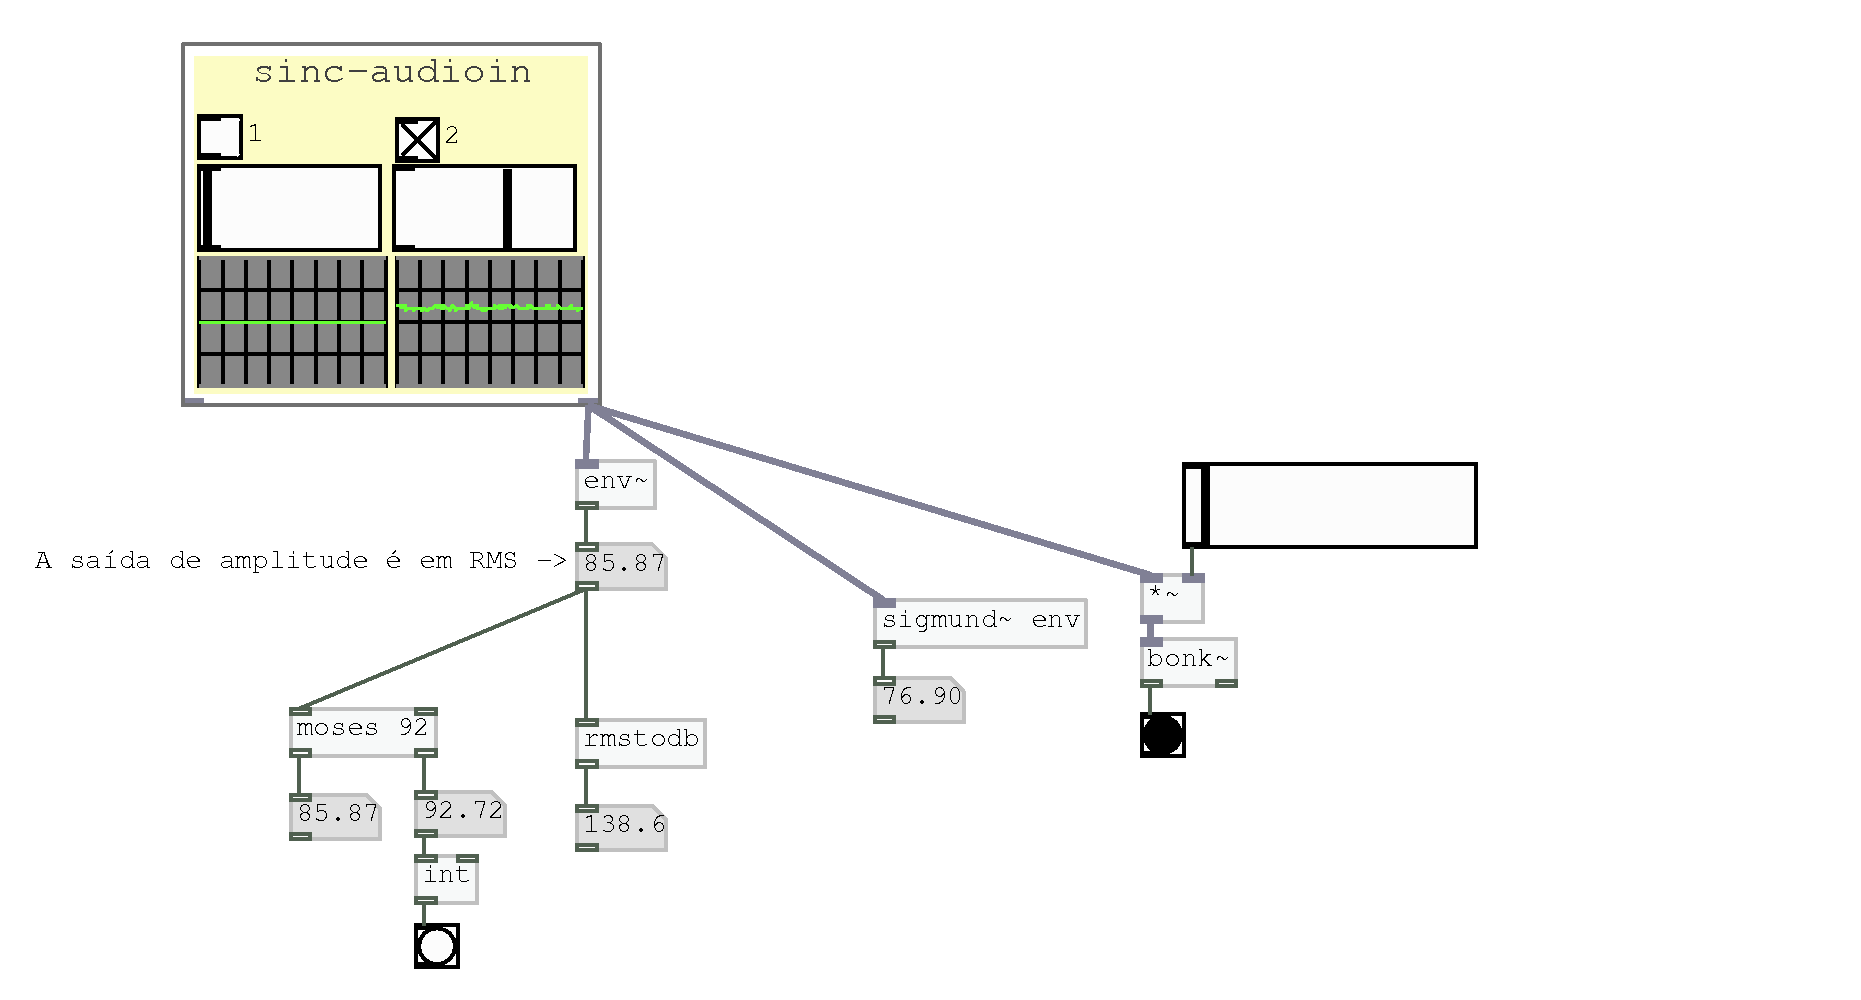
\includegraphics[scale=.5]{bonks}
\caption{Métodos de análise de amplitude}
\label{bonks} 
\end{figure}


No Pd, outros objetos possibilitam a análise da amplitude,
na figura \ref{bonks} vemos 3 métodos. O objeto [env\texttildelow]
retorna o valor de amplitude de um sinal em RMS. O objeto
[sigmund\texttildelow] pode mapear a amplitude com a opção
"env".


Ainda Puckette, aponta as vantagens de usar [bonk\texttildelow]
em vez de outros métodos.

\begin{quote}
A aplicação mais satisfatória desta análise está na
detecção de ataques de percussão. A forma mais popular
de fazer isso é usar um analisador de envelope e olhar
para o rápido aumento na amplitude, mas qualquer tipo de
toque pode definir sequências de ataques indesejados, ou ao contrário, 
pode mascarar ataques verdadeiros. A análise utilizada por
bonk muitas vezes pode detectar ataques novos que aparecem como
afiadas mudanças relativas no espectro sem qualquer
acompanhamento na mudança na amplitude global; reciprocamente, 
os instrumentos musicais não costumam mudar o espectro rapidamente
e, portanto, não atraem a atenção de bonk\footnote
{The most satisfying application of this analysis is in
detecting percussive attacks. The most popular way
of doing this is to use an envelope follower and look
for rapid rises in follower output; but any kind of
ringing can set o trains of unwanted attacks, or op-
positely, can mask true attacks. The analysis used by
bonk can often detect new attacks which appear as
sharp relative changes in the spectrum without any
accompanying large change in the overall power; con-
versely, ringing instruments don't often give rapidly
changing spectra and hence don't attract bonk's at-
tention.}. \cite{bonk}
\end{quote}

A biblioteca Aubio de Paul Brossier também contém um objeto
especializado em detectar ataques de áudio [aubioonset\texttildelow].


%%Área 4: explicação do bonk~

Na área 5 vemos o objeto [env\texttildelow]. Esse objeto recebe um sinal de áudio
e retorna a amplitude RMS em decibéis (com o valor 1 normalizado para 100 dB).
A saída tem o limite inferior em zero. O algoritmo de análise interna de [env\texttildelow]
usa uma janela de análise do tipo "Hanning" (raised cosine). Uma boa aplicação de 
[env\texttildelow] é enviar o resultado da saída para o objeto [dbtorms] que transforma
os valores em decibéis em uma escala linear, que é uma distribuição melhor para visualização
gráfica da variação de amplitude.






\begin{figure}
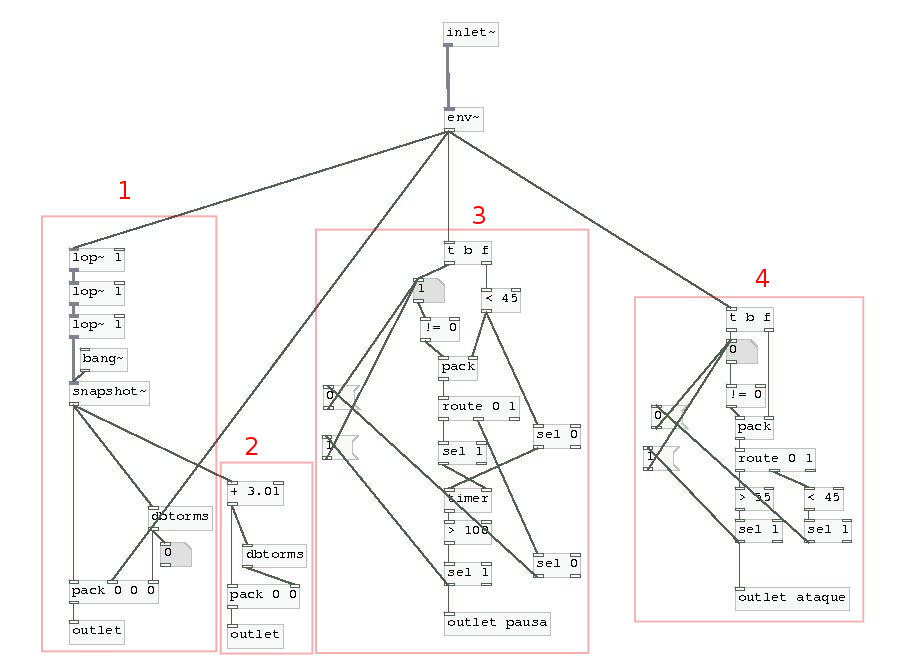
\includegraphics[scale=.5]{sinc-audioanalise-detecta}
\caption{sub-patch que detecta silêncio no áudio de entrada}
\label{[sinc-audioanalise-detecta]}
\end{figure}




Na área 6 vemos um subpatch responsável por detectar
silêncio. Na figura \ref{[sinc-audioanalise-detecta]}


Nesse sub-patch vemos 4 sub-áreas. Nessa implementação
está sendo usada apenas a terceira saída que é a saída do
módulo de detecção de silêncio. O módulo da sub-área 3
basicamente compara as amplitudes que recebe com relação ao tempo.
Nesse algoritmo, se a amplitude de entrada for menor que 45 dB durante
mais de 100 milisegundos um silêncio é detectado.

\subsubsection{Contorno Melódico}
\label{contornos}


As operações com contornos são uma ferramenta poderosa para
composição musical\cite{sampaio08:torno}. A manipulação de contornos
pode ser aplicada a qualquer parâmetro musical.
No Pd, qualquer dado pode facilmente escrito e lido em arrays gráficos.
Ainda com a possibilidade de se desenhar no array com o mouse, podemos
dizer que programar/compôr no Pd cria uma
forte sinestesia visual - sonora, semelhante a escrita
com notação musical tradicional.

Segundo Silva \begin{quote}
               O estudo de contornos é importante porque, assim como conjuntos de notas e motivos,
               contornos podem ajudar a dar coerência a uma obra musical. Eles representam estruturas
		musicais manipuláveis através de várias operações como inversão e retrogradação, e podem
		ser abordados tanto do ponto de vista da análise quanto da composição.
              \end{quote} \cite{sampaio08:torno}.


Iremos mostrar algumas maneiras como observar, guardar e comparar contornos de modo
que possam ser úteis na construção de um diálogo interativo.

Dentro dessa pesquisa, as operações com contornos servem à análise do material musical,
de onde podemos extrair informações da performance. E também como geradores de material
musical, aplicando operações diversas, como veremos na seção \ref{varia-contorno}.
A primeira operação para análise de contornos é a redução para a forma normal. Segundo Silva:

\begin{quote}
 A forma normal de um contorno ocorre quando seus elementos aparecem em ordem
temporal de ocorrência, e com valores definidos de 0 (menor valor) a n − 1 (maior valor),
onde n  representa o número de elementos do contorno . A operação de translação aplicada a um
contorno retorna a sua forma normal (Marvin e Laprade 1987, p. 228). Esta operação
consiste em redefinir o elemento de menor valor para 0, o segundo elemento de menor
valor para 1, o terceiro para 2, e assim por diante. Por exemplo, o contorno P(5 9 6 8)
tem forma normal F(0 3 1 2), pois P0 , elemento de menor valor, é redefinido para 0, P2 ,
segundo elemento de menor valor, para 1, P3 , terceiro de menor valor, para 2, e P1 para
3.
\end{quote}

%% figura midi -> array -> salvando 

\begin{figure}
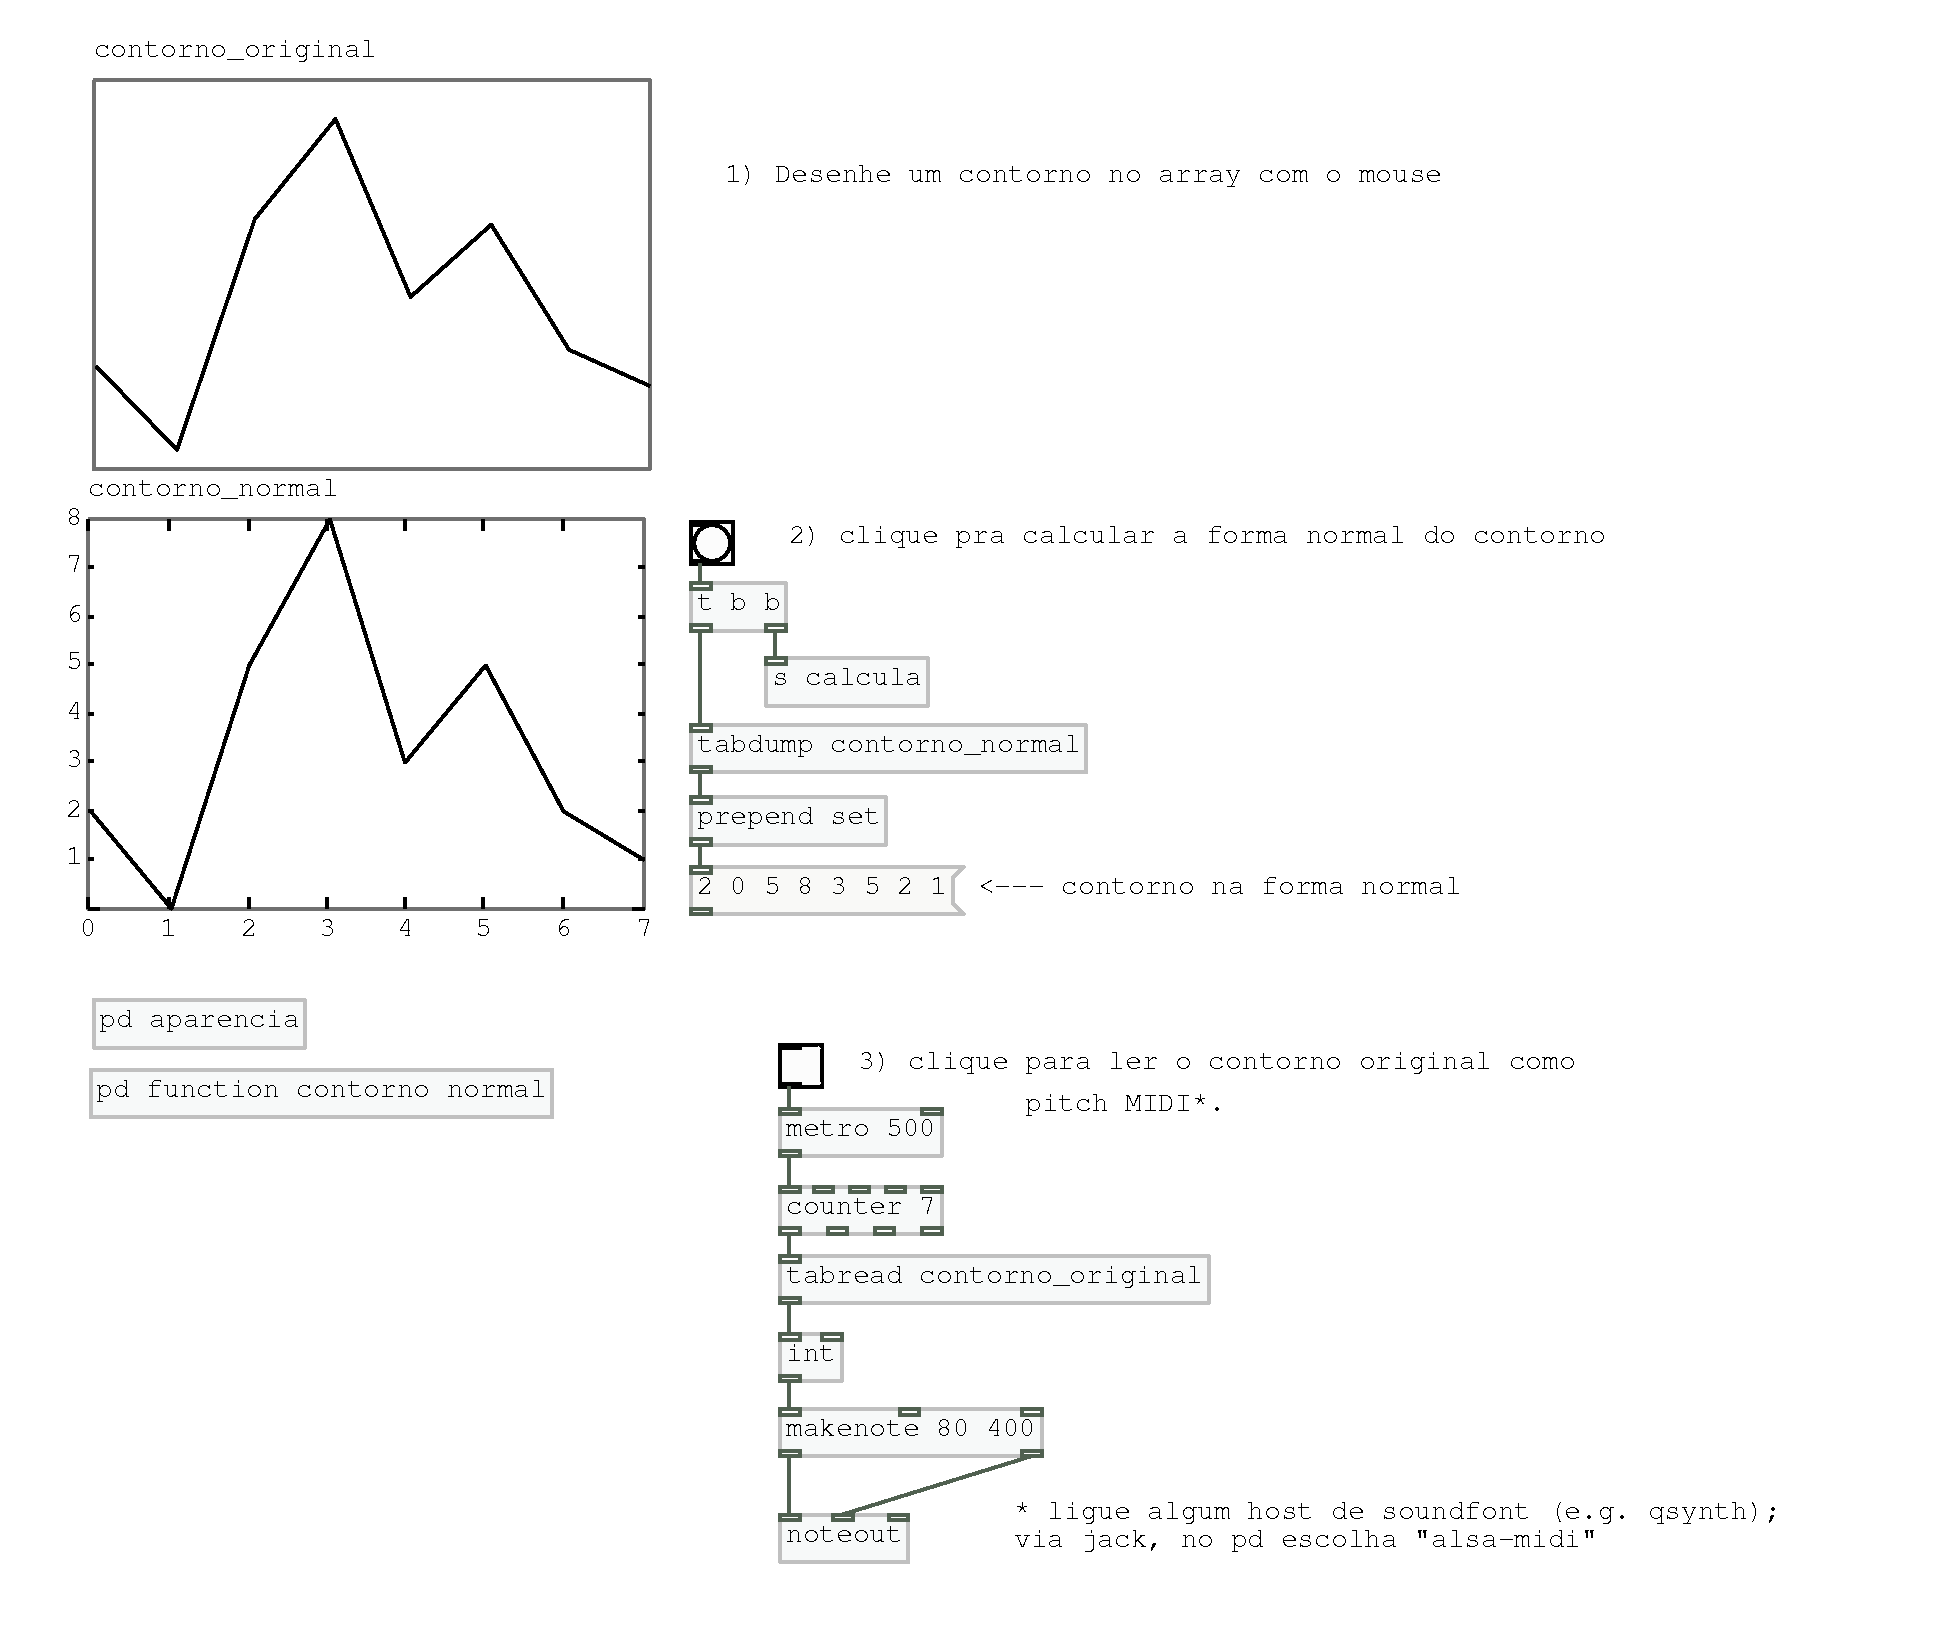
\includegraphics[scale=.2]{contorno-normal}
\caption{Patch mostrando um contorno e sua forma normal}
\label{contorno-normal}
\end{figure}


No Pd, podemos ver um patch que faz a redução do contorno à forma prima 
na figura \ref{contorno-normal}. Nesse patch, o array ``contorno\_original'',
tem oito elementos, variando de 0 a 127 podendo ser alimentado pelo valor de pitch de um fluxo
MIDI. A forma normal é calculada dentro do sub-patch [pd function contorno normal], e após
o cálculo o resultado é escrito no array abaixo ``contorno\_normal''.

\begin{figure}
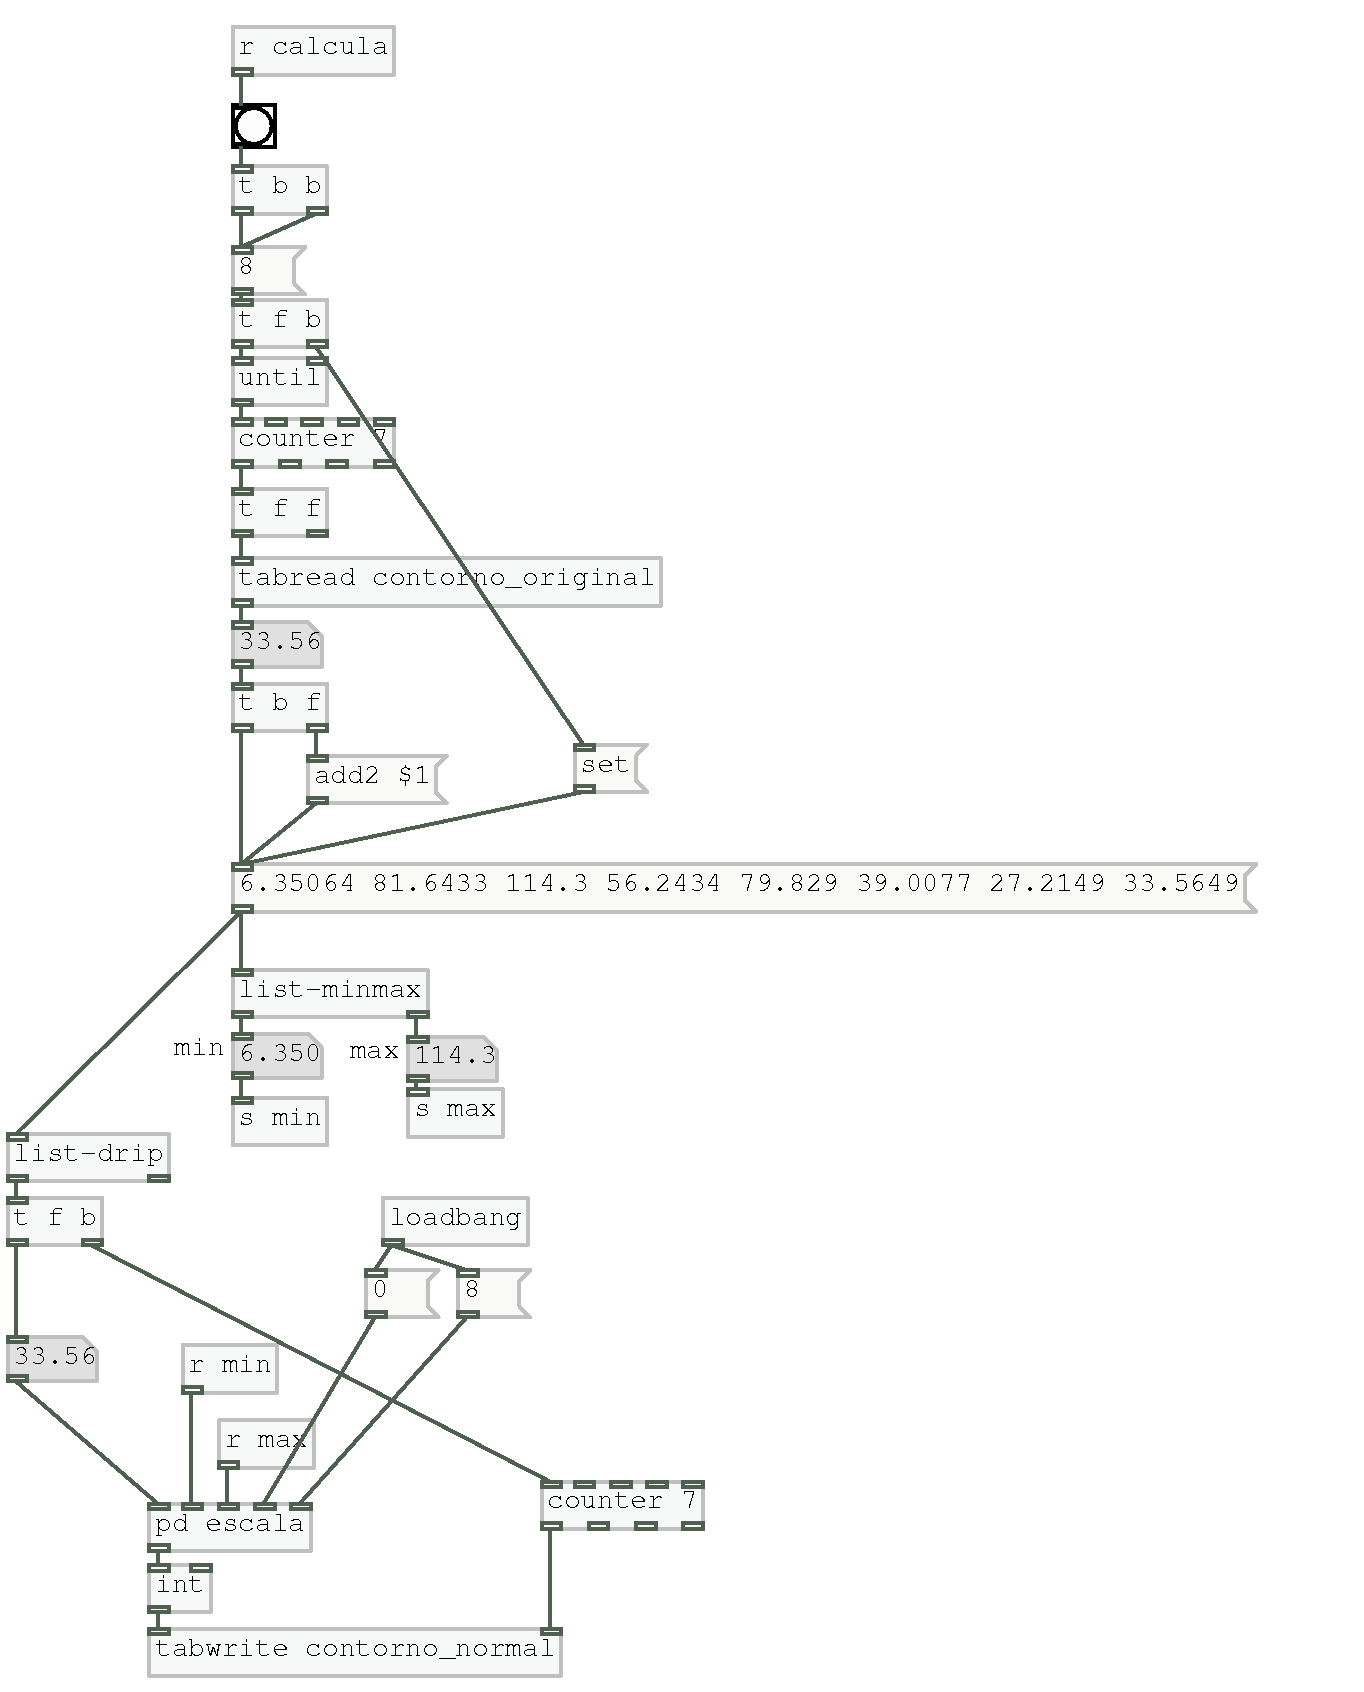
\includegraphics[scale=.6]{func-contorno-normal}
\caption{Operação de redução de um contorno à sua forma normal}
\label{func-contorno-normal}
\end{figure}

Na figura \ref{func-contorno-normal} vemos a operação de redução à forma normal.
Onde primeiro é feito uma leitura do array original com [until] e [tabread]. Após
a leitura é calculado o valor mínimo e máximo com o objeto [list-minmax] e os dois
valores são enviados com as variáveis globais [s min] e [s max].

O mapeamento dos valores é feito de forma linear, usando o patch mostrado na figura \ref{sinc-escala-linear}.
Nesse caso, o menor valor irá equivaler a zero e o maior valor equivaler a oito, que é o
número de elementos do array. Ao final ainda os valores são convertidos para valores inteiros,
antes de serem escritos no array de resultado.

A análise da similaridade entre contornos é uma ferramenta importante dentro
 de um sistema de composição interativa, pois pode revelar emergência e dissolução de 
padrões de execução e improvisação. 
Existe uma crescente bibliografia sobre análise de similaridade de contornos,
como no artigo ``Testing models of Melodic Contour Similarity'' \cite{schmuckler}, onde o autor expõe e compara diversos modelos de análise,
tanto baseados em teoria musical, quanto em modelos abstraídos de experiências
em cognição musical.

\begin{figure}
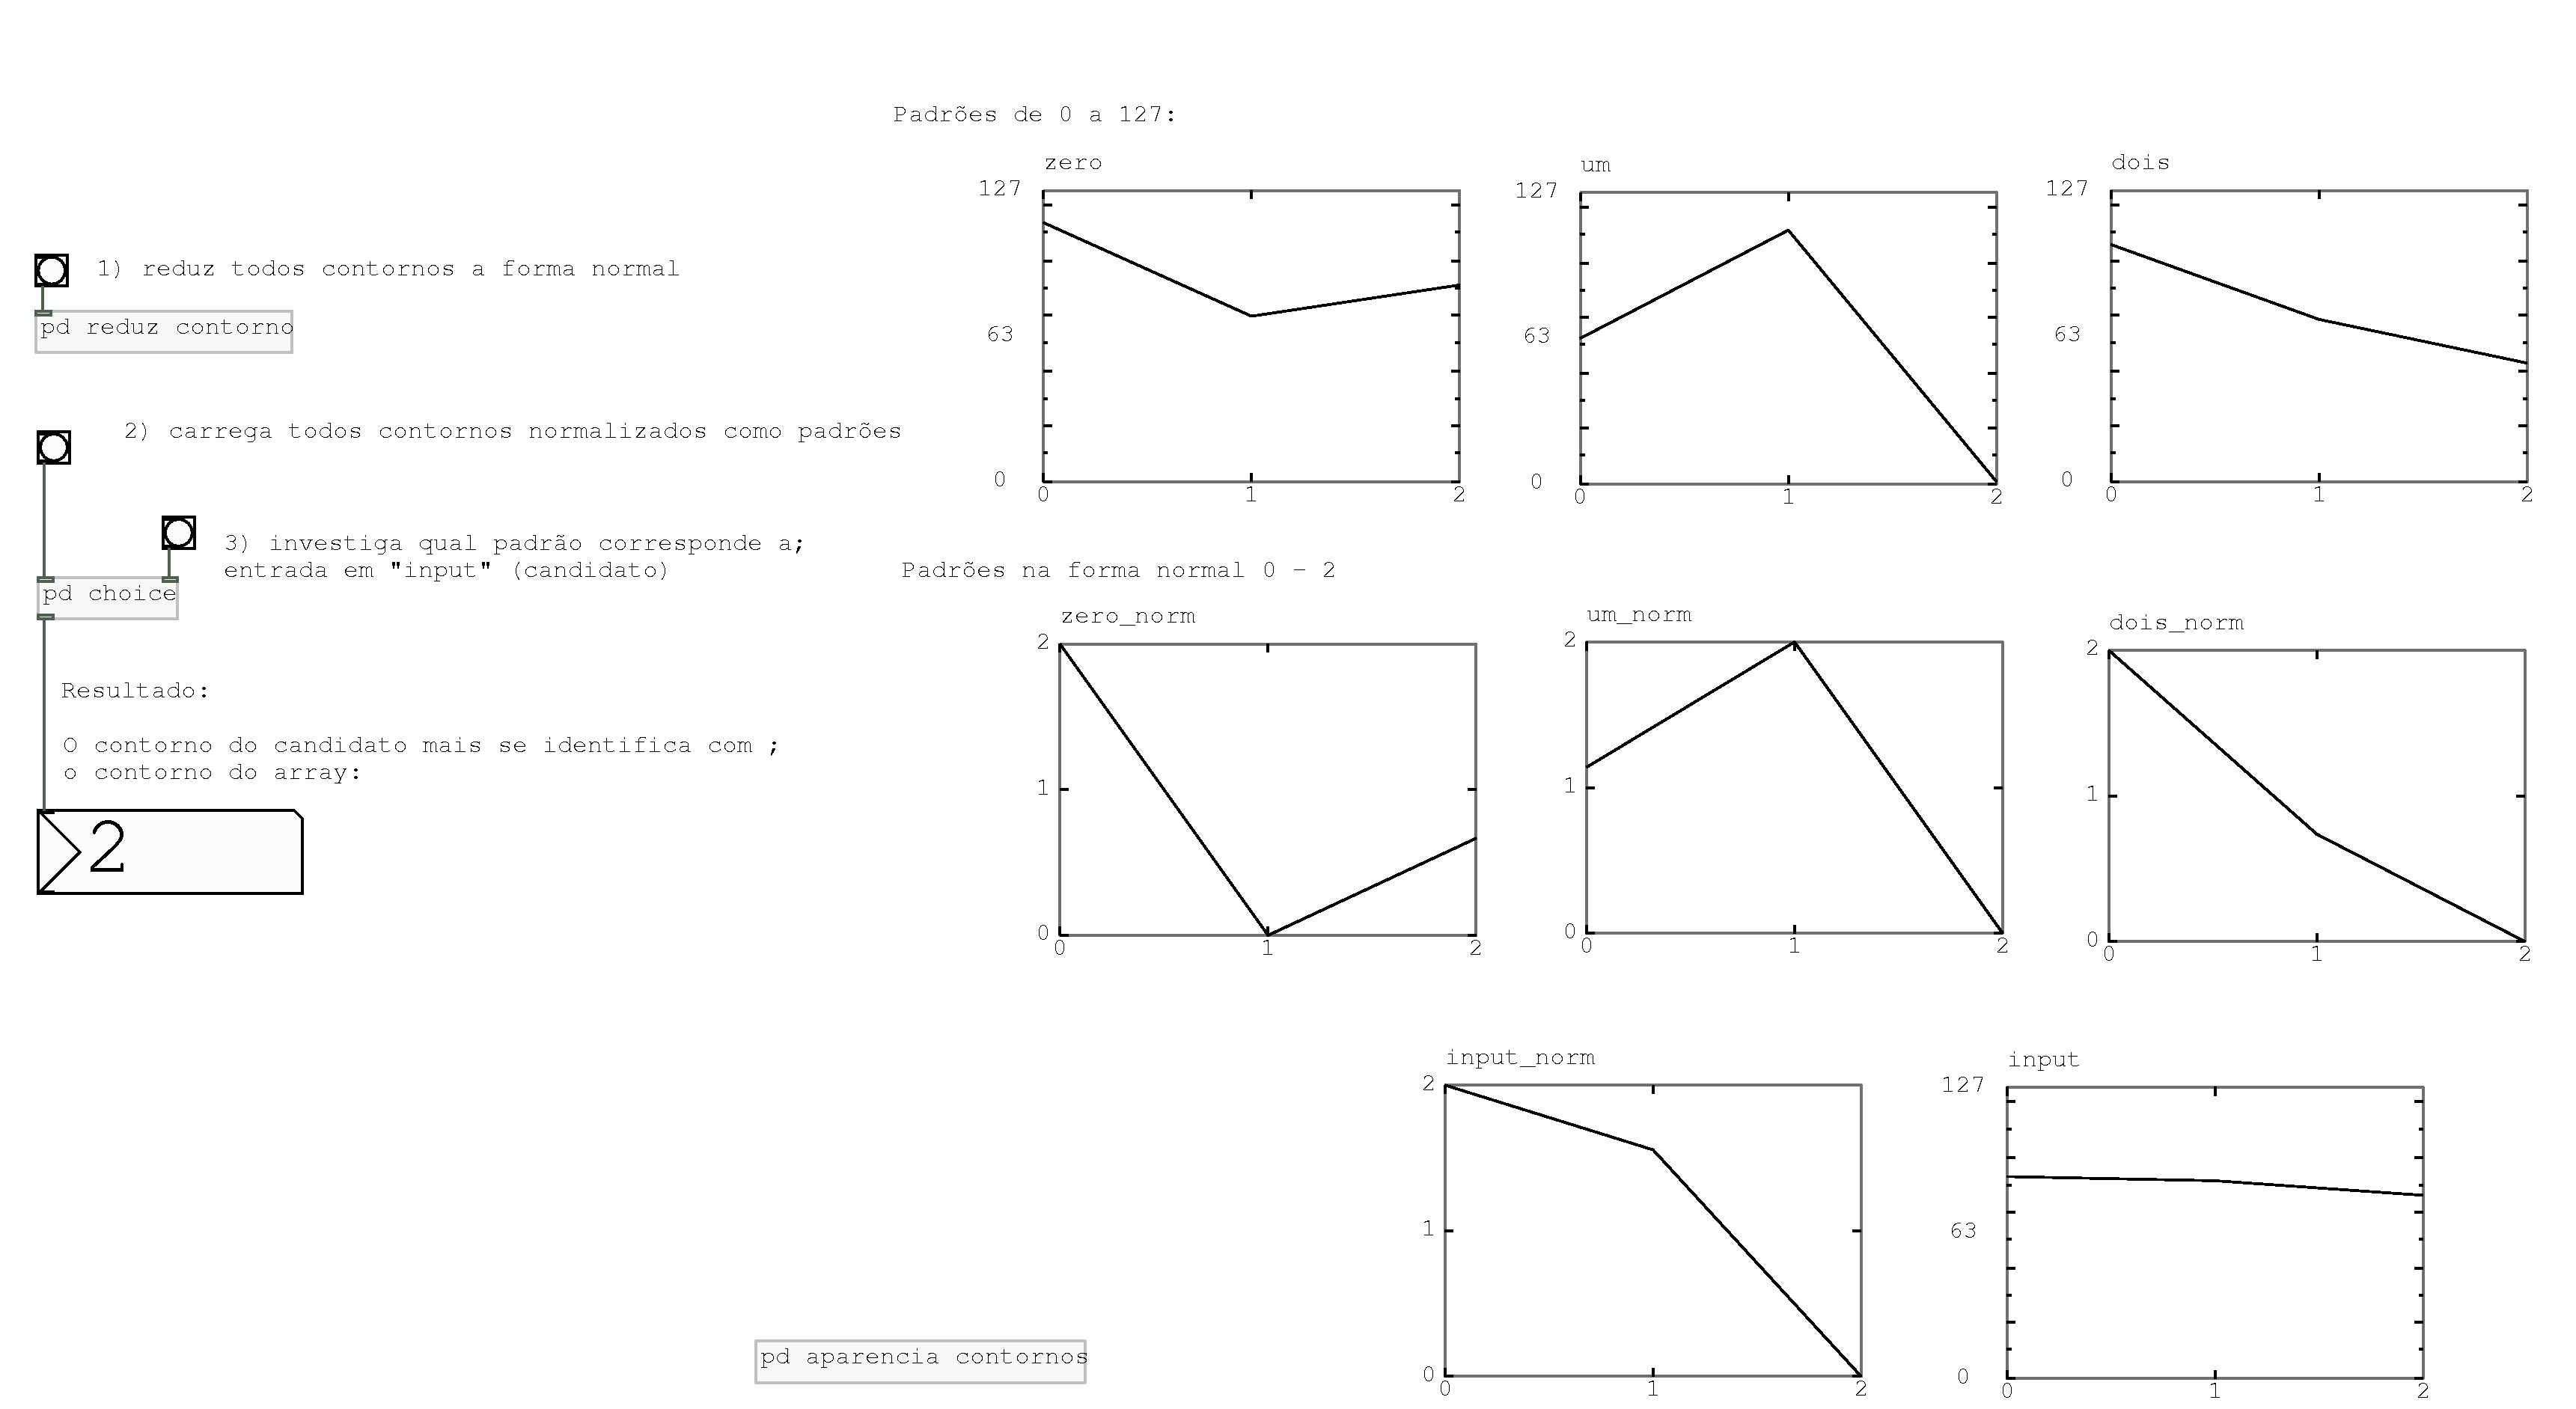
\includegraphics[scale=.4]{similaridade-interface}
\caption{Experimento de análise de similaridade de contornos baseado em banco com 3 modelos}
\label{similaridade-interface}
\end{figure}

A devida análise de similaridade de um contorno melódico deve levar em conta todos
aspectos envolvidos como o timbre, relações de duração e intensidade de cada ponto do contorno.
Apesar da estimativa de similaridade de contornos ser um objeto de pesquisa vasto e complexo, 
consideramos que abordagens
mais simples podem ser úteis no desenho de um sistema de composição interativa.
Apresentamos aqui um primeiro experimento de análise de similaridade, aplicado em
contornos de apenas três elementos. A idéia é que alimentar um banco com três contornos estocados e a cada
novo contorno que chega, o sistema devolve o índice do contorno estocado mais similar.
A interface do experimento pode ser vista na figura \ref{similaridade-interface}.
A primeira etapa do experimento é a redução de todos contornos à forma normal.

\begin{figure}
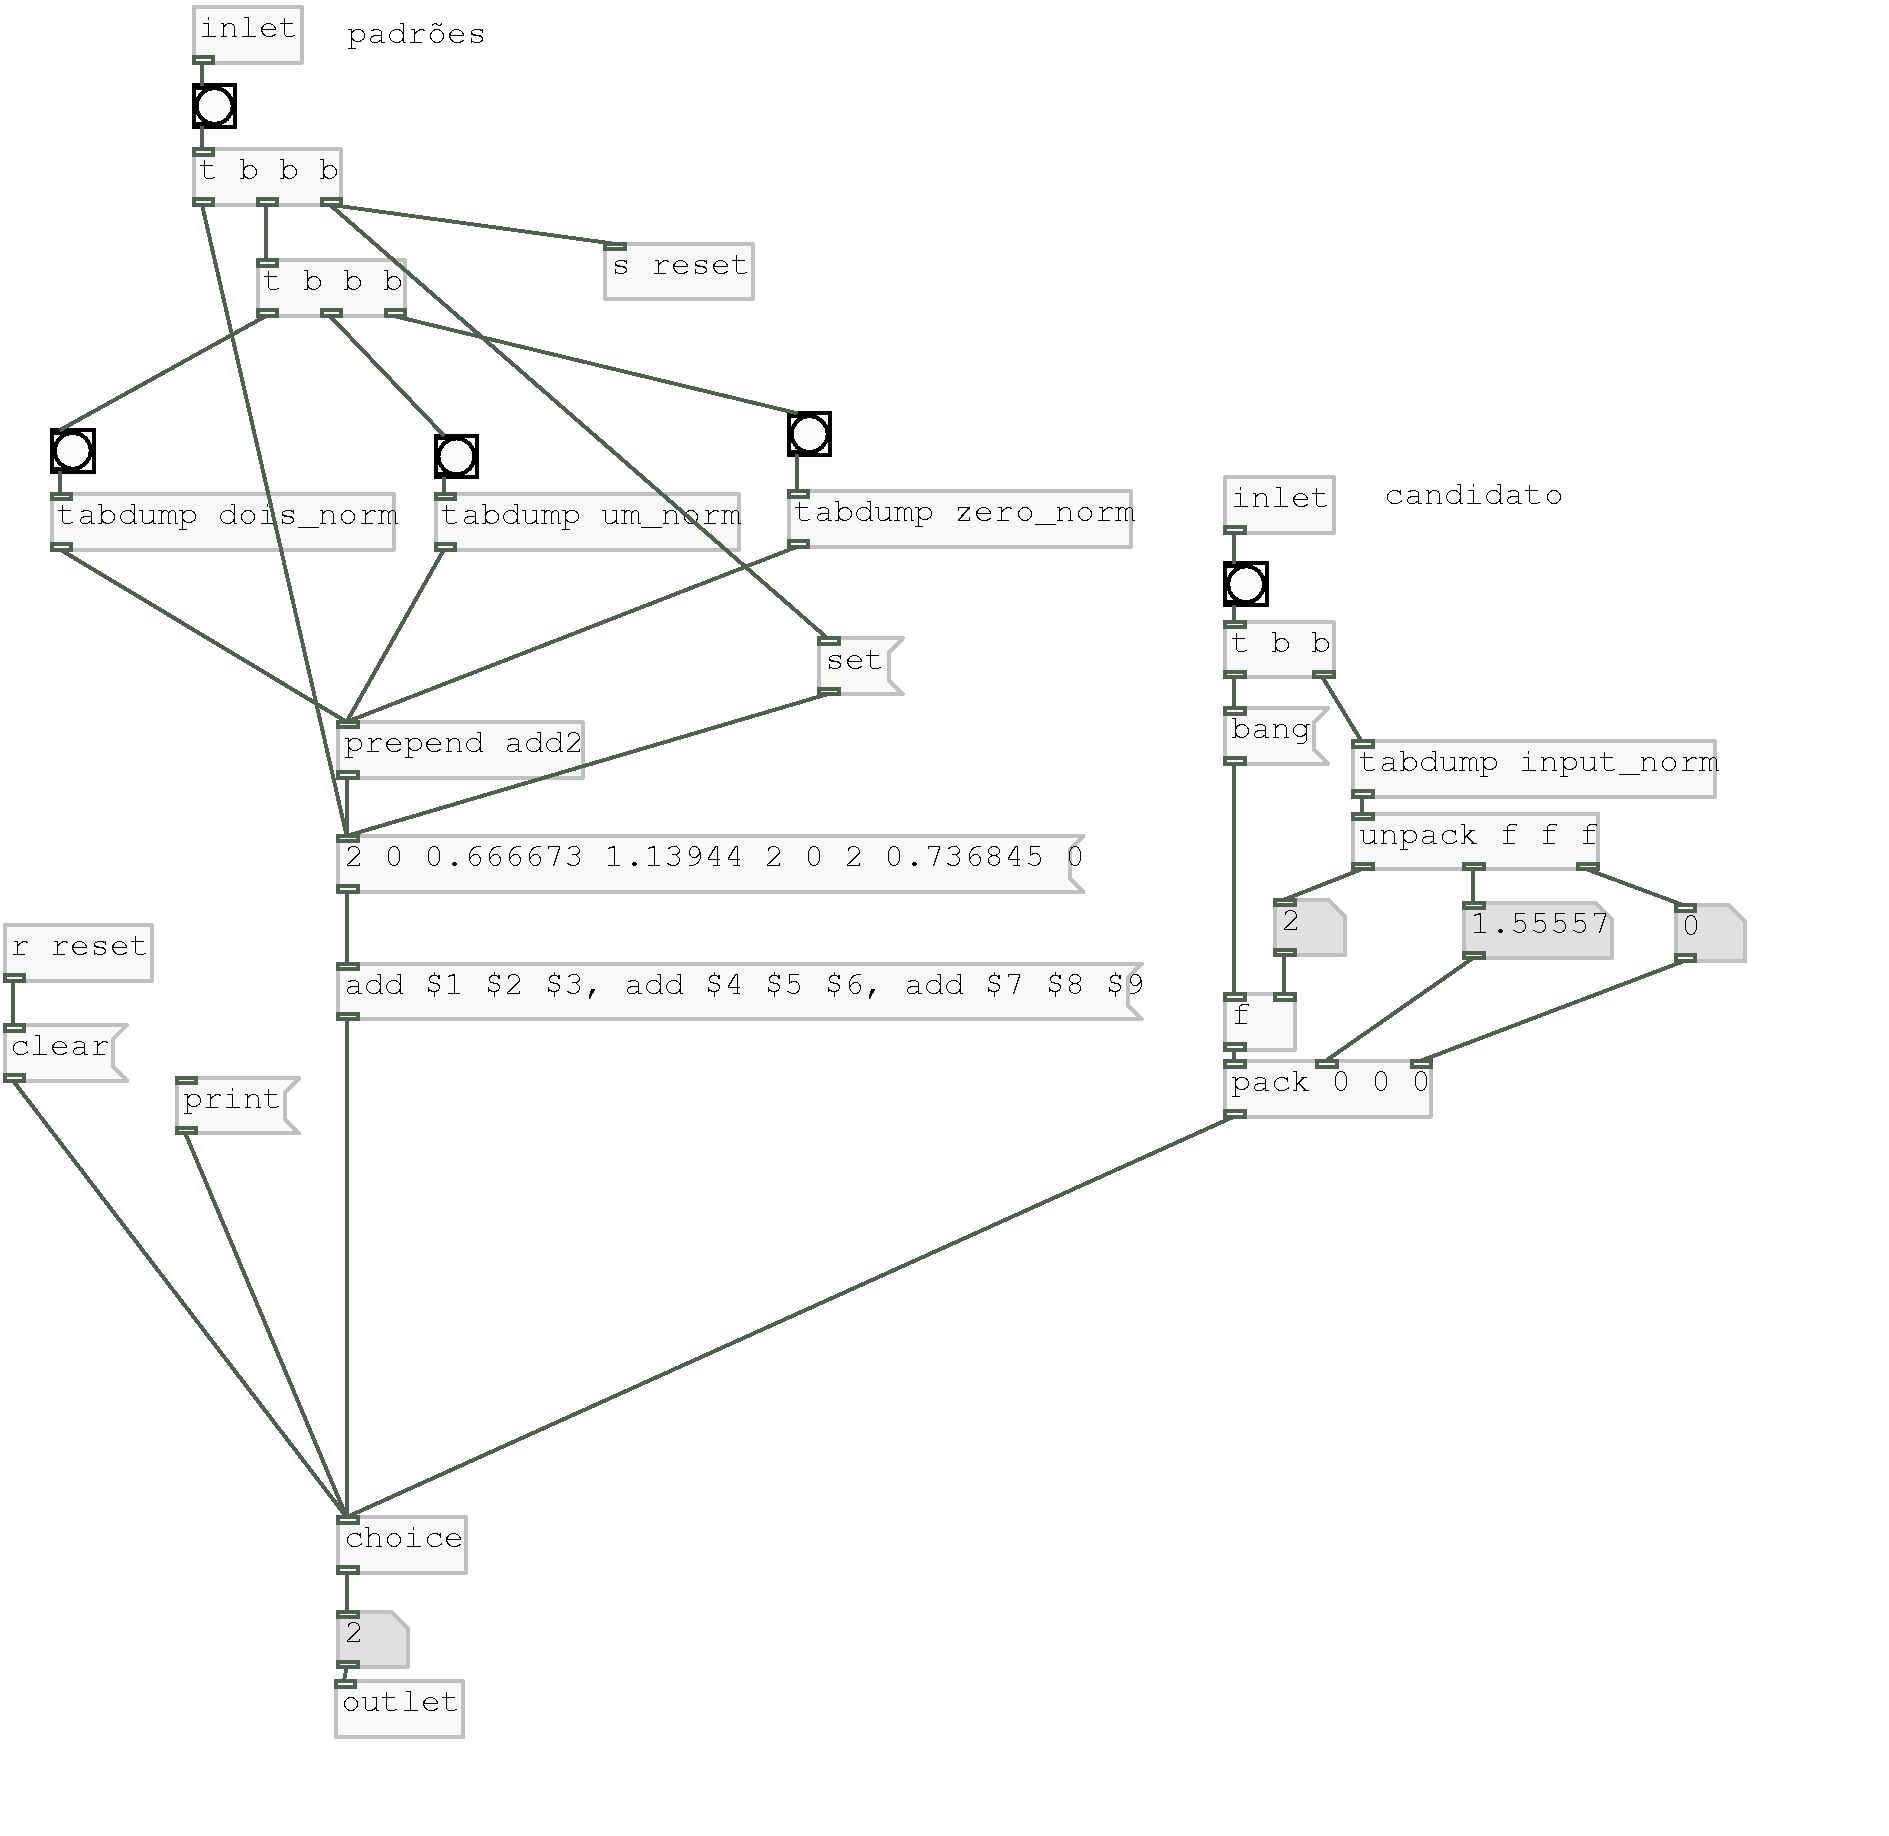
\includegraphics[scale=.5]{similaridade-algo}
\caption{Patch que calcula o índice de similaridade entre contornos}
\label{similaridade-algo}
\end{figure}


Na figura \ref{similaridade-algo} vemos o interior do sub-patch [pd choice].
Onde os três contornos na forma normal são enviados ao objeto [choice], cada um
precedido da mensagem ``add''. A cada lista que chega em [choice], o objeto retorna
o valor da lista estocada que mais se aproxima.

O objeto [choice] estoca uma lista de vetores, cada um podendo ter até dez
elementos. Quando mandamos uma nova lista de números, é retornado o índice
do vetor conhecido que se combina mais proximamente com a nova lista. A qualidade
da combinação  é o produto interno dos dois vetores após outra normalização
interna. O vetor que tem a direção mais próxima da lista/vetor de entrada ganha e seu
índice é enviado para a saída. Esse objeto pode ser usado em diversas outras situações
de análise em tempo-real e sua interface simples possibilita uma rápida prototipação.

Um aprofundamento da pesquisa em contornos necessita uma implementação de identificação
mais completa, como uma implementação de redes neurais artificiais por exemplo. Além
de revisão e teste dos modelos analíticos citados na bibliografia da área.
Nessa pesquisa, a próxima etapa será a integração da análise de contorno com os
mecanismos de geração de material musical.

\subsubsection{Permeabilidade melódica}

\begin{figure}
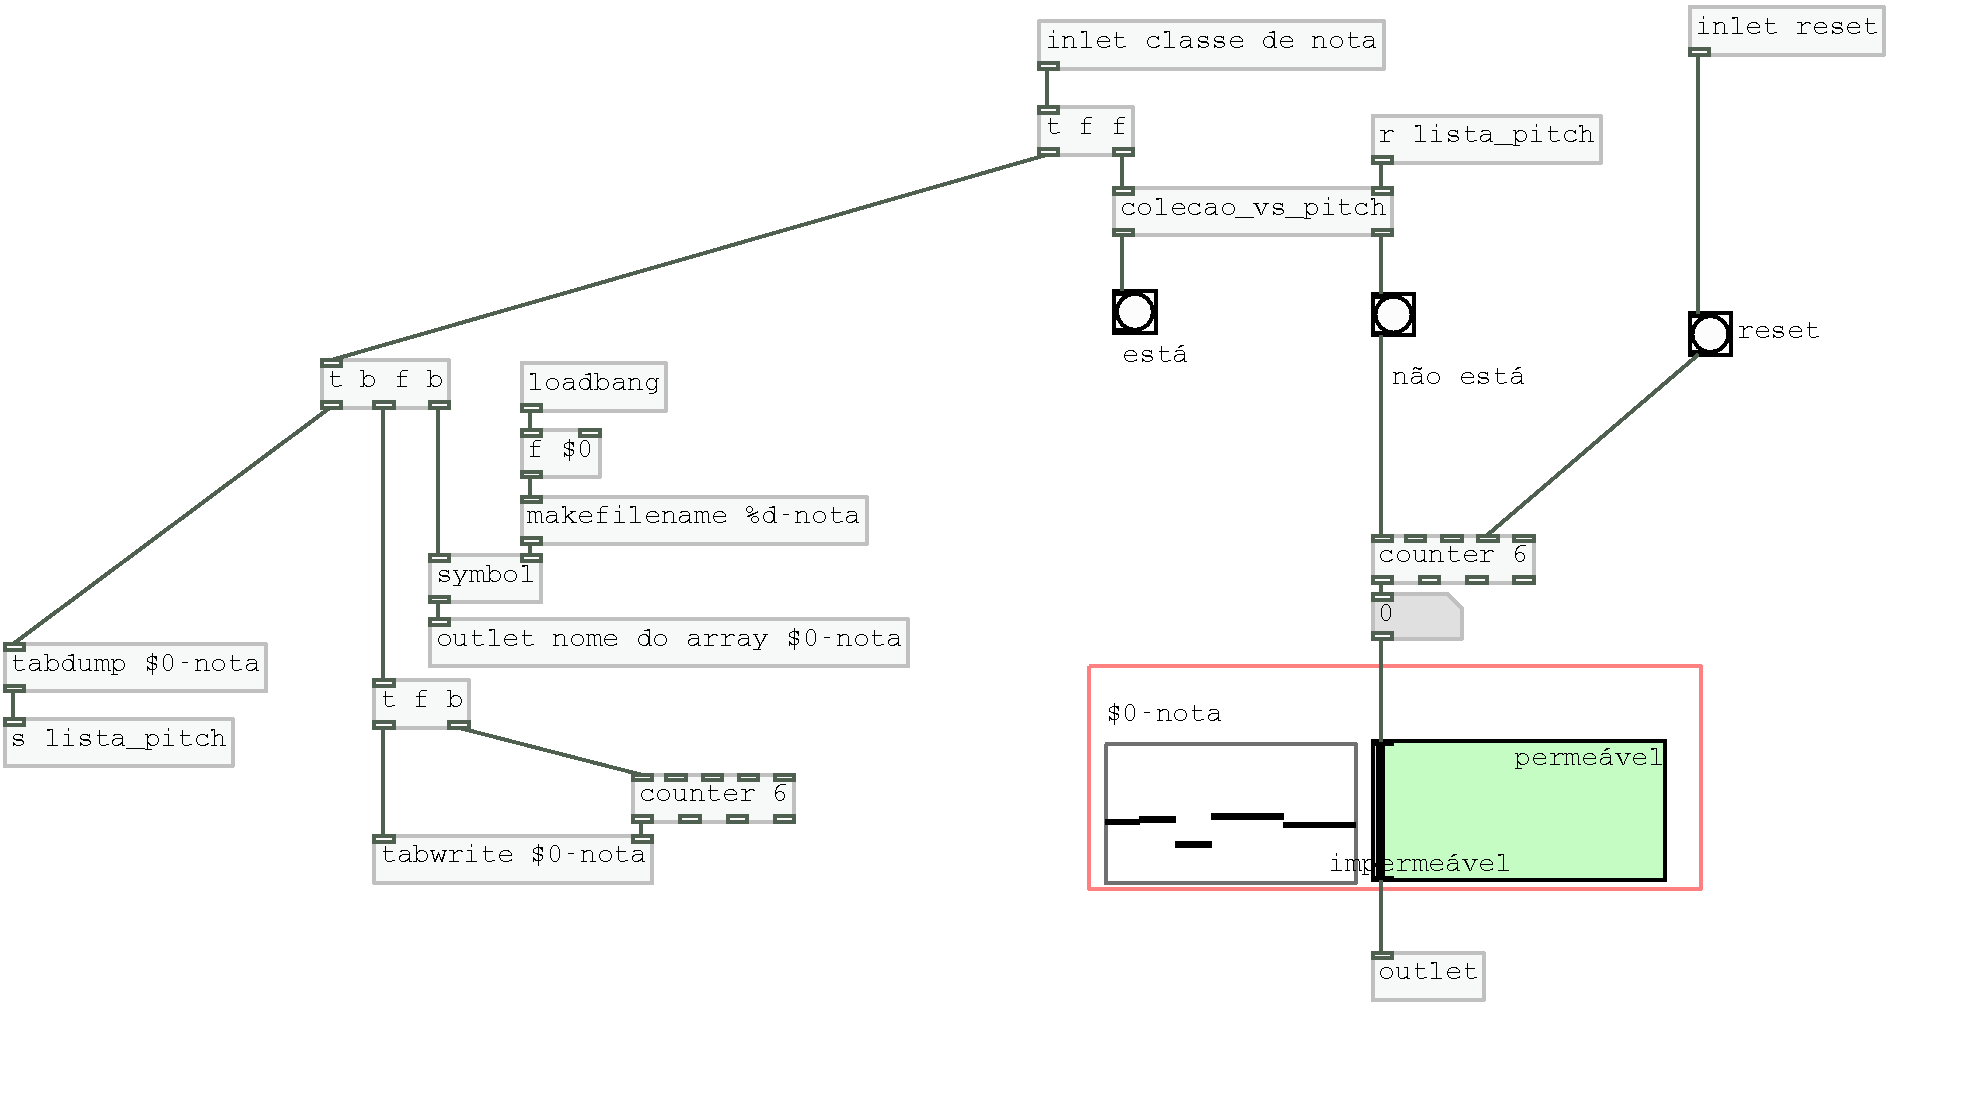
\includegraphics[scale=.5]{permeabilidade}
\caption{Patch que calcula o índice de permeabilidade melódica em fluxo melódico}
\label{permeabilidade}
\end{figure}

\begin{figure}
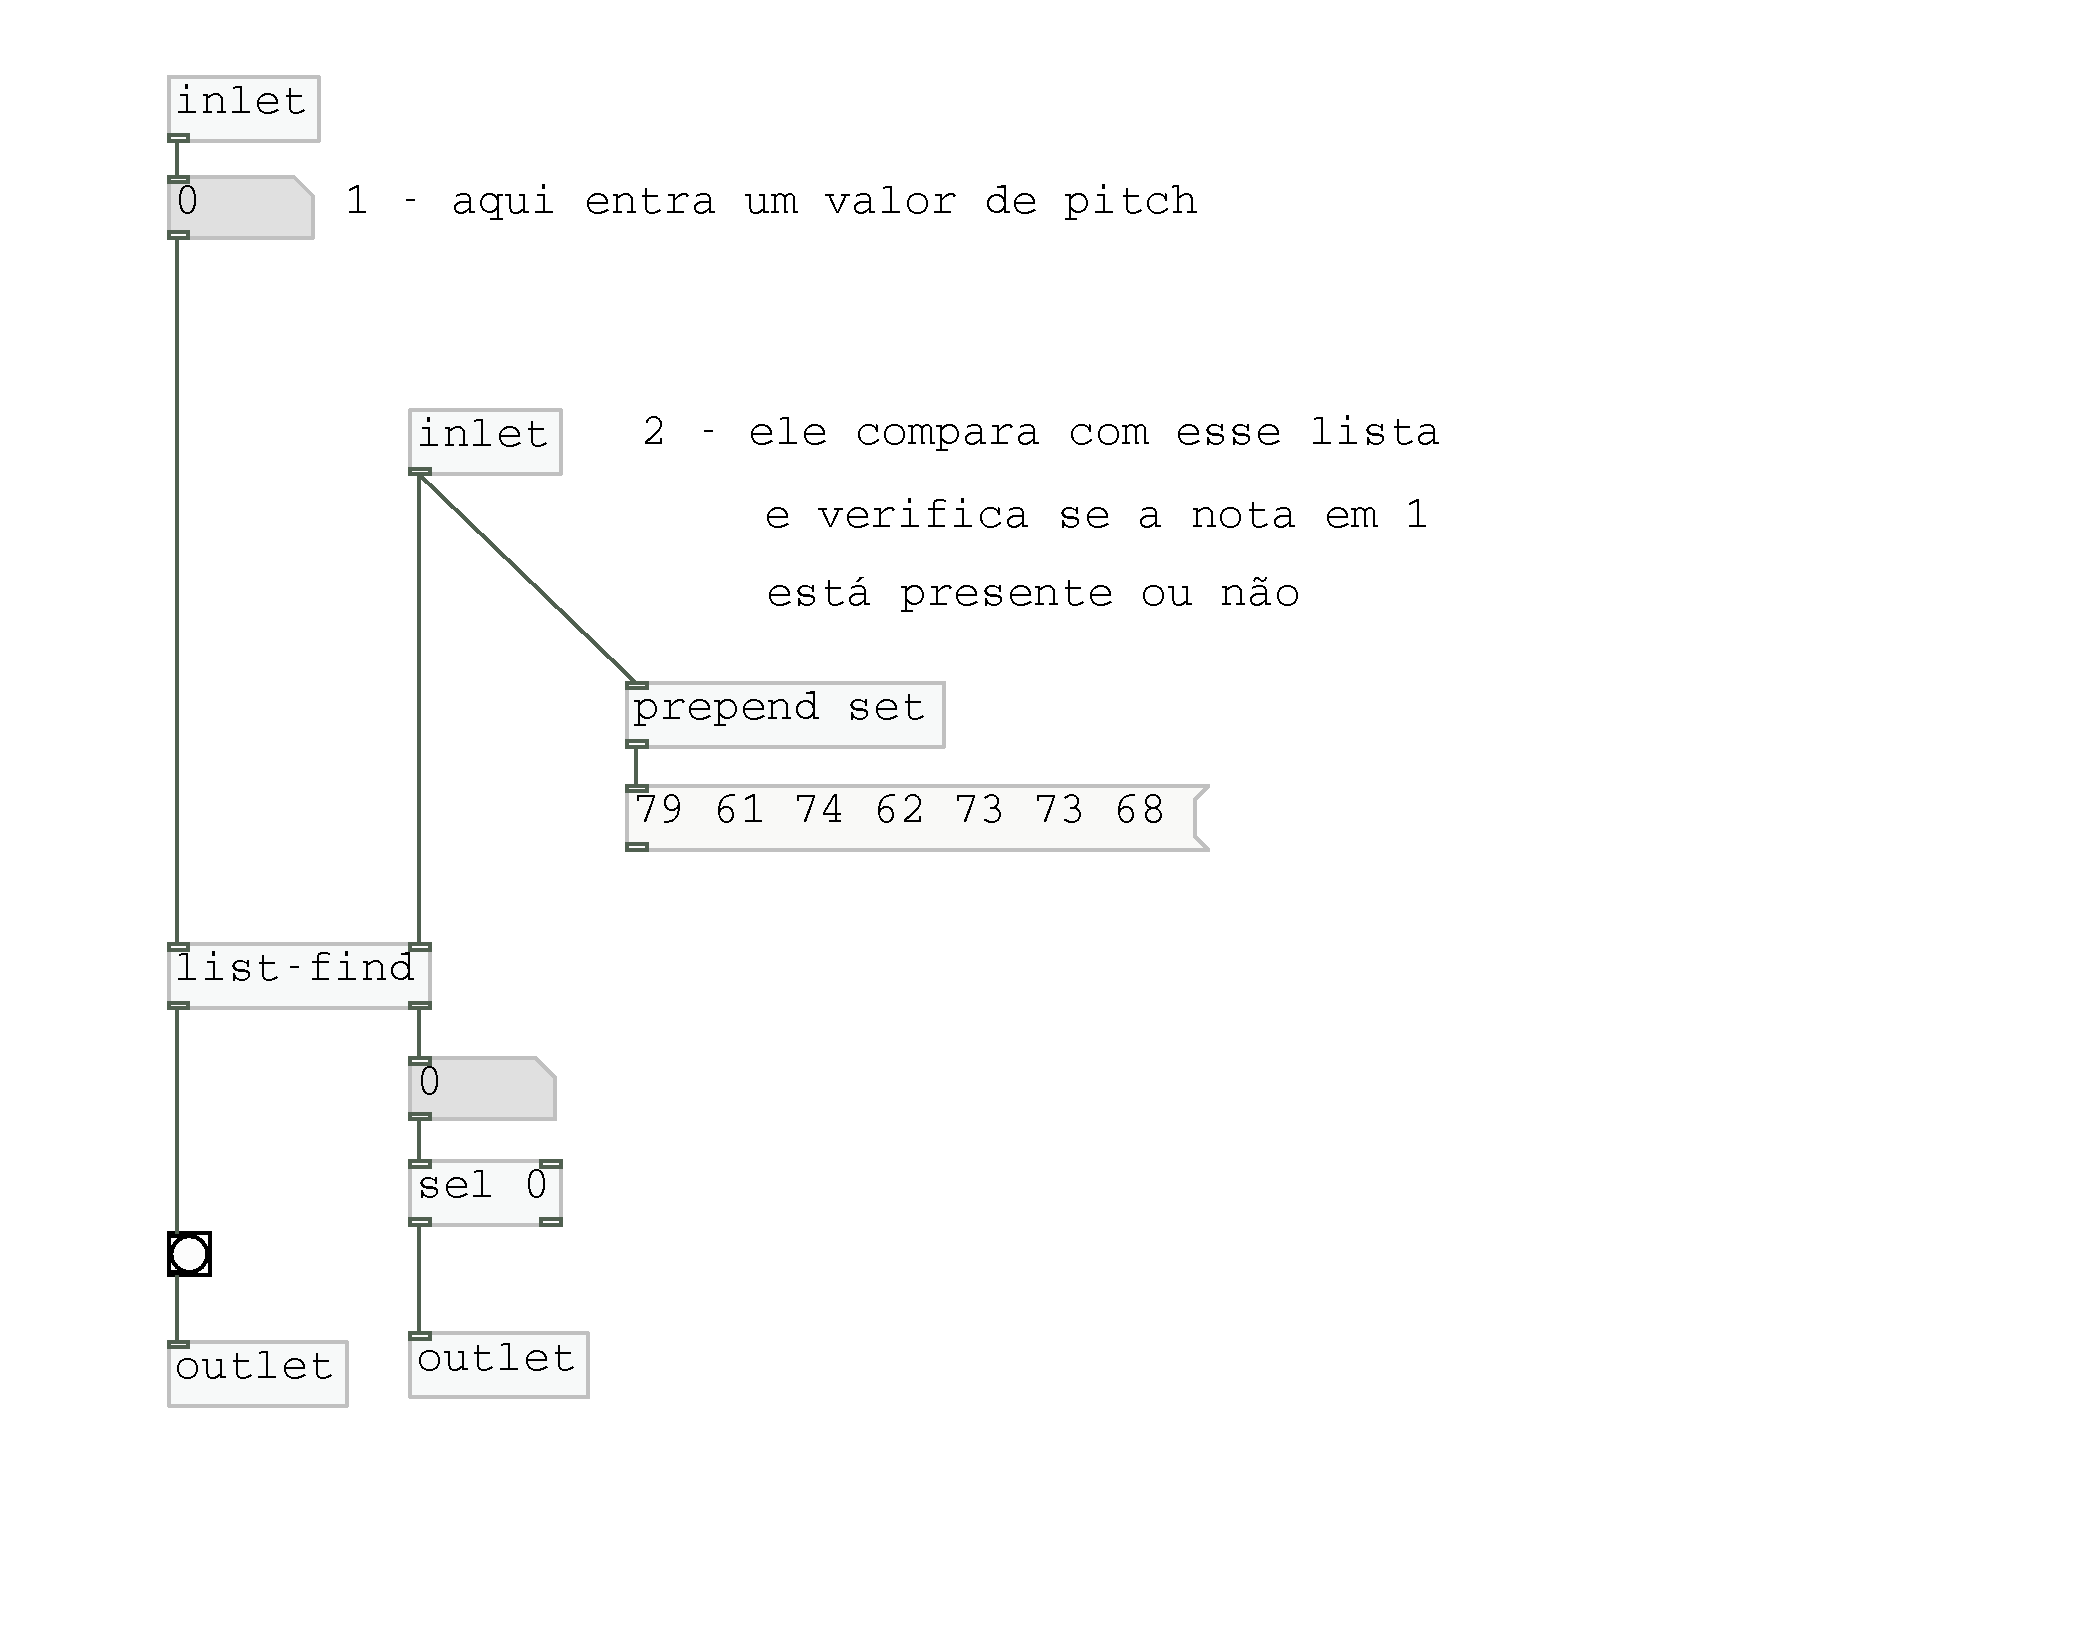
\includegraphics[scale=.5]{colecao_pitch}
\caption{Patch que ananlisa a ocorrência de uma classe de nota em uma lista de classes de notas}
\label{colecao-pitch}
\end{figure}



Uma das características de um sistema interativo é a capacidade do sistema
de emular técnicas composicionais e responder ``compondo'' em tempo-real a
estímulos musicais provindos de músicos humanos. Para isso deve-se implementar
no sistema técnicas de composição que sejam a maneira como o sistema ``percebe''
e responde aos estímulos. Nesse sentido o conceito de “permeabilidade” de 
alturas \cite{ligeti58:transformacoes} pode ser um conceito muito útil se aplicado aos parâmetros
de análise das alturas pelo sistema. 

\begin{quote}
  A tendência geral conduz, então, para a insensibilização da
  fisionomia dos intervalos. Sucessões de tons e superposições
  verticais tornam-se, em grande escala, indiferentes frente aos
  intervalos dos quais provem; conceitos como consonância e
  dissonância se tornam irrelevantes: tensões e distensões podem ser
  obtidas com qualidades estatísticas da forma, como relação de
  registros, densidade ou tipos de tecido das estruturas [...] A perda
  da sensibilidade perante os intervalos conduz a um estado que
  poderíamos chamar de permeabilidade. Isso significa que estruturas
  de diferentes qualidades que transcorrem simultaneamente podem
  interpenetrar-se e mesmo dissolver-se completamente mudando apenas
  as relações de densidade horizontal e vertical, sendo indiferente,
  em princípio, quais intervalos se cruzam em detalhe [...] Embora a
  permeabilidade não tenha tido, até o momento, nenhuma influência
  decisiva sobre a forma, não era desconhecida nos estilos musicais
  antigos. Quem teve o grau mais baixo de permeabilidade até agora
  talvez tenha sido Palestrina, em cuja música vozes simultâneas,
  reguladas por leis expressas univocamente, enrolavam-se umas na
  outras. As possibilidades de combinações intervalares, fortemente
  fixadas, não permitiam a menor ambigüidade no transcurso das
  estruturas; portanto, as relações entre dissonância e consonância
  estavam tratadas, naquele estilo, com o maior cuidado. \cite{ligeti58:transformacoes}
\end{quote}
 
Ligeti fala aqui sobre uma permeabilidade dos intervalos de altura,
pode-se pensar em ampliar, e implementar no sistema, esse pensamento
de permeabilidade para conceitos como permissividade evolutiva,como por
exemplo, a permissividade de emergência de estruturas derivadas do material 
da própria análise do timbre do áudio de entrada. Outro exemplo poderia ser a 
emergência de certos comportamentos contrastantes em trechos isolados do material.
A permeabilidade de alturas pode ser um parâmetro de análise das alturas 
de uma performance em tempo-real. Outra possibilidade de aplicação pode ser o
controle geral da permeabilidade de alturas, tendo o sistema a capacidade de
classificar a porcentagem da permeabilidade envolvida em cada trecho. 

\begin{quote}
  A insensibilidade frente aos intervalos e a grande permeabilidade é
  ainda mais importante na música de Cage e seu círculo, proveniente
  de princípios totalmente diferentes. Existem obras de Cage que podem
  ser executadas tanto isoladamente quanto de forma simultânea com
  outras partituras onde, então, cada peça se transforma em capa de
  uma possível superposição que, se bem será mais densa que suas
  componentes, não está composta de forma diferente delas. A
  indiferença de tais estruturas, resultado de manipulações com o
  acaso, está estreitamente relacionada com a indiferença dos produtos
  automáticos da música serial primitiva. Essa indiferença tende
  também, por sobre as relações intervalares, para uma ampliação das
  outras dimensões musicais. Uma vez eliminadas as relações
  hierárquicas, afrouxadas as pulsações métricas simétricas,
  transposto os graus de duração, de intervalos e de timbre das
  distribuições seriais, torna-se cada vez mais difícil controlar os
  contrastes. \cite{ligeti58:transformacoes}
\end{quote}


O objeto [sinc-permeabilidade] apresenta um primeiro estudo sobre 
o cálculo da permeabilidade melódica aplicada em composição interativa.
A idéia é verificar a presença de um valor de classe de nota em uma lista
de valores dinâmicos. Na figura \ref{permeabilidade} podemos ver um [inlet classe de nota]
que envia o mesmo valor para o array [\$0-nota] e para a abstração [colecao\_vs\_pitch].
O array [\$0-nota] coleciona as últimas seis classes de notas e envia uma lista com
todos os valores através da variável [send lista\_pitch]. Na figura \ref{colecao-pitch}
podemos ver a estrutura da abstração [colecao\_vs\_pitch] que verifica a ocorrência
da atual classe de notas dentro das últimas seis classes passadas. O resultado é enviado
para o contador [counter] e quanto mais notas ``novas'' surgem, maior é o índice de 
permeabilidade melódica.


Podemos pensar no conceito de permeabilidade como uma técnica composicional
que pode ser quantificável, portanto passível de ser implementada em um programa
de computador e agregada ao sistema que aqui se propõe. Esse conceito pode ser
aplicável aos outros parâmetros do som e radicalizando esse pensamento podemos
pensar no ato composicional como um controle dinâmico entre diversos níveis de 
permeabilidade em todos parâmetros do som.




\subsection{Análise rítmica}

Se considerarmos que um evento sonoro pode ser descrito por um espaço multidimensional
onde cada parâmetro seria uma dimensão (notas, registros, timbre, etc..), podemos
imaginar o ritmo como uma outra multidimensão paralela e sincronizada com as outras.
O aspecto rítmico de um evento sonoro pode ser descrito por:
\begin{itemize}
 \item relações de durações entre ataques de notas;
\item relações de acento (amplitude) entre ataques de notas;
\item densidade de eventos em recortes de tempo;
\item descrição de índices de estabilidade em diferentes recortes temporais;
\end{itemize}

Todos esses níveis se entrecruzam para formar um cenário que pode explicar mais detalhadamente
os elementos rítmicos de um evento sonoro. O objetivo dessa seção é apresentar o desenvolvimento de
ferramentas para a análise das múltiplas camadas de descrição do ritmo.


% Aqui apresentar exemplos com formas de onda em arrays e mostrando na figura
% onde é mais denso, onde é mais instável e hierarquia de intensidade em trechos.
% 
% Mostrar também trechos maiores com índices de estabilidade.



\subsubsection{Objeto [sinc-calc-ritmo]}

Uma das questões perseguidas é o fato do sistema ter conhecimento do atual nível de 
estabilidade rítmica. Isso pode ser alcançado por uma relação que considere variações
de pulso e alternância e variações de padrões rítmicos de tamanhos diferentes.

\begin{figure}
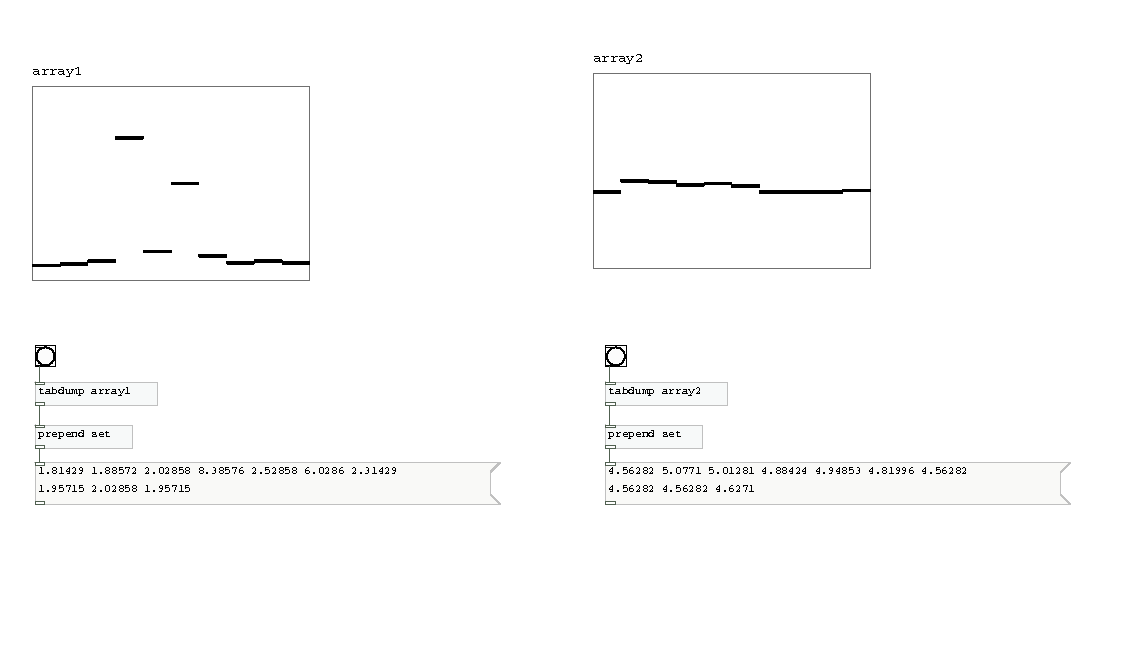
\includegraphics[scale=.6]{prot5a}
\caption{análise de estabilidade rítmica}
\label{prot5a}
\end{figure} 

Na \ref{prot5a} é mostrado dois arrays, idealmente esses arrays representam tabelas
de probabilidades de padrões rítmicos, onde cada elemento no array representa um
padrão diferente e quanto mais alto significa que teve mais ocorrẽncias.
Por exemplo, cada vez que um determinado padrão de 4 valores de duração é tocado, 
o índice na tabela correspondente a aquele padrão é incrementado. O objetivo ideal
é um mecanismo que possa retornar uma resposta do tipo:
``o array1 é mais estável que o array2''. Apenas olhando fica fácil de identificarmos
no array1 que os padrões 3 e 5 tem mais probabilidade de ocorrer pelo seu histórico,
contribuindo assim para uma sensação de estabilidade rítmica. Enquanto que o array2,
tem probabilidades próximas de quase todos padrões criando uma sensação de imprevisibilidade
e fragmentação.


\begin{figure}
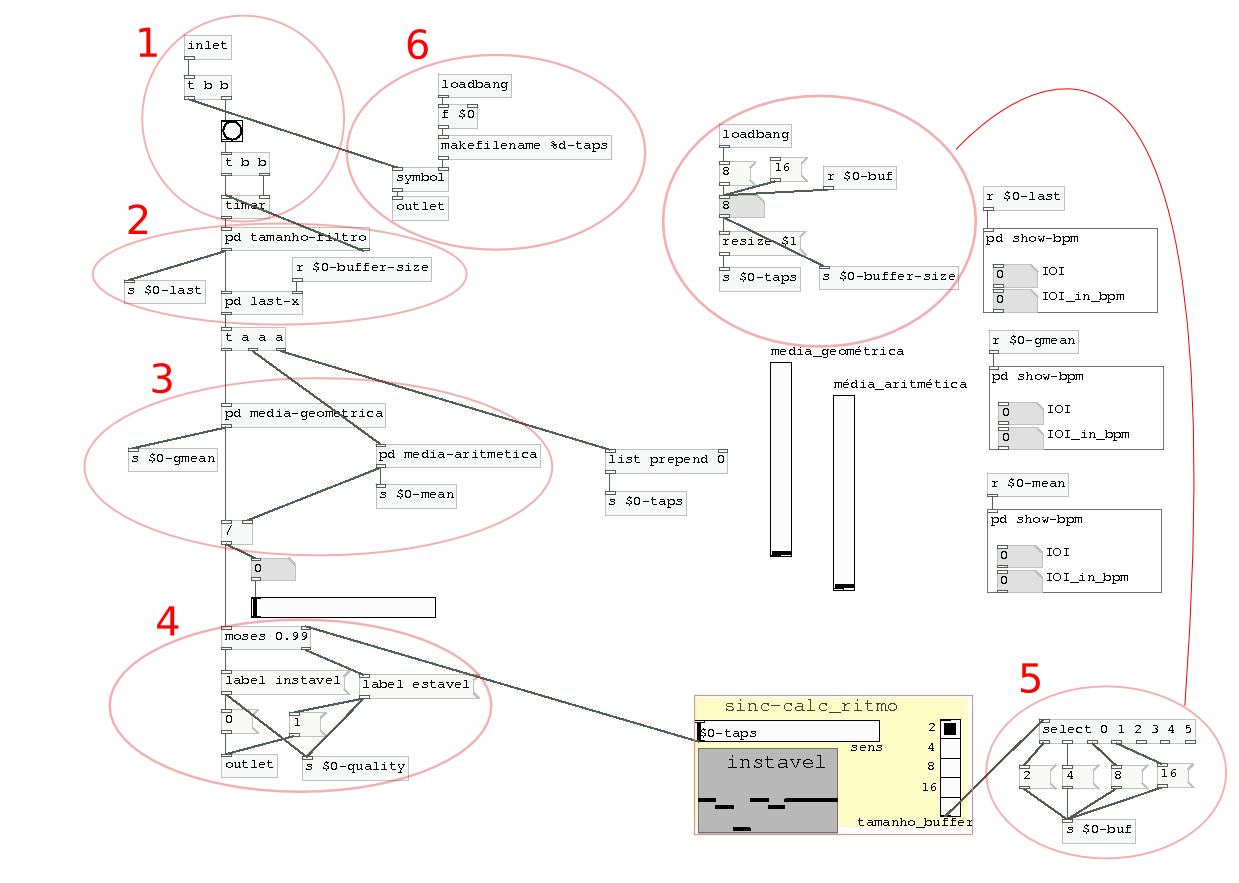
\includegraphics[scale=.5]{sinc-calc-ritmo}
\caption{análise de estabilidade rítmica}
\label{[sinc-calc-ritmo]}
\end{figure}

No patch da \ref{[sinc-calc-ritmo]} é apresentado um método de classificação de estabilidade
de sequência de pulsos. Primeiro são calculadas as distâncias entre cada ataque
sonoro, depois filtrado em [pd filter-range] e colocado em uma tabela dinâmica em
[pd last-x]. 


\begin{figure}
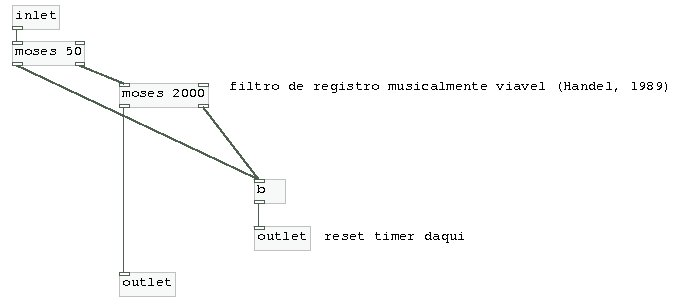
\includegraphics[scale=.6]{sinc-calc-ritmo1}
\caption{filtro de registro de durações}
\label{[sinc-calc-ritmo1]}
\end{figure}

\begin{figure}
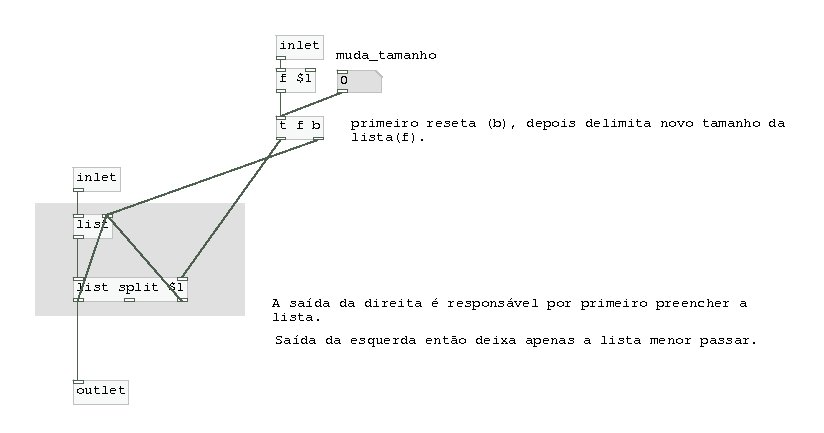
\includegraphics[scale=.6]{sinc-calc-ritmo2}
\caption{lista de durações}
\label{[sinc-calc-ritmo2]}
\end{figure}

Nas figuras \ref{[sinc-calc-ritmo1]} e \ref{[sinc-calc-ritmo2]}, podemos
ver a constituição interna dos sub-patchs [pd filter-range] e [pd last-x].
O tamanho da tabela sempre pode ser redimensionado em tempo-real através
da variável \textit{0-buffer-size} então é calculado ao mesmo tempo a média geométrica
e a média aritmética e os resultados são executados na expressão definida por uma
divisão da média geométrica pela média aritmética. %% isso poderia ser definido em notação matemática :)
Ao resultado dessa divisão é aplicado um filtro com [moses] onde se pode calibrar
a sensibilidade do valor do índice final.




\begin{figure}
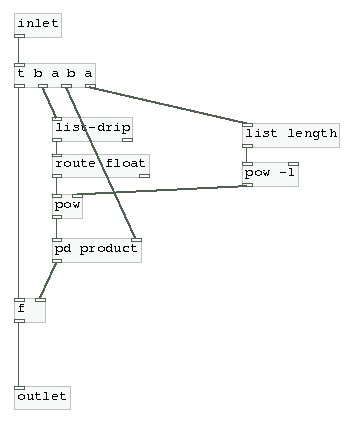
\includegraphics[scale=.6]{sinc-calc-ritmo3}
\caption{média geométrica}
\label{[sinc-calc-ritmo3]}
\end{figure}

\begin{figure}
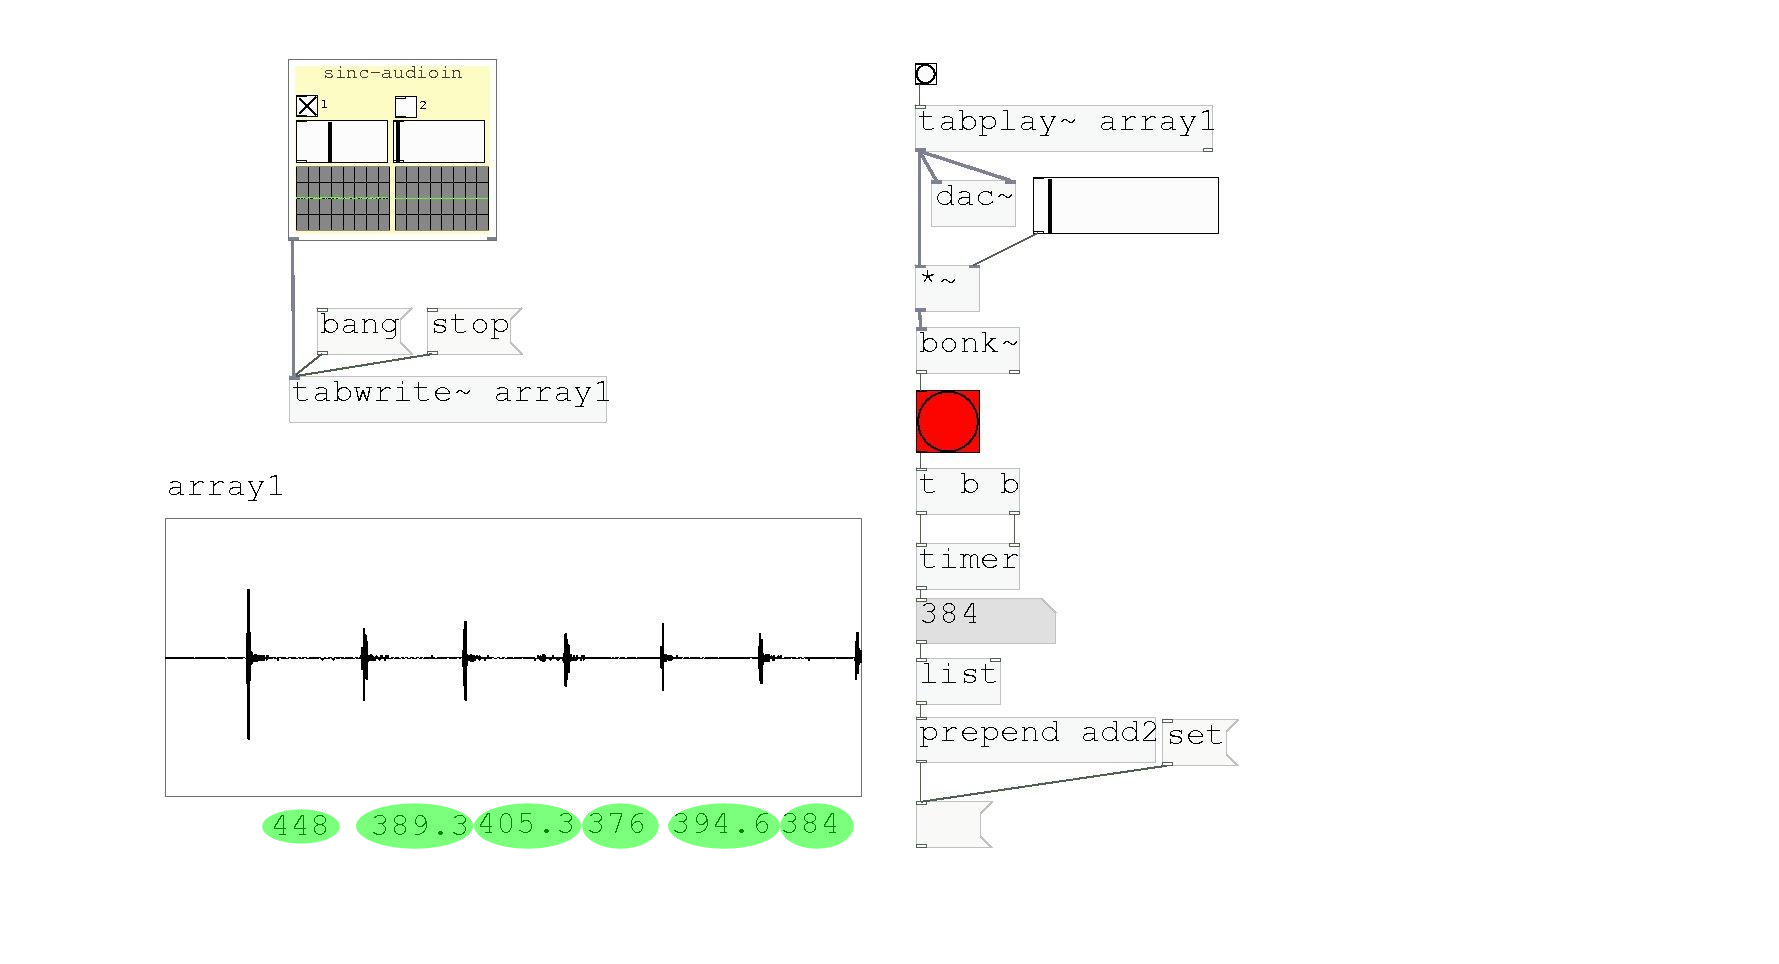
\includegraphics[scale=.4]{ex-ritmo1}
\caption{ritmo estável}
\label{ex-ritmo1}
\end{figure}

\begin{figure}
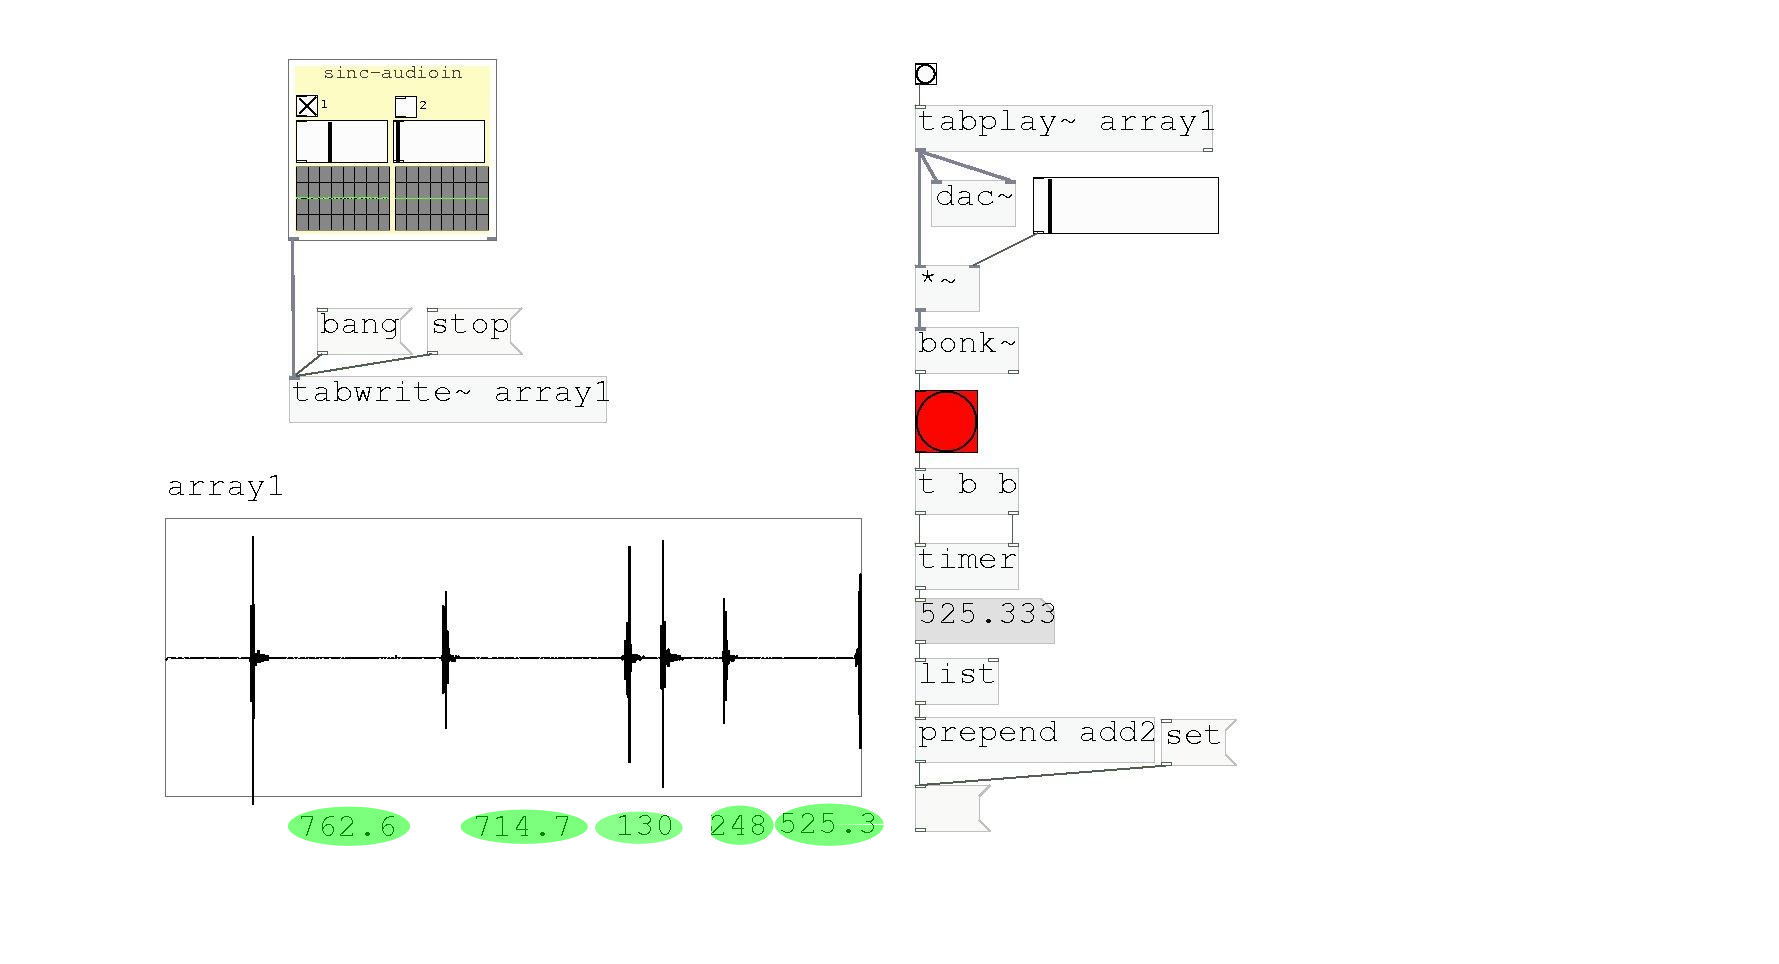
\includegraphics[scale=.4]{ex-ritmo2}
\caption{ritmo instável}
\label{ex-ritmo2}
\end{figure}

\begin{figure}
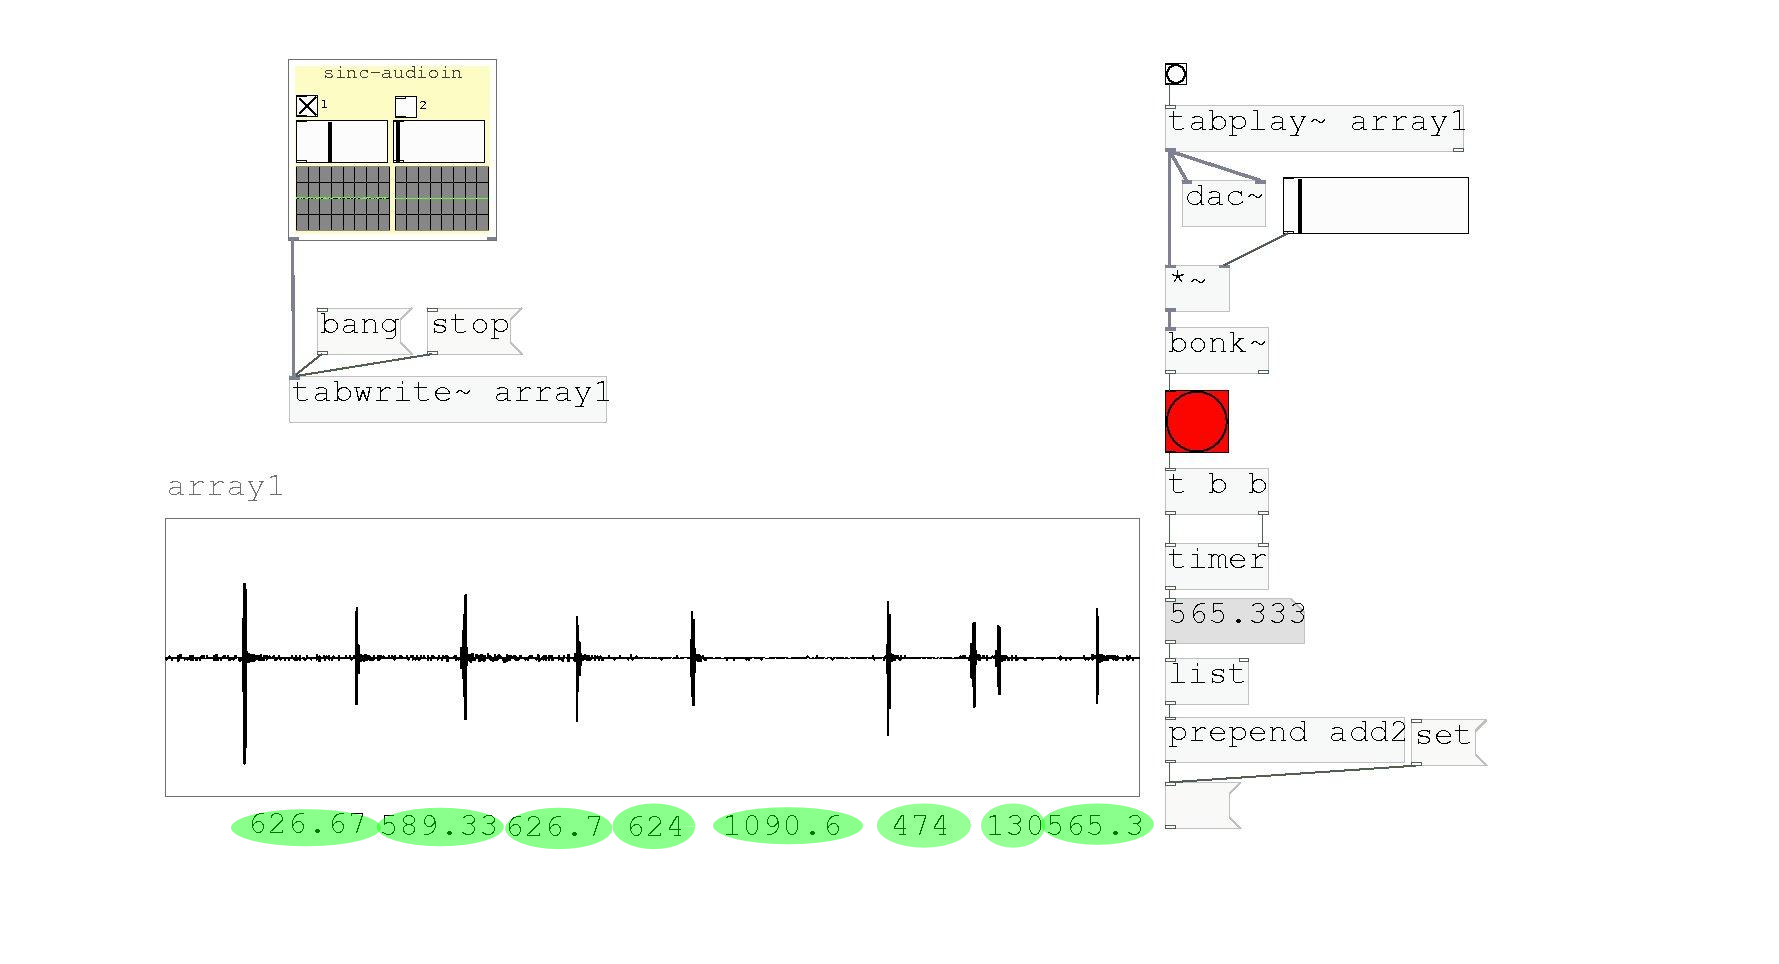
\includegraphics[scale=.4]{ex-ritmo3}
\caption{ritmo estável e instável}
\label{ex-ritmo3}
\end{figure}


A técnica básica de análise rítmica em Pd, se dá através do uso do objeto [timer].
O objeto [timer] mede a distância em milisegundos entre "bangs' que chegam pela entrada
da esquerda em relação ao que chega pela entrada da direita.%% aqui mostrar o básico do timer embasado pelo Rowe


Um músico humano sempre realiza micro-variações de tempo e andamento.
Na figura \ref{ex-ritmo1} vemos uma incidência de ataques mantendo uma relação de estabilidade
de durações. Enquanto que na figura \ref{ex-ritmo2} vemos uma relação mais instável
entre as durações. Já na figura \ref{ex-ritmo3} vemos um padrão que se mantém estável e 
muda para um comportamento de instabilidade de durações. Um dos desafios da pesquisa
foi estabelecer uma forma do programa conseguir classificar a estabilidade de cada nova duração em relação
as anteriores.

No patch da figura \ref{[sinc-calc-ritmo]} é apresentado um método de classificação de estabilidade
de durações entre notas. Primeiro são calculadas as distâncias entre cada ataque
sonoro, depois filtrado em [pd filter-range] e colocado em uma tabela dinâmica em
[pd last-x]. O tamanho da tabela sempre pode ser redimensionado em tempo-real através
da variável \textit{0-buffer-size} então é calculado ao mesmo tempo a média geométrica
e a média aritmética e os resultados são executados na expressão definida por uma
divisão da média geométrica pela média aritmética. %% isso poderia ser definido em notação matemática :)


A divisão da média geométrica pela média aritmética pode ser definida pela expressão

\begin{equation}
\frac{n\sqrt[n]{a1.a2....an}}{a1+a2+...an} 
\end{equation}  

Essa expressão é calculada a cada nota que chega, onde n é o tamanho do buffer.
O resultado desse cálculo devolve um valor numa escala de 0 a 1.
Esse valor representa o índice de instabilidade rítmica da última duração entre 2 notas,
comparado com as últimas "n" durações.
Nesse resultado dessa divisão é aplicado um filtro com [moses] onde se pode calibrar
a sensibilidade do valor do índice final.


\subsubsection{Objeto [sinc-densidade]}

%densidade-ritmica.pd em /abs


Densidade rítmica é o índice que mede a quantidade de eventos sonoros
dentro de espaços de tempo. Serve como ferramenta de análise e pode funcionar
como um parâmetro estrutural em um sistema de aálise musical mais completo.


\begin{figure}
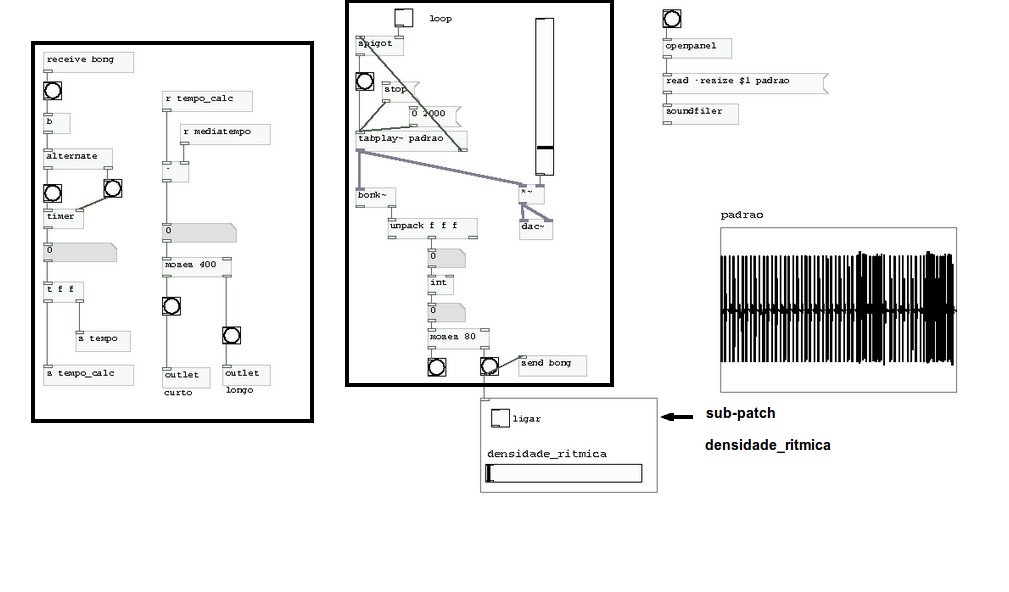
\includegraphics[scale=.5]{prot5b}
\caption{captação de ataques com [bonk\texttildelow] e categorização entre ``curtos'' e ``longos''}
\label{prot5b}
\end{figure}

Os primeiros passos na implementação de um mecanismo de análise de densidade podem ser vistos na figura \ref{prot5b},
onde na área central, aparecem um leitor de samples [tabplay\texttildelow] lendo um arquivo de
áudio e enviando o fluxo de áudio para o objeto [bonk\texttildelow]. A saída de [bonk\texttildelow] é filtrada
pelo objeto [moses] que pode ter um número de corte variável, sendo flexível a diferenças
de volume em diferentes momentos,lugares ou fontes sonoras .

Ainda na figura \ref{prot5b}, a seção da esquerda mostra uma maneira de classificar as durações
entre ataques de notas em longas ou curtas, possibilitando uma classificação básica,
que vai possibilitar a criação de padrões rítmicos de combinações entre longos e curtos.
Nesse caso também o limite entre longo e curto é dado por [moses] que pode ser redimensionado
em tempo-real. 

\begin{figure}
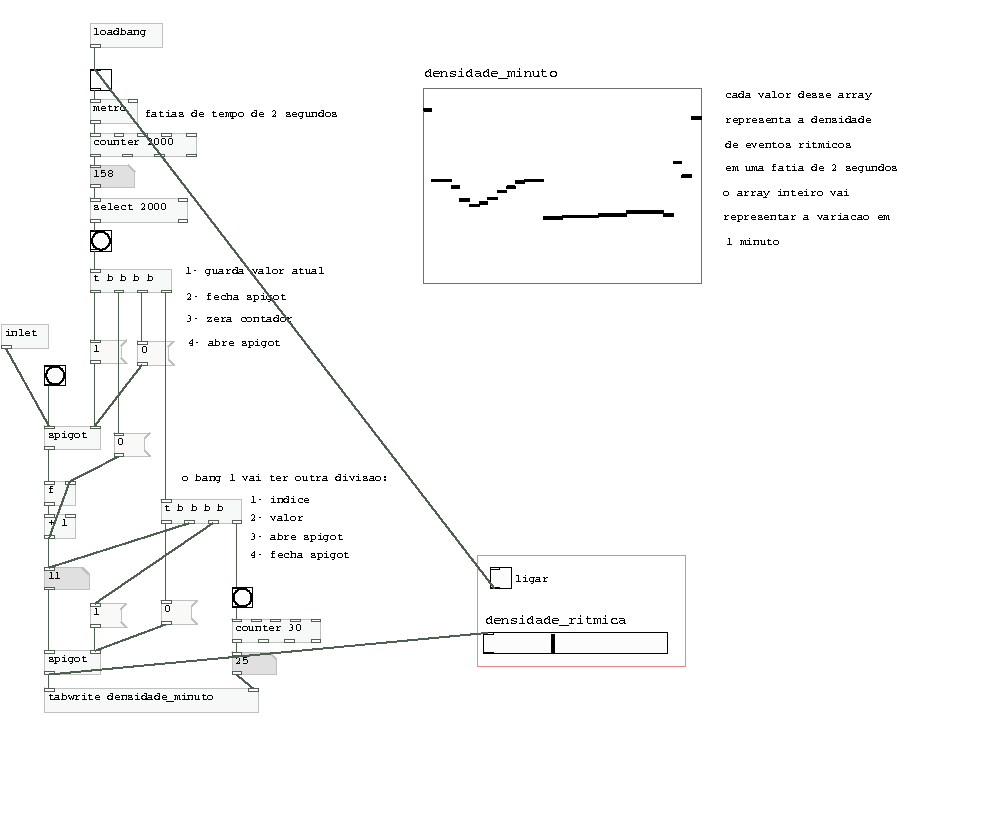
\includegraphics[scale=.75]{prot5c}
\caption{sub-patch [densidade ritmica]}
\label{prot5c}
\end{figure}


Na \ref{prot5c} vemos o conteúdo interno do sub-patch [densidade-ritmica], onde é realizadas
contagens de quantos ataques de eventos sonoros acontecem a cada 2 segundos de tempo.
Densidade rítmica é um bom índice global de controle dos eventos sonoros por um instrumentista.
A maneira de uso desse índice se transforma de um controle rítmico prático para um
músico treinado.





\subsection{Análise de timbre}


\subsubsection{[bonk\texttildelow]}

%% colocar biblio; Miller (Real-time audio analysis tools for Pd and MSP) - 98

O objeto [bonk\texttildelow] possui um sistema interno de classificação
e comparação de amostras de áudio. Essa propriedade possibilita, por exemplo, 
uma situação de acompanhamento interativo para uma instrumentação de 
percussão múltipla.


\begin{quote}
Também é possível pedir para bonk testar qualquer novo ataque 
contra um menu de ataques pré-gravados a fim
de adivinhar qual dos vários instrumentos possíveis foi
responsável pelo novo ataque. Para fazer isso, primeiro temos
que armazenar modelos espectrais para cada um dos instrumentos.
Depois disso, qualquer novo ataque é comparado com o
daqueles armazenados e a correspondência mais próxima é relatada. 
A subjacente suposição de que há realmente alguma
repetibilidade dos envelopes espectrais de ataques de
instrumentos de percussão, certamente não é verdade no mundo real, mas é interessante saber quais
tipos de instrumentos bonk pode identificar desta forma
e quais não. \footnote{It is also possible to ask bonk to test any new at-
tack against a menu of pre-recorded attacks in order
to guess which of several possible instruments was
responsible for the new attack. To do this, first we
store spectral templates for each of the instruments.
Thereafter, any new attack is compared with the
stored ones and the closest match is reported. 
Theunderlying assumption, that there is actually some
repeatability in the spectral envelopes of attacks of
percussive instruments certainly doesn't hold true in
the real world, but it is interesting to learn which
sorts of instruments bonk can identify in this way
and which it can't.} \cite{bonk}
\end{quote}

O objeto [bonk\texttildelow] pode funcionar detectando
ataques em tempo-real retornando um bang para cada ataque 
na saída esquerda. Ou então pode alternar entre dois estágios:
"learn" e "forget" que são enviados como mensagem na entrada de 
[bonk\texttildelow]. Outras mensagens posicionam outros
parâmetros como por exemplo "minvel", para mínima amplitude de offset
para retornar uma detecção de ataque.
Se for enviada uma mensagem com "learn 10",
o objeto irá aguardar dez notas consecutivas do mesmo instrumento.
O resultado da comparação interna é retornado pela saída da direita.



\subsubsection{timbreID}

\begin{figure}
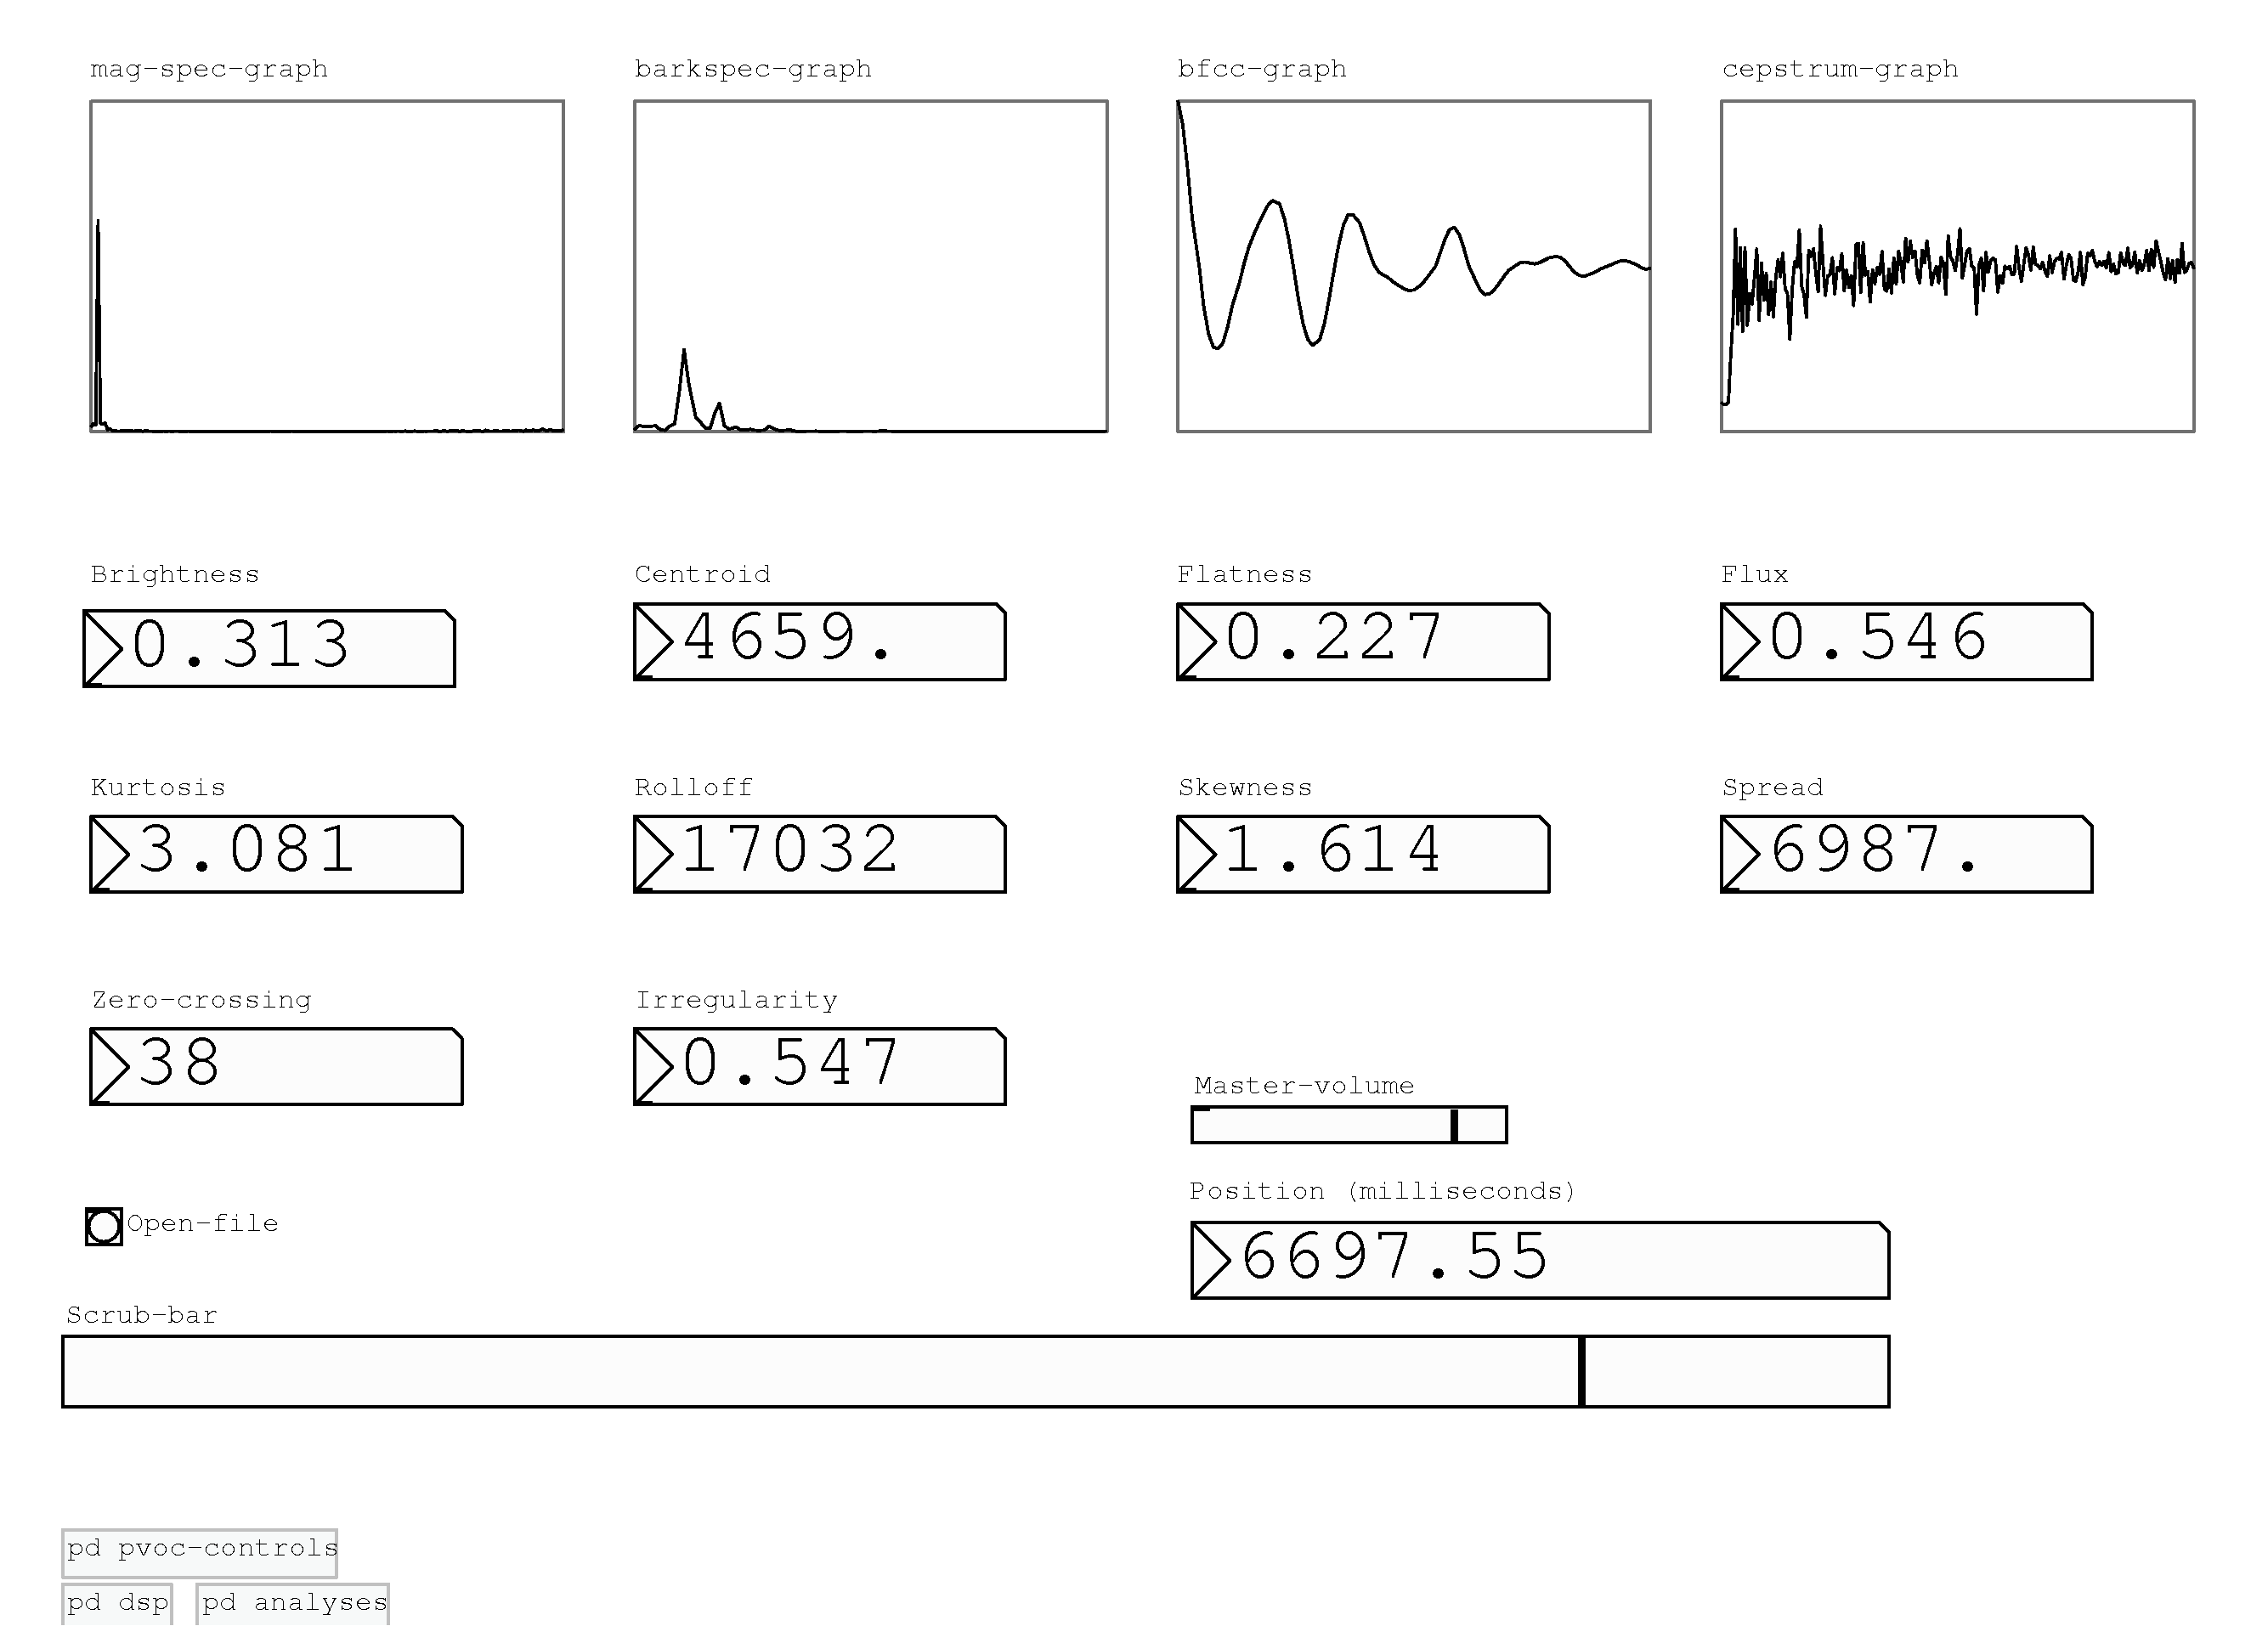
\includegraphics[scale=.5]{audio-features}
\caption{timbreID - audio-features}
\label{audio-features}
\end{figure}

\begin{figure}
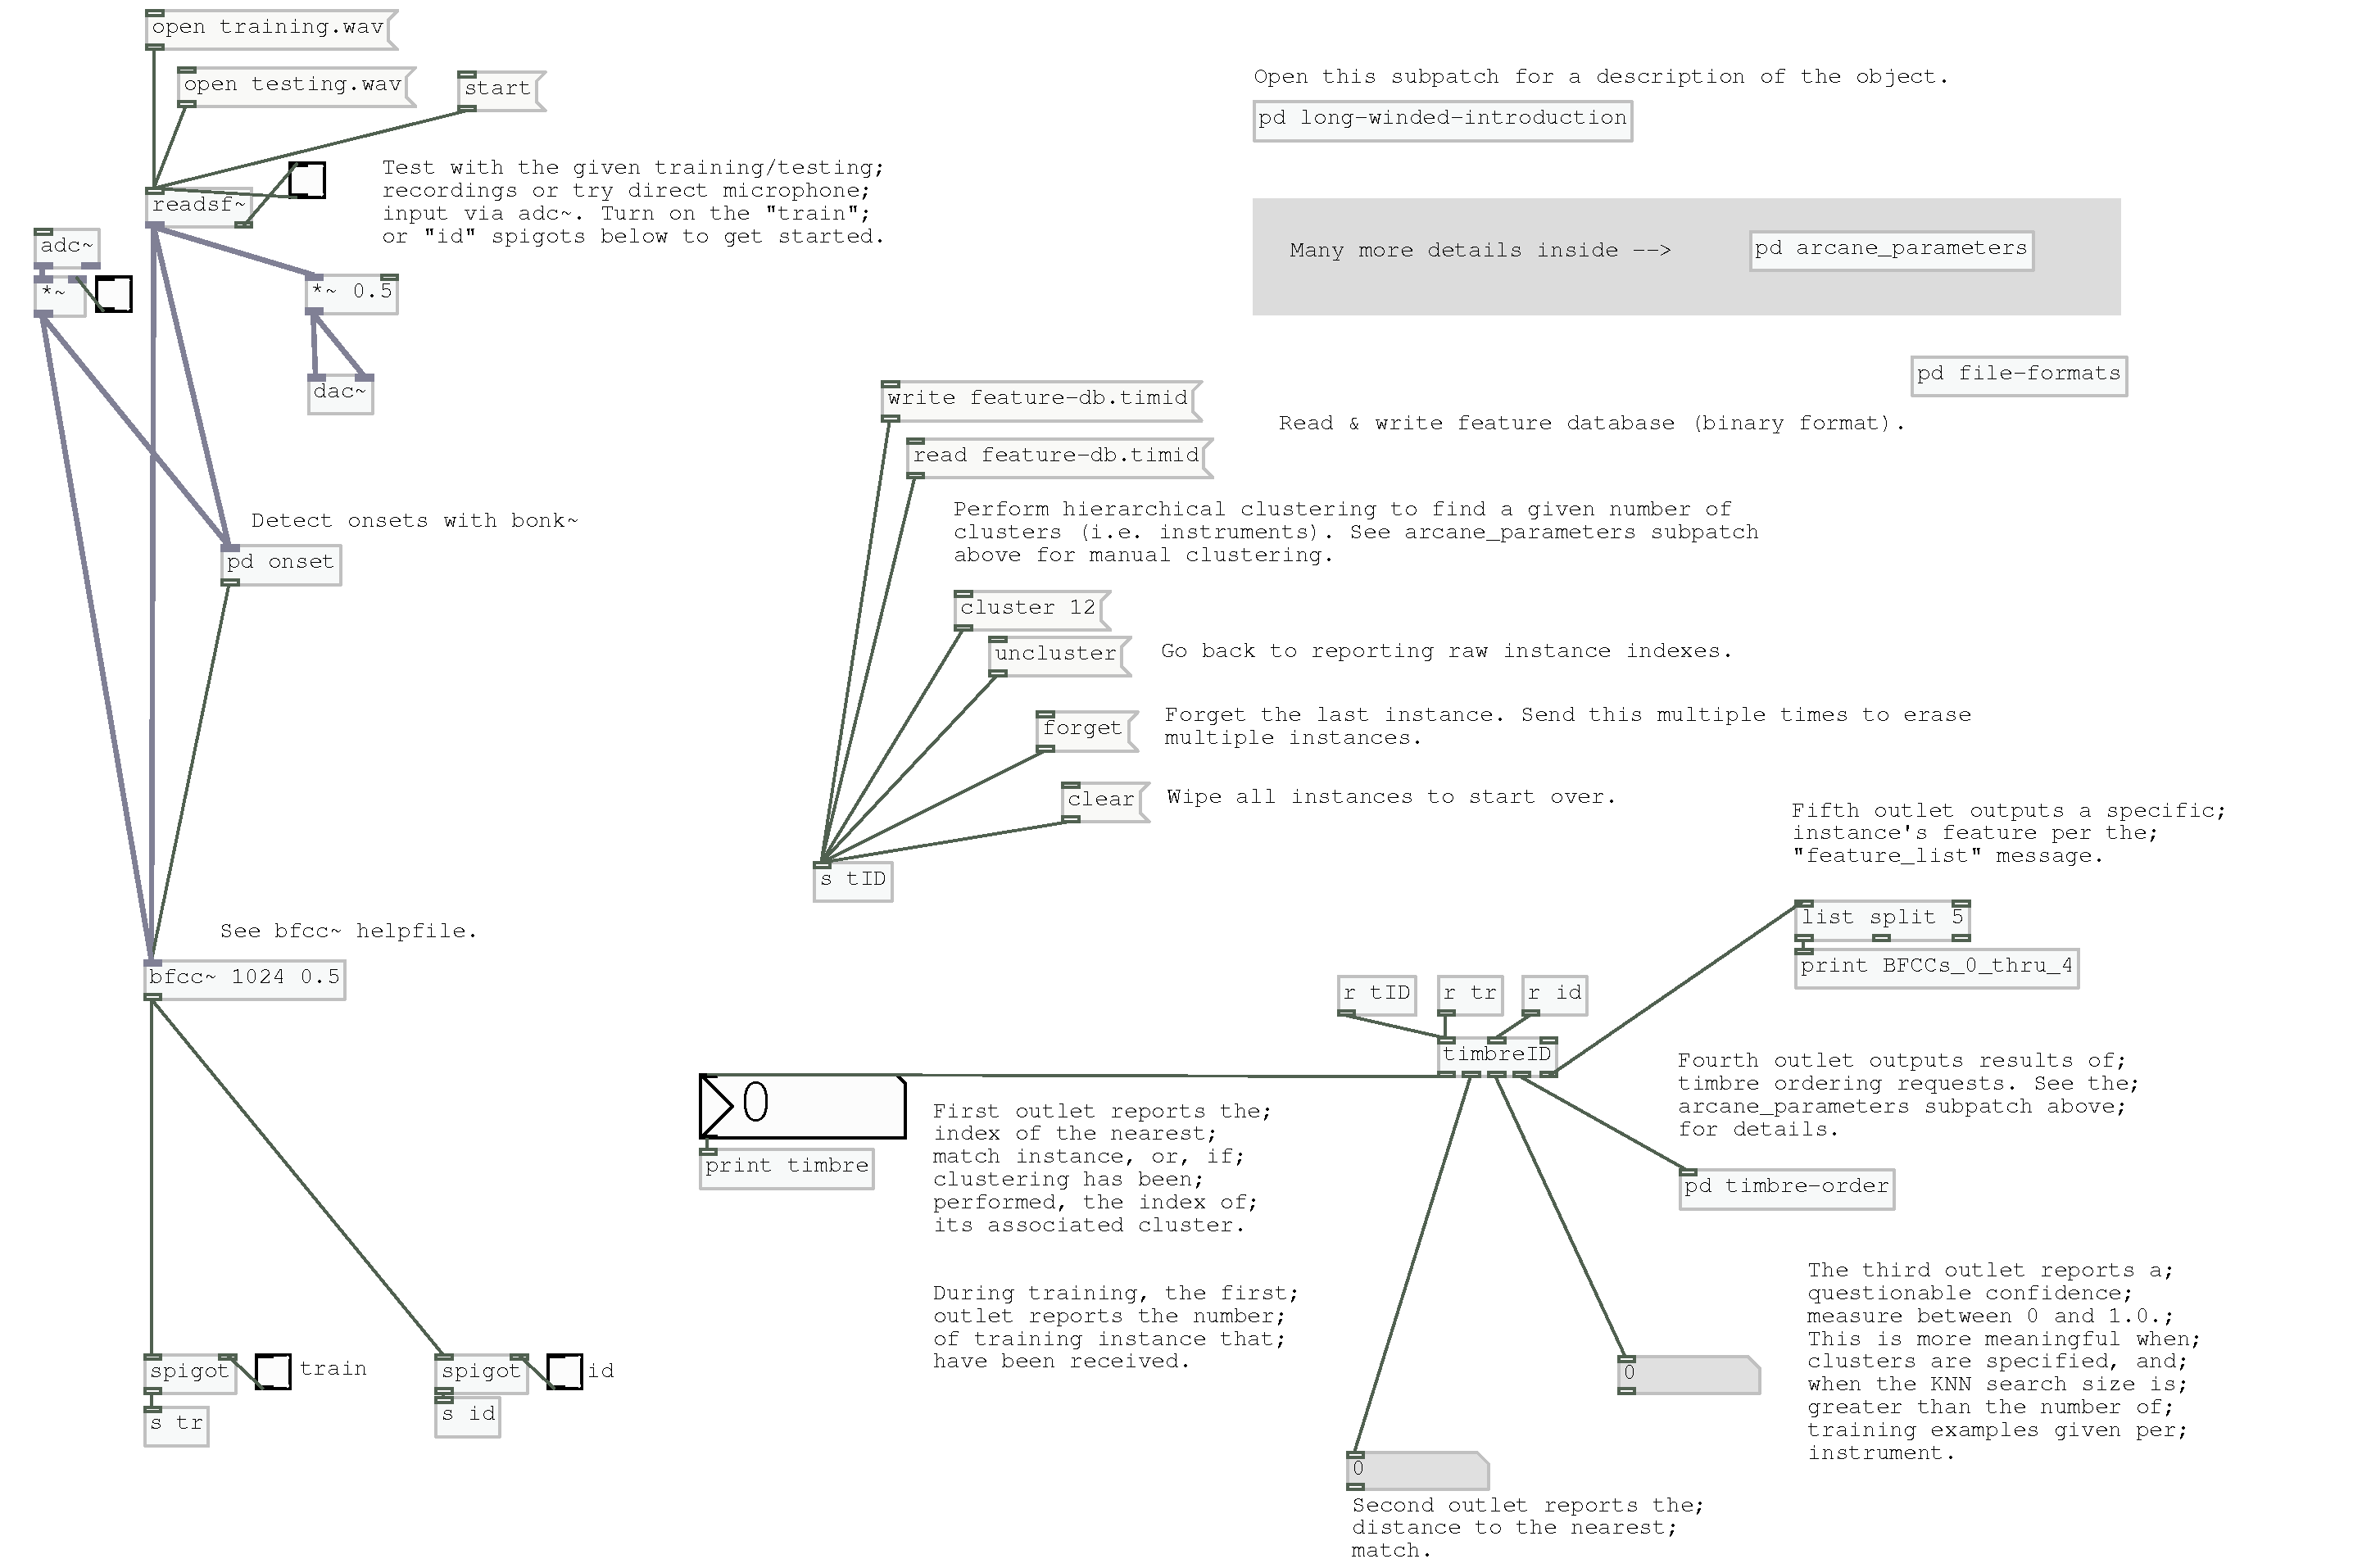
\includegraphics[scale=.5]{timbreid}
\caption{timbreID}
\label{timbreid}
\end{figure}

\begin{figure}
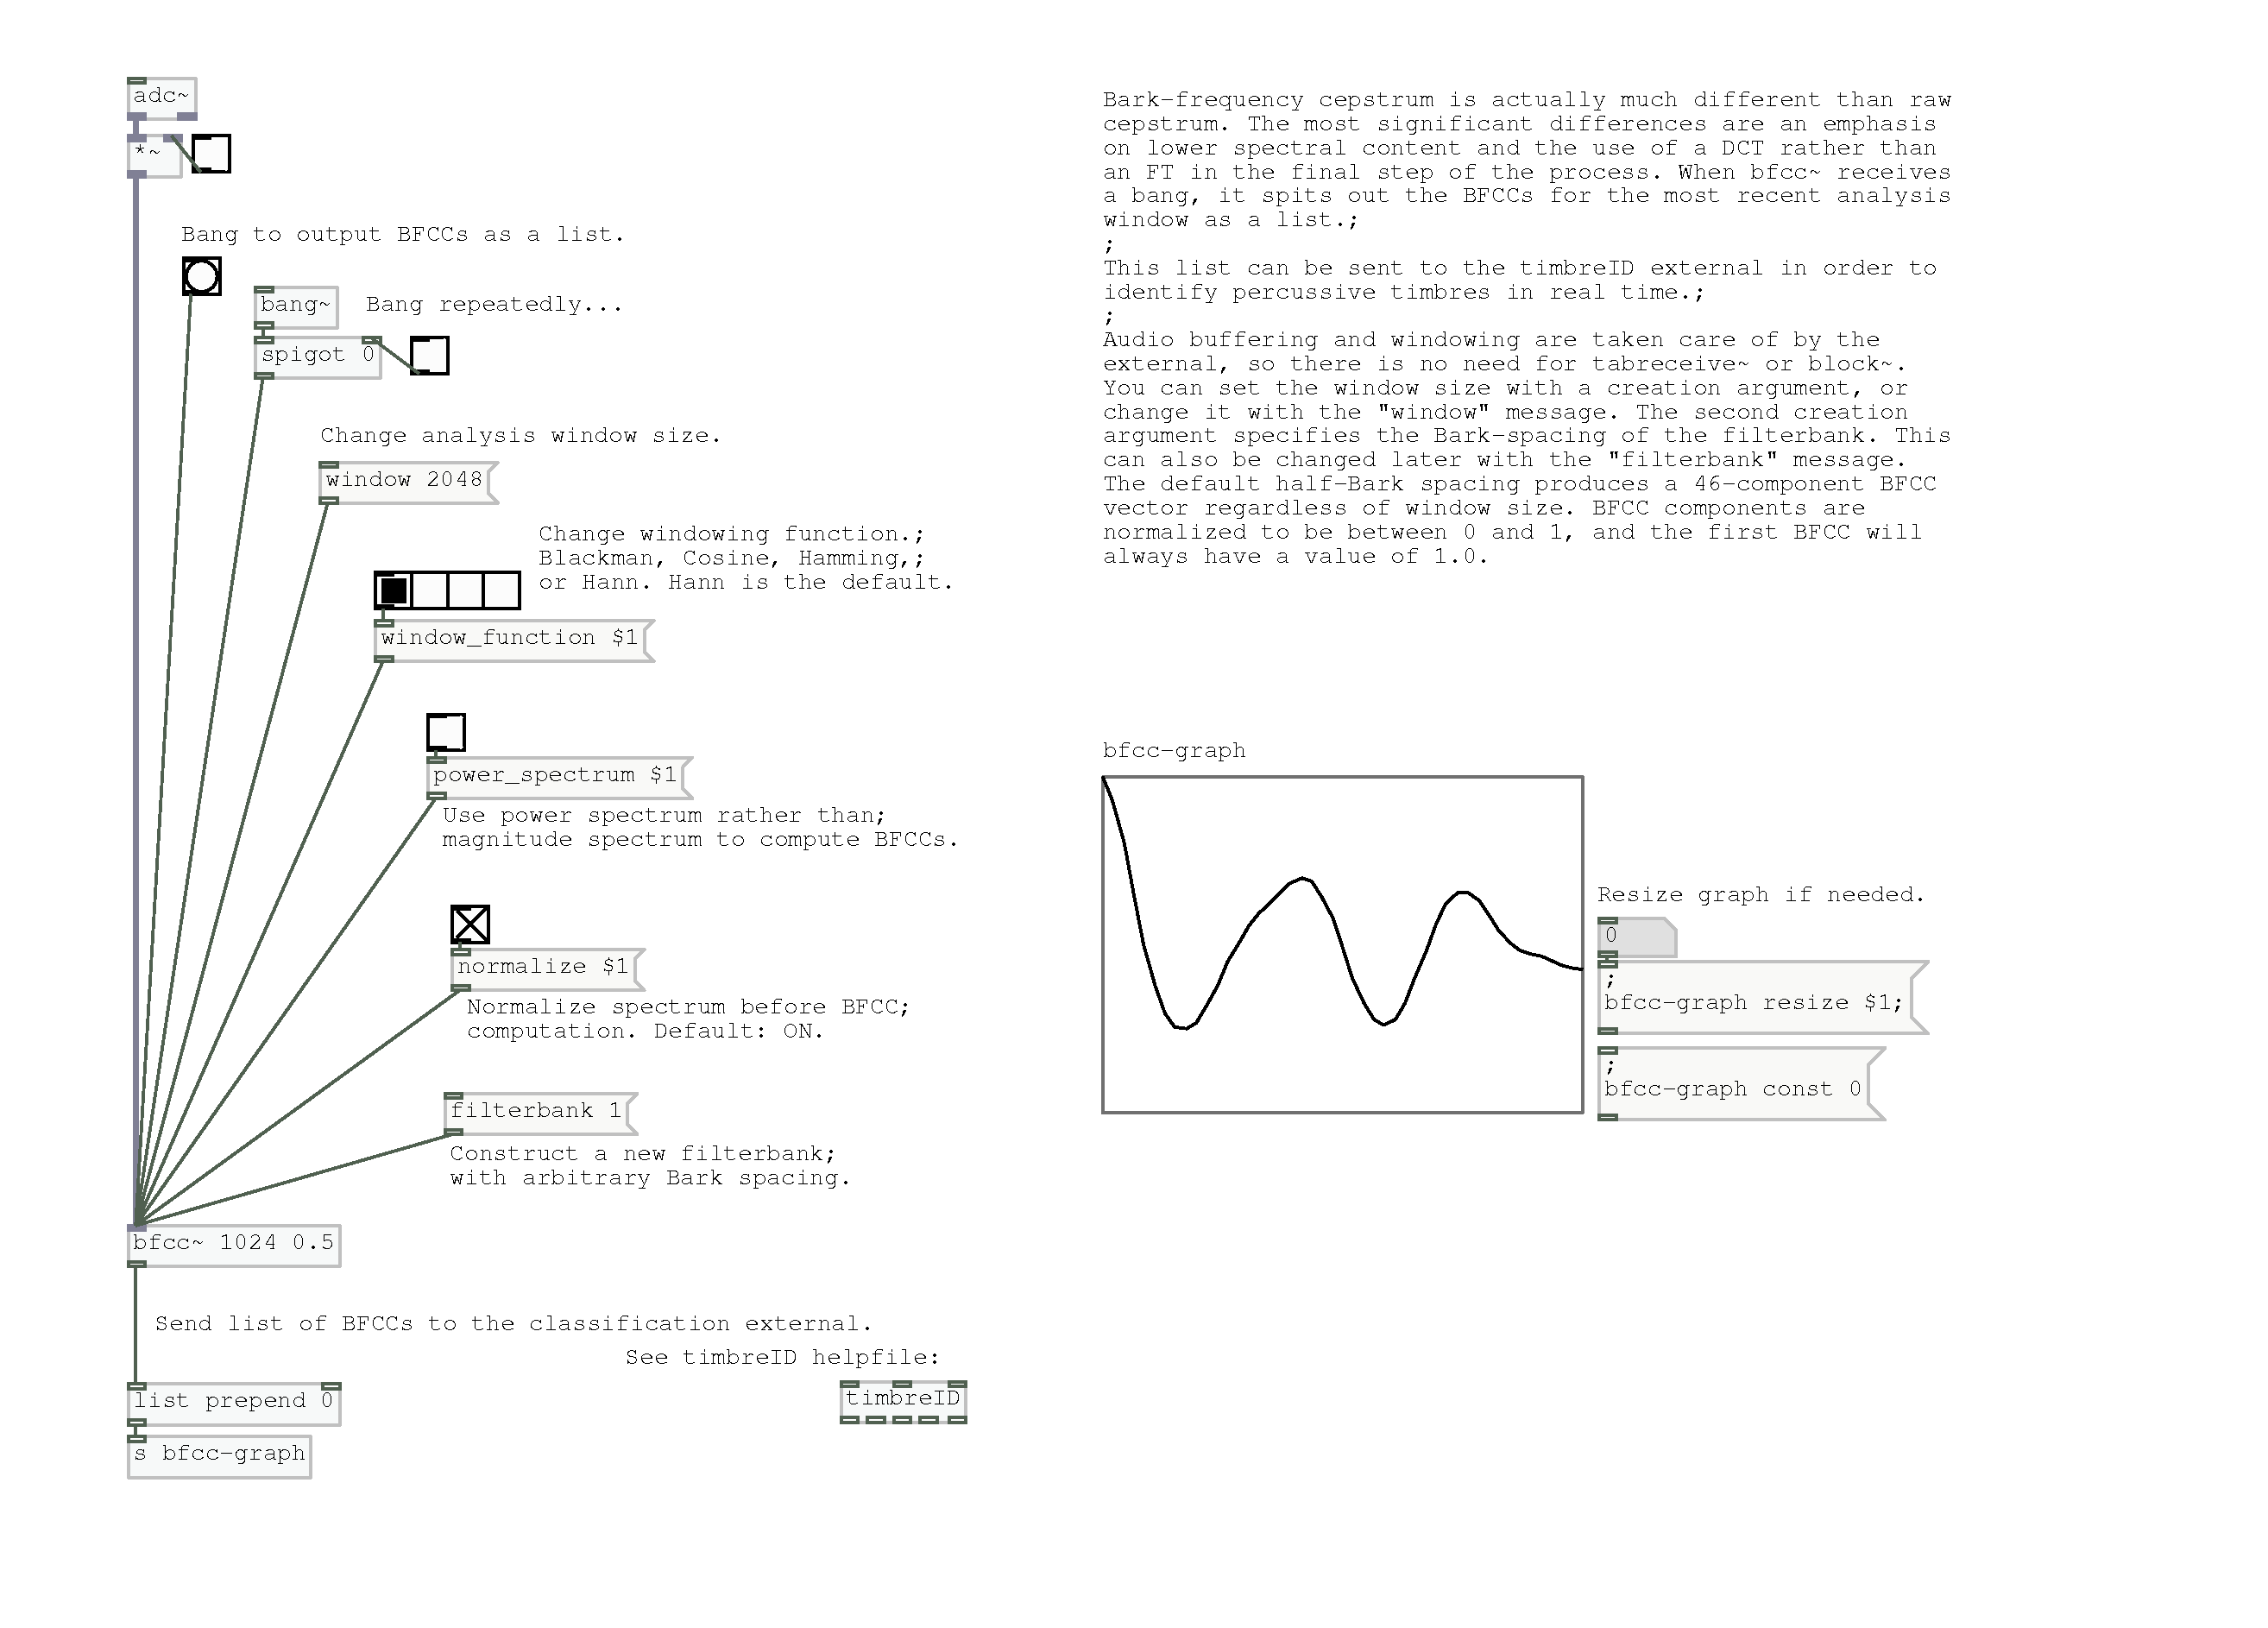
\includegraphics[scale=.6]{bfcc}
\caption{timbreID - bfcc}
\label{bfcc}
\end{figure}

\begin{figure}
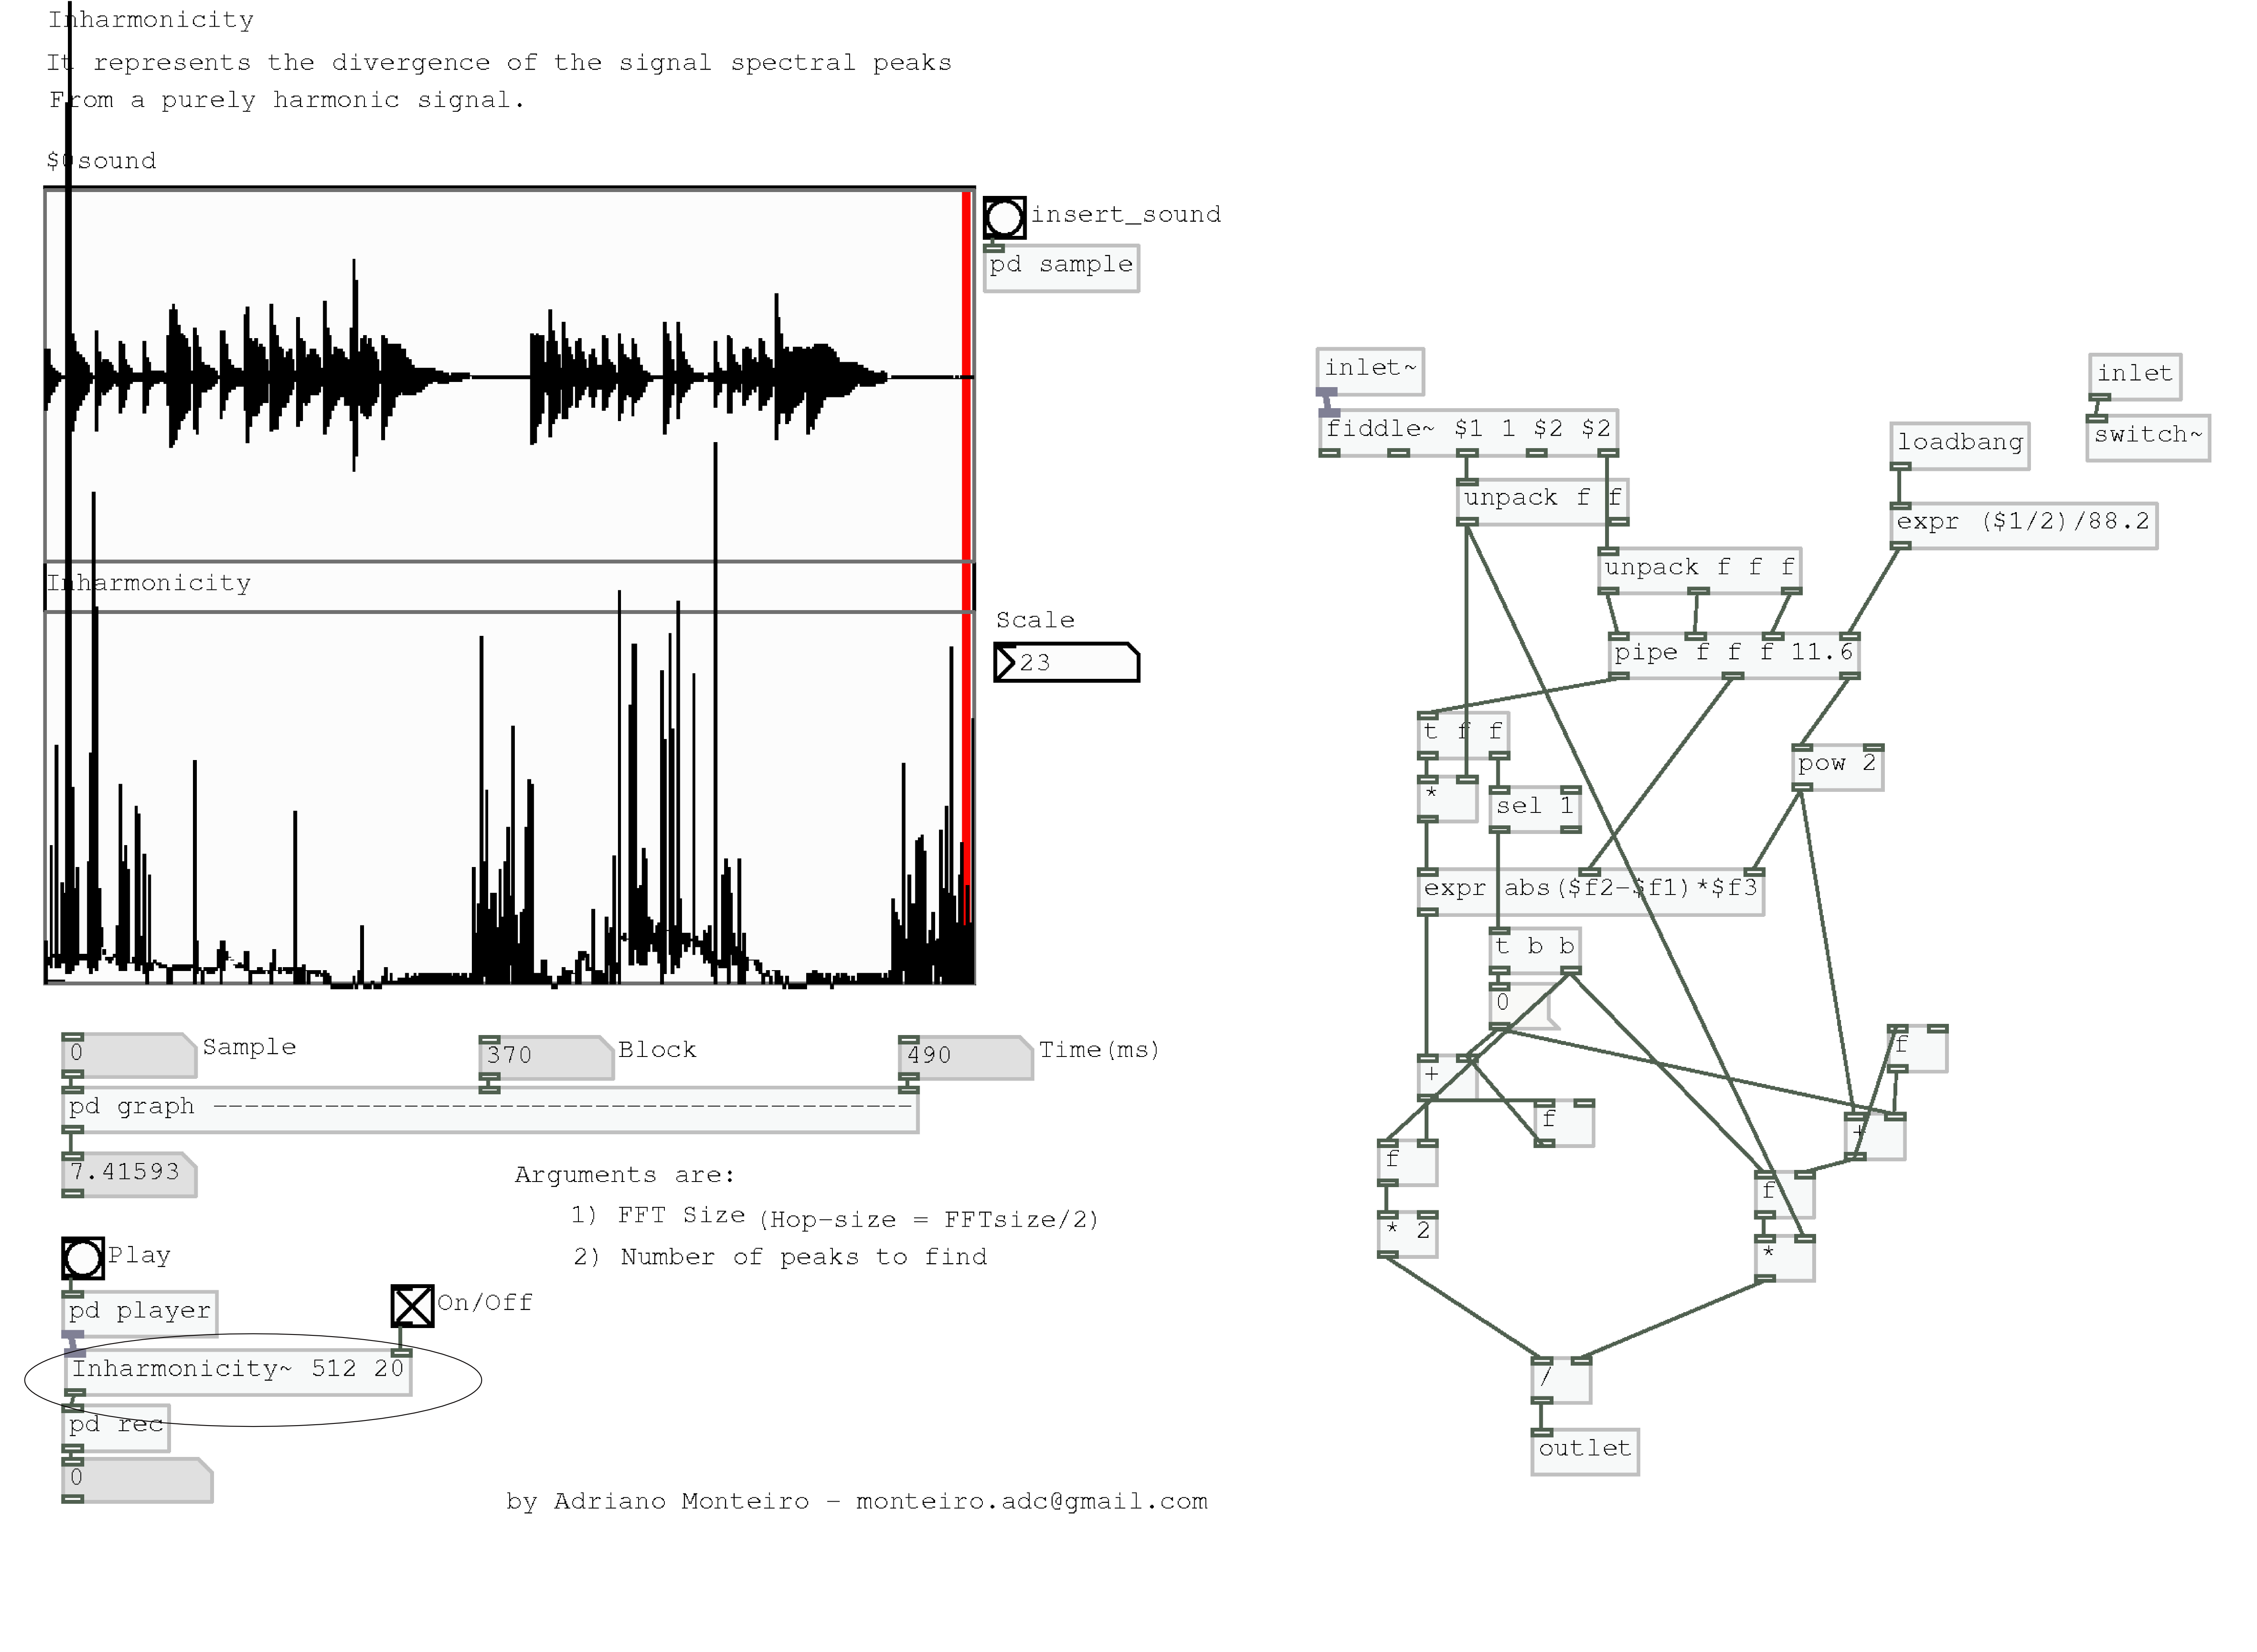
\includegraphics[scale=.28]{pdescriptor}
\caption{PDescriptors - [Inharmonicity\texttildelow]}
\label{pdescriptor}
\end{figure} 


Quando se acessa aos dados puros de um fluxo de áudio precisamos de 
métodos específicos para filtrar esses dados. Uma densa bibliografia
tem sido desenvolvida sobre algoritmos de busca e filtragem de dados de
análise FFT. Cada algoritmo é especializado em algum aspecto, seja de
estimativa de frequência fundamental, ou de comportamento espectral da fonte sonora,
como por exemplo, estimativa se determinado trecho é uma nota com articulação diferente
ou um ruído indesejado.
Pode-se dizer que a filtragem dos dados de análise espectral é um importante
núcleo dentro da pesquisa em música interativa e computação musical. Nessa seção
serão comentadas algumas ferramentas que demonstram o estado da arte da análise de 
áudio em tempo real, que permitem um maior refinamento na detecção de parâmetros
sonoros em projetos de música interativa.

Nese sentido, além dos dados puros da FFT feita com o objeto [rfft\texttildelow],
destacamos duas bibliotecas externas de Pd que compreendem diversos algoritmos
diferentes de análise. A primeira biblioteca é a 
timbreID \cite{brentcepstral} desenvolvida por William Brent e compreende uma série de objetos
implementados em C e possui uma boa eficácia em processamento. A timbreID possui 
quatorze objetos de análise espectral cada um em versão estática e tempo-real, com a diferença
de que a versão em tempo-real processa áudio em vez de valor de amostra. Além
de um objeto classificador [timbreID]. Na figura \ref{timbreid} temos
uma visão geral de um dos algoritmos de análise do objeto  [bfcc\texttildelow], baseado na 
análise Cepstral enviando dados para o classificador [timbreID]. Na figura \ref{bfcc} podemos
ver em detalhe o funcionamento de [bfcc\texttildelow].

\begin{quote}
Bfcc\texttildelow é o objeto de análise \textit{cepstral} mais desenvolvidp, utilizando a escala \textit{Bark} 
mais bem pesquisada, em vez de \textit{Mels} para a ponderação do espectro. O desempenho é apenas ligeiramente melhor do 
que MFCC\texttildelow. A coisa mais notável sobre estes cepstral externs é a flexibilidade que proporcionam no 
que diz respeito à construção do de banco de filtros. A escolha de um valor ideal de \textit{Bark} ou \textit{Mel} 
 pode ter um impacto real sobre o quão relevante são esses parâmetros na classificação de um som em relação a outro
\footnote{Bfcc\texttildelow is the most developed cepstral external, using the more thoroughly researched Bark scale rather than mels for 
the spectrum weighting. Performance is only slightly better than mfcc\texttildelow. The most noteworthy thing about these cepstral 
externs is the flexibility they provide with respect to filterbank construction. The choice of a specific Bark- or 
mel-spacing can have a real impact on how relevant the features are in classifying one sound set vs. another.}. 
\cite{brentcepstral}
 
\end{quote}


Uma das vantagens da timbreID é a flexibilidade de parametrização. A biblioteca é dividida
entre objetos externos para implementação de cada algoritmo e um objeto responsável pela
classificação dos resultados dos algoritmos. O objeto de classificação ([timbreID]) aceita
listas de características timbrísticas e tenta encontrar a melhor correspondência entre cada 
característica do áudio de entrada e instâncias estocadas dos dados treinados.
Listas de características mandadas para a entrada da esquerda são processadas pela função
"train" (em formato de mensagem). Isso fornece exemplos das características que sobre as quais
futuras comparações serão baseadas. Uma vez que uma base de dados de treinamento é criada, ela
pode ser salva em um arquivo .timid com o método "write", e mais tarde recuperado com o método
"read". Outros formatos de saída são .txt, .mat (para uso com os programas MATLAB ou Octave)
e ARFF (para uso com o ambiente WEKA).

A segunda entrada do objeto [timbreID] recebe listas de características que são comparadas com
aquelas no banco de dados do treinamento e uma correspondência é identificada. As instâncias de 
correspondência são distinguidas pelo índice, por isso, se a correspondência mais próxima for o 
índice 7, o número 7 vai aparecer na primeira saída da esquerda.

Na figura \ref{audio-features} vemos um painel geral com os resultados simultâneos dos quatorze
algoritmos de análise espectral diferentes. Notamos que os quatro objetos superiores retornam resultados em 
listas que são plotadas em arrays, enquanto os demais objetos retornam índices puros.

Outra  biblioteca relevante é a PDescriptors \cite{monteiro} que se tratam
de abstrações de Pd que usam apenas objetos "vanilla" e por isso possui um
grande poder de compatibilidade com diversos projetos. As abstrações
são divididas em características perceptuais, espectrais, harmônicas e temporais, além
de alguma ferramentas de transcrição. Podemos ver a interface do objeto [Inharmonicity\texttildelow]
na figura \ref{pdescriptor}, onde o resultado da análise é plotado no gráfico abaixo da forma de 
onda da fonte, o que facilita a comparação visual, resultando numa boa interface para trabalho de análise de áudio.



\pagebreak 



\section{Análise Humdrum}

  Dentro de um projeto de música interativa, são necessárias informações quantitativas quanto a 
variação de parâmetros musicais pelo músico, como por exemplo quais acordes foram mais usados 
nos últimos 12 compassos.
Nesse sentido o Humdrum é uma boa plataforma de análise simbólica de estruturas musicais. 
Nesse protótipo, procuramos investigar de que maneira podem se conectar as duas linguagens 
com visualização de dados em Gem.
Na \ref{interface} mostramos a visão geral da interface e controle
do protótipo, com a opção de se carregar um arquivo midi, 
que pode ser substituído por arquivos midi gerados em tempo real 
durante uma performance.

% \begin{figure}
% 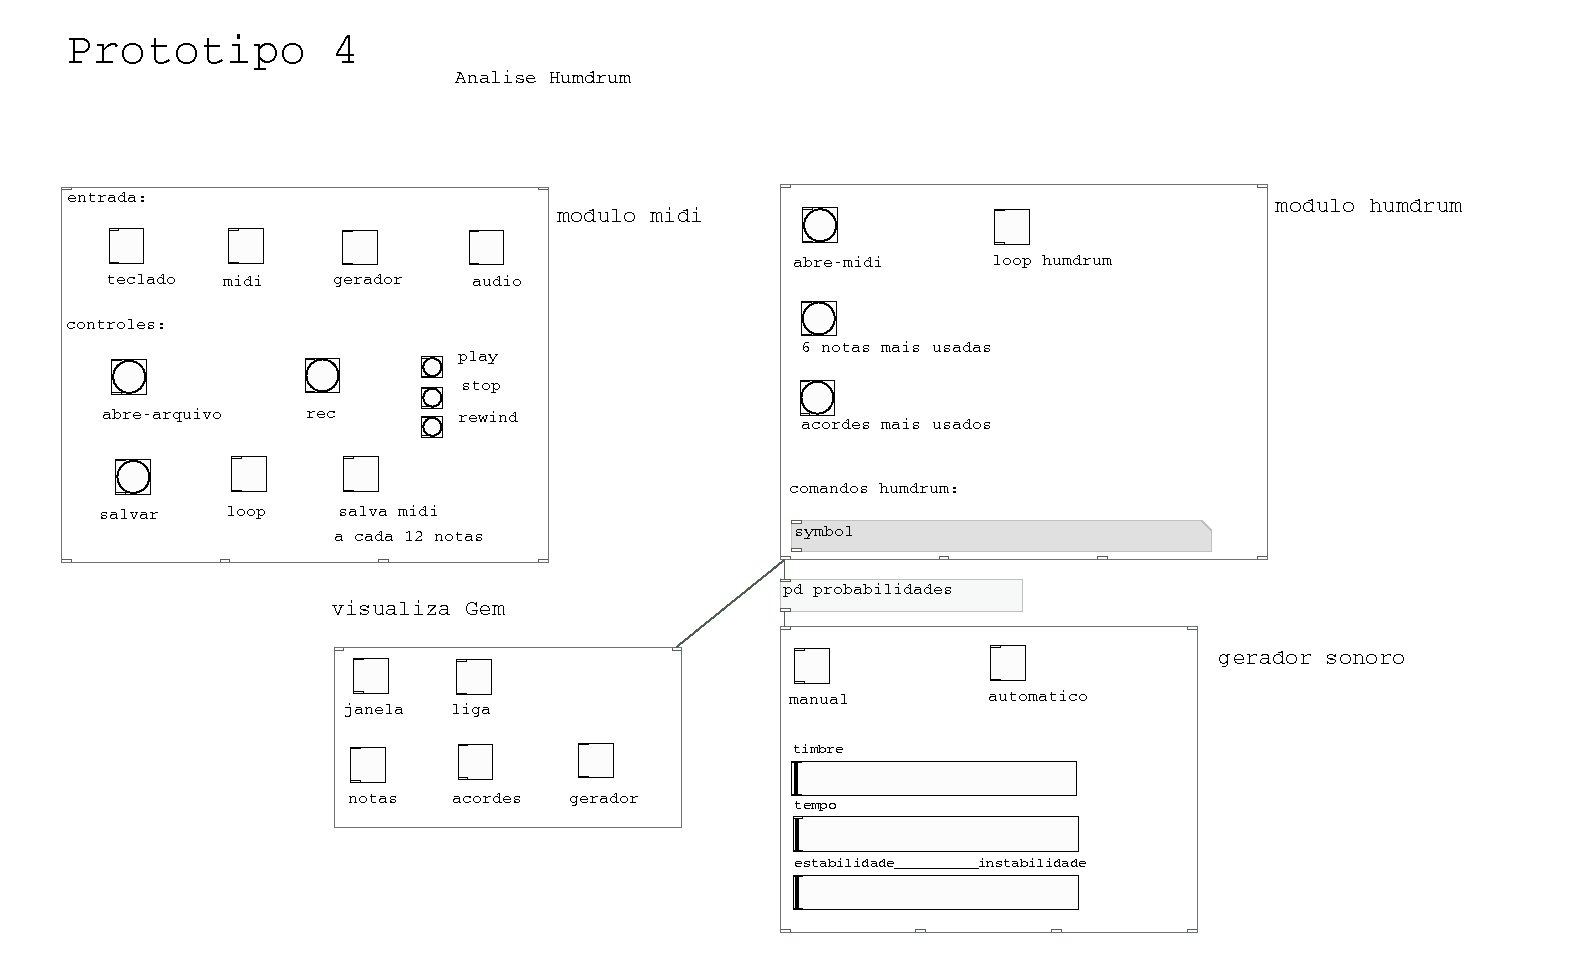
\includegraphics[scale=.5]{prot4}
% \caption{protótipo 4}
% \label{prot4}
% \end{figure}



\begin{figure}
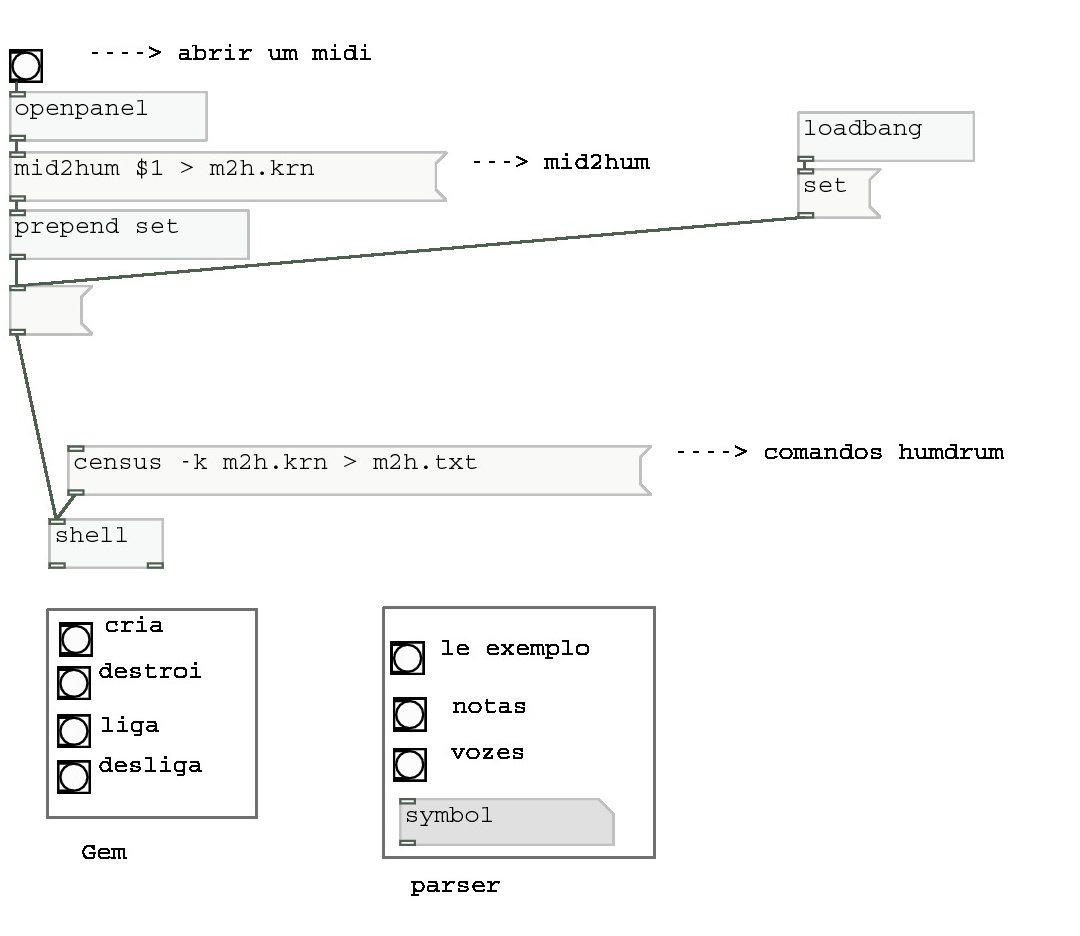
\includegraphics[scale=.7]{interface00}
\caption{interface}
\label{interface}
\end{figure} 

\textbf{Parseando strings no Pd}


O parser funciona em 3 instâncias:

1) Abre-se um arquivo midi com o objeto [openpanel] através
de uma janela de diálogo, o path do arquivo substitui a variável 
dólar 1 como argumento para o programa mid2hum que converte
arquivos midi para o formato kern (.krn), usado pelo humdrum.
\begin{verbatim}
 midi2hum \$1 > m2h.krn
\end{verbatim} 
  O código acima é formatado numa mensagem e enviado ao objeto
[shell] onde converte o arquivo midi e envia o resultado para
um novo arquivo chamado m2h.krn.
 
2) Nessa etapa é onde se aplica os comandos do humdrum ao 
arquivo gerado. No caso o comando
\begin{verbatim}
census -k m2h.krn > m2h.txt
\end{verbatim} 
traz diversas informações sobre o arquivo enviadas para um 
arquivo de texto como por exemplo:
\begin{verbatim}
 HUMDRUM DATA

Number of data tokens:     2510
Number of null tokens:     0
Number of multiple-stops:  470
Number of data records:    2511
Number of comments:        817
Number of interpretations: 301
Number of records:         3629

KERN DATA

Number of note-heads:      2491
Number of notes:           2209
Longest note:              2
Shortest note:             384
Highest note:              gggg#
Lowest note:               FFF
Number of rests:           310
Maximum number of voices:  4
Number of single barlines: 237
Number of double barlines: 0
\end{verbatim} 

3) Nessa parte expomos um método de navegar e procurar por
informações no arquivo de texto. O código usado como modelo,
está assinalado na figura \ref{parser}. O arquivo m2h.txt
é lido pelo objeto [msgfile] e envia uma lista com todo conteúdo
do arquivo para os objetos [list-find] e [list-seek]. Em [list-find]
podemos procurar por um símbolo específico dentro da lista e nos retorna
a posição do símbolo. No caso do código assinalado, vemos o símbolo 
``notes:'' , porém como desejamos o valor de ``notes:'' pegamos a posição
de ``notes:'' na lista e adicionamos um número para acessar o lugar do valor de
``notes:'' na lista. Essa posição é enviada para [list-seek] que retorna o valor ou
símbolo na posição desejada. Como teste escolhemos os parâmetros ``notes:'' e ``voices:'', 
respectivamente número de notas e número de vozes encontradas no arquivo.


\begin{figure}
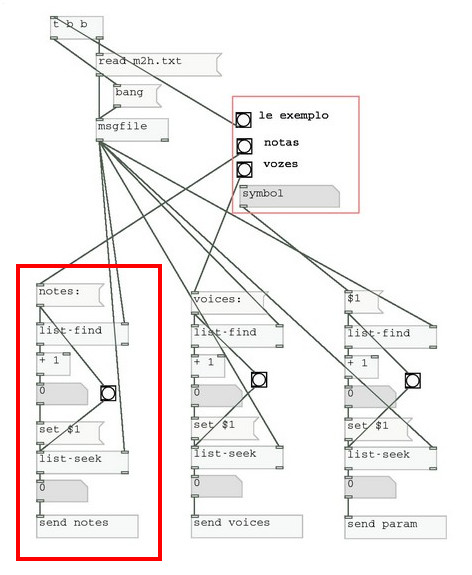
\includegraphics[scale=.5]{parser00}
\caption{parser}
\label{parser}
\end{figure} 


\textbf{Visualização com GEM}


  Os valores de números de notas e número de vozes são visualizados
com objetos da biblioteca Gem (Graphics Environment for Multimedia).
No caso os 2 parâmetros são enviados para 2 cubos 3D onde os valores
são lidos como valores de tamanho dos cubos.



\begin{figure}
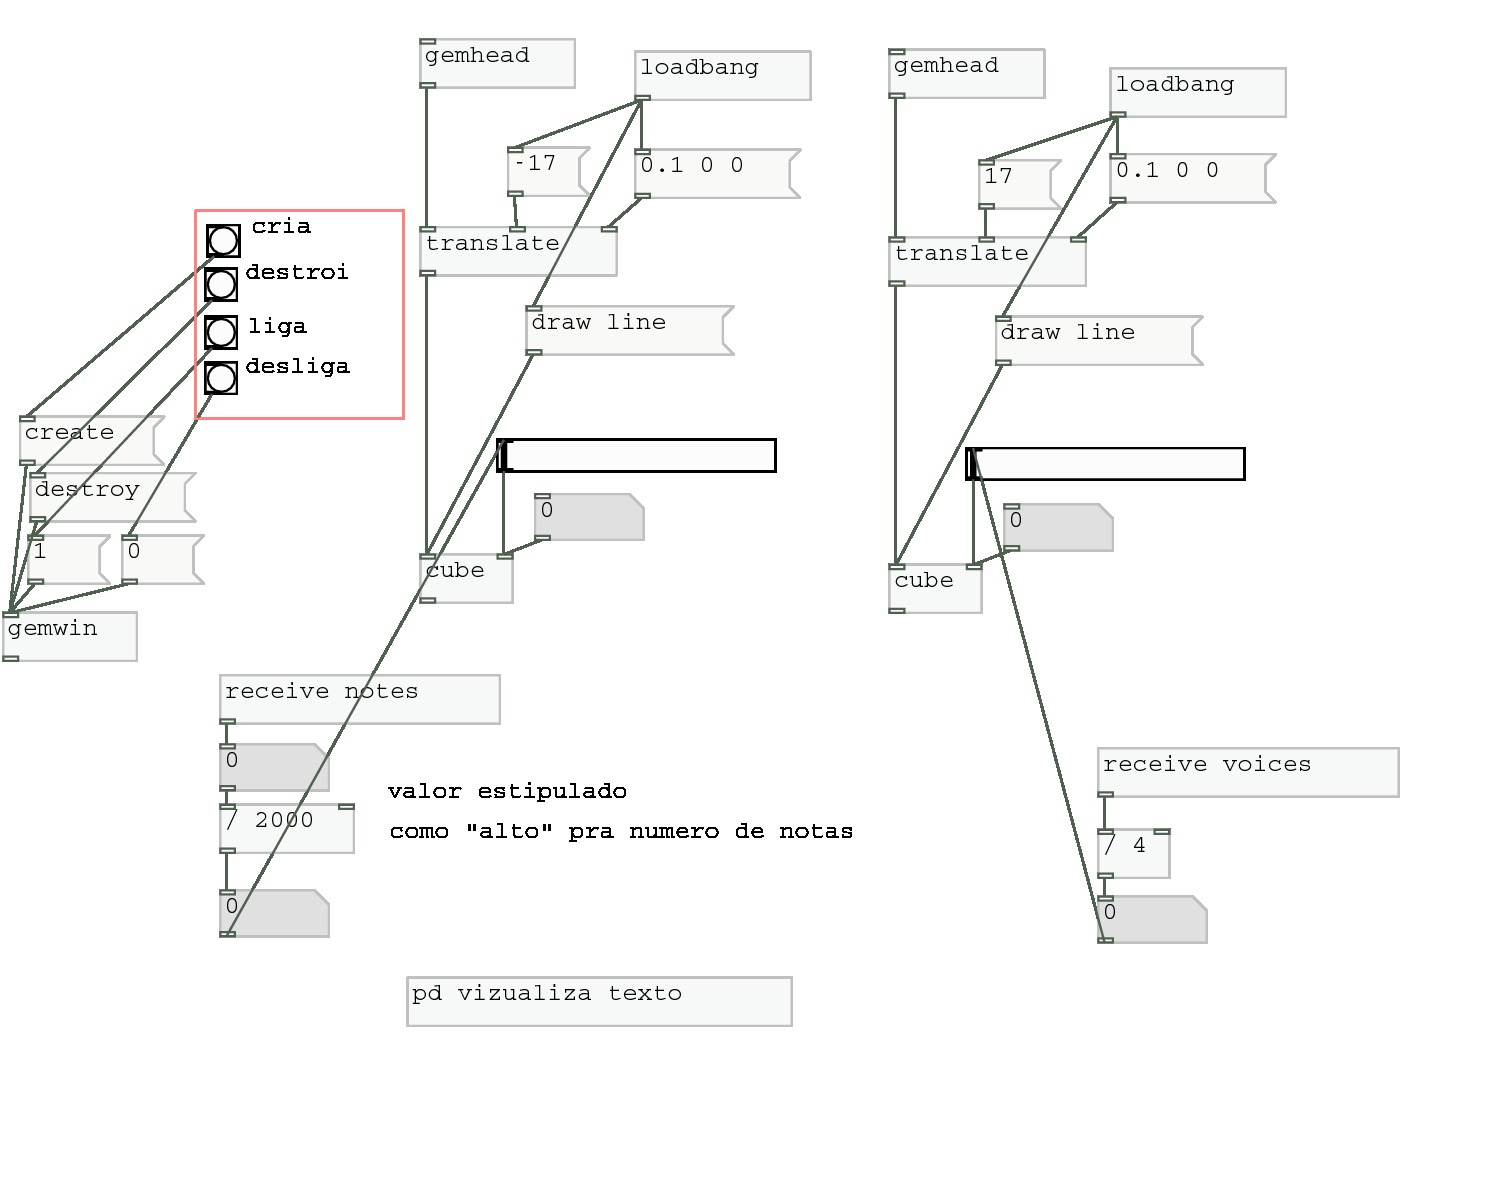
\includegraphics[scale=.5]{gem00}
\caption{GEM}
\label{GEM}
\end{figure} 


\begin{figure}
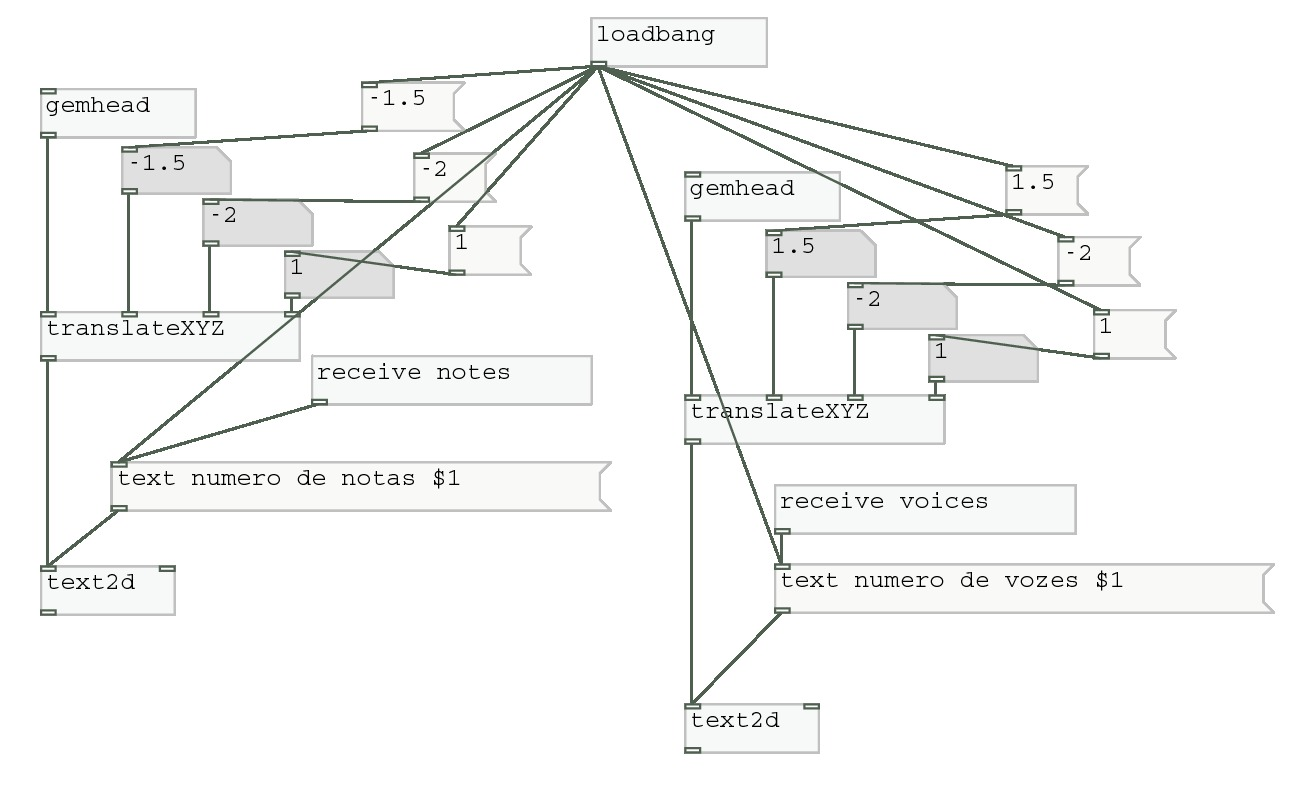
\includegraphics[scale=.5]{gemtexto00}
\caption{GEM texto}
\label{GEM texto}
\end{figure} 



\begin{figure}
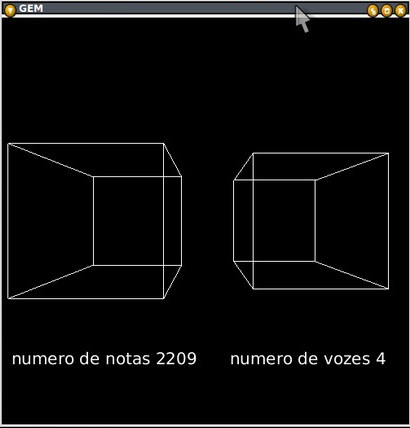
\includegraphics[scale=.5]{gemwin}
\caption{gemwin}
\label{gemwin}
\end{figure} 



  Nesse protótipo, mostramos uma metodologia
simples de unir duas linguagens muito usadas em pesquisa de música.
Essa metodologia é uma maneira clara de como acessar outra linguagem dentro do Pd
enriquecendo as possibilidades da linguagem.


\pagebreak





\section{Geradores MIDI}

%% em primeiro lugar dizer  O QUE SÃO OS GERADORES

Nessa seção serão descritos os geradores MIDI, que
são módulos de composição algorítmica alimentados
por dados da análise da entrada do músico.

Durante a implementação dos geradores de material musical,
procurou-se aliar técnicas de composição algorítmica com
o resultado das análises do áudio de entrada.


A idéia é de ter uma coleção de geradores, capazes
de imitar, simular, seguir ou serem alterados por elementos da performance humana. A análise do áudio
tenta fazer uma descrição da performance e essa descrição
é enviada aos geradores, mediados pelo cenário de interação.
Nesse sentido as análises alimentam os parâmetros dos
geradores, conduzindo o comportamento dos mesmos.



Notadamente alguns trabalhos tem influenciado bastante o desenvolvimento
dos geradores, servindo de ponto de partida para a implementação. Como
por exemplo a biblioteca RTC\footnote{A biblioteca RTC (\textit{Real-Time Composition} 
foi desenvolvida pelo compositor Karlheinz Essl em MAX, a re-implementação
em Pd foi feita por Frank Barchnet, poderemos ver uma visão mais geral
das funcionalidades dessa biblioteca no apêndice} e o método MEPSOM\footnote{
MEPSOM (Método de Ensino de Programação Sônica para Músicos) desenvolvido por
Elói Fritsch é um método que ensina composição algorítmica no ambiente MAX. Alguns
exemplos de MEPSOM foram portados para Pd e podem ser vistos no apêndice}, além
de alguns objetos das bibliotecas PDMTL e Rj.  


Músicos frequentemente separam os aspectos rítmicos, melódicos e de dinâmica
quando estudam performance ou compõe. É comum um instrumentista executar um 
mesmo perfil melódico em diferentes combinações rítmicas e com articulações
diferentes. Muitos métodos de educação musical começam com exercícios rítmicos
para depois incluir exercícios melódicos. Ao implementar os geradores midi
nessa pesquisa, levou-se em conta esses aspectos e decidiu-se manter a separação
entre os domínios do ritmo, melodia e dinâmica. Criando uma relação de funcionamento
desses geradores, possibilitando uma expansão organizada de técnicas de geração.
Na implementação de Sincopa, projetamos 3 objetos que trabalham juntos para
gerar dados midi: 

\begin{itemize}
 \item   sinc-gera-ritmico
 \item   sinc-gera-melodico
 \item   sinc-gera-dinamica
\end{itemize}

Cada um desses objetos gerencia algumas técnicas de geração
algorítmica. É possível qualquer combinação entre esses três objetos.
A combinação entre os diversos geradores se dá na relação entre a 
análise do áudio de entrada e a escolha de um cenário de interação. 
Cada uma dessas dimensões administra geradores que se enquadram nas seguintes
categorias:

\begin{itemize}
 \item   Imitação
 \item   Variação
 \item   Movimento browniano
 \item   Probabilidade
 \item   Randômico
 \item   Boids
\end{itemize}

Além de serem descritas também três categorias de harmonizadores.
Qualquer combinação dessas categorias com a performance do músico guarda, a priori,  
uma relação de unidade composicional por se basear no material fornecido pelo músico.
Mas claramente, após a análise de cada algoritmo, iremos notar que algumas combinações 
geram uma ``sensação'' de unidade mais forte que outras. Apesar dessa pesquisa
não se ocupar com problemas de pesquisa em cognição, algumas conclusões advindas
do manuseio e experimentação das ferramentas apresentadas podem ser apontadas.

Por exemplo, se o gerador rítmico for imitativo, o melódico baseado em
variação e o gerador de amplitude for randômico, vamos obter um resultado
com forte unidade composicional pois a dimensão rítmica contribui intensamente
para essa sensação de unidade. Numa performance de música interativa essa sensação
de unidade é importante para o músico que está interagindo com a máquina. Criando
pontos de apoio na narrativa global, onde o músico consegue controlar musicalmente 
aspectos do diálogo. Podemos inferir que essa sensação de unidade está relacionada
a sensação de controle do discurso, no caso do músico atuando em uma sessão de música
interativa.

% sinc-gera-ritmo 
% \begin{figure}
% 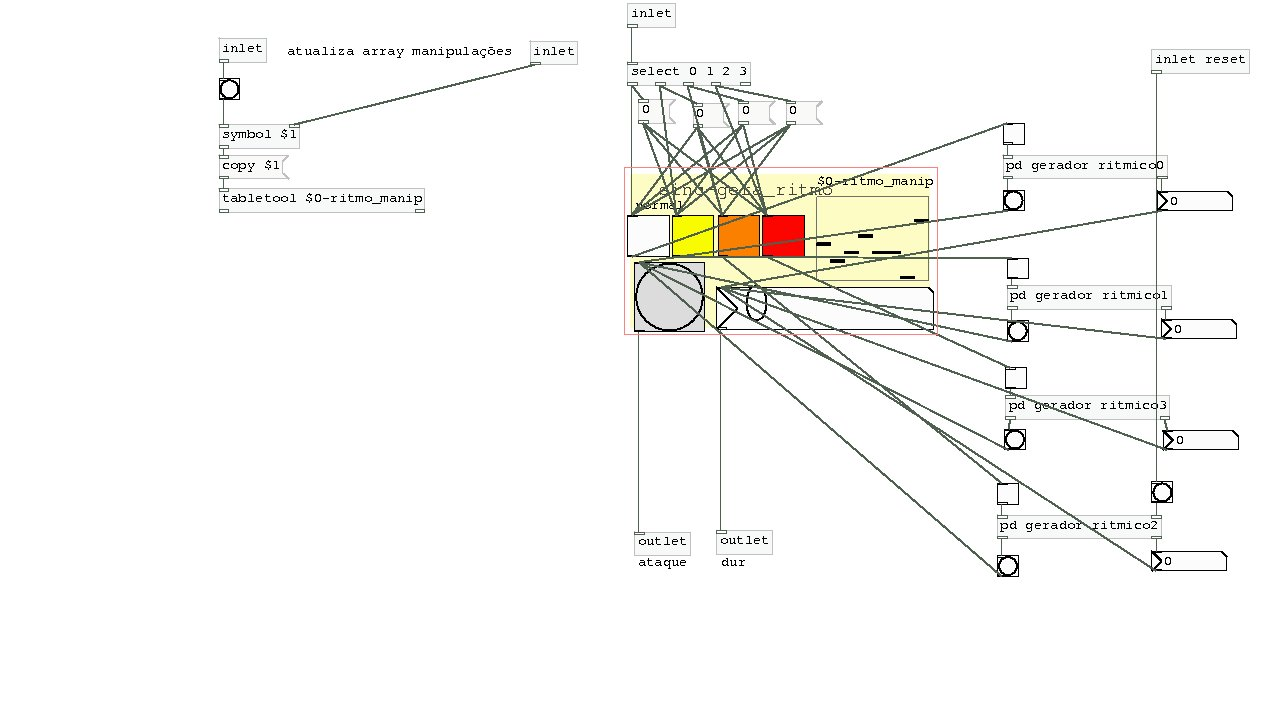
\includegraphics[scale=.5]{sinc-gera-ritmo}
% \caption{Objeto [sinc-gera-ritmico]}
% \label{[sinc-gera-ritmico]}
% \end{figure}
% 
% No atual estágio da pesquisa, foi implementada uma abstração gráfica
% que gerencia a atividade de quatro geradores rítmicos. Dessa
% maneira se torna fácil de administrar durante uma performance
% e também se mantém a flexibilidade de expandir para quantos
% geradores diferentes se queira. A interface pode ser vista na figura \ref{[sinc-gera-ritmico]}
% 

% sinc-gera-melodico 
% Da mesma maneira que os geradores rítmicos.....
% No atual estágio da pesquisa, foi implementada uma abstração gráfica
% que gerencia a atividade de quatro geradores melódicos. Dessa
% maneira se torna fácil de administrar durante uma performance.
% E também se mantém a flexibilidade de expandir para quantos
% geradores diferentes se queira.
% 
% 
% De maneira geral, os geradores melódicos dependem dos geradores
% rítmicos. Os geradores rítmicos "pedem" nota por nota para o geradores
% melódicos
% 
% 
% \begin{figure}
% 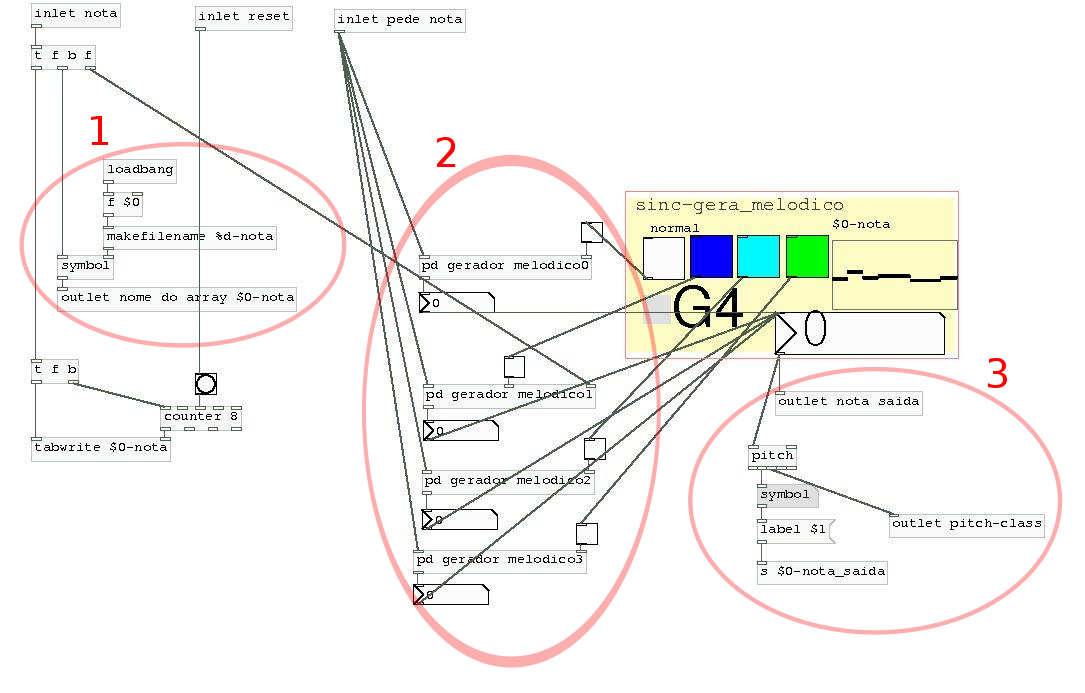
\includegraphics[scale=.45]{sinc-gera-melodico}
% \caption{Abstração que organiza 4 geradores melódicos}
% \label{[sinc-gera-melodico]}
% \end{figure}
% 
% \subsection{Geradores de amplitudes}
% 
% São encontrados diferentes termos definindo o aspecto
% da amplitude sonora como dinâmica (quando nos referimos a notação tradicional),
% velocity (quando se refere a dados MIDI), volume e amplitude (mais
% usado quando se refere a descrição física da onda sonora).
% 
% 
% As variações de amplitude podem produzir diferentes gestos musicais,
% Gerando acentos, diferentes articulações...



A manipulação de dados midi compreende algumas técnicas bem estabelecidas
no Pd. A geração de notas midi é realizada com o objeto [makenote] que formata
dados de entrada em notas midi, fornecendo as mensagens "noteon" e "noteoff", baseado
no valor de duração. As entradas e saídas midi são feitas com os objetos
[notein] e [noteout] respectivamente. O objeto [seq] grava e manipula arquivos 
do tipo midi, porém, os parâmetros das mensagens midi podem ser facilmente escritos
em arrays e listas para então serem manipulados.

\begin{figure}
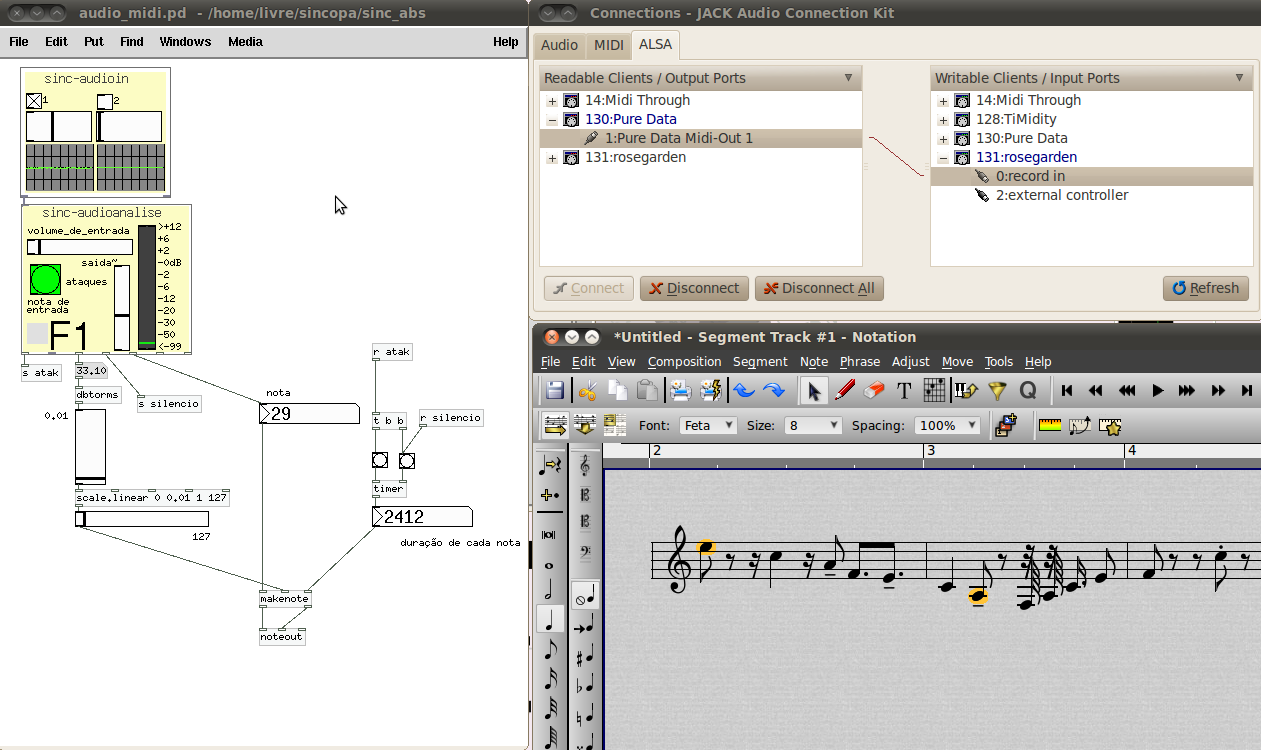
\includegraphics[scale=.37]{audio2midi}
\caption{Conversão de áudio para notas midi}
\label{audio2midi}
\end{figure}


Na figura \ref{audio2midi} vemos no patch a esquerda, o fluxo de entrada de áudio do objeto
[sinc-audioin], sendo analisado pelo objeto [sinc-audioanalise] e posteriormente
sendo convertido para mensagens midi com auxílio dos objetos [makenote] e [noteout].
Podemos observar ainda a dinâmica sendo convertida de decibéis (distribuição exponencial)
 para RMS (distribuição linear) com o objeto [dbtorms]. Após essa conversão,
o valor da dinâmica é convertido para uma escala midi de 0 a 127. Para isso é usado
o objeto [scale.linear] da biblioteca "pdmtl". O valor de duração das notas é determinado
pelo objeto [timer] que recebe uma mensagem (bang) a cada detecção de ataque e de silêncio.
No panorama geral da figura\ref{audio2midi} vemos o Pd mandando mensagens midi em tempo-real
para o programa Rosegarden, usando conexão midi do programa Jack. 



\subsection{Manipulação e escrita de dados MIDI}

% Explicar rapidamente como entram dados MIDI, como se estocam, analizam e explicar uma
% abstração simples que contenha esses elementos.
% 
% Objetivo da abstração: salvar o midi com a entrada e o gerador em um arquivo .midi

\begin{figure}
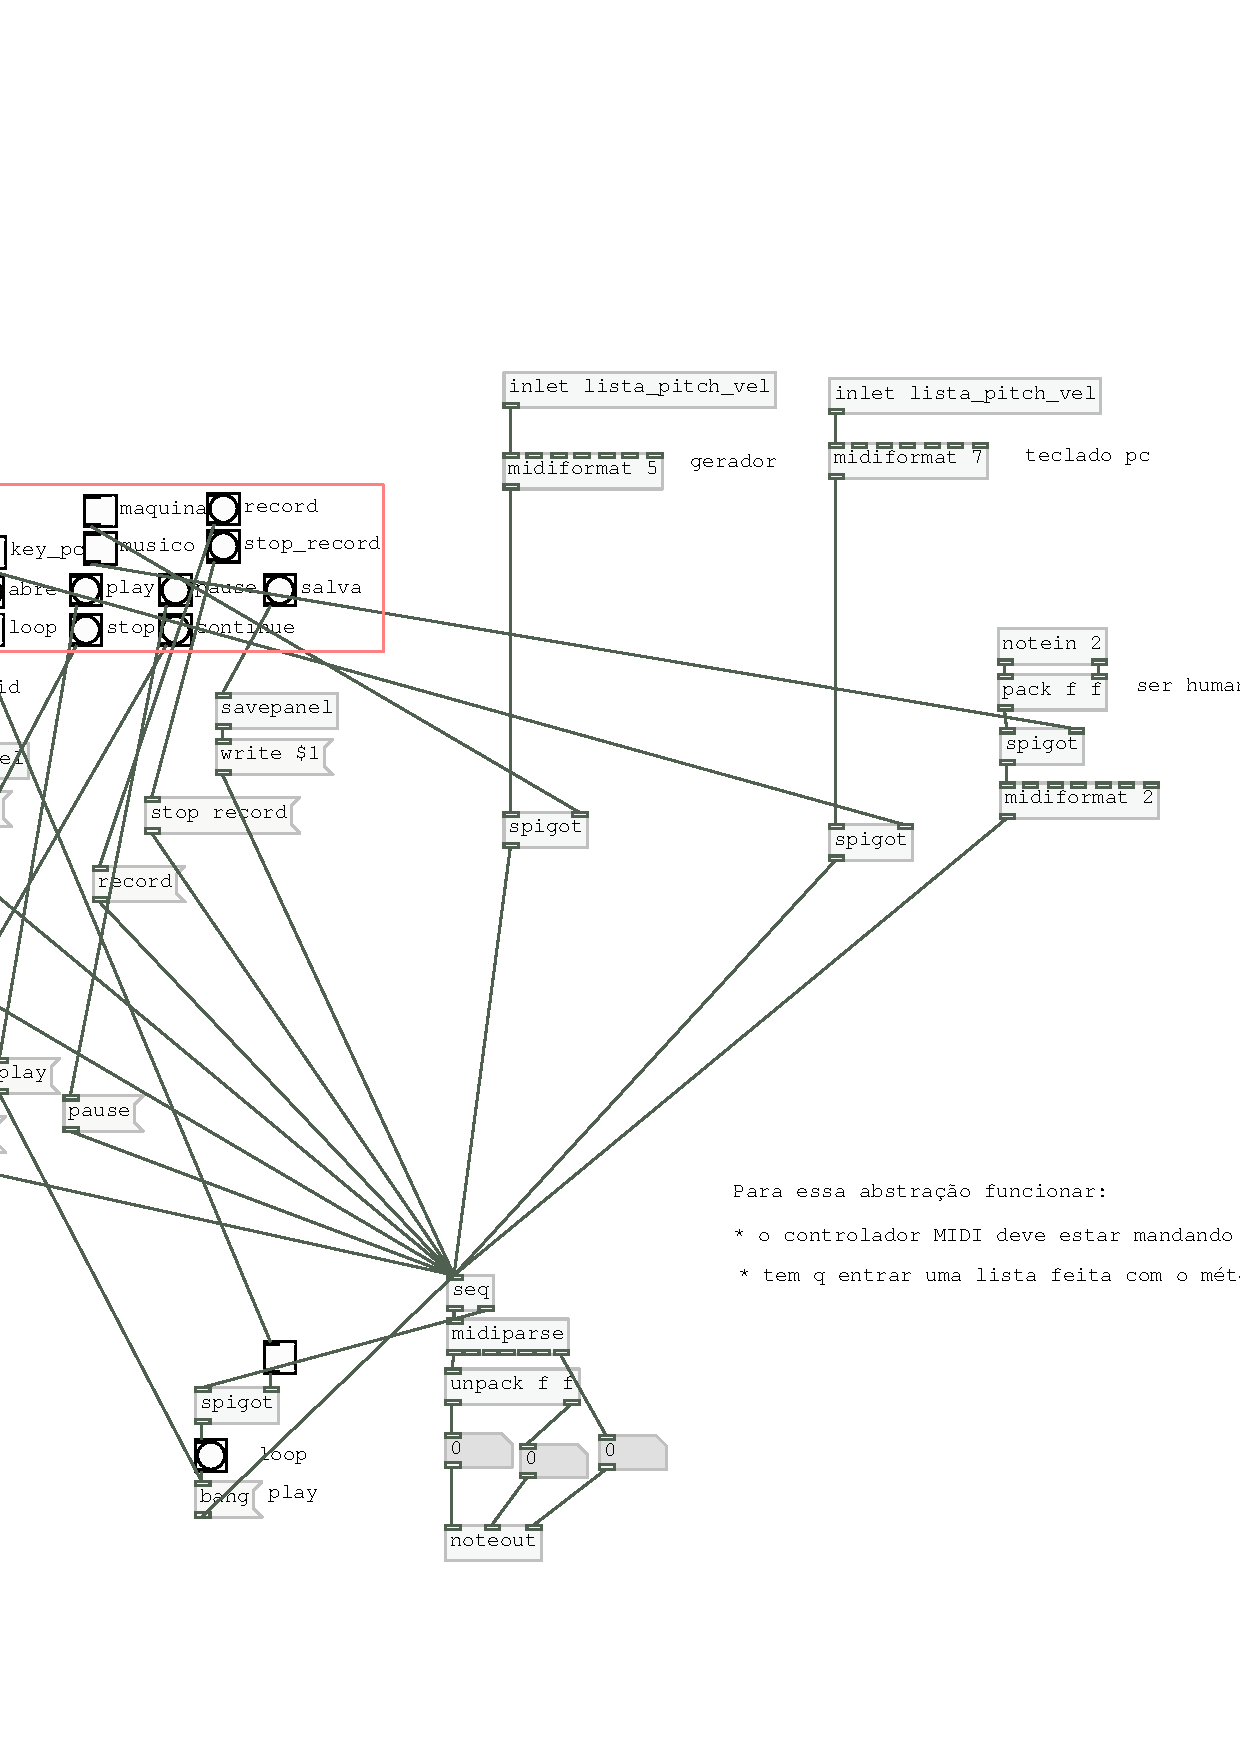
\includegraphics[scale=.5]{sinc-midiin}
\caption{Objeto [sinc-midiin]}
\label{sinc-midiin}
\end{figure}


\begin{figure}
\includegraphics[scale=.5]{sinc-midiin-help}
\caption{Exemplo de funcionamento de [sinc-midiin]}
\label{sinc-midiin-help}
\end{figure}



Existe uma discussão acerca da validade do protocolo MIDI na atualidade.
Caesar afirma que o protocolo MIDI enquanto ferramenta que se tornou um padrão
comercial, criou um ecossistema cultural e estético ao seu redor. Tendo influenciado
toda uma geração de compositores. Rowe por outro lado, coloca que a presença do
protocolo MIDI em sistemas musicais modernos é um anacronismo pois seria mais lento
que protocolos modernos como OSC\footnote{Open Sound Control} e incapaz de transmitir parâmetros mais completos
sobre a descrição musical, como por exemplo dados mais
refinados sobre o timbre. 

Apesar da discussão, o MIDI ainda é muito usado como padrão de troca de dados entre programas e 
como mapeador de instrumentos controladores comerciais. Além de ser usado em outros ambientes
como dispositivos de controle de iluminação e toques de celular. Apesar do título dessa seção
ser ``Geradores MIDI'', os algoritmos aqui apresentados podem facilmente ser utilizados como
geradores de síntese sonora ou usar outro protocolo de comunicação como o OSC.

O MIDI é um protocolo que descreve pitch (frequência), velocity (intensidade) e duração para cada
nota (evento). Isso permite que seja usado tanto em situações de gravação e repetição ou
transformação em tempo-real, quanto também como registro de uma sessão de interação.
Nesse caso, pode ser editado posteriormente em notação musical, como pode ser
visto na seção \ref{sec-notacao} onde podemos ver as possibilidades de integração
com outros programas para visualização da notação musical.

Foi desenvolvida uma abstração que facilita a leitura e escrita dos dados MIDI, baseada no
objeto [seq]. O objetivo é estabelecer uma metodologia para rápida prototipação, teste e registro
de algoritmos voltados para composição interativa.

A abstração recebe dados MIDI de controlador externo, dos módulos geradores algorítmicos e do
teclado do computador. Sendo capaz de gravar uma performance com dados de todas as fontes em
canais separados, o que garante uma posterior análise e re-utilização do material. Para isso
se definiu uma distribuição de canais MIDI como podemos ver na figura \ref{sinc-midiin}. Onde vemos
o objeto [notein] com argumento 2, que significa que apenas receberá dados enviados do canal MIDI 2.
Os objetos [midiformat] por sua vez aparecem com os argumentos 5 e 7, que garante a gravação
de um arquivo .mid com canais distintos.


Na figura \ref{sinc-midiin-help} vemos um exemplo de funcionamento recebendo dados do teclado do
computador com a abstração [sinc-teclado] ao mesmo tempo que recebe dados dos algoritmos geradores
melódicos. A abstração [sinc-gera\_melodico] controla os algoritmos de geração melódica e é acionada
por um [metro]. 


\subsubsection{Abstração [sinc-teclado]}


%% figuras :[sinc-teclado] interno + visão geral do mapa de [kbkey2] + figura que explica os argumentos de [kbkey2]

\begin{figure}
\includegraphics[scale=.5]{sinc-teclado-interno}
\caption{Visão interna de [sinc-teclado]}
\label{sinc-teclado-interno}
\end{figure}

\begin{figure}
\includegraphics[scale=.5]{sinc-teclado-mapa}
\caption{Mapa de distribuição das teclas de [sinc-teclado]}
\label{sinc-teclado-mapa}
\end{figure}

\begin{figure}
\includegraphics[scale=.5]{kbbey2}
\caption{Abstração [kbkey2] mapeia cada tecla}
\label{kbbey2}
\end{figure}

\begin{figure}
\includegraphics[scale=.5]{kbkey}
\caption{Abstração [kbkey]}
\label{kbkey}
\end{figure}


A abstração [sinc-teclado] foi feita como um acessório para rápida prototipação de 
performance com dados MIDI quando não se dispõe de um controlador externo. O objetivo
é transformar o teclado alfanumérico do computador em um controlador MIDI sem o controle de velocity
de cada nota. Cada tecla é mapeada com a abstração [kbkey2] o que permite que se defina como quiser
as relações de cada tecla com uma respectiva nota MIDI.

Na figura \ref{sinc-teclado-interno} podemos ver o panorama interno da abstração [sinc-teclado], onde podemos notar
que cada tecla envia uma mensagem MIDI por [noteout] para o canal 2.
Cada tecla é mapeada com a abstração [kbkey2] que é vista na figura \ref{kbbey2}. 
Na figura \ref{sinc-teclado-mapa} vemos a distribuição das instâncias de [kbkey2] para
cada tecla. Na figura \ref{kbbey2} vemos o detalhamento dos argumentos de criação de [kbkey2], que além de mapear
uma tecla específica para uma nota midi correspondente, envia informação para um objeto toogle [tgl],
correspondente a sua representação no teclado gráfico, o que possibilita a visualização para qual nota
a tecla foi mapeada. O primeiro objeto de [kbkey2] é a abstração [kbkey] que pode ser vista na figura \ref{kbkey}.




\subsection{Imitação}

Os geradores imitativos são os de implementação mais
simples, pois apenas fazem uma leitura na memória dos dados
da performance.
Quando algum parâmetro está sendo gerado através de imitação
a sensação de unidade composicional é fortalecida.



\subsubsection{Gerador rítmico imitativo}



\begin{figure}
\includegraphics[scale=.6]{gerador-ritmico0}
\caption{subpatch [pd gerador-ritmico0] de [sinc-gera-ritmico]}
\label{gera-ritmico0}
\end{figure}   


No patch da figura \ref{gera-ritmico0} vemos um gerador de tempos
de intervalo entre ataques de notas. Nesse caso, as durações dos intervalos
são gravadas no array \$0-ritmo\_manip. Aqui o array é lido com
[counter] que é acionado por um [delay]. O tempo de leitura respeita
o próprio valor de duração que é enviado com a variável [s tag].
A abstração tem duas saídas, a primeira envia um bang a cada nova 
leitura, e a segunda envia o valor da atual duração.

\subsubsection{Melodia imitativa}

Nesse primeiro gerador melódico o método de geração
é a leitura linear da tabela temporária de pitches
como se pode ver na figura \ref{gera-melodico0}.


\begin{figure}
\includegraphics[scale=.6]{gera-melodico0}
\caption{[pd gerador-melodico0]}
\label{gera-melodico0}
\end{figure}  

% \begin{figure}
% \includegraphics[scale=.55]{gera-mel0}
% \caption{exemplo de melodia imitativa gerada}
% \label{gera-mel0}
% \end{figure}  


%% esse exemplo gera-mel0.png é absurdo, tem muitos erros
%% preciso duma imagem
%% melhor..poucos compassos mas mais óbvio e bem acabado

O objetivo desse gerador é a imitação melódica
do instrumentista. A leitura é feita com [counter]
e enviada diretamente para a saída.





% \item

\subsection{Variação}
\label{varia-contorno}

%% aqui incluir operações de contorno
%% operações em arrays (transposição, inversão, retrógrado , rotação, normalização) - gerando midi

Denominamos variação um procedimento que toma como base um
material dado e aplica uma operação de transformação nesse material.
Nessa pesquisa, o material de base são os próprios dados da 
análise da performance musical.
Aqui serão descritos algumas técnicas de variação melódica como
transposição, inversão, retrogradação e também de variação rítmica
como expansão e contração de durações. Além de outras possibilidades
de leitura de arrays e transformações.

\begin{figure}
\includegraphics[scale=.6]{variacoes-contorno}
\caption{Patch mostrando operações de variação sobre array}
\label{variacoes-contorno}
\end{figure}  

Na figura \ref{variacoes-contorno} vemos acima um array ``pitch\_original'' que representa
o conjunto de pitches executados pelo músico (poderia ser durações ou qualquer
outro parâmetro). Abaixo, no centro, o array ``pitch\_resultado'' mostrando o resultado das  
operações de variação. E abaixo, um array ``contorno'' mostrando a redução do contorno em
``pitch\_original'' para a forma normal, como visto na seção \ref{contornos}.

\begin{figure}
\includegraphics[scale=.6]{variacao-normalizacao}
\caption{Sub-patch mostrando operação de normalização sobre array}
\label{variacoes-normalizacao}
\end{figure}  

A primeira operação é chamada aqui de normalização dinâmica, onde
se pode aumentar ou diminuir a razão entre os valores, sem perder
as relações originais. Isso é feito multiplicando todos valores por
um índice variável, como pode ser visto na figura \ref{variacoes-normalizacao},
onde vemos o subpatch [pd normalizacao]. A multiplicação é feita lendo
os valores em ``pitch\_original'' e escrevendo o resultado em ``pitch\_resultado'' e 
em outro array interno chamado ``temp''.



\begin{figure}
\includegraphics[scale=.6]{variacoes-interno}
\caption{Sub-patch [pd rj] mostrando objeto [c\_patternchange]}
\label{variacoes-interno}
\end{figure}  

As operações de transposição, inversão, retrógrado e retrógrado-invertido são 
realizadas com o objeto [c\_patternchange] da biblioteca rj. 
O objeto [c\_patternchange], recebe uma lista de valores na entrada
da direita e comandos de operações na entrada da esquerda. A cada novo
comando de operações, primeiro a lista atualizada de valores de ``temp'', 
com [tabdump], para então realizar a operação e escrever o resultado no
array ``pitch\_resultado''.

Paralelamente, é contado o tempo a cada chamada de operação com o objeto
[timer]. Quando o tempo entre uma operação e outra for maior que 500 milisegundos,
o objeto [tabletool] fará uma cópia de ``pitch\_resultado'' para ``temp''. O 
que garante que cada operação será feita em cima do resultado das outras operações
feitas durante a sessão. 

Quando aplicamos a operação de transposição ao parâmetro
de durações das notas, obtemos o efeito de expansão e contração
rítmica, bastante utilizados em técnicas de contraponto tonal.

\begin{figure}
\includegraphics[scale=.6]{gerador-ritmico1}
\caption{Gerador rítmico de variação de leitura de tabela de durações}
\label{gera-ritmico1}
\end{figure}  

Na figura \ref{gera-ritmico1} vemos outro gerador aplicado
a variações rítmicas.
É responsável por construir novas sequências rítmicas a partir de variações
da tabela de durações. Essas variações podem ser:
\begin{itemize}
 \item leitura das durações na ordem normal
 \item leitura na ordem reversa
 \item leitura randômica
\end{itemize}



% \item

\subsection{Randômicos}

%% imagem de patch mostrando resultados de print de random com notas na pauta


A maioria das linguagens de programação possuem um 
gerador de números randômicos, que gera a partir de uma distribuição uniforme, com valores entre 0 e 1. 
Esse número é chamado de pseudo-aleatório, porque é possível repetir a mesma sequência a partir de uma 
mesma semente (valor inteiro). A distribuição uniforme é a distribuição de probabilidades  
mais simples de definir, onde a probabilidade de se gerar qualquer ponto em um intervalo contido no 
espaço amostral é proporcional ao tamanho do intervalo.

Cada implementação define uma equação complexa que produz uma sequência de números
pseudo-previsíveis. No Pd o objeto [random] retorna um valor randômico entre 0 e seu argumento
de criação. O resultado pode ser escalado utilizando objetos matemáticos como visto na seção \ref{tecnicas}.
 

\begin{figure}
\includegraphics[scale=.7]{sinc-randplay}
\caption{Patch com dois geradores [random] alternando entre valores de seed}
\label{sinc-randplay}
\end{figure} 


\begin{figure}
\includegraphics[scale=.7]{rand-editar}
\caption{Sequência de notas geradas pelo patch da figura \ref{sinc-randplay}}
\label{rand-editar}
\end{figure} 

Cada instância de [random] é provida com uma semente (seed) que é apenas uma das variáveis na
equação que produz a sequência. A ``semente'' é gerada pelo Pd baseado em parâmetros específicos
em cada patch que contém um objeto [random]. Se mais de um objeto [random] é colocado em um único
patch, cada um recebe uma semente diferente. Entretanto, sementes podem ser enviadas para [random]
com a mensagem \textit{seed \$1}. Se mais de um objeto [random] recebem a mesma semente, ambos retornam
o mesmo resultado, e se a semente for atualizada com o mesmo valor, a mesma sequência 
de resultados volta ao início.

%% comentar as figuras

Na figura \ref{sinc-randplay} vemos um patch com dois objetos [random] acionados simultaneamente
pelo mesmo [metro]. Podemos notar que algumas mensagens com \textit{seed} aparecem acima. Algumas se conectam 
apenas com um [random] e outra se conecta com os dois. O resultado da manipulação desse patch pode ser 
visto na figura \ref{rand-editar} com a indicação acima da pauta do momento em que cada mensagem foi acionada.
Podemos dessa maneira sincronizar geradores randômicos e acessar repetições de trechos.


\begin{figure}
\includegraphics[scale=.6]{gera-melodico3}
\caption{[pd gerador-melodico3]}
\label{gera-melodico3}
\end{figure}  

Musicalmente podemos pensar num gerador randômico aplicado a geração de alturas, 
que representa o oposto da impermeabilidade melódica, como descrito por Ligeti e citado
no capítulo \ref{sec:rev}.
O gerador da figura \ref{gera-melodico3} é baseado no 
objeto [random.integer]. O objetivo desse gerador é 
ter um gerador com alto grau de permeabilidade melódica.

\begin{figure}
\includegraphics[scale=.6]{filtro-alturas}
\caption{Filtro de alturas baseado em array, através da abstração [musical.closest.note]}
\label{filtro-alturas}
\end{figure}  

Em alguns casos pode-se desejar realizar um filtragem
dos resultados de um gerador algorítmico. De maneira que
todos resultados do algoritmo se encaixe numa sequência
de valores definidos. Nesse sentido podemos citar a abstração
[musical.closest.note] da biblioteca PDMTL.

%% aqui falar de filtragem de alturas? 


%% aqui usar o [randomrange] - figura disso

\subsection{Probabilidades}

\begin{figure}
\includegraphics[scale=.6]{probabilidade-simples}
\caption{Patch controlador de probabilidade}
\label{prob-simples}
\end{figure}  

No Pd podemos implementar um sistema simples de probabilidade como 
vemos na figura \ref{prob-simples}, onde o resultado de um gerador
randômico passa por uma sequência de filtros numéricos feitos
com [moses]. Esse procedimento pode ser usado em conjunto com um sequenciador,
ou como é o caso aqui, pode ter as probabilidades ajustadas em tempo-real.

\begin{figure}
\includegraphics[scale=.6]{sinc-ritmo-prob}
\caption{Abstração [sinc-ritmo-prob]}
\label{sinc-ritmo-prob}
\end{figure}

Para criação de música interativa, é importante que as probabilidades
dos eventos de análise da entrada do músico, influenciem as probabilidades
de geração de eventos pelo sistema em tempo-real.
O objeto [probalizer] da biblioteca unauthorized, proporciona
uma interface gráfica para edição e controle das probabilidades.
Na abstração [sinc-ritmo-prob] foi implementada um sistema
que calcula as probabilidades de durações aproximadas.

Cada duração de entrada é encaixada em uma escala de cinco possíveis
classes de durações. De 0 a 200, 200 a 500, 500 a 1000 e 1000 a 1500 milisegundos
respectivamente, são os registros das durações das cinco classes,
da mais curta até a mais longa. 
Esses registros ainda podem ser móveis, alterando-se os objetos [moses]
através da entrada da direita.


A cada duração, é alimentado o objeto [probalizer], aumentando
a probabilidade da classe de duração em questão.
Quando [probalizer] recebe um bang através de [inlet pede-nota],
é retornado o valor da classe de duração de acordo com a curva
de probabilidade. Esse valor é enviado na variável [s indice-tempo]
para um gerador de durações. A cada classe que chega com [r indice-tempo],
um valor é calculado por um objeto [shuffle] correspondente. O objeto
[shuffle] retorna um valor randômico dentro de um registro dado. Por exemplo,
o primeiro objeto [shuffle] da sequência, vem com os argumentos 70 e 200, que determina
o registro do valor de resposta. 

\begin{figure}
\includegraphics[scale=.6]{gera-melodico1}
\caption{[pd gerador-melodico1]}
\label{gera-melodico1}
\end{figure}  

A cada 100 ocorrências de uma classe a tabela
de probabilidades volta ao início. Quando todos valores de [probalizer] estão
com a mesma probabilidade, o objeto funciona como um gerador randômico comum sem
repetições.
Outra aplicação de [probalizer] é vista na figura \ref{gera-melodico1},
onde cada valor de pitch da análise da performance do músico alimenta
a probabilidade da respectiva nota. O objeto [probalizer] é organizado
para receber valores de 0 a 127 e a cada 30 ocorrências do mesmo
pitch as probabilidades voltam ao início.


Uma outra possível aplicação seria a aplicação de probabilidades para
análise e geração de padrões maiores tanto de durações quanto de conjuntos
de notas. O que permite a recorrência dos padrões
rítmicos que emergem ao longo da performance.




\subsection{Movimento browniano}

%% ver rowe pg 306

\begin{figure}
\includegraphics[scale=.6]{gerador-ritmico2}
\caption{Gerador rítmico baseado em movimento browniano}
\label{gera-ritmico2}
\end{figure}  


O terceiro gerador é mostrado na figura \ref{gera-ritmico2} e
realiza uma combinação entre os objetos [tabletool] e [brown-rhythm].

O objeto [tabletool]\footnote{Objeto externo desenvolvido em C
por William Brent e compilado e testado no ambiente de desenvolvimento
dessa pesquisa} permite que se façam operações matemáticas
recursivas e análise em arrays de números. 

Nesse caso, [tabletool] é responsável por informar os valores
mínimo e máximo de durações de tempo entre notas, que estão
armazenados no array \textit{\$0-ritmo-manip}, enviando
esses respectivos valores como variáveis [s min-ritmo] e 
[s max-ritmo] para o gerador de durações [brow-rythm].


 \begin{figure}
\includegraphics[scale=.6]{brown-rythm}
\caption{brow-rythm}
\label{brown-rythm}
\end{figure}  

O objeto [brown-rhythm] está presente na biblioteca RTC e se trata de
um gerador de durações baseado em movimento browniano(\textit{Brown motion}
\footnote{movimento browniano é um modelo que descreve o movimento aleatório 
de partículas macroscópicas num fluido como consequência dos choques das 
moléculas das partículas. Esse nome é devido ao botânico Robert
Brown, que observou minúsculas partículas dentro dos vacúolos dos grãos de 
pólen executando um movimento agitado. Repetindo o experimento com partículas de poeira, 
ele foi capaz de definir que o movimento se deu devido às partículas estarem "vivas", 
embora a origem do movimento ainda estivesse para ser explicada.
O cientista que explicou corretamente esse movimento, propondo que a energia fosse 
constituída de partículas, foi Albert Einstein, em 1905.
Movimento browniano é um dos modelos mais usados de processos estocásticos
(ou probabilísticos) sobre tempo contínuo.} )

 \begin{figure}
\includegraphics[scale=.6]{brown-rhythm-func}
\caption{Funcionamento básico de [brow-rhythm]}
\label{brown-rythm-func}
\end{figure} 


O funcionamento básico aparece na figura \ref{brown-rythm-func}.
No manual de [brown-rhythm] aparece uma explicação mais detalhada.


\begin{quote}
Generates a brownian-movement-like rhythm of a geometrical row of
entry delays (ED) and a certain number of ED-values. The brownian factor
determines the distance between two succeding rhythmical values. A factor
of 0 produces a periodic rhythm, where a factor of 1 output random values 
of the given range.
\end{quote}  



Na figura \ref{brown-rythm} vemos como [brown-rythm] é construído internamente.
Nota-se em destaque os principais objetos envolvidos na construção
de [brown-rhythm]. Basicamente, o objeto [brownian] é uma implementação de
distribuição de Brown no Pd. E [trans-log] é um objeto que realiza uma
transição logarítmica entre números.

 \begin{figure}
\includegraphics[scale=.6]{brownian-func}
\caption{Funcionamento de [brownian]}
\label{brownian-func}
\end{figure} 

Podemos ver o funcionamento básico do objeto [brownian] acessando seu
manual (figura \ref{brownian-func}.  A saída desse objeto retorna números randômicos entre o mínimo
(''min'' (int, float)) e o máximo (''max" (int, float)). A distância entre
dois números randômicos é determinada pelo fator de brown (float
entre 0 e 1). Quando esse fator é 1, [brownian] se comporta como um
gerador randômico ordinário (objeto [random] por exemplo). Quando
o fator é 0, o mesmo número sempre é repetido.


\begin{figure}
\includegraphics[scale=.6]{brownian-exemplo}
\caption{objeto [brownian] com diferentes valores de fator de brown}
\label{brownian-exemplo}
\end{figure} 

É possível comparar diferentes comportamentos de [brownian] observando
a figura \ref{brownian-exemplo}, onde vemos três objetos [brownian] com
os mesmos parâmetros de inicialização, cada um escrevendo os resultados
em diferentes arrays de 50 elementos. A única diferença entre os 3 está 
no fator de brown, assinalado em rosa (0.01 , 0.1 e 0.5 respectivamente).
Musicalmente, um baixo fator de brown aplicado a durações entre notas
possibilita a emergência de padrões rítmicos bem estabelecidos com 
pequenas variações. Quando aumentamos gradualmente o fator de brown, ouvimos
uma transição rumo a uma instabilidade rítmica e a quebra de padrões. 
O objetivo desse gerador é se aproximar da performance do músico real.
O objeto [sinc-audioanalise] analise o áudio de entrada estimando os valores de duração entre notas.
Esse valores são enviados a [sinc-calc-ritmo] que faz uma estimativa do grau
de instabilidade, como explicado na página \ref{[sinc-calc-ritmo]} (como faz pra ref a página?).
O grau de instabilidade rítmica influencia direto o comportamento do fator de brown, de acordo
com a definição do cenário de interação a que se propõe. O cenário pode definir, por exemplo, que
um ritmo estável do músico (baixa instabilidade), provoque um comportamento rítmico instável
do gerador (fator de brown alto).



 \begin{figure}
\includegraphics[scale=.6]{brownian}
\caption{[brownian]}
\label{brownian}
\end{figure} 


Na figura \ref{brownian} vemos a composição interna do objeto [brownian] onde temos elementos
grifados com a cor verde e outros com a cor rosa. Se trata de duas partes
distintas do patch, a parte com a cor verde, representa o controle dos
parâmetros do objeto [drunk] que é a implementação de um modelo de \textit{random-walk}
no Pd. A área destacada em rosa mostra uma sequência de objetos que 
escalonam o resultado dentro da amplitude de valor mínimo (\$1) e máximo (\$2).

 \begin{figure}
\includegraphics[scale=.6]{drunk}
\caption{exemplo de funcionamento de [drunk]}
\label{drunk}
\end{figure} 

O objeto [drunk] pertence a biblioteca Cyclone, que tem como objetivo
implementar objetos compatíveis entre Pd e MAX. O objetivo de [drunk] é
retornar números randômicos dentro de uma escala variável. A distância
entre cada número randômico é definida pelo valor da terceira entrada
de [drunk]. Essa variável define o maior número de passos possível entre 
dois resultados de [drunk]. Podemos ver na figura \ref{drunk} que temos
dois objetos [drunk] sorteando 16 valores de 0 a 10 com a diferença do
número de passos, com 6 (destaque em verde) e 2 (destaque em rosa).

Os objetos [brownian] e [drunk] são muito úteis para a composição 
interativa por permitirem a variação dos parâmetros do algoritmo
em tempo-real. Essa funcionalidade é usada em SINCOPA em outros geradores
melódicos e de dinâmica.

\subsubsection{Movimento browniano como gerador melódico}


\begin{figure}
\includegraphics[scale=.6]{gera-melodico2}
\caption{[pd gerador-melodico2]}
\label{gera-melodico2}
\end{figure}  


O terceiro gerador é mostrado na figura \ref{gera-melodico2} e
realiza uma combinação entre os objetos [tabletool] e [brown-melody].




%  \item
\subsubsection{Gerador rítmico polifônico}


\begin{figure}
\includegraphics[scale=.6]{gerador-ritmico3}
\caption{Gerador rítmico randômico}
\label{gera-ritmico3}
\end{figure}  

O gerador da figura \ref{gera-ritmico3} é baseado no 
objeto [repchord-rhythm] da biblioteca RTC. O objetivo desse objeto é 
ter um gerador com capacidade de controle dos parâmetros da polifonia.

O objeto [repchord-rhythm] é um gerador rítmico polifônico cujas taxa repetição
e densidade do acorde são dependentes dos graus de periodicidade de durações
mínima e máxima entre notas. 
%\end{itemize}

\subsection{Boids}

Boids é o nome de batismo de um algoritmo simples, usado na simulação de deslocamento
de grupos de animais na natureza, como cardumes de peixe e bandos de pássaros.
Esse algoritmo foi inventado pelo animador de computação gráfica Craig Reynolds.
O nome é um trocadilho referindo-se a ``birds'' pronunciado com sotaque de Nova York.
Na definição, cada boid é um indivíduo pertencente a um coletivo.

Através da observação do deslocamento de bandos de pássaros, Reynolds conseguiu
descrever alguns padrões de deslocamento espacial dos indivíduos dentro do grupo.
É um modelo baseado no conceito de que cada indivíduo em um coletivo segue simples regras
comportamentais em relação aos seus vizinhos, e que a interação dessas regras
produz a propriedade emergente de um grupo coordenado.
Brevemente, as regras internas do algoritmo são:

\begin{enumerate}
 \item Os boids tentam voar em direção ao centro de massa dos outros boids vizinhos;
 \item Boids tentam manter uma pequena distância dos outros objetos (incluindo outros boids);
 \item Cada boid tenta sincronizar sua velocidade com boids vizinhos; 
\end{enumerate}

Basicamente, a cada instância temporal, os parâmetros espaciais de cada boid são re-calculados
levando em conta um centro de atração e os comportamentos dos vizinhos.
Esse algoritmo tem potencial enquanto gerador de material musical numa perspectiva de interação.

\begin{figure}
\includegraphics[scale=.6]{midi-boid}
\caption{Objeto [boids2d] controlando 3 boids geradores de notas MIDI}
\label{midi-boid}
\end{figure}  


O Pd-extended traz uma implementação de boids na forma do objeto [boids2d] que recebe mensagens de parâmetros
de comportamento global, parâmetros do centro de atração e calcula as novas posições XYZ de cada
boid. No caso de uma aplicação musical desse algoritmo foi pensado num primeiro momento que as frequências
podem representar o eixo X e o tempo de execução o eixo Y. 
Na figura \ref{midi-boid} vemos um array que representa a entrada de alturas do músico. Esse array atua como
o ``líder'' que é seguido por outros três boids. A altura e a velocity são enviadas para o objeto [boids2d],
que retorna o valor de altura e intensidade dos três boids que representam três vozes. Cada voz é escrita
em um canal MIDI.


\begin{figure}
\includegraphics[scale=.6]{boids-param}
\caption{Lista de parâmetros enviados para [boids2d]}
\label{boids-param}
\end{figure} 

As mensagens de parâmetros de comportamento global podem ser vistas na figura \ref{boids-param}. 
Cada parâmetro tem uma frase que explica a influência no comportamento global. Nesse experimento,
apenas o parâmetro \textit{attractpt} é atualizado em tempo-real, enquanto todos os outros são
fixos nos valores vistos em \ref{boids-param}.

\begin{figure}
\includegraphics[scale=.5]{boids-pianoroll}
\caption{Visão de resultado de 3 boids seguindo perfil melódico no piano-roll}
\label{boids-pianoroll}
\end{figure} 

O resultado do patch visto na figura \ref{midi-boid} pode ser visto
na figura \ref{boids-pianoroll}. Onde vemos que as notas executadas pelo array estão destacadas
em cores, enquanto que as notas geradas pelos boids estão em cinza. Podemos notar um certo ``atraso''
 na ação de seguir o ``líder''. Esse atraso pode ser alterado através dos parâmetros, por exemplo
o parâmetro \textit{inertia} que controla essa ``disposição'' para mudar de velocidade e de direção
está muito baixo (valor 2 na fig. \ref{boids-param}), a medida que aumentamos esse valor iremos notar
os boids seguindo com mais rapidez o ``líder''.
O efeito musical é uma textura que varia de uma polifonia densa e aparentemente disconexa até uma 
heterofonia radical, a depender dos parâmetros de comportamento.


%%fazer imagens: boidzz + mensagens globais + partitura de uma resultado com 4 vozes?

Outra classe de algoritmos podem ser encontrados na biblioteca ``flatspace'', especializada
em geradores fractais que aceitam parâmetros de ``atratores'' baseados em modelos da teoria
do caos. São objetos passíveis da atualização dos parâmetros em tempo-real. 
% Segue abaixo uma lista dos objeto geradores fractais:
% 
% \begin{itemize}
%  \item attract1 
%   \item base 
%    \item base3 
%    \item gingerbreadman 
% \item henon 
% \item hopalong
% \item  ikeda 
% \item latoocarfian 
% \item latoomutalpha 
% \item latoomutbeta 
% \item latoomutgamma 
% \item lorenz 
% \item martin 
% \item popcorn 
% \item quadruptwo 
% \item rossler 
% \item standardmap
% \end{itemize}



%%fazer imagem comparando essas desgraças

\subsection{Harmonizadores}


Essa seção tem como objetivo apresentar possibilidades de harmonização automática em tempo-real.
Onde o sistema tendo o conhecimento da linha melódica criada instantaneamente pelo músico, consegue
harmonizar essa linha melódica.

Uma extensa bibliografia tem sido desenvolvida nos últimos 30 anos sobre o tema da harmonização automática.
Muitas empresas subsidiam a pesquisa nesse tema com o objetivo de produzir produtos comerciais que realizem
harmonização automática de maneira satisfatória para o usuário final. Esse processo vem acumulando patentes
de algoritmos de harmonização por parte de companhias fabricantes de teclados e desenvolvedoras de programas comerciais
de produção musical. Um exemplo é o programa ``Band-in-a-Box'' que realiza harmonizações de acordo com
a análise prévia de estilos. Nesse caso a harmonização não é feita em tempo-real e tem como finalidade
o exercício musical caseiro de criação melódica sobre harmonizações de diferentes estilos.
Outro exemplo são as harmonizações automáticas de teclados comerciais populares, onde o usuário escolhe
a tonalidade manualmente e um programa interno realiza uma harmonização tonal, simples, mas muitas vezes 
satisfatória para certos estilos de música.

%% colocar na bibliografia os pdf's em ~/cristiano-doutorado/mat_tese/biblio_harmoniza

Ching-Hua Chuan define em sua tese, um sistema de harmonização que leva em conta parâmetros
de análise de cada nota presente em um fluxo melódico, como duração, duração das notas anteriores, número
de ocorrências de determinado pitch class ao longo da melodia, direcionalide melódica e diversos outros
parâmetros. Por fim, expõe um modelo de acompanhamento harmônico e obtém um resultado positivo ao apresentar
o sistema acompanhando canções populares.

Matt Hanlon e Tim Ledlie apresentam um sistema de harmonização de corais a quatro vozes no estilo de Bach.
A composição da progressão harmônica é implementada com um modelo estatístico de cadeias de Markov
(Hidden Markov Model), e deriva na solução da harmonia através da solução de problemas
de satisfação restrita (constraint satisfaction problem).Após
essa etapa é feita a realização da progressão em linhas melódicas para quatro vozes

Uma implementação bem detalhada de um harmonizador automático que faz uso de
 regras de harmonia tradicional é descrita na patente Norte-Americana 
US 7,189,914 B2  assinada por Allan John Mack. O harmonizador inicia
na primeira nota da melodia e de acordo com a escala e modo providos
pelo usuário, o sistema escolhe uma especificação de acorde dentre
as especificações estocadas em memória, que podem ser definidas pelo usuário
e são estocadas em arrays lidos pelo programa em tempo-real.
Nessa implementação, uma série enorme de regras de sequência harmônica e 
condução de vozes são definidas baseadas em regras comuns a diversos cursos
de harmonia tradicional, como evitar 5ªs e 8ªs paralelas e progressões
``proibidas'' (I - ii - iii , por exemplo).

Um aspecto complexo das regras de harmonia tradicional é que as regras
de condução das vozes se misturam de forma iterativa com as regras de
progressão harmônica. Na descrição da patente, o autor exibe trechos do sistema em pseudo-código,
mostrando a maneira como a sequência harmônica influencia na condução vocal e vice-versa,
e o nível de detalhamento do projeto:

\begin{verbatim}

VI to V progression
if the preceding and current chords are at their root positions then
  if the preceding chord is of dominant root then
    if the preceding chord is a triad in a minor key or a seventh in a 
      major key then
      if the current chord is a submediant triad then
	if the preceding chord has no seventh and no fifth then rule 361 fails
	if the third of the current chord has no double then rule 386 fails
      end if
    end if
   else if the current chord is a dominant triad then
    if the previous chord is a submediant triad in a minor key then
      if the current chord has no fifth then rule 361 fails
      if the third of the previous chord has no double then rule 386 fails
    end if
  end if
end if
\end{verbatim}

Dentro do escopo de SInCoPA, foram desenvolvidos alguns métodos de harmonização
melódica para uso composicional.
Pode-se pensar em relações não-usuais de parâmetros
como amplitude e densidade rítmica como controladores de 
comportamento de harmonizadores. 
Um dos objetivos é a flexibilidade e modularidade da implementação
de harmonizadores que possibilite novas relações e ``regras'' de
interação do músico humano com a dimensão harmônica da
composição. 


\subsubsection{Nota pertence ao acorde}
\label{harm-notapertence}
%% antigo::

Nessa técnica foi definido que a maior exigência será que o acorde contenha a nota que está sendo
tocada pelo músico e harmonizada pelo computador. 
Para isso são expostas 2 possibilidades de harmonização automática, com resultados distintos.

No patch da figura \ref{harm1}  temos a célula básica do harmonizador diatônico 
 usado no protótipo. 
O objeto [receive fiddle] recebe o fluxo de notas e o objeto [decide], escolhe 
randomicamente quais notas vão ser harmonizadas, e manda sua decisão para o objeto 
[spigot] que funciona como uma chave seletora liberando ou não a nota para ser harmonizada. 
Após a nota ser liberada para o harmonizador, vai acontecer  a escolha de qual acorde será 
sobreposto a essa nota. Isso é feito pelo objeto [random 4] que escolhe randomicamente um 
número de 0 a 3, cada um representando uma operação a ser feita com a nota dada pela flauta 
(ver ainda na figura \ref{harm1} - ``tabela de resultados de [random 4]'').

\begin{figure}
\includegraphics[scale=.6]{harm1}
\caption{Decisão de qual nota a ser harmonizada}
\label{harm1}
\end{figure}

\begin{figure}
\includegraphics[scale=.6]{harm2}
\caption{sub-patch ``pd tonica''}
\label{harm2}
\end{figure}

\begin{figure}
\includegraphics[scale=.4]{harm3}
\caption{resultado da harmonização com modo 1}
\label{harm3}
\end{figure}


Na figura \ref{harm2} podemos ver o que acontece dentro do sub-patch [pd tônica], onde a nota sorteada 
será a tônica de uma tríade maior ou menor dependendo do resultado de [random 2]. A figura \ref{harm3} 
mostra um pequeno exemplo dos resultados desse harmonizador. Nesse exemplo, a primeira nota 
harmonizada é um si que virou terça maior de uma tríade maior. Um aspecto interessante desse 
harmonizador é que mesmo em exemplos curtos quase sempre se chega a relações de mediantes 
cromáticas, como é o caso do terceiro e quarto acordes (Mib - Lab), nesse caso uma relação 
enarmônica de mediante cromática.

\begin{figure}
\includegraphics[scale=.5]{harm4}
\caption{harmonizador dissonante , modo 2}
\label{harm4}
\end{figure}

Apesar de muitas vezes os acordes gerados pelo harmonizador diatônico possuírem uma relação 
cromática, todos os acordes gerados são tríades maiores ou menores. Para criar um contraste 
foi criado um harmonizador de acordes alterados que está na figura \ref{harm4}. Nesse harmonizador todas notas 
que entram são tônicas e todas são harmonizadas. 
	A escolha do acorde para cada nota é feito através de distribuição de probabilidade, 
arranjado com o objeto [moses]. Quando uma nota entra, ela gera randomicamente um número de 0 
a 99 com o objeto [random 100], esse valor então é endereçado a um dos quatro tipos de tétrades 
possíveis nesse patch : aumentado com 7ª menor, alterado com 5ª diminuta (6ª aumentada Francês), 
menor com sétima maior ou maior com sétima maior. Cada uma das quatro tétrades tem 25 por cento 
de probabilidade de aparecer. Cada membro dos acordes é endereçado a um gerador de síntese aditiva 
com amplitude bem baixa. Em função da amplitude bem baixa do harmonizador de acordes alterados, o 
resultado funciona bem como uma textura dissonante .

% ainda falar dos modos 3 e 4 

%O presente trabalho é produto da fase inicial de investigação de minha pesquisa de doutorado. 

\begin{figure}
\includegraphics[scale=.4]{harm5}
\caption{pd, jack e rosegarden}
\label{harm5}
\end{figure}

O objetivo é a investigação de possibilidades e prototipação de estruturas computacionais com 
objetivo de agregar interatividade ao trabalho composicional.  
	Apesar desses harmonizadores terem sido usados nessa pesquisa para interação com áudio em 
tempo-real, podem ser muito úteis como geradores de material escrito em notação tradicional, 
como mostra a figura \ref{harm5}. Esta imagem mostra o patch de Pd mandando as informações para o programa 
de notação Rosegarden através do programa Jack que funciona como um servidor de comunicação entre 
programas.Esse tipo de operação possibilita uma usabilidade do Pd semelhante ao programa \textit{Open-music}\footnote{Disponível em:
http://repmus.ircam.fr/openmusic/home}
desenvolvido no Ircam.


\subsubsection{Acorde pertence a coleção de notas}



\begin{figure}
\includegraphics[scale=.6]{harm6}
\caption{Patch que harmoniza de acordo com as notas executadas pelo músico estocadas em um array}
\label{harm6}
\end{figure}

\begin{figure}
\includegraphics[scale=.6]{harm-colecao}
\caption{Resultado de harmonizador automático com acordes pertecentes a coleção de notas tocadas}
\label{harm-colecao}
\end{figure}

No patch da figura \ref{harm6} é implementado um harmonizador simples,onde a sequência dos acordes e
a condução vocal é totalmente randômica. A única regra é que as notas usadas na composição
dos acordes tenham sido tocadas pelo músico. Podemos ver o resultado desse algoritmo na figura \ref{harm-colecao}.

\subsubsection{Sequência baseada em regras}

% \begin{figure}
% \includegraphics[scale=.4]{harm6}
% \caption{Patch que harmoniza de acordo com as notas executadas pelo músico estocadas em um array}
% \label{harm6}
% \end{figure}
% fazer a imagem baseada em [sinc-chordseq]

\begin{figure}
\includegraphics[scale=.6]{sinc-chord}
\caption{abstração [sinc-chord] para criação de cada acorde }
\label{sinc-chord}
\end{figure}


Para implementação de regras mais refinadas de progressão harmônica foi desenvolvida uma
estrutura de decisão baseada em uma cadeia de markov. Para isso foi definida uma
estrutura de prototipação e definição de possíveis acordes de escolha pelos estados
da cadeia de markov.

A abstração [sinc-chord] vista na figura \ref{sinc-chord}, recebe uma variável global
``tonalidade'',  que varia de 0 a 127. Essa variável funciona como o elemento 0 na definição
do acorde. A definição do acorde é dada por quatro parâmetros definidos em cada instância
de [sinc-chord]. Por exemplo, se a variável ``tonalidade'' for definida como 60 (dó), uma instância 
definida como [sinc-chord 0 3 5 10] gera o acorde dó-mib-sol-sib (60 63 65 70).
A primeira saída é como mensagem MIDI, enviada a algum sintetizador externo, definida numa sequência
de objetos [poly], [pack 0 0 0] e [route 1 2 3 4]. Outra saída é uma lista com os quatro valores
de pitch do acorde, enviado por outlet para uso interno no Pd.


\begin{figure}
\includegraphics[scale=.7]{sinc-chord-list}
\caption{Abstração [sinc-chord-list] para listagem de diversos acordes}
\label{sinc-chord-list}
\end{figure}


A partir da definição de [sinc-chord], foi feito um protótipo de listagem de acordes
possíveis em [sinc-chord-list], visto na figura \ref{sinc-chord-list}. Na figura vemos
um objeto [select] principal que recebe a variável global ``novo\_acorde'' que aciona as instâncias
de cada tipo de acorde especificados pelo objeto [sinc-chord] correspondente.


\begin{figure}
\includegraphics[scale=.5]{harm-markov}
\caption{Exemplo de harmonizador baseado em cadeia de markov}
\label{harm-markov}
\end{figure}

A ordem de cada acorde na progressão é definido na figura \ref{harm-markov}.
A estrutura de decisão é baseada em uma cadeia de markov com três estados e 
nove possibilidades de resultado. Cada estado representa uma das três principais
funções tonais (tônica, sub-dominante e dominante). Dentro de cada estado foram definidas
algumas probabilidades de ocorrência de acordes. Por exemplo, se o acorde ``V'' 
for selecionado, a variável global ``state'' será enviada com o símbolo ``dominante'' e o próximo
acorde será com 70\% de chance ``vi'', 10\% ``IV'' e 20\% ``vii''. O resultado da escolha 
é enviada com a variável global ``novo\_acorde'' para [sinc-chord-list] para executar o
acorde escolhido.

O próximo passo da pesquisa em harmonização será criar um mecanismo que analise progressões
 e retorne as probabilidades de ocorrência que poderão mudar automaticamente as probabilidades
da cadeia de markov, alterando os valores dos objetos [moses], criando assim, novas relações
de probabilidade de progressão harmônica.

\pagebreak

\section{Geradores de Síntese}

As operações de síntese sonora são um campo em expansão para o
desenvolvimento de novos timbres. Em Pd podemos modelar
o timbre com operações matemáticas em sinal de
áudio a partir de geradores.
Na perspectiva de um compositor, programar em Pd abre um caminho
 para a livre experimentação e desenho
de áudio em tempo-real. A própria interface de
programação, exige que o músico/programador execute as 
conexões gráficas escutando os resultados das operações.
 A própria operação e vizualisação gráfica 
do resultado possibilita a precisão na concepção sonora do desenho
de áudio. 


O campo de pesquisa em síntese sonora digital é grande e vem crescendo
nos últimos anos. Com a possibilidade dos compositores atuarem ativamente
na concepção do timbre de suas composições, como é o caso dessa pesquisa. E
também pela emergência da atividade de desenho  de som\footnote{sound design}, 
principalmente no cinema, televisão e jogos. Dentro do campo do desenho
sonoro os principais focos de pesquisa são a captação e o áudio
processual\footnote{tradução livre de ``Procedural audio'' apresentado no artigo
 Designing Sound de Andy Farnell\cite{farnell2010designing}. Na tradução optei por
áudio processual, que reforça a idéia de criação de um ambiente sonoro interativo
em processo e se aproximar do sentido original:

\begin{quote}
 Procedural audio is sound qua process, as opposed to sound qua product. Behind this statement lies 
a veritable adventure into semiotics, mathematics, computer science, signal processing and music. 
Let us reformulate our definition in verbose but more precise modern terms before moving on. 
Procedural audio is non-linear, often synthetic sound, created in real time according to a set 
of programmatic rules and live input. To further define it let's explain it in terms of linear, 
recorded, interactive, adaptive, sequenced, synthetic, generative and AI audio. 
Let's also analyse some other phrases like algorithmic composition and stochastic music. 
By doing so, we may reach an understanding of why procedural audio is so powerful and important.
\end{quote} 
} que é um conceito amplo em que essa pesquisa pode estar inserida. 

Uma estratégia composicional a ser desenvolvida e devidamente
descrita é a consideração e demarcação de pontos de contraste total
entre som instrumental e som sintético. A partir dessa demarcação pode-se
explorar ``cenários de fusão'' e matizes sonoros fronteiriços entre
os pontos de contraste,. Alguns procedimentos semelhantes são usados
em técnicas de música espectral e música eletroacústica mista.
% , a diferença
% seria  e que possuam a capacidade de interagir dinâmicamente,
% evoluir no tempo de acordo com os estímulos do músico
% (faltou referência)

Nessa seção vão ser abordadas técnicas clássicas de síntese sonora
e maneiras de conectar essas técnicas com a análise
de áudio em tempo-real. O objetivo é criar situações
de diálogo entre instrumentos tradicionais e sons sintetizados.

Na implementação são usados objetos geradores de sinal como
por exemplo [osc\texttildelow] e [phasor\texttildelow] e
controladores de envelope sonoro como [line\texttildelow] e
[vline\texttildelow], além de escrita de áudio em arrays e 
mensagens de controle.
No Pd existe a necessidade de um cuidado na concatenação entre
sinais de áudio e mensagens de controle como visto na seção de metodologia \ref{tecnicas}.




Os resultados apresentados são na maioria implementações simples,
que são combinados durante a performance, oferecendo uma boa paleta
de sons reativos para o instrumentista/compositor. Para isso é
mostrada uma interface simples de todos módulos de síntese.
Ainda há muito a ser explorado no campo da síntese controlada
por parâmetros de análise de áudio, aqui é apresentado uma
metodologia de trabalho para expansão de possiblidades.






%% tá faltando muito revisar as referências





%%referencia:
% An introduction to procedural audio and its application in computer games.
% 
% Andy Farnell
% 
% Date: 23 September 2007
% http://obiwannabe.co.uk/html/papers/proc-audio/proc-audio.html



\subsection{ Objeto [sinc-gera-sintese]}


\begin{figure}
\includegraphics[scale=.6]{sinc-gera-sintese}
\caption{[sinc-gera-sintese]}
\label{sincgerasintese}
\end{figure}



Nessa abstração procura-se administrar a interação do músico
com diversas geradores baseados em diferentes técnicas de síntese,
oferecendo uma paleta de timbres ao compositor.

Os primeiros quatro sintetizadores descritos aqui, foram pensados como o mesmo
sintetizador, tendo sido implementados como quatro separados, como estratégia
composicional na organização das mensagens dos cenários de interação.




A superposição ou justaposição de diferentes sintetizadores vai
ser definida pelo comportamento pré-estabelecido pelo cenário de interação
proposto.





\subsubsection{Síntese aditiva com as notas da entrada de áudio}



\begin{figure}
\includegraphics[scale=.6]{gerador-sintese0-diato}
\caption{[pd gerador0-diato]}
\label{gerador0diato}
\end{figure}

Na figura \ref{gerador0diato} vemos um gerador de síntese
aditiva com três osciladores [osc\texttildelow] somados com
2 objetos de soma de áudio [+\texttildelow].

A frequência de cada oscilador é determinada por uma leitura randômica da
tabela de notas que são executadas pelo músico. Cada nota detectada pelo
objeto [sinc-audioanalise] é enviada para o array \$0-nota que tem 8 elementos.
Cada oscilador acessa esse array com o objeto [random] e manda a nota para o
objeto [mtof] que converte o valor de nota midi para valor de frequência.
Apesar das notas terem sido executadas pelo músico, as novas combinações 
de notas causadas pela leitura randômica cria uma sensação de elemento novo
no discurso musical.


Cada nota é acionada pelo objeto [metro] que tem argumento de tempo constantemente
re-calculado de forma randômica. O objeto [metro] produz pulsos regulares (bangs) de
acordo com o argumento que representa o valor de tempo entre cada bang em milisegundos.
Isso causa um ritmo fragmentado, gerando padrões rítmicos instáveis.

A amplitude desse sintetizador é fixa, com envelope feito com o
objeto [line\texttildelow]. As fases de ataque e decaimento de cada acorde 
são feitas com 2 mensagens, a primeira enviada imediatamente realiza o ataque 
e a segunda é agendada como o objeto [del] que realiza uma linha de atraso
responsável pelo decaimento . A amplitude resultante dos 3 osciladores é normalizada
com o objeto [*\texttildelow] com argumento 0.2.

No resultado da síntese é aplicado um delay com valor de escrita e leitura fixos.
O delay é obtido com a combinação dos objetos [delwrite\texttildelow] e 
[delread\texttildelow]. O áudio resultante da síntese é escrito em uma memória 
temporária com o objeto [delwrite\texttildelow] designado com o nome "delay3"
e tendo o tamanho total de escrita de 2000 milisegundos. Essa linha de delay
chamada "delay3" é lida pelo objeto [delread\texttildelow] e enviada
novamente para a escrita do delay com [delwrite\texttildelow], causando um
efeito de feedback de delay. Antes da leitura do delay ser enviado novamente
para a escrita, ele é normalizado com o objeto [*\texttildelow] em 0.7, o
que causa um efeito de eco ou reverb exagerado. 

O efeito musical resultante desse sintetizador é como se fosse um harmonizador que ecoa combinações inusitadas
das frequências executadas. O reconhecimento das frequências contrasta com o
ritmo randômico gerando uma familiaridade estranha.



\subsubsection{Síntese aditiva com frequências randômicas}

\begin{figure}
\includegraphics[scale=.6]{gerador-sintese0-rand}
\caption{[pd gerador0-rand]}
\label{gerador0rand}
\end{figure}


Esse gerador é basicamente igual ao anterior com a diferença de que
as frequências são totalmente randômicas, sem usar nenhum material
fornecido pelo músico. A escolha das frequências é feita baseada em um
objeto [random] com argumento 127, podendo aparecer qualquer valor de 0 a 127.
Os outros dois osciladores recebem esse valor randômico e cada um soma a esse,
outro valor randômico de 0 a 12, resultando em um acorde sempre com as três
notas dentro da mesma oitava.

Esse módulo de síntese é usado como contraste em relação ao anterior.
Dentro de um discurso musical interativo é importante que existam elementos
que proponham e acrescentem elementos estranhos ao que o músico executa.

Pode-se, por exemplo, usar em tempo-real o índice de análise de permeabilidade 
melódica executada pelo músico para a partir de determinado valor desse índice
o programa alternar automaticamente entre esses dois diferentes sintetizadores.




\subsubsection{Tempo de delay randômico com frequências da tabela} 

\begin{figure}
\includegraphics[scale=.6]{gerador-sintese1-diato}
\caption{[pd gerador1-diato]}
\label{gerador1diato}
\end{figure}


Esse patch cria variação dos tempos de escrita e leitura de linhas de delay, o que causa o
aparecimento de padrões rítmicos mais complexos e instáveis.
O resultado é uma textura que varia de sons sustentados (com valor de feedback alto) até
sons curtos, sempre com as notas da tabela de frequências executadas pelo performer.
A visão geral do patch pode ser vista na figura \ref{gerador1diato}.


\subsubsection{Gerador de frequências randômicas com tempo de delay randômico}

\begin{figure}
\includegraphics[scale=.6]{gerador-sintese1-rand}
\caption{[pd gerador1-rand]}
\label{gerador1rand}
\end{figure}

Esse patch é praticamente igual ao anterior, com a diferença de que as frequências
são sempre randômicas como pode ser visto na figura \ref{gerador1rand}. Cria um bom contraste 
em relação a sonoridade do anterior mantendo a semelhança da síntese aditiva com as linhas de delay. 
Para o músico, as situações interativas em que a frequência é totalmente randômica sempre são mais
desafiadoras pois aí o papel do performer acaba sendo conectar a lógica narrativa em gestos que a
princípio não estavam ligados.


\subsubsection{Síntese FM responsiva}

\begin{figure}
\includegraphics[scale=.6]{gerador-sintese-fm}
\caption{[pd fm1]}
\label{geradorfm}
\end{figure}


Na figura \ref{geradorfm} vemos um patch que realiza 
uma síntese por frequência modulada (FM). Todos os parâmetros
são conduzidos pela análise da performance musical.
Quando o sistema detecta uma pausa na execução, aciona um novo
sorteio de índice e frequência da moduladora.
A frequência da portadora é definida pela tabela de frequências
executadas pelo músico e a amplitude geral segue a amplitude
da performance.


\subsubsection{Ruído branco com filtro de frequências executadas pelo músico}

\begin{figure}
\includegraphics[scale=.6]{gerador-sintese-noise}
\caption{[pd noise]}
\label{geradornoise}
\end{figure}

O objetivo desse gerador é materializar a idéia de um
instrumento que esculpe um ruído branco ([noise\texttildelow]).
Nesse primeiro experimento da figura \ref{geradornoise}, foi usado 
um objeto [vcf\texttildelow], que é um filtro passa-banda controlado
por voltagem. O "voltagem" da definição do objeto se refere a analogia
do resultado sonoro com  o dispositivo de filtro controlado por voltagem
presente em sintetizadores analógicos. Se distingue dos outros objetos
de filtragem em Pd por usar uma sinal de áudio para definir a frequência
central. A cada detecção de pausa a intensidade do filtro é randomizada.



\subsubsection{Sintetizador com forma de onda variável}

\begin{figure}
\includegraphics[scale=.6]{gerador-sintese-waveform}
\caption{[pd synth-waveforms]}
\label{geradorwaveform}
\end{figure}


Nesse gerador, a cada detecção de pausa por parte do músico, o 
patch escolhe entre duas formas de onda para oscilar uma frequência 
definida em um array preenchido pelo próprio músico. Na figura
\ref{geradorwaveform} vemos a estrutura do patch. O objetivo
é criar variações de diálogo entre músico e computador.



\subsubsection{Sintetizador baseado em análise e resíntese}

\begin{figure}
\includegraphics[scale=.6]{gerador-resintese}
\caption{[pd gerador-resintese]}
\label{geradorresintese}
\end{figure}

\begin{figure}
\includegraphics[scale=.7]{banco-osc}
\caption{banco de osciladores}
\label{bancoosc}
\end{figure}

\begin{figure}
\includegraphics[scale=.7]{osc-base}
\caption{[pd osc]}
\label{pdosc}
\end{figure}



Esse sintetizador é baseado na idéia de análise espectral do fluxo
de áudio e resíntese a partir dos dados extraídos dessa análise.

A análise é feita com o objeto [sigmund\texttildelow] pré-definido com
as saídas "peaks" e "tracks", que retornam listas de frequência, amplitude e 
fase para, nesse caso, um banco de doze osciladores para cada saída como pode 
ser visto na figura \ref{geradorresintese}.
Nas figuras \ref{bancoosc} e \ref{pdosc} são mostrados o banco de osciladores no subpatch
[pd banco de osciladores] e a formação de cada subpatch do banco contendo um objeto [osc/texttildelow]
cada. 


\begin{figure}
\includegraphics[scale=.5]{spectro}
\caption{Espectrograma do som original e do som resintetizado}
\label{spectro}
\end{figure}
 
O efeito obtido pode ser chamado de resíntese de baixa resolução. O objetivo
inicial era produzir um sintetizador que fosse muito sensível a pequenas
variações timbrísticas. Por exemplo, quando um violonista pinça a corda do violão
com diferentes ângulos da unha, são produzidas variações espectrais sutis que servem
bem ao controle de síntese. Na re-construção do som o principal característica desse
gerador é um timbre robótico muito sensível a variações de timbre no sinal de entrada.
Pode-ver na figura \ref{spectro} um espectrograma comparativo entre uma amostra
de violão e a respectiva resíntese com esse gerador. Nota-se um certo "defeito"
de re-construção no trecho destacado, proveniente de uma variação timbrística provocado
por diferença do toque. 

% \begin{figure}
% \includegraphics[scale=.4]{prot2}
% \caption{protótipo 2}
% \label{prot2}
% \end{figure}



\pagebreak

\section{Processamento de sinal de áudio}


Algumas pesquisas demonstram interesse pela 
performance musical controlando parâmetros de processamento, como
em Grahan (colocar ref do rickygrahan.com)


%%performance conduzindo espacialização


Diversas técnicas de processamento digital fazem parte do repertório
composicional com computadores. Muitos programas de computador realizam
as mesmas técnicas com algumas diferenças na implementação.

As técnicas de processamento digital mais conhecidas emulam dispositivos
eletrônicos que operam no sinal analógico através de circuitos elétricos.
São muito comuns em estúdios a presença de "módulos de reverb" ou 
"pedais de efeito" para instrumentos. Na implementação computacional,
essas funcionalidades podem ser expandidas possibilitando controle em
tempo-real e integração com a performance musical, criando um ambiente
musical interativo que expande e transforma o gesto original do músico.

O principal objetivo dessa seção é criar ferramentas que re-combinem
o sinal de áudio de entrada de maneira a ser controlado pelo próprio
fluxo de áudio sub-sequente. Musicalmente são buscadas texturas que usem
o próprio áudio como fonte garantindo assim uma unidade sonora a partir da fonte.

Para aplicar uma técnica de processamento, primeiro se deve amostrar
o áudio a ser processado. No caso dos objetos de loop, o áudio é gravado
em um array e lido repetidamente nesse array. Já o delay variável vai ter uma
janela de escrita e de leitura variáveis desse sinal. O motor básico dos loops 
implementados são feitos com o objeto [tabplay\texttildelow] que lê arrays
de áudio sem alterar o tempo ou frequência. Esse objeto prevê um método de começo e fim
da leitura em número de samples.

\begin{figure}
\includegraphics[scale=.7]{sinc-ring}
\caption{Patch mostrando um ring modulator simples}
\label{sinc-ring}
\end{figure}


Também podemos processar o sinal de áudio em tempo-real, como é mostrado na 
figura \ref{sinc-ring} , onde é implementado um ring-modulator simples.


\begin{figure}
\includegraphics[scale=.55]{digitalia3}
\caption{Patch mostrando uso de objetos de SInCoPA misturados com objetos nativos e abstrações DIY2}
\label{digitalia3}
\end{figure}


Outros objetos e abstrações também são usados e comparados, durante as experimentações
como a biblioteca DIY2 e rj. Na figura \ref{digitalia3} podemos ver uma situação de prototipação
rápida, usando objetos de SInCoPA juntamente com objetos nativos de Pd e uma abstração DIY2 [mono-vibrato],
que implementa um ring modulator mais complexo. O patch mostrado na figura \ref{digitalia3} foi usado na
performance \textit{/usr/maquina4/compartida\texttildelow} com outros 3 músicos.

Uma parcela importante de técnicas de processamento de áudio digital corresponde as técnicas
de fusão espectral como phase vocoder, convolução e síntese cruzada. Vários autores vem trabalhando
para otimização desses efeitos em tempo-real\cite{porres},\cite{pd-tutorial}. 


\subsection{Delay variável}


\begin{figure}
\includegraphics[scale=.6]{sinc-delay}
\caption{Abstração de controle de delay variável}
\label{sinc-delay}
\end{figure}


O delay é um efeito que cria uma linha de atraso de áudio e possibilita
um leque grande de gestos sonoros.

Num módulo  de delay analógico, o músico escolhe diferentes elementos
da execução para aplicar delay de tempo variável: uma nota, um acorde 
da guitarra ou uma palavra do cantor. Essas decisões de certa forma 
sublinham esses elementos colocando marcas na audição. Essa chamada de
atenção para esses elementos acabam criando uma sensação de narrativa musical
interessante do ponto de vista composicional.

Foi criada uma abstração que possibilita uma linha de delay simples com valores
de tempo e feedback variáveis. A estrutura básica está na figura \ref{sinc-delay}. O objeto 
[delwrite\texttildelow] escreve uma linha de atraso de áudio de 500 milisegundos
num buffer de memória temporária com a variável \$0-delay. Essa linha é executada
pelo objeto [vd\texttildelow] colocando nele o argumento \$0-delay. Para se criar
o efeito de ``eco'' ou feedback, podemos enviar o áudio para ser somado com o sinal
original e enviado para [delwrite\texttildelow] novamente, criando assim, uma retro-alimentação
contínua de áudio. Para se determinar a quantidade de feedback podemos controlar a 
amplificação do sinal resultante antes de retornar a [delwrite\texttildelow].


Uma possibilidade de implementação mais refinada de delay é a técnica de ``delay espectral'' \cite{guidefft}, 
onde além da linha de atraso e feedback, pode-se controlar elementos
do timbre, uma vez que o sinal é decomposto por análise FFT e recriado a partir de
seus componentes de frequência, amplitude e fases separados.

\subsection{Repetição}


A repetição e contraste podem ser consideradas as duas principais forças
da composição. Nessa abstração buscou-se criar uma ferramenta que forneça ao músico 
a possibilidade de criar múltiplas linhas de repetição de tamanhos diferentes não pré-definidos.
O loop, ou repetição de um trecho de áudio é um procedimento comum,
sendo encontrado em diversos dispositivos e equipamentos de produção musical.


O mecanismo do loop baseia-se na escrita de linhas de áudio em arrays e subsequente
repetição. O músico controla a interface através de um teclado USB modificado e 
usado como pedal, explicado mais a fundo na seção sobre cenário de interação.

Nesse caso particular o objetivo é determinar outras construções rítmicas,
fora de controles MIDI e sequenciadores baseados em objetos [metro], ainda que essa opção
esteja sinalizada na implementação. A repetição
é baseada no tamanho da prórpia linha de áudio gravada.


\subsubsection{Objeto [sinc-loop]}


Em uma primeira implementação  vista na figura \ref{sinc-looper}, foi pensado um loop simples. Com um botão
que seleciona o canal, outro botão que quando pressionado começa 
a gravar e quando pressionado novamente pára a gravação e automaticamente
começa a repetir o trecho gravado. A implementação é baseada no objeto
[timer] para medir o tempo entre o começo e o final da gravação. O objeto
[tabwrite\texttildelow] opera a gravação em um array e o objeto [tabplay\texttildelow]
executa o áudio gravado.

Na figura \ref{loopmaster}, vemos a implementação de [sinc-loop-master], que leva a frente
o mesmo mecanismo acrescentando um metrônomo e um contador global. A função desse contador
é uma possível futura sincronia com sequenciadores diversos, inclusive para performance
musical via rede (música telemática). Para a execução do loop pode ser levado em conta
o metro global ou não. A divisão entre cores facilita o estudo do fluxo dos dados.
A abstração [sinc-loop-slave] é uma versão sem o contador global e pode ser vista
na figura \ref{loopslave}. O uso concatenado é visto na figura \ref{loophelp}, onde vemos
a presença de um [sinc-loop-master] e três [sinc-loop-slave].


 Existem diversas situações de loop comuns na produção musical mediada por tecnologias digitais
como por exemplo, linhas de loop com tempo livre como nos pedais de efeitos, onde o instrumentista
tem um certo número de linhas de audio disponíveis e alguns botões de controle.
E situações em que a linha de áudio gravada em tempo-real pelo músico é esticada ou encolhida o mínimo
possível para encaixar na métrica de um sequenciador como por exemplo o sequenciador
comercial Ableton live. Não cabe aqui julgar o valor estético causado por uma ferramenta. Mas sim
trazer à tona a discussão sobre a consciência, por parte do compositor, da natureza da ferramenta 
e de como o pensamento composicional interage com essa interface.


Para a continuação dessa pesquisa o ideal seria um sistema de loop baseado no objeto 
[tabread4\texttildelow] que permite o "stretch" da leitura do áudio. Isso possibilita que o programa
ajuste o loop a qualquer tempo pré-definido por algum sequenciador.

\begin{figure}
\includegraphics[scale=.5]{sinc-looper}
\caption{loop simples}
\label{sinc-looper}
\end{figure}




\begin{figure}
\includegraphics[scale=.4]{loop-master}
\caption{[sinc-loop-master}
\label{loopmaster}
\end{figure}


\begin{figure}
\includegraphics[scale=.2]{loop-slave}
\caption{[sinc-loop-slave]}
\label{loopslave}
\end{figure}

\begin{figure}
\includegraphics[scale=.6]{loop-help}
\caption{Uso de dois [sinc-loop-slave] e [sinc-loop-master]}
\label{loophelp}
\end{figure}


\subsection {Fragmentação}


\begin{figure}
\includegraphics[scale=.6]{sinc-gravador}
\caption{[sinc-gravador]}
\label{sinc-gravador}
\end{figure}



A recombinação de trechos sonoros executados previamente é uma grande fonte
de gestos musicais e experimentação sonora. Um fluxo de áudio quando gravado
e fragmentado em trechos pode criar uma sensação de descontinuidade e não-linearidade
da memória curta ao mesmo tempo que guarda uma unidade perceptual em função de estar usando
o áudio que acabou de acontecer.

O objetivo desse módulo é fazer com que trechos do áudio da performance sejam segmentados e 
passíveis de recombinação em diversos modos e também controlados pela execução musical.

O primeiro elemento dessa abstração é um gravador de áudio que escreva um fluxo
de áudio em uma tabela (array) que possa ser acessado pelo motor de recombinação de "fatias" de áudio.
Uma pequena abstração com essa finalidade pode ser vista na figura \ref{sinc-gravador}.
%% descrever entradas e saídas de [sinc-gravador]

\begin{figure}
\includegraphics[scale=.6]{slicer3}
\caption{Fatiador automático de segmentos simétricos}
\label{slicer3}
\end{figure}

\begin{figure}
\includegraphics[scale=.6]{sinc-slicer}
\caption{[sinc-slicer}
\label{sinc-slicer}
\end{figure}

O funcionamento básico de um sistema de segmentação de amostras de áudio pode ser visto na figura \ref{slicer3},
baseado nos objetos [vline\texttildelow] e [tabread4\texttildelow]. Nesse caso os segmentos são feitos
automaticamente baseados na duração total da amostra e feitos de maneira simétrica.
O motor central da execução dos segmentos é mostrado no detalhe da figura \ref{slice-motor}.
A relação está no fato do objeto [vline\texttildelow] cria uma linha de leitura que é interpretada
por [tabread4\texttildelow] como valor de início e fim de leitura em samples e tempo dessa
leitura o que acaba por afetar a duração ea frequência do áudio resultante. 
A abstração [sinc-slicer], é uma interface mais refinada e pode ser vista na imagem \ref{sinc-slicer}, 
onde os pontos de início e fim do segmento são definidos pelos dois sliders abaixo da forma de onda.

\begin{figure}
\includegraphics[scale=.6]{slice-motor}
\caption{Motor básico da segmentação do áudio}
\label{slice-motor}
\end{figure}

Durante o andamento da pesquisa, foi usada a interface do projeto Navalha de Guilherme Soares,
como princípio de experimentação.
O Navalha é uma ferramenta que estabelece
um método para segmentação e sequenciamento de recortes de amostras de áudio. A interface gráfica
provê acesso as funcionalidades, como carregar sample, segmentar trechos manualmente, sequenciar e 
salvar presets. Ao mesmo tempo é possível usar o Navalha sem a interface gráfica, embutido em outro
projeto como é o caso aqui nessa pesquisa.

A funcionalidade da interface é bem completa e permite acesso a muitos aspectos da segmentação e do
sequenciamento.

\begin{quote}
 O objeto nvl cria instâncias de um sequenciador de fatias (slices) de .wav que podem ser editadas e salvas na 
própria interface gráfica deste objeto.
Estabelece também um arquivo padrão de metadados que permite que estas fatias sejam recarregadas na 
exata posição de onde foram salvas anteriormente – o arquivo .nvl.

Estas fatias podem ser tocadas de maneira não-linear modificando padrões (patterns) de um sequenciador 
embutido que toca numa velocidade determinada em batidas por minuto (podem ser subdivididas dentro desta 
mesma batida) a atual fatia numa sequencia determinada por este “pattern”.

Os objetos [nvl] podem ser conectados em cascata, pelos seus primeiros inlets e outlets – determindo 
assim um master da conexão mais acima que pode sincronizar os sequenciadores de patterns – determinando um 
“master sequencer” que irá controlar os demais “slaves” nvl.
Estes pattern também podem ser salvos dentro do arquivo .nvl criando assim uma possível navegação de clichês 
(ou “riffs”) que podem ser recuperados e repetidos durante uma performance.

Os controles de edição da performance já estão todos mapeados para controlesvia teclado do seu computador. 
Se você necessita desligar esta função num objeto nvl, basta desligar a função “key” que fica no canto inferior 
esquerdo. Obviamente se duas instâncias nvl estiverem com “key” ligado, ambas serão controladas simultaneamente 
pelo seu teclado. \cite{navalha}
\end{quote} 

\begin{figure}
\includegraphics[scale=.6]{nvl1}
\caption{Visão geral das entradas e saídas do objeto [nvl]}
\label{nvl1}
\end{figure}

\begin{figure}
\includegraphics[scale=.6]{nvl2}
\caption{Detalhe dos controles do sequenciador do [nvl]}
\label{nvl2}
\end{figure}


Podemos ver na figura \ref{nvl1} uma visão geral das entradas e saídas do objeto [nvl] e na figura
\ref{nvl2} um detalhamento dos controles do sequenciador embutido que são explicados na lista abaixo.

\begin{quote}
\begin{description}
  
\item a) Outlet de saída do sincronismo master-slave. Conduz o cursor do sequencer e o bpm atual.
\item b) Outlet que mostra a posição atual do cursor.
\item c) Sequencia de slices que será executada durante a passagem do cursor master.
\item d) Selecione a simetria de fatias desejada.
\item e) Escolhe um número limite de slices que será randomizado e cria uma sequência de números randômicos para um pattern.
\item f) Pattern de uma sequencia padrão para frente e para trás e zero.
\item g) Carrega 10 patterns diferentes que estão salvos na matriz buffer da memoria. Estes patterns são carregados no arquivo .nvl ou podem ser salvos com o procedimento descrito abaixo no item “h”.
\item h) Botão store (ou atalho shift+s) serve para atualizar no buffer de memória ram (não salva em disco) os atuais presets dos slices e patterns. Para salvar em disco, voce precisa dar um nome de arquivo na janela save-preset do canto inferior direito.
\item i) Number box que define o número de células que o cursor vai correr. Isto torna possível fazer uma sequência com tempos ímpares ou diferentes de 8 batidas por compasso.
\item j) Liga/Desliga os atalhos do controle de teclado.
\item k) Liga/desliga sequencia master. É possível tocar mais de um master, mas obviamente não estarão imediatamente sincronizados.
\item j) Cursor do sequenciador, dispara fatia atual.
\cite{navalha}
\end{description}
\end{quote}

\begin{figure}
\includegraphics[scale=.6]{controls-nvl}
\caption{controle externo dos parâmetros do navalha}
\label{control-nvl}
\end{figure}

\begin{figure}
\includegraphics[scale=.6]{mininvl}
\caption{[mininvl]}
\label{mininvl}
\end{figure}

Na figura \ref{control-nvl} vemos as mensagens que permitem controles externos do navalha.

Ainda no tutorial:

\begin{enumerate}
\item slice (numero da fatia) 
\item tempo (com duas variaveis – bpm e divisao do compasso)
\item preset (nome do arquivo nvl – que deve estar na pasta presets)
\item pattern (numero do pattern do buffer de 1 a 10)
\item key (liga e desliga acesso a teclado)
\item seq (liga e desliga sequenciador)
\item vol (volume de 0 a 1)
\item random (numero limite da celula do pattern seguido de gerador randomico de pattern)
\item pitch (intervalo em semitons em relação a nota atual)
\item div (numero de celulas no compasso atual do sequenciador)
\item normalize (bang – normalizar a faixa na ampliude máxima)
\item mono2x (bang – duplicar uma faixa mono para dar um falso efeito estereo)
\item simetria (numero de slices – cria slices simetricos em divisao exata do tempo total)
\item wav (nomedoarquivo.wav abre um arquivo .wav que esteja na pasta samples)
\cite{navalha}
\end{enumerate}


Nesse projeto, o mapeamento do áudio do músico controla aspectos do sequenciador como o tempo,
o número de segmentos e acionamento individual de cada segmento. O funcionamento
pode ser visto numa interface minimalista do objeto [nvl] na figura \ref{mininvl}.
Muitas outras variações de controle podem
ser pensadas e definidas em diferentes cenários de interação.






% * fazer uma máquina que grave trechos e salve um wav na pasta do navalha
% 
% * mapeamento das notas do violão para controles do sequencer do navalha
% 
% * a estabilidade rítmica liga o sequencer com o metro imitando a tabela de durações
% 
% * quando estiver instável liga o mapeamento das notas com os slices
% 
% 
% * explicação do básico de como funciona com o patch do tim vets
% 
% 
% 
% 
% 
% * loop fatiado em tempo-real misturado com sequenciador 

%%http://www.timvets.net/software/pd-beatslicer.php?page=software

\subsection{Síntese granular}




\begin{figure}
\includegraphics[scale=.6]{granular2}
\caption{abstração [grainvoice]}
\label{granular2}
\end{figure}

\begin{figure}
\includegraphics[scale=.6]{granular3}
\caption{subpatch gerador de uma curva de Gaussian}
\label{granular3}
\end{figure}

Síntese granular é uma técnica que combina síntese aditiva e amostragem (sampleamento).
Cada "grão" é um trecho de uma amostra de áudio somado a outros grãos, podendo
resultar em texturas únicas, que seriam praticamente impossíveis de serem editadas
grão por grão em um editor de áudio. Os resultados variam desde um leve deslocamento na leitura
de uma amostra até efeitos mais complexos como "nuvens de grãos".

Dois efeitos familiares são time-stretching e pitch-shifting, que podem ser vistos
como dois lados de um processo em comum chamado pitch synchronous overlap an add (PSOLA).
Um som pode ser dividido em pequenos segmentos que se sobrepõe e então cada segmento
é executado em sequência de maneira que o som original seja obtido. Para extender um
som se adiciona cópias extras dos grãos mudando a extensão e a duração de sobreposição
de maneira que a extensão total seja maior ou menor que a original. Nesse caso todos os 
grãos são obtidos da mesma fonte sonora.

Foi desenvolvida uma abstração com objetivo de possibilitar síntese granular em tempo-real usando como
fonte sonora o próprio som do instrumento que está sendo executado. E além
disso facilitar o controle dos parâmetros da síntese granular pela análise
da performance do músico. Diversos efeitos e texturas complexas podem ser obtidas
através do gesto de controlar parâmetros dos grãos com um instrumento.

O motor de funcionamento da síntese granular é baseado em modificações de um exemplo
do livro "Designing Sound" \cite{farnell2010designing}. Podemos ver na figura \ref{granular2}, a estrutura
da abstração [grainvoice], que define o comportamento de uma "voz". Nesse contexto,
"voz" significa uma camada de grãos justapostos. O funcionamento básico se dá através
de um leitor de tabela ([tabread4\texttildelow source-array])que é modulado por um gerador de envelope ([tabread4~ grain-env]).
Os dois arays são visíveis na visão geral do patch na figura \ref{granular-geral}. O array grain-env
é definido no subpatch da figura \ref{granular3}, e se trata de uma janela "raised cosine", também
chamada de "hanning window" que é computada como 0.5+cos(x)/2 entre -pi e +pi.

O componente central de [grainvoice] é um objeto [vline\~], que recebe uma mensagem para criar uma linha que 
vai de 0.0 a 1.0 durante um certo intervalo de tempo. Esse intervalo de tempo é a duração
do grão, que é substituído no segundo elemento da segunda lista da mensagem de [vline\~].
A linha gerada aciona simultaneamente os dois arrays e posteriormente 
seus resultados são multiplicados.

Os parâmetros grainpitch, graindur e grainstart controlam o som resultante. Esses aparecem sob duas
formas. Primeiro, como variáveis globais e determinam a frequência, duração e ponto de início de leitura para
todos os geradores de grãos ([grainvoice]) do patch inteiro. As variáveis globais são modificadas
por versões locais (com prefixo \$0-my) que determinam parâmetros únicos para cada instância de [grainvoice].
Quanto maior a diferença entre os parâmetros de cada voz mais nos aproximamos do efeito de "nuvens de grãos".

\begin{figure}
\includegraphics[scale=.6]{granular-geral}
\caption{Visão geral de funcionamento de síntese granular}
\label{granular-geral}
\end{figure}


Na figura \ref{granular-geral} são usadas quatro instâncias de [grainvoice]. No canto inferior esquerdo da figura
vemos o controle das quatro variáveis globais. Observando que o objeto [soundfiler] envia o tamanho do arquivo
carregado, em número de amostras, através da variável filesize. O primeiro controle usa esse valor para escalonar
o parâmetro grainstart de maneira que o valor 0.0 sempre represente o começo do arquivo e 1.0 o final do mesmo.
A duração do grão é controlada por graindur e é dada em milisegundos, variando de 10 mseg até 2000 mseg.
A frequẽncia do grão é centrada em 1.0, que executa o arquivo no usual 44.1kHz. Ao mover o slider para a esquerda
ou direita do centro, ele retarda ou acelera a execução da amostra. Por último vemos o parâmetro overlap que varia de
1.0 a 2.0.

A parte principal do patch da figura \ref{granular-geral} está na direita. É um sequenciador baseado no objeto
[metro] controlando um contador que devolve números entre 0 e 3,que servem como índices de listas que ao final
são roteados com o objeto [route] para quatro instâncias da abstração [grainvoice]. Cada lista contém ainda dois
valores randômicos para cada instância de [grainvoice]. A frequência do objeto [metro] é calculada de acordo com a duração
do grão . Aqui é onde a variável
overlap também influencia. Se overlap tiver o valor 2, a frequência de [metro] será 1/4 da duração
do grão de maneira que a execução do primeiro grão irá finalizar em tempo de ser executado novamente.
Para valores menores haverão menos sobreposições (overlaps) de grãos. Essa variável muda a densidade da
textura, variando de um efeito de deslocamento da leitura da amostra que pode lembrar um efeito de 
"chorus" até variações mais caóticas. Por fim é acrescentada uma abstração de reverb ([rev3\~]) ao final
do áudio do patch.



\subsubsection{Objeto [sinc-granular]}



%% figura da visão geral da alteração de overlap

\begin{figure}
\includegraphics[scale=.7]{sinc-gran1}
\caption{visão geral da alteração de overlap}
\label{sinc-gran1}
\end{figure}

\begin{figure}
\includegraphics[scale=.6]{sub-randomize}
\caption{subpatch [pd randomize]}
\label{sub-randomize}
\end{figure}


Nesse módulo também foi usada a abstração [sinc-gravador] já vista na figura \ref{sinc-gravador}.
Com finalidade de facilitar a interação em tempo-real com um músico.

Outra parte da abstração, diz respeito ao mapeamento dos dados de análise para controle
dos prâmetros de síntese. Um elemento alterado em relação ao exemplo original de Andy
Farnell é a definição da variável local \$0-mydur, onde é acrescentado um subpatch que 
possibilita definir um valor fixo ou randômico para todas as vozes, resultando assim, numa variação entre
uma textura mais síncrona e outra mais assícrona. Como pode ser visto na figura \ref{sinc-gran1},
e no detalhe do subpatch na figura \ref{sub-randomize}.


\pagebreak

\section{Cenário de interação}


O conceito de cenário aqui é usado como a maneira de concatenação
entre os parâmetros da análise de áudio e os geradores de material
musical.


Cada parâmetro da análise da performance do músico pode ser mapeado como controlador
de algum aspecto da geração de material musical. Por exemplo,
a instabilidade rítmica pode ser mapeada para a geração de durações
de notas MIDI. De forma imitativa ou contrastante, a depender da
proposta composicional.

O cenário de interação é uma parte do sistema onde se declaram
as maneiras de mapeamento dos parâmetros da composição final. A maneira
como o sistema interpreta cada parâmetro da análise da performance pode
variar ao longo da composição e é definido em cada cenário.

Pode-se propôr a idéia que o ato composicional está na definição
do cenário de interação. A relação entre gesto musical/instrumental e 
o resultado sonoro vai depender dos mapeamentos descritos no cenário
de interação. Durante uma performance instrumental acústica, a relação
cinestésica entre gesto físico e resultado sonoro é absoluta. Na descrição
do cenário de interação essa relação pode sofrer alterações ao ponto
do próprio instrumentista perder o controle e a atenção de como cada
gesto está mapeado.

A atual implementação de cenário de interação ainda se encontra em fase 
experimental. Os próximos passos do trabalho serão no sentido da implementação
de elementos de modelagem física entre os dados das análises e os geradores.
Por modelagem física, entende-se a simulação de força, gravidade e massa. O 
objetivo seria o de aumentar a cinestesia experimentada pelo instrumentista 
durante a performance.

Atualemnte fazem parte do cenário de interação os objetos [sinc-cenario], [sinc-pedal],
[sinc-mixer] e [sinc-pan]. Sendo [sinc-cenario], o objeto central responsável
por organizar o mapeamento dos parâmetros.

\begin{figure}
\includegraphics[scale=.6]{teclado}
\caption{teclado USB adaptado como pedal}
\label{teclado}
\end{figure}

\begin{figure}
\includegraphics[scale=.7]{sinc-controle-teclado}
\caption{[sinc-controle-teclado]}
\label{sinc-controle-teclado}
\end{figure}

Os cenários são alternados através de teclado USB, modificado e usado como
um pedal durante a performance. Como pode ser visto na figura \ref{teclado}.
O teclado é modificado retirando-se as teclas que não são usadas no desenho escolhido
para melhor se adaptar a função de pedal.

Foi desenvolvido também uma abstração para organizar as funções do teclado.
Pode-se observar na figura \ref{sinc-controle-teclado}, a função condicional
que mapeia a tecla ESC para alternar entre 4 cenas acionadas pelas variáveis
cena1, cena2, cena3 e cena4, respectivamente.

O teclado pode servir, além dos cenários de interação, como controlador
de sequências pré-definidas. Podendo disparar qualquer formato de sequência como
áudio, midi ou descrição de eventos com arquivos de texto. Bem como formatos mistos
de sequências automatizadas com parâmetros definidos pela análise da performance.

%%Falar sobre biblioteca mapping e Modelagem física

\subsection{Mapeamento}


\begin{figure}
\includegraphics[scale=.6]{mapping1}
\caption{Mapeamento feito por relação desenhada/customizada.}
\label{mapping1}
\end{figure}

\begin{figure}
\includegraphics[scale=.6]{mapping2}
\caption{Mapeamento por curva exponencial.}
\label{mapping2}
\end{figure}

Por mapeamento aqui entende-se a tradução de uma escala
de valores numéricos para outra escala. A maneira como
se faz essa tradução pode conduzir a resultados diversos.
Por exemplo, um parâmetro que varia de 0 a 127 pode ser 
mapeado para uma escala de -1 a 1 de maneira linear de modo
que o valor original 64 (centro da escala) seja mapeado para o valor 0 (centro
da nova escala).


\begin{figure}
\includegraphics[scale=.6]{mapping3}
\caption{Mapeamento por curva gradual.}
\label{mapping3}
\end{figure}

Os parâmetros da análise do áudio em tempo-real possuem diferentes
escalas e ainda, no caso da amplitude e timbre, apresentam variações de uma
performance para outra. A precisão e previsibilidade na análise do áudio 
depende de diversos fatores externos como por exemplo a constituição do instrumento, da
amplificação ou do timbre do instrumentista.


\begin{figure}
\includegraphics[scale=.6]{mapping4}
\caption{Mapeamento por curva logarítmica.}
\label{mapping4}
\end{figure}

\begin{figure}
\includegraphics[scale=.6]{mapping5}
\caption{Mapeamento por curva exponencial customizada.}
\label{mapping5}
\end{figure}


Qualquer técnica de mapeamento escolhida deve manter uma flexibilidade
de ajuste adequado a essas variáveis. A biblioteca ``mapping'' presente no
Pd-extended apresenta algumas alternativas para diferentes tipos de mapeamento.
Podem ser usados mapeamento linear, exponencial, logarítmico e customizado.
Os patchs de ajuda de alguns objetos são mostrados nas figuras \ref{mapping1}, \ref{mapping2},
\ref{mapping3}, \ref{mapping4} e \ref{mapping5}.
A manipulação e experimentação desses objetos permite uma rápida avaliação de qual o melhor
método de mapeamento para cada caso.


\subsection{[sinc-cenario]}

\begin{figure}
\includegraphics[scale=.55]{sinc-cenario}
\caption{visão geral de [sinc-cenario]}
\label{sinc-cenario}
\end{figure}

\begin{figure}
\includegraphics[scale=.6]{tabela-cenario}
\caption{fluxograma do mapeamento do patch na figura \ref{pd-cena1}}
\label{tabela-cenario}
\end{figure}

\begin{figure}
\includegraphics[scale=.6]{pd-cena1}
\caption{subpatch [pd cena 1]}
\label{pd-cena1}
\end{figure}

Essa abstração foi desenvolvida para organização e controle de diferentes cenários
interativos. Na figura \ref{sinc-cenario} podemos observar um exemplo de funcionamento
global com 4 parâmetros de análise da performance do músico recebendo dados em tempo-real.

O objetivo da abstração é receber esses dados e re-escalar os valores para controle dos
parâmetros dos módulos generativos e transformativos do sistema. Na figura \ref{pd-cena1},
vemos um detalhe do subpatch [pd cena 1] onde o índice de estabilidade rítmica é escalado para
os valores de 0 a 100, e posteriormente filtrado com o objeto [moses], para então selecionar um
dos quatro geradores rítmicos disponíveis. 

É importante observar que nesse caso, na figura \ref{tabela-cenario}, a relação entre
análise e geração de material musical se dá de maneira imitativa. Pois a medida que as durações
das notas do músico se mantém mais estáveis, os geradores rítmicos tendem a ser imitativos. E quanto
mais instáveis as durações os geradores rítmicos alternam randomicamente entre um gerador rítmico
baseado em movimento browniano e outro totalmente randômico.



\subsection{Objetos [sinc-mixer] e [sinc-pan]}

\begin{figure}
\includegraphics[scale=.6]{mixer}
\caption{[sinc-mixer]}
\label{mixer}
\end{figure}

Na figura \ref{mixer} vemos a composição interna do objeto
[sinc-mixer] que tem como objetivo implementar um mixer
de áudio de quatro canais independentes.

\begin{figure}
\includegraphics[scale=.6]{pan}
\caption{[sinc-pan]}
\label{pan}
\end{figure}

Além do volume global de cada canal, podemos também ter o controle
independente de espacialização simples como pode ser visto
na composição interna da abstração [sinc-pan] na figura \ref{pan}.

\chapter{Aplicações composicionais}
\label{composicao}

Alguns fatores anteriores propiciaram o pleno desenvolvimento
dessa pesquisa. Durante minha graduação em Violão, participei
de um grupo de pesquisa em síntese sonora onde aprendi a programar
em Csound onde desenvolvi uma série de peças acusmáticas. 
Essa experiência chamou minha atenção para a música
eletroacústica e para a computação musical. 

Durante o mestrado tive o primeiro contato com o ambiente
Max/MSP e desenvolvi uma série de composições para instrumentos
tradicionais como clarinete, marimba e violão. Ao mesmo tempo
desenvolvi uma série de improvisações coletivas usando computador,
no circuito artístico da música experimental brasileira.

De certa maneira, a experiência intensa como instrumentista
durante a graduação sempre ficou distante da rotina da
computação musical. Durante essa pesquisa o objetivo musical central 
foi a união dessa duas dimensões do fazer musical.

Nesse capítulo irei descrever brevemente alguns experimentos realizados
ao longo da pesquisa e um resultado composicional derivado
da desenvolvimento dos módulos de SInCoPA.

\section{Experimentos}
\label{experimentos}

O desenvolvimento cronológico dessa pesquisa levou a um primeiro momento de intenso aprendizado
dos detalhes e técnicas de programação com Pd, desenvolvendo materiais didáticos, traduções, e uma
sequência de estudos interativos usados em peças musicais e performances sonoras. Um exemplo pode ser visto
na figura \ref{flauta2007}, onde um Score-follower controla os parâmetros de 
processamento do som da flauta e harmoniza certos trechos da peça de acordo com as notas da flauta.
Essa peça se chama ``Pure flute'' (2007) e foi um bom exercício de escrita para instrumento acústico
e Pd. Ainda que a programação seja rude e mereça uma re-fatoração do código, musicalmente 
obteve-se uma fusão de sonoridades que garantiu uma certa ``unidade'' na peça.

\begin{figure}
\includegraphics[scale=.3]{flauta2007}
\caption{estudo interativo pra flauta e computador (2007)}
\label{flauta2007}
\end{figure} 

Em 2008 programei um patch grande com vários sintetizadores e controles de sequências estocadas
em arrays gráficos que se chamou ``Ensinando instrumentos virtuais a dialogarem de maneira rude''.
O que se transformou numa performance de laptop solo apresentada algumas vezes em várias
cidades no Brasil. Nessa performance toda a interação é feita através do mouse e do 
teclado alfanumérico. Foram usados somente geradores de sinal do Pd e nenhum objeto de sampleamento.
 Procurei explorar um contraste entre gestos de modulações com AM e FM e filtragem de ruído branco.

A comunidade de desenvolvimento do Pd é muito ativa, e explicitamente projetos open-source
se esforçam para mudar a condição do interessado no software de usuário a participante ativo do desenvolvimento
e das decisões coletivas sobre os caminhos que a linguagem deve tomar. Esse  fator acarretou na participação na
organização de 2 eventos com desenvolvedores e forte interação com a comunidade\footnote{III International
Convention of Puredata (PdCon) em São Paulo e o I Simpósio Internacional de Interatividade nos Sistemas
Computacionais Livres (wwww.iscl2009.wordpress.com) em Salvador em 2009.}, oficinas de extensão, 
participação em desenvolvimento de projetos coletivos usando pure data, como mimosalib\footnote
{https://github.com/glerm/mimosalib} também usada como referência nos protótipos.

Outra experiência de composição mista foi a peça ``Oferenda''(2009) para sax contralto e Pd, 
apresentada na PdCon em São Paulo. Nessa peça, a parte do sax é totalmente improvisada e 
o computador funciona como um instrumento com outro músico controlando aspectos de 
processamento de áudio e sincronizando samples de percussão com a performance do sax. 
Nesse mesmo ano, foi desenvolvido um patch para interação entre duas guitarras, onde a
análise de pitch controla um jogo do tipo ``Pong'', implementado em Pd/GEM. 

Uma experiência que envolveu essa pesquisa também foi a peça ``Impressões oníricas'' (2010) para flauta,
violão e computador, escrita para o grupo GNU, onde em alguns trechos, a análise do áudio
disparava amostras de áudio e controlava alguns parâmetros de processamento dos samples. 
Nessa composição a análise de áudio de dois instrumentos acústicos distintos no mesmo palco foi 
um desafio, nesse caso a falta de precisão do sistema foi susbtituída pelo controle manual
do computador.

A experiência mais recente foi a composição coletiva ``/usr/maquina4/compartida~''\footnote
{http://www.youtube.com/user/figocris/videos?view=1}(2012), onde puderam
ser postos a prova os aplicativos desenvolvidos nessa pesquisa. Essa peça contou com quatro
músicos controlando instrumentos digitais feitos com Pd, e consistiu de um improviso que foi
sendo construído durante alguns ensaios. O fato de usar guitarra elétrica
contribuiu para maior precisão dos elementos de análise e segmentação em tempo-real.
Outro elemento positivo foi de que as ferramentas apresentadas aqui foram úteis na 
improvisção coletiva. Outros músicos de adaptam bem as respostas musicais de SInCoPA, nos momentos que 
os resultados são perceptivelmente conectados o resto do grupo visivelmente se sentia mais
a vontade musicalmente.


\begin{figure}
\includegraphics[scale=.6]{experimento1}
\caption{Experimento 1 - Geradores melódicos e rítmicos}
\label{experimento1}
\end{figure}


O experimento mostrado na figura \ref{experimento1} mostra um diálogo
entre um instrumentista com os geradores MIDI descritos na pesquisa.
Nesse experimento o cenário de interação é programado para imitar
o músico. No sentido de que se a densidade rítmica do instrumentista fica maior,
é acionado o gerador rítmico com maior densidade e assim por diante.

Um vídeo\footnote{www.cristianofigo.wordpress.com} pode ser visto mostrando a imagem da performance instrumental
na guitarra elétrica e a atividade do programa com o áudio gerado.



\section{Diálogos em SInCoPA}

Essa peça é um resultado de todas experimentações desenvolvidas ao longo da pesquisa. É
composta para um instrumento tradicional e computador rodando SInCoPA. A forma é aberta,
e os materiais são definidos em tempo-real pelo instrumentista. A idéia é que durante a
execução o instrumentista não precise usar o mouse e o teclado do 
computador. Alguns botões de controle são definidos em um teclado alfanumérico que funciona como
pedal como visto na figura \ref{teclado}.

A notação da peça é o próprio patch que define o modo e os comportamentos
da interação. O instrumentista é encorajado a criar o seu próprio esquema
de notação da performance ou usar o patch de ``Diálogos em SINCoPA'' para
improvisar com outros músicos.

Cada performance resulta em sonoridades diferentes. Ainda que seja possível o
reconhecimento auditivo de que se trata da mesma peça. O estudo e execução da peça
não exige nenhum conhecimento especializado de computação, apenas a disponibilidade de um 
computador para ensaiar. O estudo da peça passa por uma série de improvisações onde
o instrumentista aprende empíricamente como que cada módulo reage de acordo com
diferentes gestos instrumentais.

\begin{figure}
\includegraphics[scale=.4]{comp}
\caption{Visão geral do patch principal da composição ``Diálogos em SINCoPA''}
\label{comp}
\end{figure}

Na figura \ref{comp} vemos o patch principal de ``Diálogos em SINCoPA'', com quatro
módulos interativos embaixo, e um módulo de análise de áudio na parte direita superior.
Cada módulo implementa um algoritmo interativo diferente e o músico pode alternar 
entre cada um ou sobrepor mais de um módulo simultaneamente. O instrumentista
liga cada módulo através do pedal (teclado alfanumérico descrito na figura \ref{teclado}).

\begin{figure}
\includegraphics[scale=.6]{audio-midi}
\caption{Visão da abstração [audio\_midi]}
\label{audio-midi}
\end{figure}

A análise do áudio de entrada é realizado em [audio\_midi].
A abstração [audio\_midi] pode ser vista na figura \ref{audio-midi} e consiste
de uma combinação dos módulos de análise de áudio [sinc-audioin] e [sinc-audioanalise].
O resultado da análise de áudio é convertido em fluxo MIDI com os objetos nativos 
[makenote] e [noteout]. 


\begin{figure}
\includegraphics[scale=.5]{sintese}
\caption{Visão do sub-patch [pd sintese interativa]}
\label{sintese}
\end{figure}

O sub-patch [pd sintese interativa] tem por finalidade criar um sintetizador que tenha
seus parâmetros controlados pela análise do áudio de entrada. A visão geral desse sub-patch pode
ser vista na figura \ref{sintese}.
Cada nota executada pelo
instrumentista aciona uma nota simultânea no sintetizador. É realizado um cálculo da distância
do pitch da última nota em relação a nota atual. O resultado desse cálculo é reduzido ao valor
absoluto com o objeto [abs]. Esse valor por sua vez é mapeado com a abstração [sinc.linear] para
duas escalas e enviado para o sintetizador com as variáveis [s mod\_amp] e [s mod\_freq].
A distância de altura entre cada nota define a característica do timbre do sintetizador.


%% carregar figura de partitura referente a esse módulo

%% criar tabela mostrando as alterações dos índices de modulação do sintetizador
\begin{figure}
\includegraphics[scale=.6]{part1}
\caption{Exemplo de trecho executado explorando interação com [pd sintese interativa]}
\label{part1}
\end{figure}


Na figura \ref{part1} podemos observar um trecho musical executado e enviado para
o sintetizador. Na tabela abaixo vemos o resultado da análise de cada altura e o 
valor correspondente a cada parâmetro mapeado no sintetizador.

\pagebreak

\begin{center}
    \begin{tabular}{ | l | l | p{5cm} |}
    \hline
    Pitch original & mod\_freq & mod\_amp \\ \hline
    60 & 315.789 & 1052.63  \\ \hline
    77 & 505.263 & 1684.21  \\ \hline
     74 & 63.1579 & 210.526  \\ \hline
    73 & 0 & 0 \\ \hline
    74 & 0 & 0 \\ \hline
    73 & 0  & 0 \\ \hline
    79 & 157.895 & 526.316 \\ \hline
    78 &  0 & 0 \\ \hline
    79 & 0 & 0 \\ \hline
    76 & 63.1579 & 210.526 \\ \hline
    81 & 126.316 & 421.053 \\ \hline
    74 & 189.474 & 631.579 \\ \hline
   81 & 189.474 & 631.579 \\ \hline
   72 & 252.632 & 842.105 \\ \hline
  83 & 315.789 & 1052.63 \\ \hline
   71 & 347.368 & 1157.89 \\ \hline
    \hline
    \end{tabular}
\label{tabela-variaveis}
\end{center}


O sintetizador em questão, mostrado na figura \ref{sintese}, usa a técnica
de frequência modulada (FM) para definir o comportamento do timbre.
A onda portadora usa um objeto [osc\texttildelow] e recebe a mesma frequência executada pelo instrumentista.
A moduladora também usa um objeto [osc\texttildelow] e recebe valor de frequência através
da variável [r mod\_freq]. A amplitude da moduladora é definida pela variável [r mod\_amp].
Na tabela acima podemos visualizar o resultado de cada variável na sucessão de cada altura executada
na figura \ref{part1}. Nesse algoritmo o desenho do timbre depende do gesto melódico do instrumentista.
Esse tipo de relação entre timbre e perfil melódico não é possível em instrumentos tradicionais.
Quanto mais curta a distância entre duas alturas executadas em sequência, maior será o índice de 
modulação do sintetizador.

% conclusão da análise da tabela

              % módulos de 

\begin{figure}
\includegraphics[scale=.4]{algoritmo}
\caption{Visão do sub-patch [pd algortimos\_generativos]}
\label{algoritmo}
\end{figure}


Na figura \ref{algoritmo} vemos o sub-patch [pd algoritmos\_generativos] da figura \ref{comp}.
Na parte esquerda vemos um contador [counter] que é reinicializado a cada nota que chega. O resultado
é enviado para três objetos [moses] que classificam a atividade geral do instrumentista como
 ativo, pausa ou fim da execução. Essa classificação determina o volume geral dos geradores algorítmicos.
O resultado é um diálogo mais orgânico onde o volume dos geradores depende dessa classificação de 
atividade do instrumentista. 

Na parte direita do patch vemos os objetos [sinc-calc\_ritmo] e [sinc-permeabilidade].
O resultado dessas análises influenciam os comportamentos dos geradores algorítmicos especificados em
[sinc-gera\_ritmico], [sinc-gera\_melodico] e [sinc-gera\_dinamica]. O resultado de [sinc-calc\_ritmo] 
alterna entre instável e estável (0 e 1 respectivamente). Quando as durações de entrada são classificadas
como estáveis, o resultado é enviado para [sinc-gera\_ritmico] que seleciona o gerador rítmico imitativo 
(definido com a cor branca). Quando o resultado é classificado como instável é feito um sorteio com o
objeto [random] para escolher um entre os 3 geradores rítmicos restantes (variação (fig.\ref{gera-ritmico1}, ritmo
browniano (fig. \ref{gera-ritmico2} e gerador polifônico (fig.\ref{gera-ritmico3}).

O resultado de [sinc-permeabilidade] é uma escala que varia de 0 a 6 (variações de impermeável até permeável).
Esse resultado passa por um objeto [moses] que controla 4 geradores melódicos em [sinc-gera\_melodico]
(imitação (fig.\ref{gera-melodico0}), probabilidade (fig.\ref{gera-melodico1}), browniano (fig.\ref{gera-melodico2}) 
e randômico (fig.\ref{gera-melodico3})). O resultado dos geradores são enviados como mensagem MIDI pelo canal MIDI 2.

\begin{figure}
\includegraphics[scale=.5]{base-duo}
\caption{Trecho executado e enviado ao algoritmo da figura \ref{algoritmo} }
\label{base-duo}
\end{figure}



\begin{figure}
\includegraphics[scale=.5]{alg-interativos}
\caption{Resultado de interação com algoritmo descrito na figura \ref{algoritmo} (pg.1)}
\label{alg-interativos}
\end{figure}

\begin{figure}
\includegraphics[scale=.5]{alg-interativos2}
\caption{Resultado de interação com algoritmo descrito na figura \ref{algoritmo}(pg.2)}
\label{alg-interativos2}
\end{figure}

Apesar dos algortimos serem alimentados pelos dados da análise do áudio de entrada, a cada repetição
do mesmo trecho musical temos um resultado diferente, mantendo um certo grau de reconhecimento
rítmico e melódico. Para efeito de ilustração usamos o trecho musical da figura \ref{base-duo} e repetimos
 para visualizar o resultado gerado pelo algoritmo. Nas figuras \ref{alg-interativos} e \ref{alg-interativos2} podemos
ver o mesmo trecho da figura \ref{base-duo} servindo como base para o algoritmo.


\begin{figure}
\includegraphics[scale=.5]{sinc-midilive}
\caption{Visão da abstração [sinc-midilive]}
\label{sinc-midilive}
\end{figure}


A abstração [sinc-midilive] pode ser vista internamente na figura \ref{sinc-midilive}. É uma 
variação da abstração [sinc-midiin] (figura \ref{sinc-midiin}) feita para funcionar em tempo-real.
Os dados de entrada da abstração são convertidos para MIDI e salvos no arquivo \textit{tmp.mid}.
Esse arquivo é aberto e executado repetidamente, isso possibilita a construção de trechos de 
\textit{ostinato} de tamanhos variáveis. O sub-patch [pd sel midilive] mapeia a mesma tecla do
pedal para funções diferentes dependendo da ordem que seja pressionada. Isso cria uma sequência
lógica de ações:

\begin{enumerate}
 \item Habilita [sinc-midilive] e começa a  gravar;
 \item Pára de gravar, salva o arquivo tmp.mid, abre o arquivo tmp.mid e começa a execução em loop;
 \item Pára o loop e desabilita a abstração [sinc-midilive]
\end{enumerate}


\begin{figure}
\includegraphics[scale=.5]{sinc-harmonia}
\caption{Visão da abstração [sinc-harmonia]}
\label{sinc-harmonia}
\end{figure}

A abstração [sinc-harmonia] que aparece na figura \ref{comp} pode ser vista na
figura \ref{sinc-harmonia}. É uma abstração que controla dois algoritmos harmonizadores
vistos na seção \ref{harm-notapertence}. A cada nota que chega da análise de áudio, é sorteado
um dos dois algoritmos para realizar a harmonização.

Esses quatro módulos interativos permitem uma infinidade de narrativas e caráteres musicais.
A prática e experimentação instrumental junto com ``Diálogo em SInCoPA'' permite que o instrumentista 
adquira consciência e controle expressivo. O fato de ser uma peça de forma aberta permite que
cada execução seja única e capaz de dialogar com diferentes ambientes e propósitos.




\chapter{Resultados e Conclusão}
\label{sec:conclusao}

Nessa seção serão apresentadas algumas reflexões acerca
do processo de pesquisa e alguns resultados alcançados.
O objetivo dessa seção e mostrar como o processo avançou
e apontar pontos fortes e fracos ao longo do desenvolvimento da pesquisa.

A pesquisa possibilitou a criação de uma biblioteca de módulos que auxiliam
a criação de música interativa.	Esses módulos podem ser combinados com objetos
nativos de Pd e conectados com outros programas da maneira como tem sido
mostrado ao longo do texto.

Ao longo do desenvolvimento de SInCoPA diversos experimentos foram desenvolvidos,
permitindo a exploração isolada de aspectos com visto na seção \ref{experimentos}.
Essa experimentação pública e abertura dos resultados parciais da pesquisa, permitiram
um bom \textit{feedback} técnico e artístico em a relação a comunidade de 
artistas e desenvolvedores de música interativa.


Dentro da grande área de computação musical, essa pesquisa engloba elementos de projeto
de instrumento aumentado, composição algorítmica e busca e análise de dados musicais.
Apesar de ser um recorte amplo de conhecimento, acredito ter levantado os principais
problemas de pesquisa e apontado soluções que permitem uma compatibilidade para futuros desenvolvimentos.
Enquanto ferramenta pessoal de composição, SInCoPA se mostrou um ambiente ideal
para a criação de música interativa, instalações e colaboração com outros
músicos.

Todo o código apresentado ao longo do texto pode ser acessado pela internet\footnote{Disponível
para download em : www.github.com/cristianofigo/sinc\_abs}. O código é distribuído
pela licença GNU/GPL, permitindo que seja acessado, alterado e re-distribuído.
Além da disponibilidade do código, é possível acompanhar o desenvolvimento dos
algoritmos através do histórico de versões de desenvolvimento dos objetos projetados
na pesquisa. Acredito que essa metodologia ajude na construção de conhecimento sobre
composição de música interativa e permita o aperfeiçoamento das pesquisas na área.

\section{Discussão}


A motivação inicial da pesquisa, foi criar um sistema interativo
para uso com instrumentos de corda pinçada como violão e guitarra.
Rapidamente se evidenciou o problema da limitação da análise de áudio 
cem tempo-real em relação ao aspecto polifônico desses instrumentos, 
como visto na seção \ref{sec-audioanalise}.

A versão atual dessa pesquisa, compreende interação com instrumentos
monofônicos. Apesar de permitir uma rápida adaptação dos módulos já desenvolvidos, 
quando for implementado o \textit{hardware} que permita o mapeamento de 
cordas separadas.


%% discutir mais


\begin{figure}
\includegraphics[scale=.5]{escuta}
\caption{Mecanismo de escuta e análise}
\label{escuta}
\end{figure}

%%%%%% artigo pdcon09

Dentro de um sistema de criação de música interativa  a análise ocupa uma importãncia centra. 
A importância de uma metodologia de análise deve ser equilibrada com o objetivo na construção geral do sistema.
No começo da pesquisa, surgiu o foco no desenvolvimento de módulos de análise sub-simbólica baseados em redes neurais.
Essa seção experiência apontou alguns caminhos de como trabalhar com redes neurais artificiais 
integrando a um sistema de música interativa com Pd. Usando enquanto método para classificação de
padrões.

A figura \ref{escuta} representou o planejamento inicial do projeto onde podemos observar como a 
análise do áudio seria separada nos parâmetros de
densidade, durações, classes de intervalos, variações de timbre e registro. Após uma primeira análise do
áudio, todas as classificações seriam realizadas por redes neurais artificiais. Cada parâmetro passaria
 por uma cadeia de redes locais de tamanhos diferentes que seriam agrupadas em duas 
redes globais também de tamanhos diferentes.

\begin{figure}
\includegraphics[scale=.5]{mecanismo}
\caption{Mecanismo de funcionamento de um sistema interativo baseado em redes neurais}
\label{mecanismo}
\end{figure}



Por um lado, essa idéia original não apresentava uma clara distinção entre os níveis simbólico e sub-simbólico.
A idéia era se aproximar de modelos cognitivos, tentando simular situações de aprendizado musical.
Nesse sentido, simular as habilidades de músicos humanos em fluidez de ação, capacidade de 
resposta a situações novas e referências culturais, transformam a capacidade de interação dos sistemas computacionais 
numa árdua tarefa. Na prática o sistema funcionaria em duas instâncias: num primeiro momento as redes precisam ser 
treinadas. Nessa fase o músico executa uma performance, esse áudio é captado, analisado e colocado numa base de dados 
que vai servir como arquivos de treinamento das redes. O segundo momento será o momento da performance interativa, 
onde o sistema vai responder ao estímulo do músico comparando a análise de sua performance em tempo-real com esse 
banco de dados previamente estocado. Uma visão geral do sistema pode ser vista na figura \ref{mecanismo} onde podemos ver o fluxo 
geral dos dados ao longo das partes do sistema. Podemos ver que a resposta do sistema ao estímulo do músico depende 
da resposta das redes que procuram por padrões. O resultado das redes distribui pesos no mecanismo de decisões que por 
sua vez aplicam processos de transformações no material exposto pelo músico e armazenado no banco de dados.
   

Os resultados das análises de áudio seriam passados por um sistema de redes neurais artificiais, 
construídos com a biblioteca FANN \cite{fann}  portada para ser usada como uma external de Pd. As redes neurais serão organizadas 
por ordem de tamanho de segmentos temporais. Por exemplo, a primeira rede vai procurar por padrões a cada 20 segundos e 
mandar os resultados para a segunda rede que vai avaliar a presença de padrões a cada 60 segundos e assim por diante. 
Esse processo feito em todos parâmetros descritos, seriam enviados para um banco de dados
 para comparação com o banco de dados usado no treinamento das redes. A comparação entre os bancos de dados do 
treinamento e da performance em tempo-real possibilitaria regular as decisões de resposta do sistema.

\begin{figure}
\includegraphics[scale=.5]{fann1}
\caption{Patch central do experimento com redes neurais}
\label{fann1}
\end{figure} 
 
Foi feito um pequeno experimento da pesquisa  foi usado o external [ann-mlp] com o objetivo de detectar  em tempo-real padrões 
rítmicos pré-estabelecidos na fase de treinamento da rede.
    O principal elemento explorado  nesse primeiro experimento foi a variação de andamento. Uma das principais 
características de um diálogo musical é o fato dos músicos reconhecerem facilmente padrões rítmicos independente do 
andamento em que são apresentados. Para isso é necessário que seja levado em consideração a distância temporal entre 
ataques de eventos sonoros ao invés da duração desses eventos ou do posicionamento temporal dentro da duração total da 
performance. Para o trabalho de segmentação rítmica foi usada a biblioteca Aubio para identificar os ataques (onsets) de eventos 
sonoros. Na figura \ref{fann1} vemos o patch central do experimento com o objeto  [aubioonset\texttildelow] recebendo um fluxo de 
dados de áudio e respondendo com bang em tempo-real para cada ataque reconhecido.

  
\begin{figure}
\includegraphics[scale=.4]{fann2}
\caption{Agrupador de listas de quatro durações para envio para a rede neural artificial}
\label{fann2}
\end{figure} 

Foi escolhido uma metodologia de segmentação agrupando conjuntos de quatro ataques. 
Na figura \ref{fann2} podemos ver no patch como foi implementado 
o agrupamento de cada quatro  ataques dentro do sub-patch [pd contador de ritmos e estocando beta].

As redes neurais artificiais funcionam em dois tempos, o treinamento e a performance. No treinamento as redes os pesos e 
dos padrões de maneira a criar um arquivo de treinamento que funciona como um banco de dados . No arquivo de treinamento 
podemos editar manualmente e identificar e rotular os padrões de maneira a refinar a base de dados. Nesse experimento foi 
desenvolvido um subpatch que cria automaticamente o arquivo de treinamento, que determina a quantidade de neurônios da 
rede, número de padrões a serem estocados e a quantidade de elementos de cada padrão.
   No experimento em questão foi usado um arquivo de áudio com um timbre percussivo e ataques bem claros. Esse arquivo 
contém 3 padrões rítmicos apresentados 3 vezes com  andamento diferentes. No resultado observamos que mesmo quando se 
altera o andamento, as redes continuam a detectar os padrões, porque durante a fase de treinamento os padrões foram 
apresentados diversas vezes em andamentos diferentes.


Outra possibilidade seria o uso de mapas auto-organizáveis (redes de Kohonen), que é
um tipo de rede neural artificial não supervisionada, que não necessita
da fase de terinamento, podendo ser um modelo para classificação em tempo-real..
Esse experimento mostrou um caminho para o refinamento de um modelo de classificação de padrão.
Um problema apontado foi o de que aplicações com redes neurais são voltadas
para a resolução de problemas específicos.
A prática com redes neurais demonstrou um grande potencial como ferramenta para análise. Apontando
para o futuro do desenvolvimento dos níveis de análise descritos na seção \ref{sec-analise-geral}
Dentro do recorte dessa pesquisa, a análise tem um espaço importante, entretanto o objetivo
final é o desenvolvimento de uma ferramenta para a composição de música interativa.





%% faltou um subpatch mostrando o objeto [ann_mlp]




\section{Conclusão}

%% aqui na conclusão usar os termos sugeridos por sérgio: objeto e recorte

Esse trabalho procurou apontar os principais elementos na construção
de uma ferramenta de composição musical especializada em música 
interativa. Ao longo do texto foi exposto os motivos que levaram
à essa pesquisa, no sentido da busca musical e dos problemas
técnicos e conceituais ao longo da pesquisa.

 Um caminho adotado na metade do
processo apontava para a criação de um sistema de redes neurais 
para cada parâmetro musical e a concatenação dos resultados dessas redes
em diferentes níveis. Em vez disso, foi optado por seguir um caminho
de desenvolver ferramentas genéricas, mais leves computacionalmente,
facilmente customizáveis e mais portáteis para diferentes plataformas.

De certa maneira o projeto inicial era bem mais ambicioso no sentido
de que se esperava um sistema inteligente e flexível. 
Quando na prática
não existe um sistema de música computacional que seja totalmente genérico
e integral. O desenvolvimento mais notável sempre acontece no plano das ferramentas
especializadas. No presente trabalho procuramos desenvolver uma série
de ferramentas especializadas que podem ser empregadas genéricamente, independente
do design composicional, que pode combinar de infinitas formas a organização e 
disposição dessas ferramentas.  

Ainda que a fonte primária de entrada seja o áudio puro, se optou por
desenvolver ferramentas no nível sub-simbólico de representação e usar as ferramentas
de DSP ``standard`` das bibliotecas externas do Pd. Um desenvolvimento importante
é o de análise de sinal polifônico, desenvolvido no Ircam, com ótimos resultados,
porém ainda com acesso restrito
ao código até a data desse texto\footnote{http://imtr.ircam.fr/imtr/Antescofo}.    


A modularidade das ferramentas desenvolvidas no Pd permitem
integrações mais complexas como controle de  processamento de imagem
e adaptação para outros dispositivos como celulares e interação via internet
em tempo-real. A integração entre aplicativos voltados para composição musical
e outros para vídeo e modelagem 3D é um grande ponto positivo de trabalho com
Pd. Onde colaboração artística interdisciplinar, sai do nível da inspiração e é levada para 
o nível das ferramentas colaborativas, o que tem mostrado grande potencial na expressão
de novas idéias e conceitos estéticos.

Ao compositor de música interativa, muitos caminhos e possibilidades
expressivas se abrem em meio a um oceano de desafios. Sobre esse aspecto
Rowe conclui:

\begin{quote}
Dada a confusão de possibilidades, compositores
são perdoados em hesitar ao decidir qual caminho
tomar. A solução do autor tem sido o desenvolvimento
de uma biblioteca pessoal de amostragem de áudio, síntese e
efeitos em C++. Enquanto que começar uma nova função
nesse projeto passa inevitavelmente pela re-invenção
de várias rodas, isso facilita a coordenação com uma
camada de controle existente e parece ser o método 
mais expressivo de desenvolver novas idéias: um
conjunto de efeitos personalizados. \cite{rowe09:levels}
\footnote{Given the embarrassment of choices,
composers may be forgiven for hesitating over
which way to turn. The author's solution has
been to develop a personal library of audio
sampling, synthesis, and effects routines in C++.
While starting a new with such a project
inevitably entails reinventing several wheels, it
facilitates coordination with an existing control
layer and seems the most expressive
way to develop new ideas: a set of personal
effects.} 
\end{quote}


Para o futuro da pesquisa, acredito que foram apontadas direções para aprofundamento
de cada um dos protótipos. Na tese os  protótipos serão aprofundados e 
outros apresentados na forma de peças musicais, misturando as técnicas e explorando 
maneiras musicalmente expressivas de
sobrepor ou justapor as técnicas. Também será aprofundado teóricamente o 
desenvolvimento da narrativa instrumental e gestual do músico. 
As técnicas apresentadas até aqui são ferramentas genéricas para análise musical,
uma outra etapa será combinar todas essas técnicas em peças de música mais longas,
onde se possa experimentar diversas narrativas e como as ferramentas se comportam
em projetos maiores.

O recorte da pesquisa foi o desenvolvimento de ferramentas para composição
interativa entre instrumentos tradicionais e computadores. 
Nesse sentido apresentamos um série de soluções que revelam os problemas
específicos das muitas partes do objeto. Além disso, o foco do objeto
de pesquisa na composição como um todo, garantiu que o resultado técnico
fosse uma ferramenta genérica, modular e re-utiliźavel. 
Os caminhos apontados nesse trabalho, permitiram aprofundar alguns conceitos e apontar
novos problemas de pesquisa que complementam esse objeto de pesquisa.

\addcontentsline{toc}{chapter}{\bibname}
\bibliographystyle{kchicago} 
\bibliography{biblio}

\appendix
\chapter{Apêndice}
\label{chap:anexos}


\section{Glossário}
\label{glossario}


\textbf{Pitch}: Termo relativo a altura das notas, em alguns módulos da pesquisa,
o valor de pitch aparece como um símbolo da nota seguido da oitava respectiva (D4, se
referindo a nota ré da oitava central do piano). Em outros momentos o valor de pitch
se refere ao parâmetro MIDI de 0 a 127. Algumas funções convertem valores puros de frequência
em pitch.

%% acrescentar que frequência é medida numa distribuição exponencial e pitch está disposto
% numa distribuição linear.

\textbf{MIDI}: É a sigla para \textit{Musical Instrument Digital Interface} e descreve um protocolo padrão da indústria, 
definido pela primeira vez em 1982, que permite que instrumentos musicais eletrônicos 
(sintetizadores e máquinas geradoras de som), computadores e outros equipamentos eletrônicos (controladores MIDI , 
placas de som, samplers) se comuniquem e se sincronizem um com o outro. 
As principais funções MIDI incluem comunicação de mensagens de eventos sobre a notação musical,  variação de altura, 
intensidade, sinais de controle para os parâmetros (tais como volume, vibrato, panning, pistas e sinais de 
clock (para definir o tempo)) entre dois dispositivos, a fim de completar uma cadeia de sinal e produzir som 
audível a partir de uma fonte de som. Como um protocolo eletrônico, é notável pela sua adoção generalizada em 
toda a indústria da música.


\textbf{Envelope}: É a definição de como a amplitude de cada nota se comporta.
É um termo comum nas especificações de síntese sonora e é um aspecto decisivo na construção e 
definição do timbre. Normalmente se dividem as fases do
envelope sonoro em ataque, decaimento, sustentação e finalização (ADSR). Por
exemplo, o timbre de um tambor tem um ataque curto, nenhuma sustentação
e uma rápida finalização.

\textbf{Pure data (Pd)}: É uma linguagem de programação visual desenvolvida por Miller Puckette na década de 1990 
para criar música computacional interativa e obras multimídia. Enquanto que Puckette é o autor principal do programa, 
o Pd é um projeto open source que conta com uma base de desenvolvedores trabalhando em novas extensões e funcionalidades.
Ele é liberado sob uma licença similar à licença BSD. Ele roda em GNU/Linux, Mac OSX, iOS, Android e Windows. 
Versões mais antigas ainda existem para FreeBSD e IRIX. Existem diversas distribuições ou "forks" de Pd, como 
Pd Vanilla, Pd-extended, DesireData e libpd. A principal característica do Pd é a semelhança da aparência do código com
a representação formal do algoritmo implementado.


\textbf{Objetos}: São funções pré-compiladas que providem uma variedade de funções.
Os objetos no Pd são escritos em C e possuem uma maneira própria de especificar as entradas e saídas
de dados para que o objeto funcione em tempo-real conectado graficamente a outros objetos.
Ao longo do texto iremos usar uma notação como por exemplo: [objeto-teste] para
representar um objeto.

\textbf{Mensagens}: São sequências de valores, listas ou símbolos. Uma mensagem pode ser usada para
guardar dados e funciona também como um botão gráfico, podendo ser acionada com um clique de mouse.

\textbf{Caixas de número}: Normalmente são usadas para teste, manipulação e/ou vizualisação
dos dados em tempo real. Graficamente são usadas como botões de valor dinâmico.

\textbf{Símbolos}: Símbolo do tipo string.

\textbf{Comentários}: Ferramenta de documentação local dos patchs.

\textbf{Objetos gráficos}: Alguns são úteis como sliders (objetos [vsl] ou [hsl])  e botões diversos como
toogle (objeto [tgl]).

\textbf{Arrays}: Tabelas de uma dimensão que podem ser utilizados por qualquer objeto
que interprete formatos diversos, desde arquivos de áudio .wav até arquivos de 
texto puro.


\textbf{Patchs}: São programas escritos em Pd.

\textbf{Sub-patchs}: É um objeto que guarda uma porção de código encapsulado, funciona
de forma local, ou seja, restrito ao patch principal.

\textbf{Abstrações}: É um patch que funciona como um objeto normal, porém escrito em Pd e pode agir de maneira global.
Como é salvo separadamente pode ser carregado quantas vezes for preciso em diversos patchs. Formalmente na linguagem,
 uma abstração também é considerada um objeto.

\textbf{int, float}: São especificações do Pd para designar números inteiros e números decimais.

\textbf{Biblioteca} é um conjunto de objetos para determinada função.O desenvolvimento
central do Pd é nos objetos de matemática e processamento de sinal de áudio. Enquanto
que a comunidade implementou diversas bibliotecas para processamento de vídeo e sensores
de controle. 


\begin{figure}
\includegraphics[scale=.6]{help}
\caption{exemplo de acesso ao manual do objeto metro}
\label{help}
\end{figure}


\textbf{Manual do objeto}: Se trata de um patch que exemplifica o uso de determinado
objeto. O próprio editor gráfico do Pd entende que um patch que tenha o nome do objeto 
acrescido de "-help" é referenciado no menu disponível com o clique direito do mouse. 
Na figura \ref{help} vemos que o objeto metro tem o manual
referenciando o patch metro-help.pd acessando um 
menu com o botão direito em cima do objeto em questão.



\textbf{Sample}: É uma amostra de áudio, que tem suas propriedades dependentes da
taxa de amostragem e resolução de bits do sistema.


\textbf{Mixer}: É a designação de um controlador de volume ou intensidade de canais separados 
e independentes.

\textbf{Loop}: Repetição literal ou alterada de trechos de samples pré-gravados ou
gravados no momento da performance.

\section{Técnicas de programação em Pd}
\label{tecnicas}

%% Aqui falar desses elementos mas usando abstrações de SINCOPA

O Pd é uma linguagem de programação completa, porém alguns aspectos triviais
de linguagens de programação textuais se tornam relativamente complexos e vice-versa.
Dentro do escopo dessa pesquisa é fundamental o estabelecimento de uma metodologia de
implementação de alguns idiomas comuns a todas linguagens de programação.

Dentro de uma mesma linguagem, podemos encontrar diversas maneiras
de realizar o mesmo procedimento. Nessa seção serão apresentados algumas decisões de programação 
que ao longo da pesquisa se tornaram padrões dentro do projeto de cada
objeto de SINCOPA.
 
\subsection{Escrita em arrays}

\begin{figure}
\includegraphics[scale=.6]{escrita-array}
\caption{exemplo de escrita de áudio e números em arrays}
\label{escritaarray}
\end{figure}

Na figura \ref{escritaarray} vemos as duas principais funções dos arrays
no Pd, como escrita de números "floats" ou "ints". E como tabela de escrita
de áudio, podendo ser usado com o objeto [tabwrite\texttildelow] e também
com o objeto [soundfiler] no caso de abrir um arquivo de áudio previamente
gravado em disco.







\subsection{variáveis locais vs variáveis globais}

\begin{figure}
\includegraphics[scale=.6]{ex-conexoes}
\caption{conectando saídas de objetos com cabos e com [send] e [receive]}
\label{ex-conexoes}
\end{figure}


\begin{figure}
\includegraphics[scale=.6]{ex-variaveis}
\caption{[sinc-gera-melodico] enviando nome de variável local para ser lida por outros objetos}
\label{ex-variaveis}
\end{figure}

No projeto de um sistema de música interativa, lidamos com um volume grande
de variáveis locais, que precisam ser estocadas e enviadas de um objeto a outros.

Objetos recebem variáveis de mensagens e outros objetos através de conexão
gráfica. Outra possibilidade de compartilhar dados de parâmetros entre diversos
objetos é enviar os dados através de variáveis como pode ser visto na figura \ref{ex-conexoes},
com a variável pitch acessada com os objetos [send] e [receive].

No Pd é determinado o uso diferenciado entre variáveis globais e locais.
Na figura \ref{ex-variaveis} vemos um objeto de Sincopa enviando um valor de 
variável local (\$0) para leitura externa por outros objetos.

%% ainda fazer a ligação que os objetos gráficos podem trocar
%% variáveis ``internas'', no sentido que não se vê graficamente
%% a operação


\subsection{Objetos gráficos - GUI's}

% \begin{figure}
% \includegraphics[scale=.6]{ex-variaveis}
% \caption{[sinc-gera-melodico] enviando nome de variável local para ser lida por outros objetos}
% \label{ex-variaveis}
% \end{figure}
% figura com objetos gráficos de sincopa, objetos graficos nativos, objetos graficos unauthorized
% e objetos sincopa não graficos

Durante a prototipação de SInCoPA, foram pensados
alguns objetos com interface gráfica bem definida e outros
sem. O sistema como um todo não possui uma interface única, mas
sim um conjunto de abstrações especializadas. Essa metodologia
de uma interface gráfica descentralizada facilita o contínuo
desenvolvimento da ferramenta e possibilita o uso de partes do
sistema em outros projetos.

A interface gráfica de cada objeto do sistema foi pensada para cumprir
preceitos de legibilidade mais intuitiva possível. O
objetivo é que durante uma sessão de composição interativa, o
músico não necessite acessar o conteúdo interno das abstrações e 
que todos controles necessários sejam acessíveis via interface gráfica. 

Os objetos de análise apresentam interface informativa, ou seja, 
mostram graficamente em tempo-real, o resultado da análise. Isso facilita
a prototipação e controle do fluxo como podemos ver  na figura A.
As interfaces gráficas em SInCoPA são feitas com arranjos e sobreposições
dos objetos canvas [cnv]. Apesar de simples, o objeto [cnv] possibilita
uma infinidade de alternativas de desenho como podemos ver na descrição
dos objetos de SInCoPA.

A implementação gráfica do Pd é feita com a linguagem Tk. O arquivo
que descreve a interface gráfica do Pd é o ``pd.tk'', que numa instalação
padrão do Pd-extended fica no diretório /pd-extended/bin/pd.tk .
Nesse arquivo são definidos os comportamentos gráficos da interface do Pd como
a relação dos movimentos do mouse, atalhos de teclado e as aparências dos
objetos, arrays, canvas e todos objetos gráficos nativos.
A implementação gráfica do Pd e sua relação com os ciclos de processamento
de áudio é a principal causa de ``bugs'' e incompatibilidade entre plataformas.

Os desenvolvimentos mais recentes do Pd caminham no sentido da separação
completa da descrição gráfica da linguagem do processamento de áudio. 
Isso possibilitará a implementação do Pd em qualquer ambiente gráfico (como
por exemplo GTK).
Nesse sentido a nova versão ``0.43'' possui um alto nível de customização gráfica.
Ao invés da comunidade de desenvolvedores optarem por ``esconder'' o problema
da implementação da parte gráfica, o ``problema'' é compartilhado com os
artistas e usuários para aprimoramento. A definição de um padrão de implementação
gráfica do Pd enquanto linguagem ainda não é consenso.

\subsection{Expressões condicionais}

\begin{figure}
\includegraphics[scale=.6]{escale-pdmtl}
\caption{objeto [scale.linear] da biblioteca PDMTL usando o objeto [expr]}
\label{escale-linear}
\end{figure}

\begin{figure}
\includegraphics[scale=.6]{sinc-escala-linear}
\caption{Objeto [sinc-escala-linear] usando apenas objetos nativos do Pd}
\label{sinc-linear}
\end{figure}

Cada operação matemática em Pd é descrita com um objeto separado.
O objeto [expr] possibilita que várias operações matemáticas sejam
descritas dentro dos argumentos de um único objeto.
É possível fazer uma descrição de expressão condicional dentro
dos argumentos de [expr]. Podemos ver um exemplo na figura \ref{escale-linear},
onde vemos a abstração [scale.linear] da biblioteca PDMTL. Nessa abstração
o objetivo é o mapeamento linear entre dois registros pré-definidos. Uma
implementação da mesma expressão apenas com objetos nativos de Pd é
vista na figura \ref{sinc-linear}.

Ambas implementações possuem um bom grau de legibilidade e entendimento
visual, além de não demonstrarem grandes diferenças em termos
de rapidez de processamento. Porém a expressão com [expr] é muito mais familiar para quem aprendeu
a programar em linguagens do tipo C. A família de objetos [expr] é disponibilizada
com a licença GNU/GPL, compatível com a licença do Pd-extended, enquanto que o núcleo do Pd é 
disponibilizado com a licença BSD ``Standard'', o
que causa uma certa falta de sincronia na licença global de projetos com Pd-extended. 
Uma expressão matemática ainda poderia ser implementada
como um external independente escrito em C \cite{howtoexternal}.


%% fazer mais um exemplo de situação condicional com expr e outros
%% com [moses] e [select]

\subsection{Mensagens de controle e fluxo de áudio}

O fluxo de dados ao se trabalhar com parâmetros de controle
normalmente é menor do que o fluxo em operações
que processam áudio. Em um programa que processe áudio, 
muitas vezes ocorrem quebras de sincronia entre o processamento
de áudio e a frequência de controles de parâmetros.

\begin{quote}
Message operations are executed at the beginning of each pass of audio
block processing, so a patch where audio depends on message operations
which don't complete in time will also fail to produce correct output. \cite{farnell2010designing} 
\end{quote}


Essa problemática é presente em todos ambientes de programação
para síntese sonora.
A programação em Csound, por exemplo,  prevê que o usuário escolha a frequência
de diferentes tempos de compilação inicializados por ``a'', ``k'',
, ``ga'' ou ``gk'' (valores que variam no tempo). E os parâmetros 
 estáticos de inicialização de valores são precedidos
de ``i'' e ``gi''. No cabeçalho do arquivo de Csound o usuário define as 
frequências de compilação de controle e áudio com as constantes ksmps e sr respectivamente.
De maneira que se temos uma frequência de amostragem de áudio (sr) definida em
44100 e uma constante ksmps = 10, teremos uma frequência de controle de 4410 ciclos
de controle por segundo, e cada ciclo terá uma duração de 1/4410 = 0.000227 segundos. 
Em cada ciclo de controle, todos valores que variam no tempo são atualizados.

Em alguns casos é necessário usar variáveis inicializadas com ``a'' ao invés de ``k''. Algumas vezes 
se é usado uma variável ``k'' para um envelope que se move muito rápido, o resultado poderá ser
um tanto ruidoso (instrumento 1 abaixo). Se for usada uma variável ``a'', o resultado será 
muito mais limpo (instrumento 2). No exemplo abaixo é explorada a diferença
entre envelope com variável ``a'' e ``k'' aplicados ao mesmo instrumento.

\begin{verbatim}
<CsoundSynthesizer>
<CsOptions>
-o dac
</CsOptions>
<CsInstruments>
sr = 44100
ksmps = 10 ;aumentar ou diminuir esse valor para comparar as diferenças de processamento
nchnls = 2
0dbfs = 1

instr 1 ;envelope em k-time
aSine     oscils    .5, 800, 0
kEnv      transeg   0, .1, 5, 1, .1, -5, 0
aOut      =         aSine * kEnv
          outs      aOut, aOut
endin

instr 2 ;envelope em a-time
aSine     oscils    .5, 800, 0
aEnv      transeg   0, .1, 5, 1, .1, -5, 0
aOut      =         aSine * aEnv
          outs      aOut, aOut
endin

</CsInstruments>
<CsScore>
r 5 ;repetir a linha seguinte 5 vezes
i 1 0 1
s ; fim da seção
r 5 
i 2 0 1
e
</CsScore>
</CsoundSynthesizer>
\end{verbatim} 

\begin{figure}
\includegraphics[scale=.6]{cabos}
\caption{Diferença entre cabos de objetos de controle e objetos de áudio}
\label{cabos}
\end{figure}

No Pd, existe o problema da interação entre a interface gráfica e 
o processamento de áudio. Todos objetos que processam áudio tem o sufixo \texttildelow no
nome. Graficamente o usuário visualiza a diferença
entre áudio ou dados através dos cabos de ligação entre objetos. Podemos
ver na figura \ref{cabos} uma caixa de número (dados) se conectando ao objeto [osc\texttildelow]
(áudio),podemos notar a diferença de grossura dos cabos de conexão.
%%fazer figura que amplia a diferença da grossura dos cabos.

\begin{figure}
\includegraphics[scale=.6]{line}
\caption{Sintetizador usando slider vertical ([vsl]) controlando amplitude de áudio}
\label{line}
\end{figure}


O Pd funciona sob o paradigma do uso em tempo-real,
portanto quando o processamento de áudio global é acionado, 
todos objetos de áudio começam a usar memória de processamento.
Esse processamento em lote pode gerar lentidão e ruídos indesejados.
O processamento de áudio pode ser diferente para
cada patch e sub-patch com o uso dos objetos [block\texttildelow] e
[switch\texttildelow]. Além disso, da mesma maneira que no Csound, os
envelopes de áudio preferencialmente devem ser controlados
por objetos que processam áudio como [line\texttildelow] e [vline\texttildelow].
É muito comum ruídos e cliques indesejados quando se controla parâmetros
de áudio diretamente com sliders gráficos como visto na figura \ref{line}, onde 
um slider controla a amplitude do áudio final, quando se move o slider com o mouse
notamos pequenas descontinuidades no áudio. 
%%fazer figura controlando envelope com [line]

\begin{figure}
\includegraphics[scale=.6]{switch}
\caption{Sintetizador usando objeto [switch\texttildelow] para ligar/desligar processamento}
\label{switch}
\end{figure}

Na figura \ref{switch} vemos um sintetizador de SinCoPA que usa o objeto [switch\texttildelow] para
ligar e desligar o processamento de áudio local ao patch. Pode-se observar também que o envelope
de amplitude global é feito com objeto [vline\texttildelow], que também define o tempo
em milisegundos de delay no objeto [vd\texttildelow].
 

\subsection{Amplificação de áudio}

%% colocar figura do [sinc-limiter] - qual o tamanho do delay de um 
%% e do outro? como medir? botar figura do [limiter~] tb.

\begin{figure}
\includegraphics[scale=.4]{limiter}
\caption{Patch que explora amplificação e limitação de amplitude de áudio}
\label{limiter}
\end{figure}

\begin{figure}
\includegraphics[scale=.6]{autolimiter}
\caption{Sub-patch [pd autocompressor]}
\label{autolimiter}
\end{figure}

É comum em projetos de criação musical que envolvam diversos geradores a necessidade de um
controle automático da amplitude final do áudio. 
Um objetivo desejado é o de criação de uma textura sonora densa, composta por sintetizadores e 
processadores de áudio gravado em tempo-real. Para o controle do sinal de áudio foram pesquisadas
algumas implementações de um limiter de áudio. 

A função do limiter é evitar que o áudio final fique clipado, o que causa distorção no som resultante.
Na figura \ref{limiter} podemos ver um patch que mostra a comparação entre quatro
métodos de amplificação e limiter em Pd. O sinal original pode ser
visto no array ``array'' e o mesmo sinal somado por ele mesmo sem limiter no ``array1'' .
No ``array2'' vemos o resultado de uma multiplicação com fator controlada por
um slider. O primeiro limiter é a abstração [mono-limiter] da biblioteca DIY que mostra
o resultado no ``array3'', onde vemos claramente um forte atraso na 
forma de onda. Outro limiter está na  abstração [fx.limiter\texttildelow] da 
biblioteca PDMTL, que apresenta uma latência menor no ``array4''.

A abstração [fx.limiter\texttildelow] é baseada no objeto [limiter\texttildelow] da biblioteca Zexy.
Que retorna o áudio de n canais amplificado pelo fator necessário para
deixar todos canais dentro de um limite de amplitude que preserve 
o balanço e a relação entre eles. É necessário criar uma linha de atraso
(delay) do sinal original, antes de chegar no [limiter\texttildelow],
para prevenir cliques de sincronia. Porque o algoritmo precisa de
tempo para criar um buffer onde será feita a operação de limite.
Por fim um protótipo de um auto-regulador de limite de amplitude é mostrado
no sub-patch [pd autocompressor] na figura \ref{autolimiter}.


\section{Visualização de Notação musical}
\label{sec-notacao}



Dentro do escopo da pesquisa, foram definidas duas funções
para visualização de notação musical:

\begin{itemize}
 \item Um componente que gere um arquivo gráfico que registre o funcionamento
do sistema através de notação musical para posterior análise, recombinação e performance.
 \item Visualização em tempo-real das últimas notas executadas pelo músico e pelo sistema.
\end{itemize}


Nesse sentido são levantadas algumas soluções experimentais que auxiliam a pesquisa e 
a prática musical com o sistema.




\subsubsection{Pd e Lilypond via Rosegarden}


\begin{figure}
\includegraphics[scale=.6]{teste-noquantize}
\caption{edição no rosegarden de sequência enviada do pd}
\label{noquantize}
\end{figure} 

Na figura \ref{audio2midi} vemos uma possibilidade que conecta
o resultado da composião algorítmica com o sequenciador Rosegarden.
O resultado da análise de áudio de [sinc-audionalise] é convertido
em fluxo MIDI com o objeto [makenote]. No canto direito superior da figura
vemos a conexão gráfica do Pd com o Rosegarden feito com o programa Jack.

A conexão do Pd com o Rosegarden pode ser feita em tempo-real com Jack, ou
salvando um arquivo MIDI com Pd e abrindo manualmente no Rosegarden.
Uma limitação desse modelo está no fato de não ter sido implementada uma sincronização
automática do controle do sequenciador no Rosegarden com o algoritmo
feito no Pd. Isso acarreta que o resultado final da partitura exige
mais edição manual usando quantização e correções rítmicas manuais.

Na figura \ref{noquantize} vemos um exemplo do trabalho manual durante a 
edição de partitura no Rosegarden. Podemos notar que a interface de piano-roll
permite uma edição precisa, além de fornecer algumas configurações de 
quantização automática.


\subsection{Pd e Lilypond via FOMUS}


% breve intro

FOMUS\footnote{Disponível em: http://fomus.sourceforge.net/} é um programa \textit{open source} que automatiza diversas tarefas de notação musical para compositores. 
Facilita o processo de criação de partituras profissionais por permitir que o compositor trabalhe separadamente os atributos 
lógicos, tais como os tempos, durações e alturas, da representação deles em notação musical convencional. 

É especialmente útil para os compositores que trabalham com algoritmos e linguagens de programação para música ou 
ambientes de programação, tais como CM / Grace, Pd e Lisp. Também pode ser usado para importar dados de arquivos MIDI em um editor 
de notação gráfica ou a criação de partituras a partir do zero usando arquivos de texto.

Em FOMUS, a entrada de eventos musicais está reduzida a um pequeno conjunto de atributos básicos: tempo, 
duração, altura, uma lista de marcas e um nível de dinâmica opcional. As medidas são também concebidas como 
recipientes com deslocamentos de tempo e durações. Com a mudança de algumas configurações, uma pontuação inteiro pode 
ser reescrita com diferentes valores rítmicos (por exemplo, em vez de colcheias semínimas), ou com uma divisão de compasso 
diferente (por exemplo, 5/8, em vez de 4/4). 

\begin{figure}
\includegraphics[scale= 1]{fomus}
\caption{Resultado de FOMUS em Lilypond}
\label{fomus}
\end{figure} 

FOMUS transcreve os comandos acima para a sintaxe do Lilypond.
O resultado do código abaixo pode ser visto na figura \ref{fomus}.


\begin{verbatim}
time 0 dur 1 pitch 60 ;
time 1 dur 0.5 pitch 62 ;
time 2 dur 1 pitch 64 ;
time 3 dur 1 pitch 65 ;
time 4 dur 1 pitch 67 ;
time 5 dur 1 pitch 65 ;
time 6 dur 1 pitch 64 ;
time 7 dur 1 pitch 62 ;
time 8 dur 1 pitch 60 ;
\end{verbatim}


\begin{figure}
\includegraphics[scale=.6]{sinc-fomus}
\caption{Patch mostrando funcionalidade básica do objeto [fomus]}
\label{sinc-fomus}
\end{figure}


\begin{figure}
\includegraphics[scale=.6]{sinc-fomus-array}
\caption{Sub-patch [pd arrays] do patch da figura \ref{sinc-fomus}}
\label{sinc-fomus-array}
\end{figure}

\begin{figure}
\includegraphics[scale=.3]{trab-fomus}
\caption{ambiente de trabalho com Pd, FOMUS e editor de Lilypond (Frescobaldi)}
\label{trab-fomus}
\end{figure}




Um external de Pd foi desenvolvido para facilitar a visualização
de procedimentos algoritmicos em notação musical. Podemos ver um patch de
exemplo na figura \ref{sinc-fomus}, onde o objeto [fomus] recebe os parâmetros através
de várias entradas. A funcionalidade depende da ordem em que cada parâmetro
é enviado para o objeto [fomus]. Na figura \ref{sinc-fomus-array} vemos o subpatch [pd arrays]
onde temos dois arrays para escrever, ler e armazenar os dados relativos a
duração e pitch. Uma visão geral do ambiente de trabalho com Pd, FOMUS e 
um editor de Lilypond (no caso dessa figura está sendo usado o editor
\textit{Frescobaldi}\footnote{Disponível em : http://frescobaldi.org/}) pode ser visto na figura \ref{trab-fomus}.
Considero esse ambiente de trabalho ideal para composição de música algorítmica
escrita para instrumentos tradicionais, onde o compositor pode interferir no algoritmo em 
tempo-real.







\subsection{Notação musical com GEM}

\begin{figure}
\includegraphics[scale=.6]{sinc-mandanotacao}
\caption{[sinc-mandanotacao]}
\label{sinc-mandanotacao}
\end{figure} 

\begin{figure}
\includegraphics[scale=.6]{sinc-recebenotacao}
\caption{[sinc-recebenotacao]}
\label{sinc-recebenotacao}
\end{figure} 

Para a função de visualização de notação musical
em tempo-real foi desenvolvido um protótipo, com a plataforma GEM.
A principal vantagem de usar GEM como motor de notação musical é a possibilidade
de integrar elementos como vídeo e modelagem 3D em uma possível poética audiovisual integrada.

Como maneira de otimizar o processamento de áudio e gráficos simultâneos, foram desenvolvidas
 duas abstrações para facilitar o processo de abrir duas instâncias do Pd no sistema. Uma instância dedicada
ao processamento de áudio e a outra para o processamento gráfico.
Na figura \ref{sinc-mandanotacao} vemos a abstração [sinc-mandanotacao], responsável por enviar duas variáveis
para serem plotadas na pauta. Essa abstração deve funcionar na instância que estiver processando o áudio.

A outra instância do Pd vai rodar a abstração [sinc-recebenotacao], e deve ser iniciada de maneira a garantir 
que não processe áudio. Para isso, deve ser usada a opção "-noaudio".
Como por exemplo:

\begin{verbatim}
livre@livre:~/sincopa/sinc-abs\$ pdextended -noaudio sinc-recebenotacao.pd 
\end{verbatim} 

A conexão entre as duas instâncias é feita com os objetos [netsend] e [netreceive], utilizando o protocolo
UDP. Na figura \ref{sinc-mandanotacao} vemos a mensagem "connect localhost 3001", que manda o objeto
[netsend] se conectar ao seu próprio endereço de rede (localhost\footnote{Caso se deseje usar outro computador
para processar a parte gráfica da notação musical, se deve substituir essa variável pelo endereço ip da máquina remota.}).


\begin{figure}
\includegraphics[scale=.4]{sinc-notacao1}
\caption{[sinc-notacao]}
\label{sinc-notacao1}
\end{figure} 

\begin{figure}
\includegraphics[scale=.5]{sinc-notacao1a}
\caption{subpatch correspondente a uma nota}
\label{sinc-notacao1a}
\end{figure} 

\begin{figure}
\includegraphics[scale=.5]{sinc-notacao1b}
\caption{subpatch [pd escolhe nota] da figura \ref{sinc-notacao1a}}
\label{sinc-notacao1b}
\end{figure} 

\begin{figure}
\includegraphics[scale=.6]{sinc-notacao1c}
\caption{subpatch [pd animax] da figura \ref{sinc-notacao1a}}
\label{sinc-notacao1c}
\end{figure} 

Podemos observar na figura \ref{sinc-recebenotacao} que os dados recebidos são descompactados e roteados para o objeto
[sinc-notacao] que é o núcleo do funcionamento da visualização gráfica de notação musical.
Na figura \ref{sinc-notacao1} temos uma visão geral da abstração. Na qual vemos seis subpatchs na
parte inferior, onde ficam armazenados elementos estáticos, pentagramas, claves e texto das notas de entrada do
músico e das notas geradas pelo sistema.

Cada elemento gráfico nesse protótipo corresponde a um subpatch, responsável por inicializar o elemento e
controlar sua posição espacial. Na figura \ref{sinc-notacao1a}, vemos um subpatch de uma nota.
O elemento principal desse subpatch é o objeto [text3d], que pode carregar fontes TrueType. Nesse caso
foi usado a fonte PGMusic F, gratuita e disponível em diversos sites na internet.
Podemos observar na figura \ref{sinc-notacao1b} que o modelo da semínima corresponde ao símbolo "q". 
A posição espacial é controlada pelo objeto [translateXYZ]. A escolha da nota corresponde a posição
vertical e pode ser vista a escala fixa de posições estocadas em uma mensagem para cada altura.
Como se trata de um sistema dinâmico as posições horizontais de cada nota são móveis e definidas em
uma animação pré-definida na figura \ref{sinc-notacao1c}.


%%%%%%%%%%%%%%%%%%%%%%%%%%%%%%%%%%%

\begin{figure}
\includegraphics[scale=.6]{gemnotes1}
\caption{resultado gráfico de gemnotes}
\label{gemnotes1}
\end{figure} 

\begin{figure}
\includegraphics[scale=.6]{gemnotes-help}
\caption{exemplo de uso de gemnotes}
\label{gemnotes-help}
\end{figure} 

O projeto Gemnotes\footnote{fonte: (http://sharktracks.co.uk/site/2010/12/gemnotes-progress/) escrito em 16/12/2010.} 
\cite{gemnotes} é pioneiro no uso de Pd e Gem como motores de um sistema de notação musical.
Gemnotes é projetado para ser um sistema de notação musical em tempo-real para músicos executarem partes instrumentais
ou como registro de algoritmos ou ainda como auxiliar em educação musical.

\begin{quote}
O sistema utiliza programação dinâmica em Pd - efetivamente um patch de Pd que constrói outro patch (a notação gráfica)
usando abstrações pré-fabricadas (patches de Pd salvos na mesma pasta que o patch raiz) que contêm os comandos para
criar uma representação gráfica de notação musical. Para um sistema tão complexo (notação musical) foi necessário
criar um objeto na linguagem de programação C que manipule o número de objetos, os objetos que estão ligados a que,
e como os elementos específicos da música (como ligaduras e quiálteras) são exibidas. Este objeto (o objeto [gemnotes-counter])
consiste em mais de 800 linhas de código e levou 6 meses para escrever, mas não há muito mais a acrescentar
(dinâmica, articulação). \cite{gemnotes} \footnote{The system uses dynamic patching in PD – effectively a PD patch that builds another PD patch (the graphical score) 
using pre-made abstractions (PD patches saved in the same folder as the root patch) that contain the commands to 
create a graphical representation of music. For such a complex system (music notation) it has been necessary to 
create an object in the C programming language that manages the number of objects, which objects are linked to which, 
and how music-specific elements (such as ties and tuples) are displayed. This object (the gemnotes-counter object) 
consists of over 800 lines of code and took 6 months to write, but there is much, much more to add to it 
(dynamics, articulation).}
\end{quote}


Podemos ver o uso do objeto [gemnotes-counter] na figura \ref{gemnotes1} e no arquivo "help" na figura \ref{gemnotes-help}.
Considero que o objetivo ideal em termos de ambiente de notação musical para música interativa é uma combinação de GEM para
visualização em tempo-real, conectado com escrita e leitura de arquivos Lilypond. Nessa seção foram apresentadas algumas
soluções que apontam para esse objetivo.

% \begin{figure}
% \includegraphics[scale=.6]{solitude}
% \caption{Notação gráfica da peça ``Solitude'' por Hans Christoph Steiner}
% \label{solitude}
% \end{figure} 
% 
% \begin{figure}
% \includegraphics[scale=.6]{iannix}
% \caption{Interface gráfica de Iannix}
% \label{iannix}
% \end{figure} 
% 
% A ampliação do projeto de visualização de notação musical vem para auxiliar a sinestesia do instrumentista
% com o sistema em tempo-real, além de auxiliar o processo de composição. 
% Outras soluções que já podem ser operadas em integração com SInCoPA podem ser apontadas para o futuro da pesquisa, 
% como por exemplo:
% 
% \begin{itemize}
%  \item Inscore\footnote{Disponível em: http://inscore.sourceforge.net/} - Projeto que pretende criar uma base para
% o desenvolvimento de Partituras interativas aumentadas.
%  \item Data structures - Objetos nativos de Pd que permitem uma representação gráfica de estruturas de dados
% customizados. Um uso dos objetos data structures pode ser visto na composição de música com notação gráfica, como
% é o caso da peça ``Solitude'' de Hans Christoph Steiner, visto na figura \ref{solitude}.
%  \item Iannix\footnote{Disponível em - http://www.iannix.org} - Programa sequenciador gráfico que envia a sequência
% para outros programas via protocolo OSC. Um exemplo pode ser visto na figura \ref{iannix}.
% \end{itemize}



%\subsection{Configuração de ambiente para SINCoPA}

% instruções para configurar o ambiente


%\subsection{Manual de referência de SINCoPA}

% tabela com as colunas: objeto & objetivo & entradas e saídas & obs


%% Incluir mini-conclusão


\end{document}
